\documentclass[a4paper]{scrreprt}

\usepackage[ngerman]{babel}
\usepackage[utf8]{inputenc}
\usepackage[T1]{fontenc}
\usepackage{lmodern}

\usepackage[german,linesnumbered,algoruled,longend,vlined]{algorithm2e}
\DontPrintSemicolon
\SetArgSty{}
\SetKw{KwOr}{or}
\SetKw{KwAnd}{and}
\SetKw{KwNot}{not}
\setlength{\algomargin}{3ex}

\usepackage[fixlanguage]{babelbib}
% \selectlanguage{ngerman}
\setbibliographyfont{title}{}
\setbibliographyfont{jtitle}{}
\setbibliographyfont{btitle}{\emph}
\setbibliographyfont{stitle}{\emph}
\setbibliographyfont{journal}{\emph}

\usepackage{amsmath}
\usepackage{amsfonts}
\usepackage{amssymb}
\usepackage{amsthm}

\usepackage{graphicx}
\usepackage[bookmarks,bookmarksnumbered]{hyperref}
\usepackage[font=small,format=hang,labelfont=bf,figurename=Abb.,tablename=Tab.]{caption}
\usepackage{subcaption}
\usepackage{enumerate}
\usepackage{textcomp}
\usepackage{epstopdf}

\newtheorem{satz}{Satz}[chapter]
\newtheorem{lemma}[satz]{Lemma}
\newtheorem{beobachtung}[satz]{Beobachtung}
\newtheorem{folgerung}[satz]{Folgerung}
\newtheorem{korollar}[satz]{Korollar}
\theoremstyle{definition}
\newtheorem{definition}[satz]{Definition}
\newenvironment{beweis}{\begin{proof}}{\end{proof}}

\graphicspath{{abbildungen/}}

% Eigene Commands:
\newcommand{\Epsilon}{\mathcal{E}}
\newcommand{\N}{\mathbb{N}}
\newtheorem{example}[satz]{Beispiel}
\setcounter{tocdepth}{1} % hide subsection from TOC

\hyphenation{Teil-as-pekt Teil-as-pek-te}

\begin{document}
%%%%%%%%%%%%%%%%%%%%%%%%%%%%%%%%%%%%%%%%%%%%%%%%%%%%%%%%%%%%%%%%%%%%%%%%%%
%%%%%%%%%%%%% Bitte nur ab hier Änderungen vornehmen %%%%%%%%%%%%%%%%%%%%%

%% hier Titel und Autorennamen eintragen

\subject{Bachelorarbeit}
\title{Implementierung eines Algorithmus\\ für das glatt"=orthogonale Zeichnen \\ planarer Graphen} % Geben Sie hier den Titel Ihrer Arbeit an.
\author{Bernhard Häussner} % Geben Sie Ihren Namen an. 
\date{Eingereicht am 14. April 2014} % TODO: Geben Sie das Abgabedatum an, entfernen Sie das Versionsdatum ( \\ Version \today )
\titlehead{Julius-Maximilians-Universität Würzburg\\
Institut für Informatik\\
Lehrstuhl für Informatik I\\
Effiziente Algorithmen und wissensbasierte Systeme}
\publishers{Betreuer:\\
Prof.\ Dr.\ Alexander Wolff\\
Dipl.-Inf.\ Philipp Kindermann} % Geben Sie den Namen des weiteren Betreuers an
\maketitle
\tableofcontents





\chapter{Einleitung}
\label{chap:intro}

Das automatisierte Zeichnen von Graphen stellt eine Vielzahl von Herausforderungen. 
Eine Herangehensweise ist es, zunächst einfachere oder speziellere Graphen zu zeichnen. 
Dazu teilt man die Graphen in Klassen ein, die eine Aussage machen über die Schwierigkeit, den Graphen zu zeichnen. 
In dieser Arbeit geht es um die Klasse der planaren Graphen. Sie zeichnen sich dadurch aus, dass sie sich ohne Kantenüberschneidung in einer Ebene zeichnen lassen und sie haben nur polynomial viele Kanten.

\section{Motivation}

Eine Anwendung des automatisierten Zeichnens planarer Graphen ist die computergestützte Erstellung von Layouts für Schaltkreis-Platinen. Hierbei werden Komponenten, wie integrierte Schaltkreise (Chips), als Knoten modelliert und die verbindenden Leiter als Kanten. Da die Leiter im Herstellungsprozesses  aus technischen Überlegungen nur entweder horizontal oder vertikal auf einem Gitter verlaufen können, beschränkt man sich hier auf orthogonale Layouts. Bei solchen orthogonalen Zeichnungen planarer Graphen können nur 4~Kanten je Knoten ohne Überdeckungen verbunden werden. Man nennt diese vier möglichen Richtungen Ports. Die Graphen, die sich so zeichnen lassen, gehören zu der Klasse der 4"~planaren Graphen: planare Graphen, deren maximaler Kontengrad~4 ist. Abhängig von der maximalen Anzahl~$k$ der Segmente in einer Kante in einem Layout, teilen wir es in die Klasse $OC_k$ ein.

Orthogonale Layouts wurden in der Vergangenheit auch aufgrund ihrer Praxisrelevanz stark verbessert. Sie sind zur Visualisierung von Graphen für Menschen (etwa für Organigramme, UML"=Diagramme oder abstrahierte ÖPNV-Netze wie in Abbildung~\ref{fig:liniennetzplan}) jedoch nur schlecht geeignet, da sie schnell unübersichtlich wirken. % TODO: Quelle?, Roberts et al.?
Natürlich kann Übersichtlichkeit nicht genau definiert werden; jedoch werden die harten 90\textdegree-Knicke in den Kanten, an denen sich horizontale und vertikale Abschnitte treffen, leicht mit Knotenpunkten verwechselt. Auch wirken sie eher technisch und deshalb für bestimmte Zielgruppen wenig ansprechend.

\begin{figure}[h]
  \centering
  \fbox{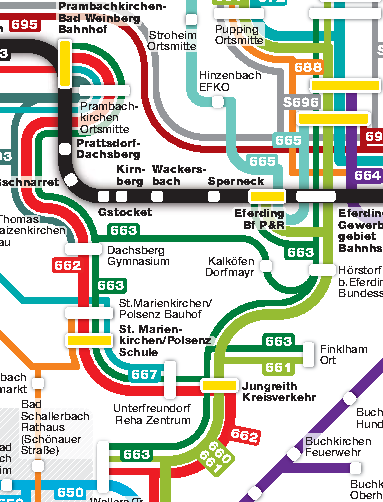
\includegraphics{liniennetzplan}}
  \caption{Ein Ausschnitt aus dem Liniennetzplan \emph{Eferding -- Grieskirchen -- Wels}, Österreich~\cite{waldherr-14}.}
  \label{fig:liniennetzplan}
\end{figure}

Um dieses Problem zu lösen, glättet man die Knicke mit Kreisbögen. Man redet dann von glatt"=orthogonalen Zeichnungen. Die Kreisbögen gehen tangential in die orthogonal verlaufenden geraden Abschnitte über. Die entstehenden Zeichnungen wirken übersichtlich, freundlich und ästhetisch, was für ansprechende Visualisierungen förderlich ist. Dadurch, dass die Kanten ansonsten trotzdem orthogonal verlaufen, bleibt die Komplexität der Layouts vergleichsweise gering. Man vergleiche hierzu etwa die in Handarbeit gefertigten Soziogramme des Künstlers Mark Lombardi (1951--2000), die u.a. aufgrund ihrer runden Kanten eine gewisse Ästhetik erreichen, jedoch mangels orthogonaler Gitterstruktur wenig Systematik erkennen lassen. 

Bestehende Algorithmen zur automatisierten Erstellung glatt"=orthogonaler Zeichnungen bauen auf bewährten Algorithmen für orthogonale Zeichnungen auf und erweitern diese so, dass genügend Platz für die abgerundeten Kanten bleibt, ohne dabei Kantenüberschneidungen einzuführen. Als Grundlage wählt man Algorithmen, welche die Anzahl der Knicke (auch pro Kante) in der entstehenden Zeichnung klein halten. Hier wird der Algorithmus von Biedl~\& Kant~\cite{biedl+kant-98} bzw.\ Liu et al.~\cite{liu+etal-98} verwendet.

Beim Zeichnen mit glatt"=orthogonalen Kanten müssen neue Herausforderungen angegangen werden. Ebenso wie Knicke in orthogonalen Zeichnungen für erhöhte Komplexität sorgen, sind in glatt"=orthogonalen Zeichnungen Wechsel zwischen geraden und gekrümmten Abschnitten und zwischen Abschnitten aus Bögen mit unterschiedlichen Radien zu vermeiden. Gleichzeitig sollte die Fläche der Zeichnung nicht zu groß werden.

Es wäre trivial möglich, alle Kanten abzurunden, indem man Kreisbögen mit dem Radius der Gittergröße einfügt. So würden neben den Kreisbögen gerade Stücke über bleiben. Daher versucht man die Kreisbögen größer zu machen und so geschickt anzuordnen, dass möglichst wenige Wechsel zwischen verschiedenen Segmenten benötigt werden. Die größeren Radien bedeuten aber auch mehr Platzbedarf, was Quelle für Kanten-Überschneidungen sein kann und die Zeichnung vergrößert. Die entstandene Zeichnung muss also angepasst werden. Dazu wurde von Alam et al.~\cite{smooth-13} bereits ein Algorithmus entwickelt, der allerdings bisher noch nicht implementiert wurde. Wir teilen die glatt"=orthogonalen Zeichnungen in Abhängigkeit der maximalen Anzahl~$k$ von Segmenten in einer Kante in die Klasse SC$_k$ ein und wollen SC$_2$-Zeichnungen erstellen.

\section{Ziel}

Diese Arbeit hat zum Ziel, Implementierungsdetails des Algorithmus von Alam et al. zum Erstellen glatt"=orthogonaler Zeichnungen auszuarbeiten. Die Implementierung ermöglicht es, für eine Reihe von Beispielgraphen glatt"=orthogonale Layouts zu erstellen, drei davon zeigt Abbildung~\ref{fig:introDemoGraphs}. Besonders interessante Zeichnungen werden gezeigt, sie sollen die Nützlichkeit von glatt"=orthogonalen Layouts unterstreichen und als Inspiration für die praktische Anwendung des Algorithmus dienen. Außerdem soll die Effektivität des Algorithmus mit empirischen Daten untersucht werden. Dabei werden eventuelle Probleme aufgezeigt, die wiederum als Grundlage zur Verbesserung des Algorithmus dienen. 

\begin{figure}[h]
  \centering
  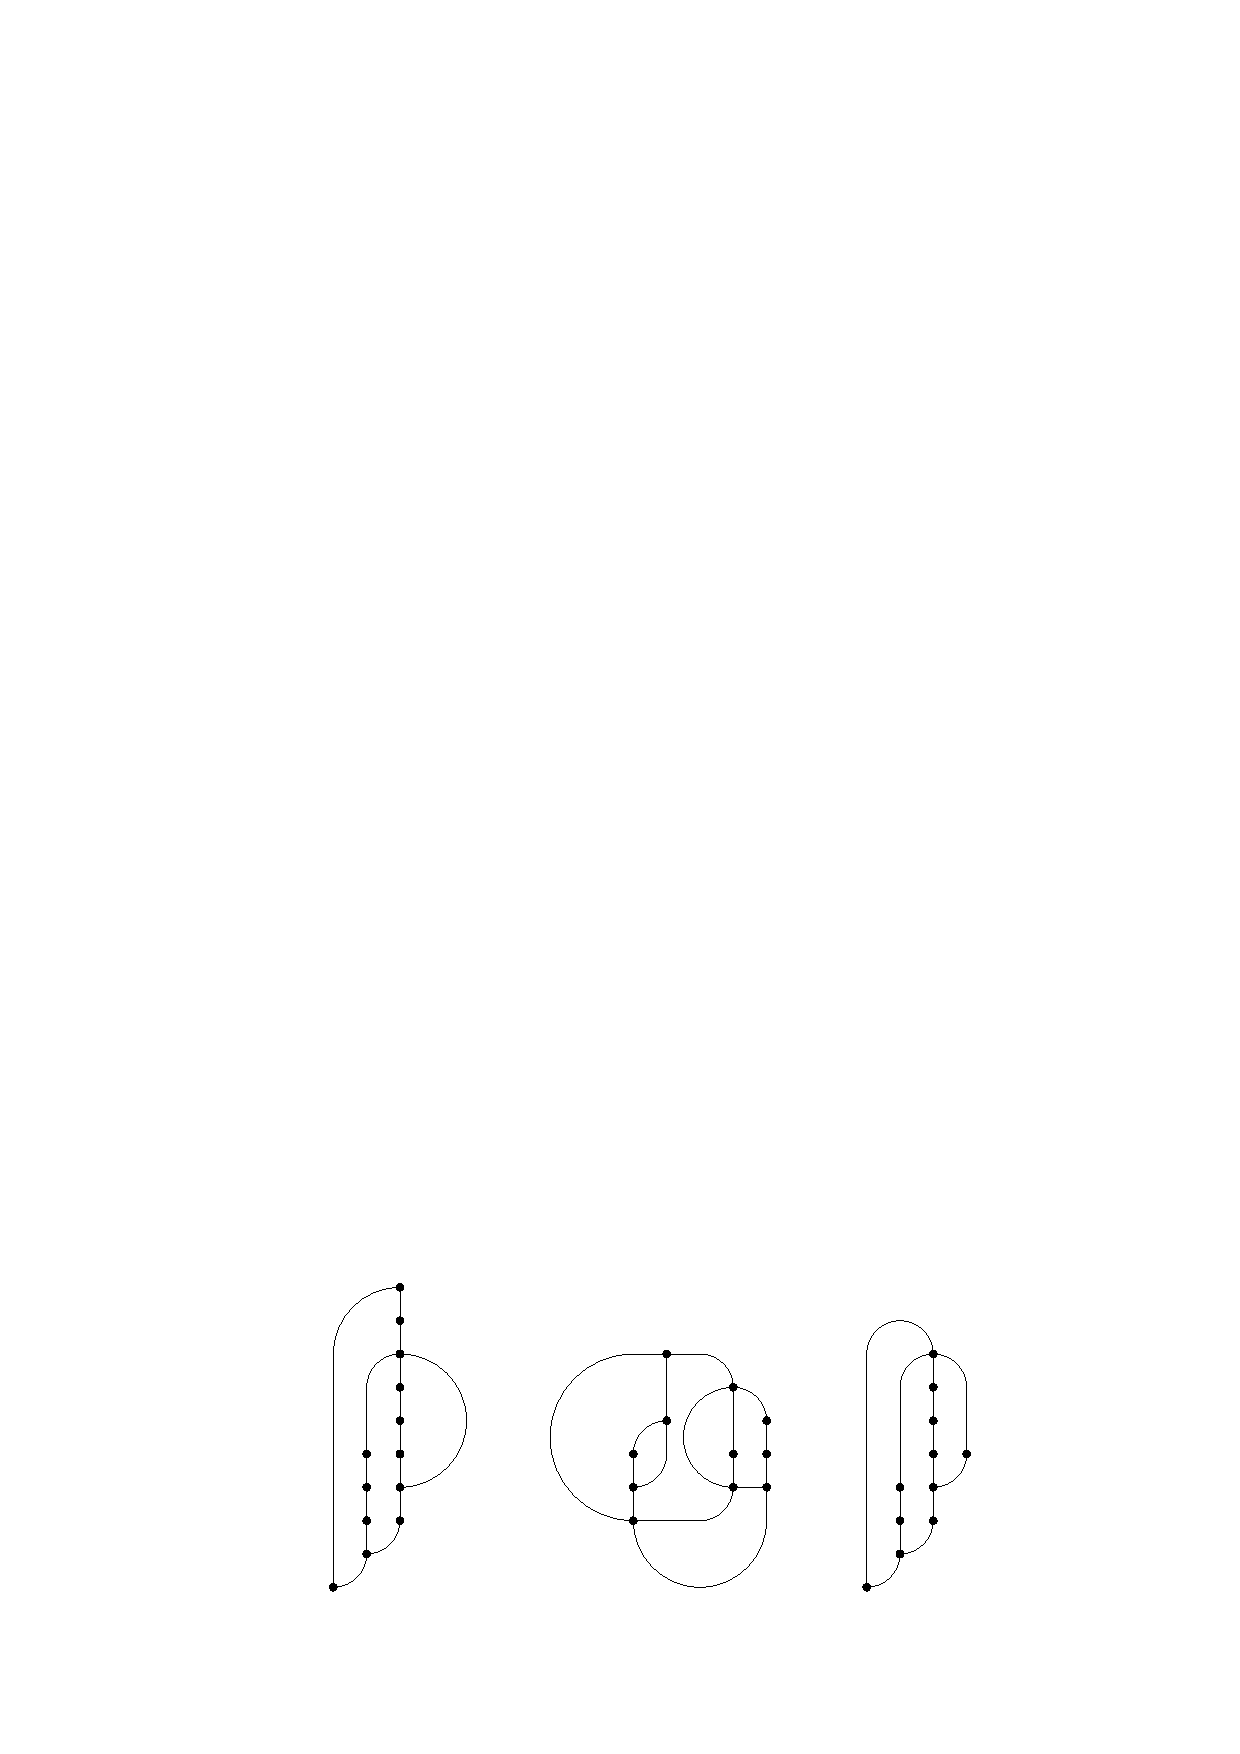
\includegraphics{intro_graphs}
  \caption{Drei glatt"=orthogonale Zeichnungen, die mit dem hier implementierten Algorithmus gezeichnet wurden}
  \label{fig:introDemoGraphs}
\end{figure}


\section{Struktur}

Zunächst werden einige Grundlagen erklärt, ohne die eine präzise Beschreibung des Algorithmus nicht möglich ist.  Das bedeutet, es werden die verwendeten Definitionen genannt und die Notationen eingeführt. Außerdem wird der Problembereich weiter eingeschränkt, während die einzelnen Konzepte aufgezählt werden. Dies bildet Kapitel~\ref{chap:basics}.

Als nächstes wird der Algorithmus verständlich und so vollständig wie nötig erklärt. Somit kann in den späteren Abschnitten auf die verschiedenen Schritte Bezug genommen werden. Damit der Leser ein umfassendes Bild des Algorithmus vermittelt bekommt, werden die Schritte zur Berechnung der Eingaben für den Algorithmus beschrieben, gefolgt vom Ausgangs-Algorithmus für orthogonale Layouts in Abschnitt~\ref{sec:oc3algo}. Die Entfernung stufenförmiger Kanten, ein später wichtiger Teilaspekt von orthogonalen Layouts, wird in Abschnitt~\ref{sec:sEdgeRemoveAlgo} erklärt. Sind alle Voraussetzungen für die Erstellung glatt"=orthogonaler Layouts geklärt, wird die Konversion in ein glatt"=orthogonales Layout beschrieben, in Abschnitt~\ref{sec:sc2conversion} und Abschnitt~\ref{sec:sc2makePlanarAlgo}. Diese Beschreibungen rund um die Teile des Algorithmus füllen Kapitel~\ref{chap:algo}.

Darauf folgen die Implementierungsdetails des Algorithmus und einige vertiefende Beschreibungen, welche Besonderheiten sowie Herausforderungen zu beachten waren, die nötigen Datenstrukturen werden konkretisiert und gelöste Teilprobleme im Kapitel~\ref{chap:impl} erörtert. Insbesondere dem Finden von Schnitten gebührt ein eigener Text, der Abschnitt~\ref{sec:cutfinding}.

Im Anschluss wird die Implementierung mit verschiedenen Testdatensätzen kontrolliert. Anhand der Analyse der Ausgabe-Zeichnungen für die Testgraphen werden Schwachstellen des Verfahren identifiziert. Zuletzt werden noch einige Verbesserungsmöglichkeiten diskutiert und ihre Effektivität gemessen. Sie optimieren das Ergebnis im Hinblick auf Komplexität und Platzbedarf. Damit schließt das Kapitel~\ref{chap:results}.

Abgerundet wird der Text durch das zusammenfassende Kapitel~\ref{chap:outro}.





\chapter{Grundlegendes}
\label{chap:basics}

In diesem Abschnitt sollen einige Grundlagen definiert werden. Zu jedem Begriff gibt es eine knappe Definition und einige Anmerkungen zur Relevanz für den Algorithmus. So wird die Problemstellung im Verlauf dieses Abschnittes immer klarer und im nächsten Abschnitt kann der Algorithmus mit den definierten Grundlagen präzise beschrieben werden.

\section{Graphen}

Zuerst sollte natürlich definiert werden, was überhaupt visualisiert werden soll:

\begin{definition}
  Ein \emph{(ungerichteter) Graph} $G$ ist ein Tupel $(V, E)$ von Mengen, wobei $E \subset \mathcal{P}(V)$.
  Die $v \in V$ heißen \emph{Knoten}, die $e \in E$ \emph{Kanten}.
\end{definition}

Graphen bilden die Eingabe für die Zeichenalgorithmen. Die hier behandelten Graphen beschreiben Verbindungen zwischen Elementen als Kanten zwischen Knoten. 

\begin{example}
  \label{ex:graph}

Der Graph $G_\text{E}$, an dem fortan verschiedene Konzepte illustriert werden, ist definiert durch:

\[G_\text{E} = (V_\text{E}, E_\text{E})\]
\[V_\text{E} = \{0, 1, 2, 3, 4\}\]
\[E_\text{E} = \{\{0, 1\}, \{0, 2\}, \{0, 4\}, \{1, 2\}, \{1, 4\}, \{2, 3\}, \{2, 4\}, \{3, 4\}\}\]

Hier wären 1, 2 und 3 Beispiele für Knoten und $\{0, 1\}$ wäre eine Kante.
\end{example}

Der Fokus liegt auf ungerichteten einfachen Graphen, das bedeutet, es gibt zwischen zwei Knoten jeweils nur höchstens eine Kante und eine \emph{Schleife}, also eine Kante mit $|e| = 1$ kommt nicht vor.

Einfache Graphen können im Computer als \emph{Adjazenzmatrix} $(a_{i,j})$ dargestellt werden, mit $a_{i,j} = 1$ falls $\{v_i, v_j\} \in E$ und $0$ sonst. Hier wird jedoch $O(|V|^2)$ Speicherplatz verwendet. Für Graphen mit vergleichsweise wenigen Kanten eignet sich die Darstellung als \emph{Adjazenzliste} $A$ mit $A(v) = \{e \in E \mid v \in e\}$. Hierfür wird $O(|V| + |E|)$ Speicher benötigt. Im Graphen $G_\text{E}$ wäre z.B.\ $A(3) = \{2,4\}$. % TODO: Speicher genau Checken!!!

\section{Orthogonale Visualisierungen von Graphen}
\label{sec:orthogonalDrawings}

\begin{figure}[h]
        \centering
        \begin{subfigure}[b]{0.4\textwidth}
                \centering
                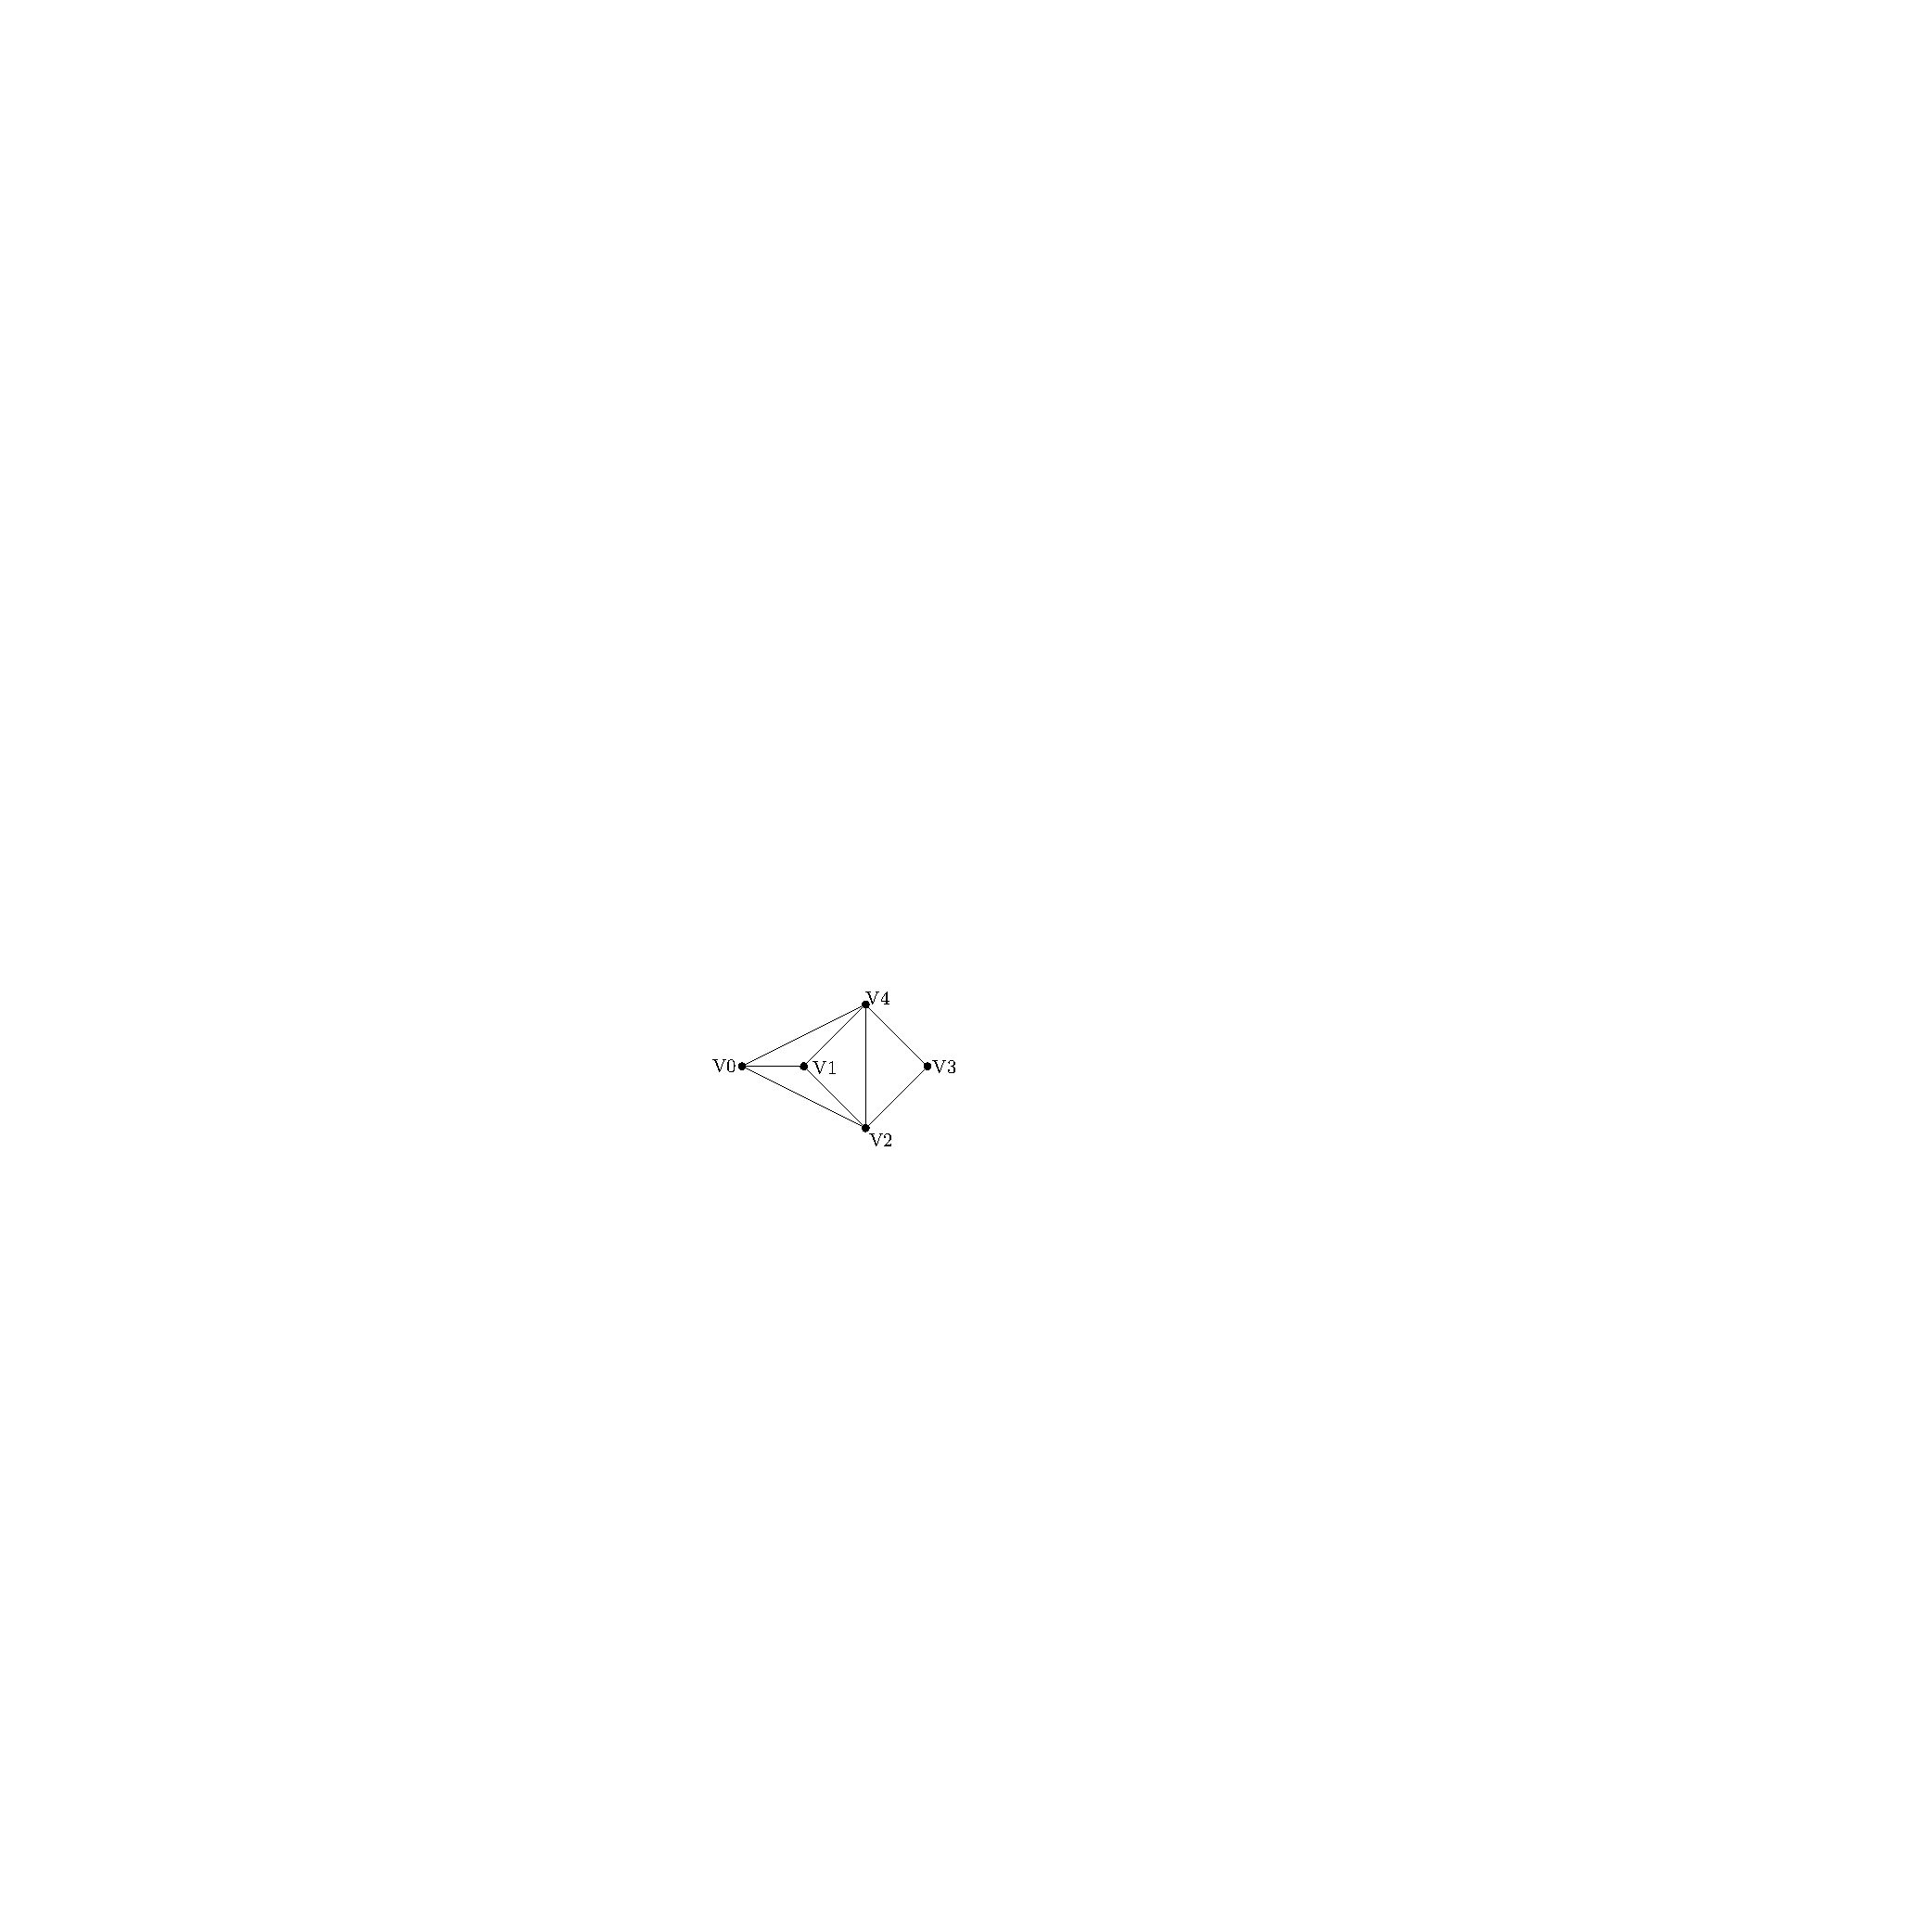
\includegraphics[width=0.6\textwidth]{exampleA/straightline}
                \caption{Ohne Überschneidungen.}
                \label{fig:exampleAstraightline}
        \end{subfigure}
        \quad
        \begin{subfigure}[b]{0.4\textwidth}
                \centering
                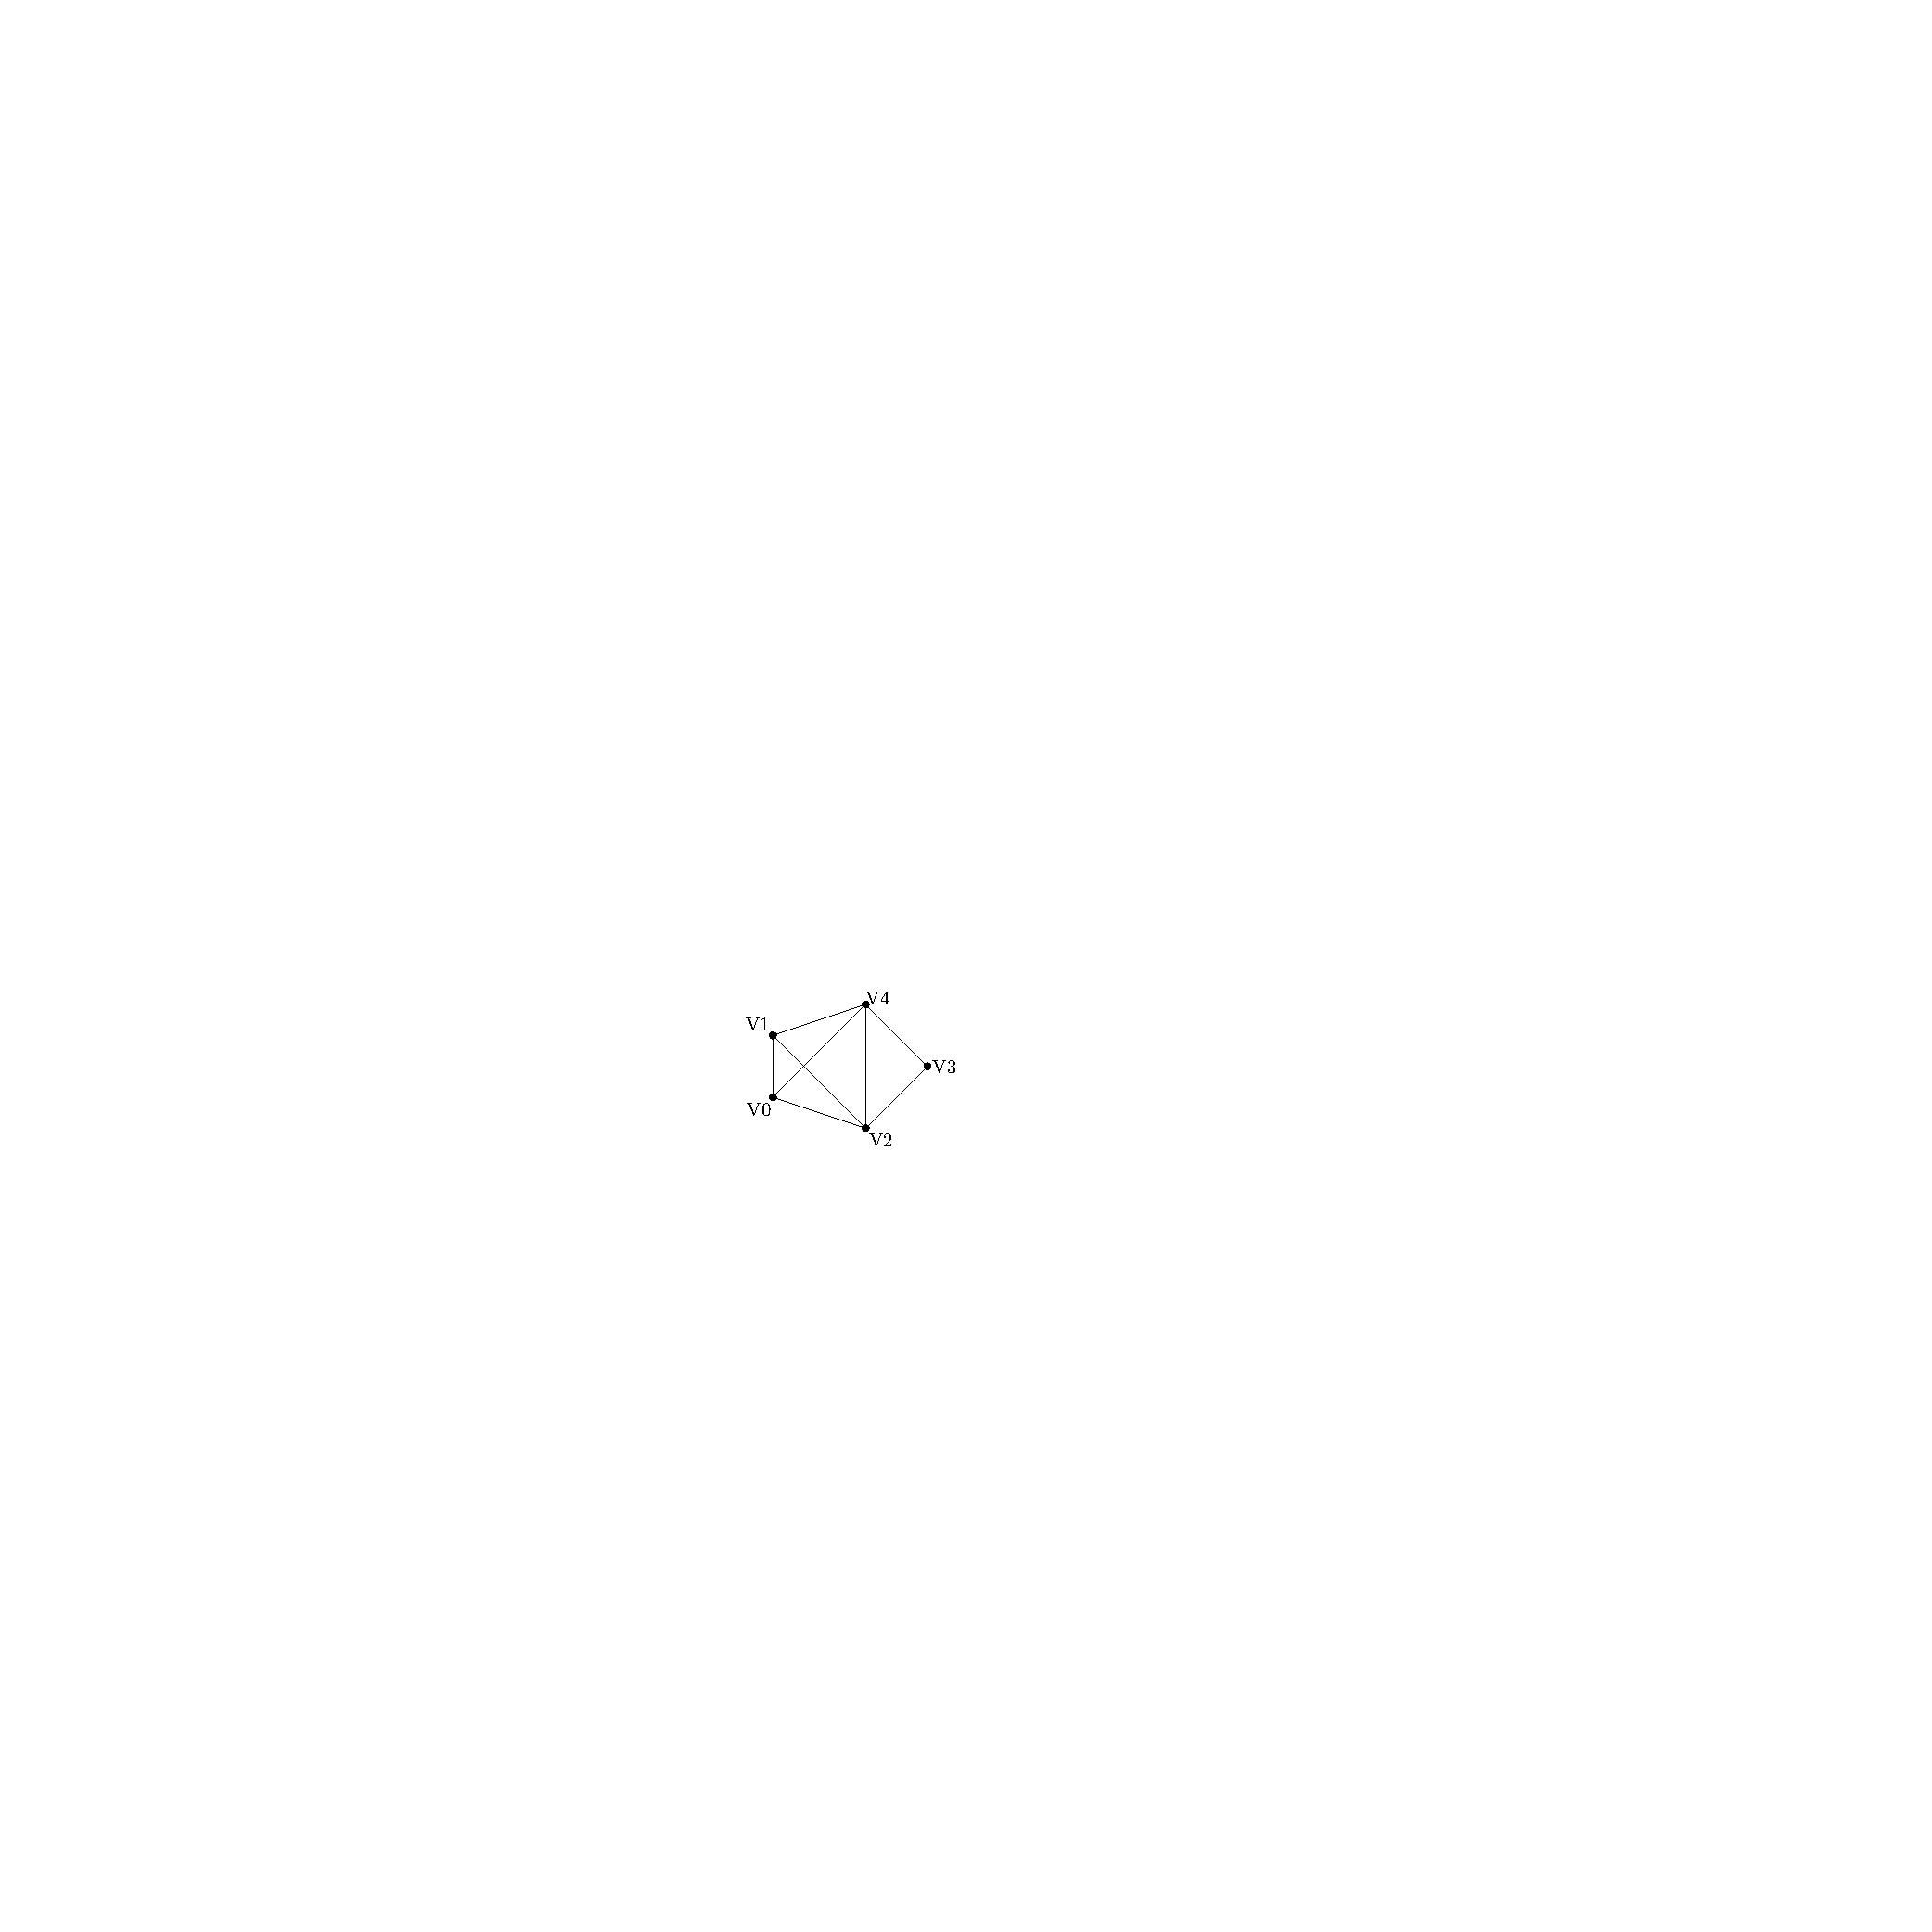
\includegraphics[width=0.52\textwidth]{exampleA/straightlineNonplanar}
                \caption{Mit Überschneidungen.}
                \label{fig:exampleAstraightlineNonplanar}
        \end{subfigure}
        \caption{Zwei Zeichnungen des Graphen $G_\text{E}$ aus Beispiel~\ref{ex:graph}. Zur besseren Übersicht sind die Knoten mit \emph{V} und ihrer Nummer beschriftet.}
\end{figure}


Die Darstellung von einfachen Graphen für Menschen, die \emph{Zeichnung} oder \emph{Visualisierung}, besteht üblicherweise aus Punkten, also kleinen Kreisen, für jeden Knoten und Verbindungslinien für die Kanten. Die Überführung von einer Adjazenzliste in einer solche Darstellung nennt man das \emph{Zeichnen} von Graphen. Hierfür gibt es keine kanonische Vorgehensweise. Der umgekehrte Weg von der Zeichnung zur Adjazenzliste jedoch ist (bei geeigneten Zeichnungen) eindeutig und trivial zu lösen.

Eine Zeichnung des Beispielgraphen $G_\text{E}$ findet sich in Abbildung~\ref{fig:exampleAstraightline}.

Für \emph{Multigraphen} mit mehreren Kanten zwischen zwei Knoten kommen Variationen der Zeichnungen für einfache Graphen in Frage, die solche Kanten als Bündel oder dicker darstellen. Sie sollen daher hier nicht behandelt werden und einfache Graphen werden im Folgenden kurz als Graphen bezeichnet.

\begin{figure}[h]
  \centering
  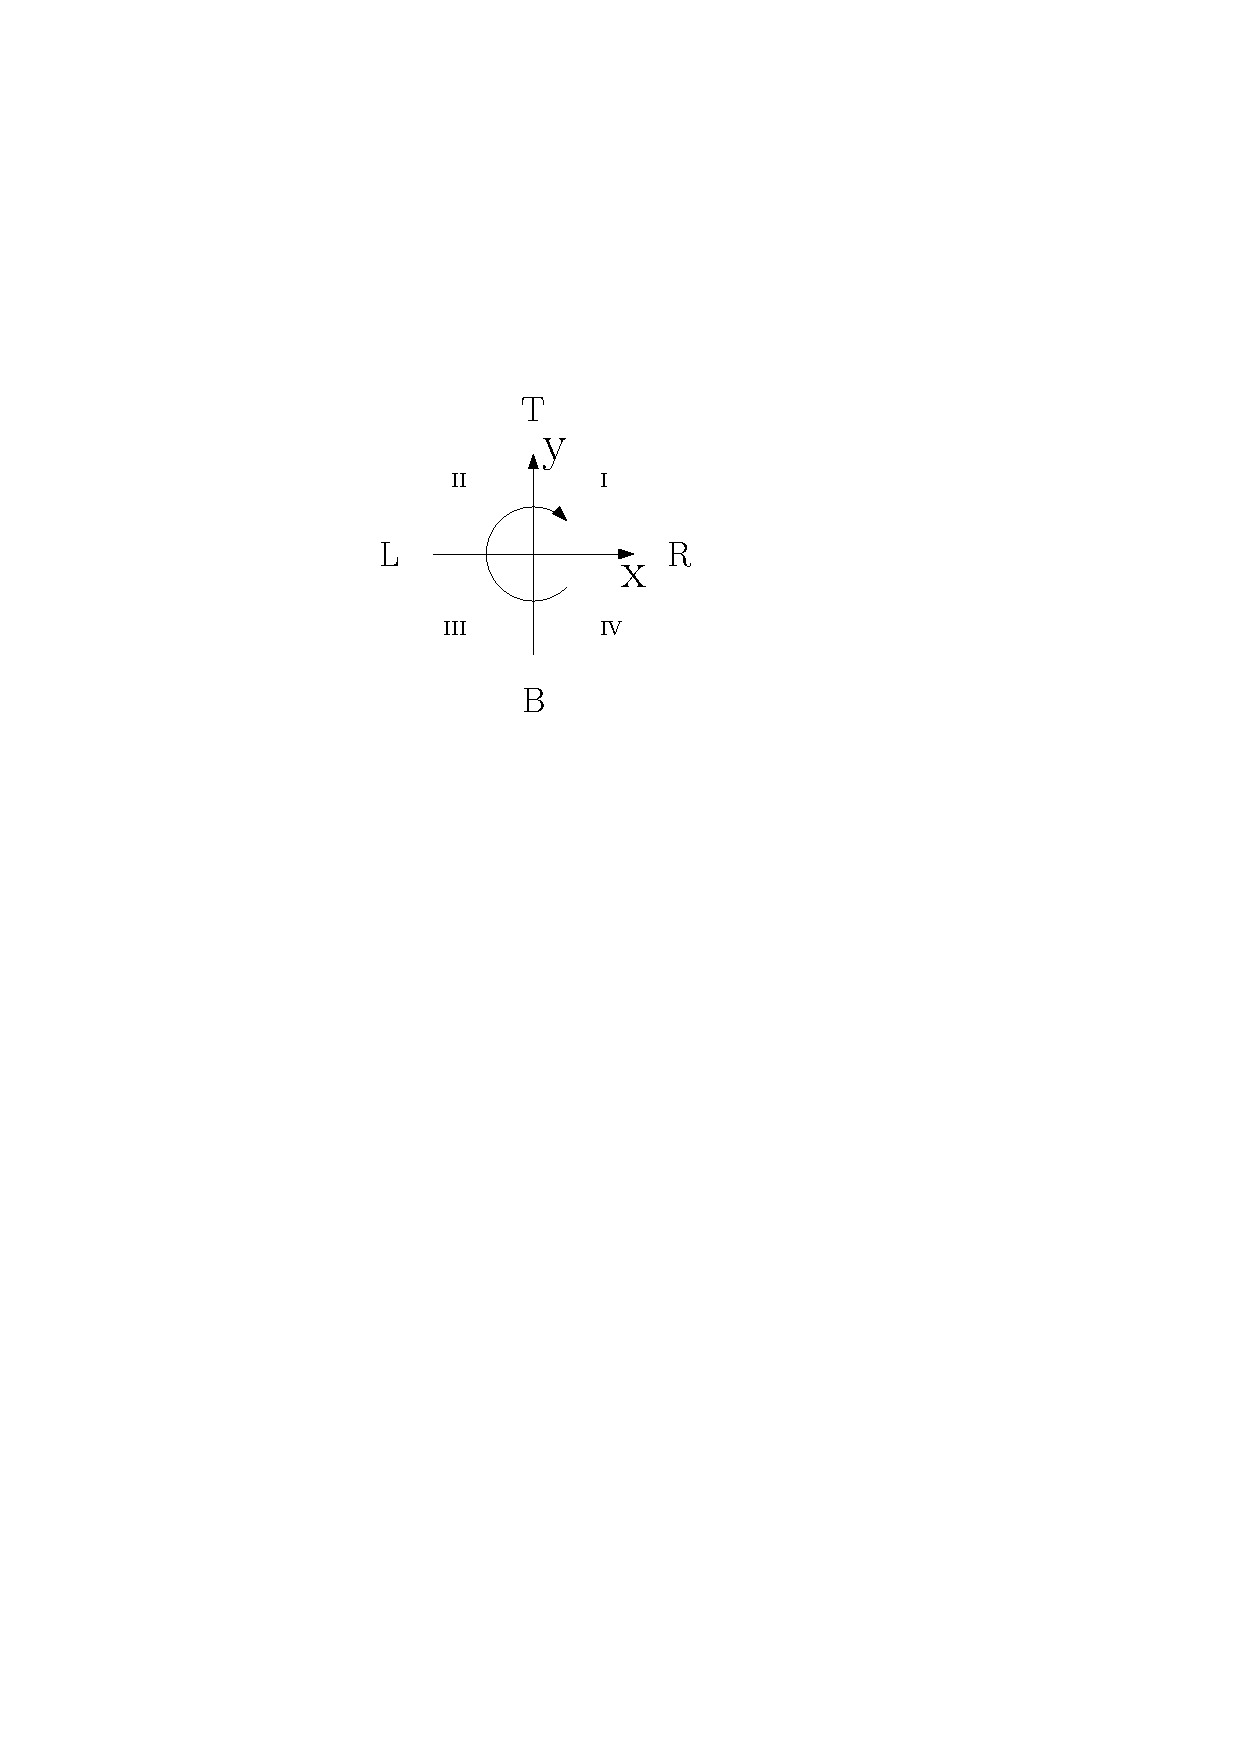
\includegraphics[scale=.6]{koordinatengitter}
  \caption{Gezeichnet wird in eine Koordinatenebene. Hier wird die Anordnung der beiden Koordinaten-Achsen gezeigt, die Richtungen der Ports $\{\text{L, R, T, B}\}$, der Drehsinn der Anordnung im Uhrzeigersinn der Adjazenzlisten und die Quadranten $\{\text{I, II, III, IV}\}$.}
  \label{fig:coords}
\end{figure}

\begin{definition}
  \label{def:layouts}
  Ein (zweidimensionales) \emph{Layout} $L$ über einer Menge $V$ ist eine Abbildung $L_V : V \to \N \times \N $. Ein \emph{Port} p ist eine Element der Menge \{\text{L, R, T, B}\}. Eine \emph{Portzuweisung} $P$ ist eine Abbildung $P: \{(v, e) \in V \times E \mid v \in e\} \to \{\text{L, R, T, B}\}$. Ein \emph{orthogonales Layout} ist ein 3"~Tupel $(L_V,L_E,P)$ von Layouts $L_V$ und $L_E$ und einer Portzuweisung $P$.
\end{definition}

Die Hauptaufgabe eines Zeichenalgorithmus ist die Positionierung der Knoten auf einer Zeichenebene. Die berechnete Positionszuweisung heißt Layout. In einer \emph{geradlinigen Zeichnung} werden die Kanten als gerade Linien zwischen den Knoten gezeichnet. Hier bestimmt also die Position der Knoten vollständig das Aussehen der Kanten.

Bei orthogonalen Zeichnungen bestehen die Kanten aus horizontalen und vertikalen Segmenten entlang des Koordinatengitters der Zeichenebene. Zwei verschiedene orthogonale Zeichnungen des Beispielgraphen $G_\text{E}$ finden sich in Abbildung~\ref{fig:exampleAorthogonal}.

\begin{figure}[h]
  \centering
\begin{subfigure}[b]{0.4\textwidth}
  \centering
  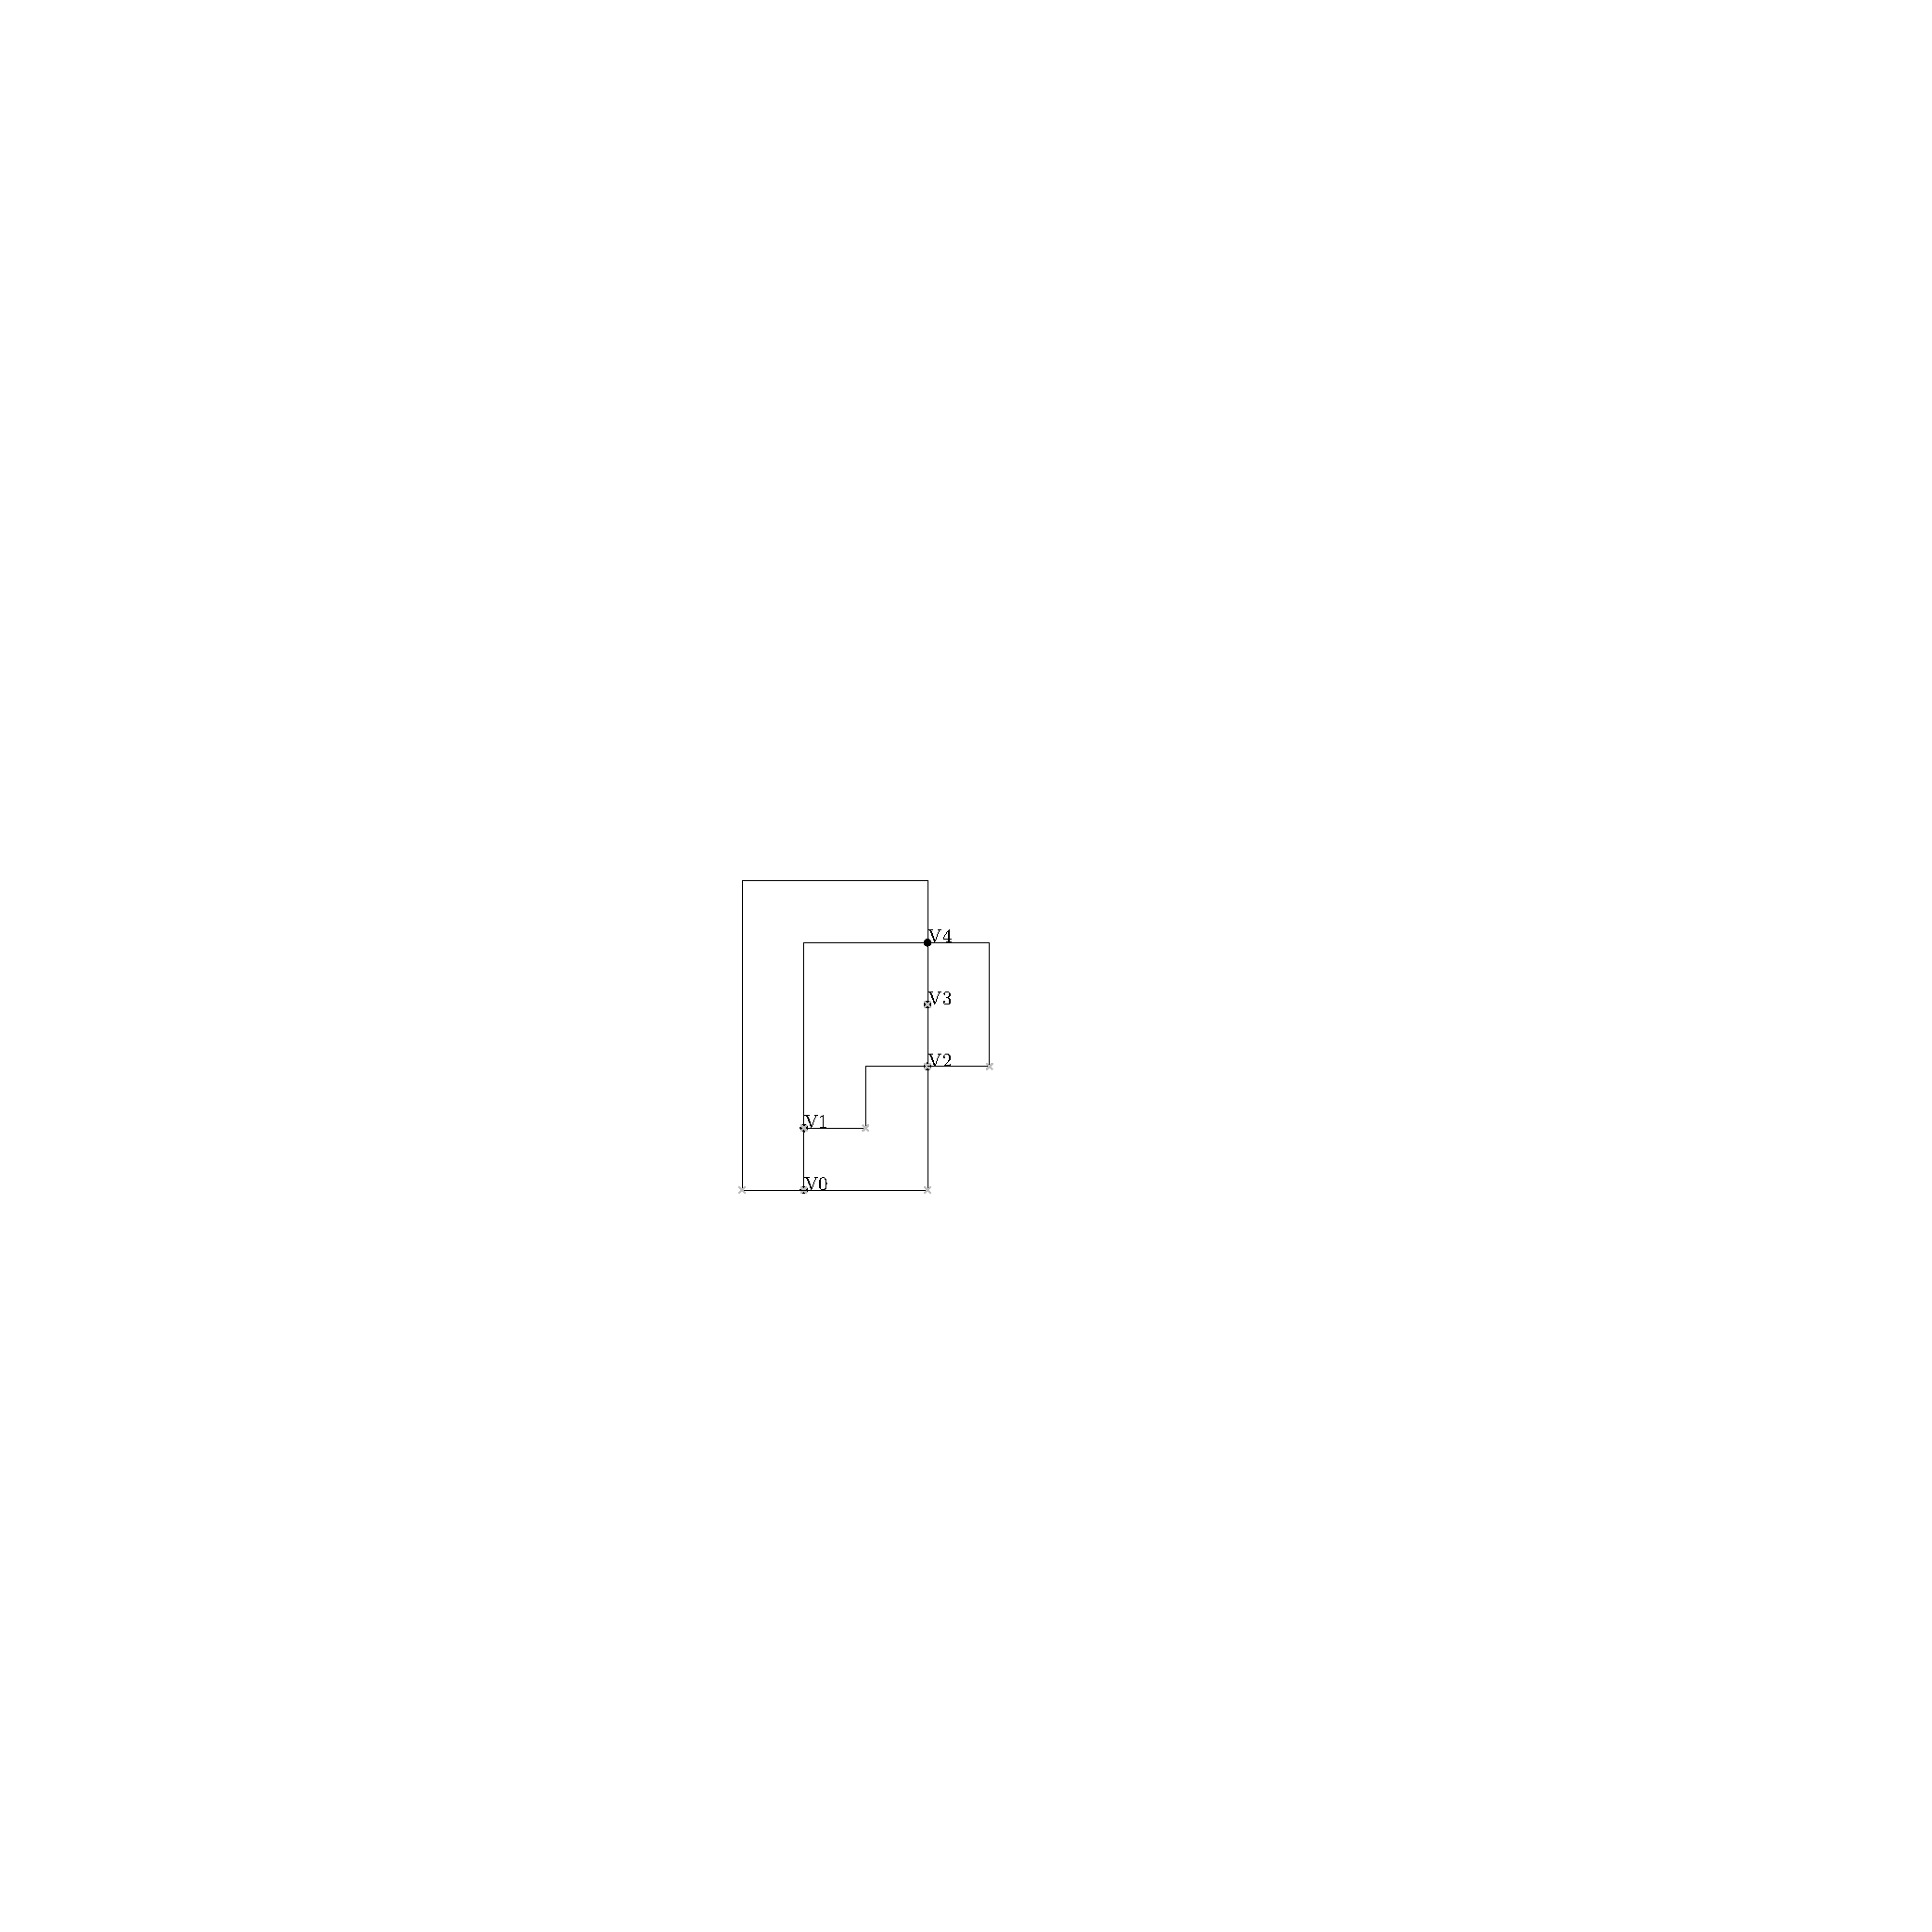
\includegraphics{exampleA/orthogonalNocompress}
  \caption{Mit stufenförmiger Kante $\{0,4\}$.}
  \label{fig:exampleAorthogonalNocompress}
\end{subfigure}
  \quad
\begin{subfigure}[b]{0.4\textwidth}
  \centering
  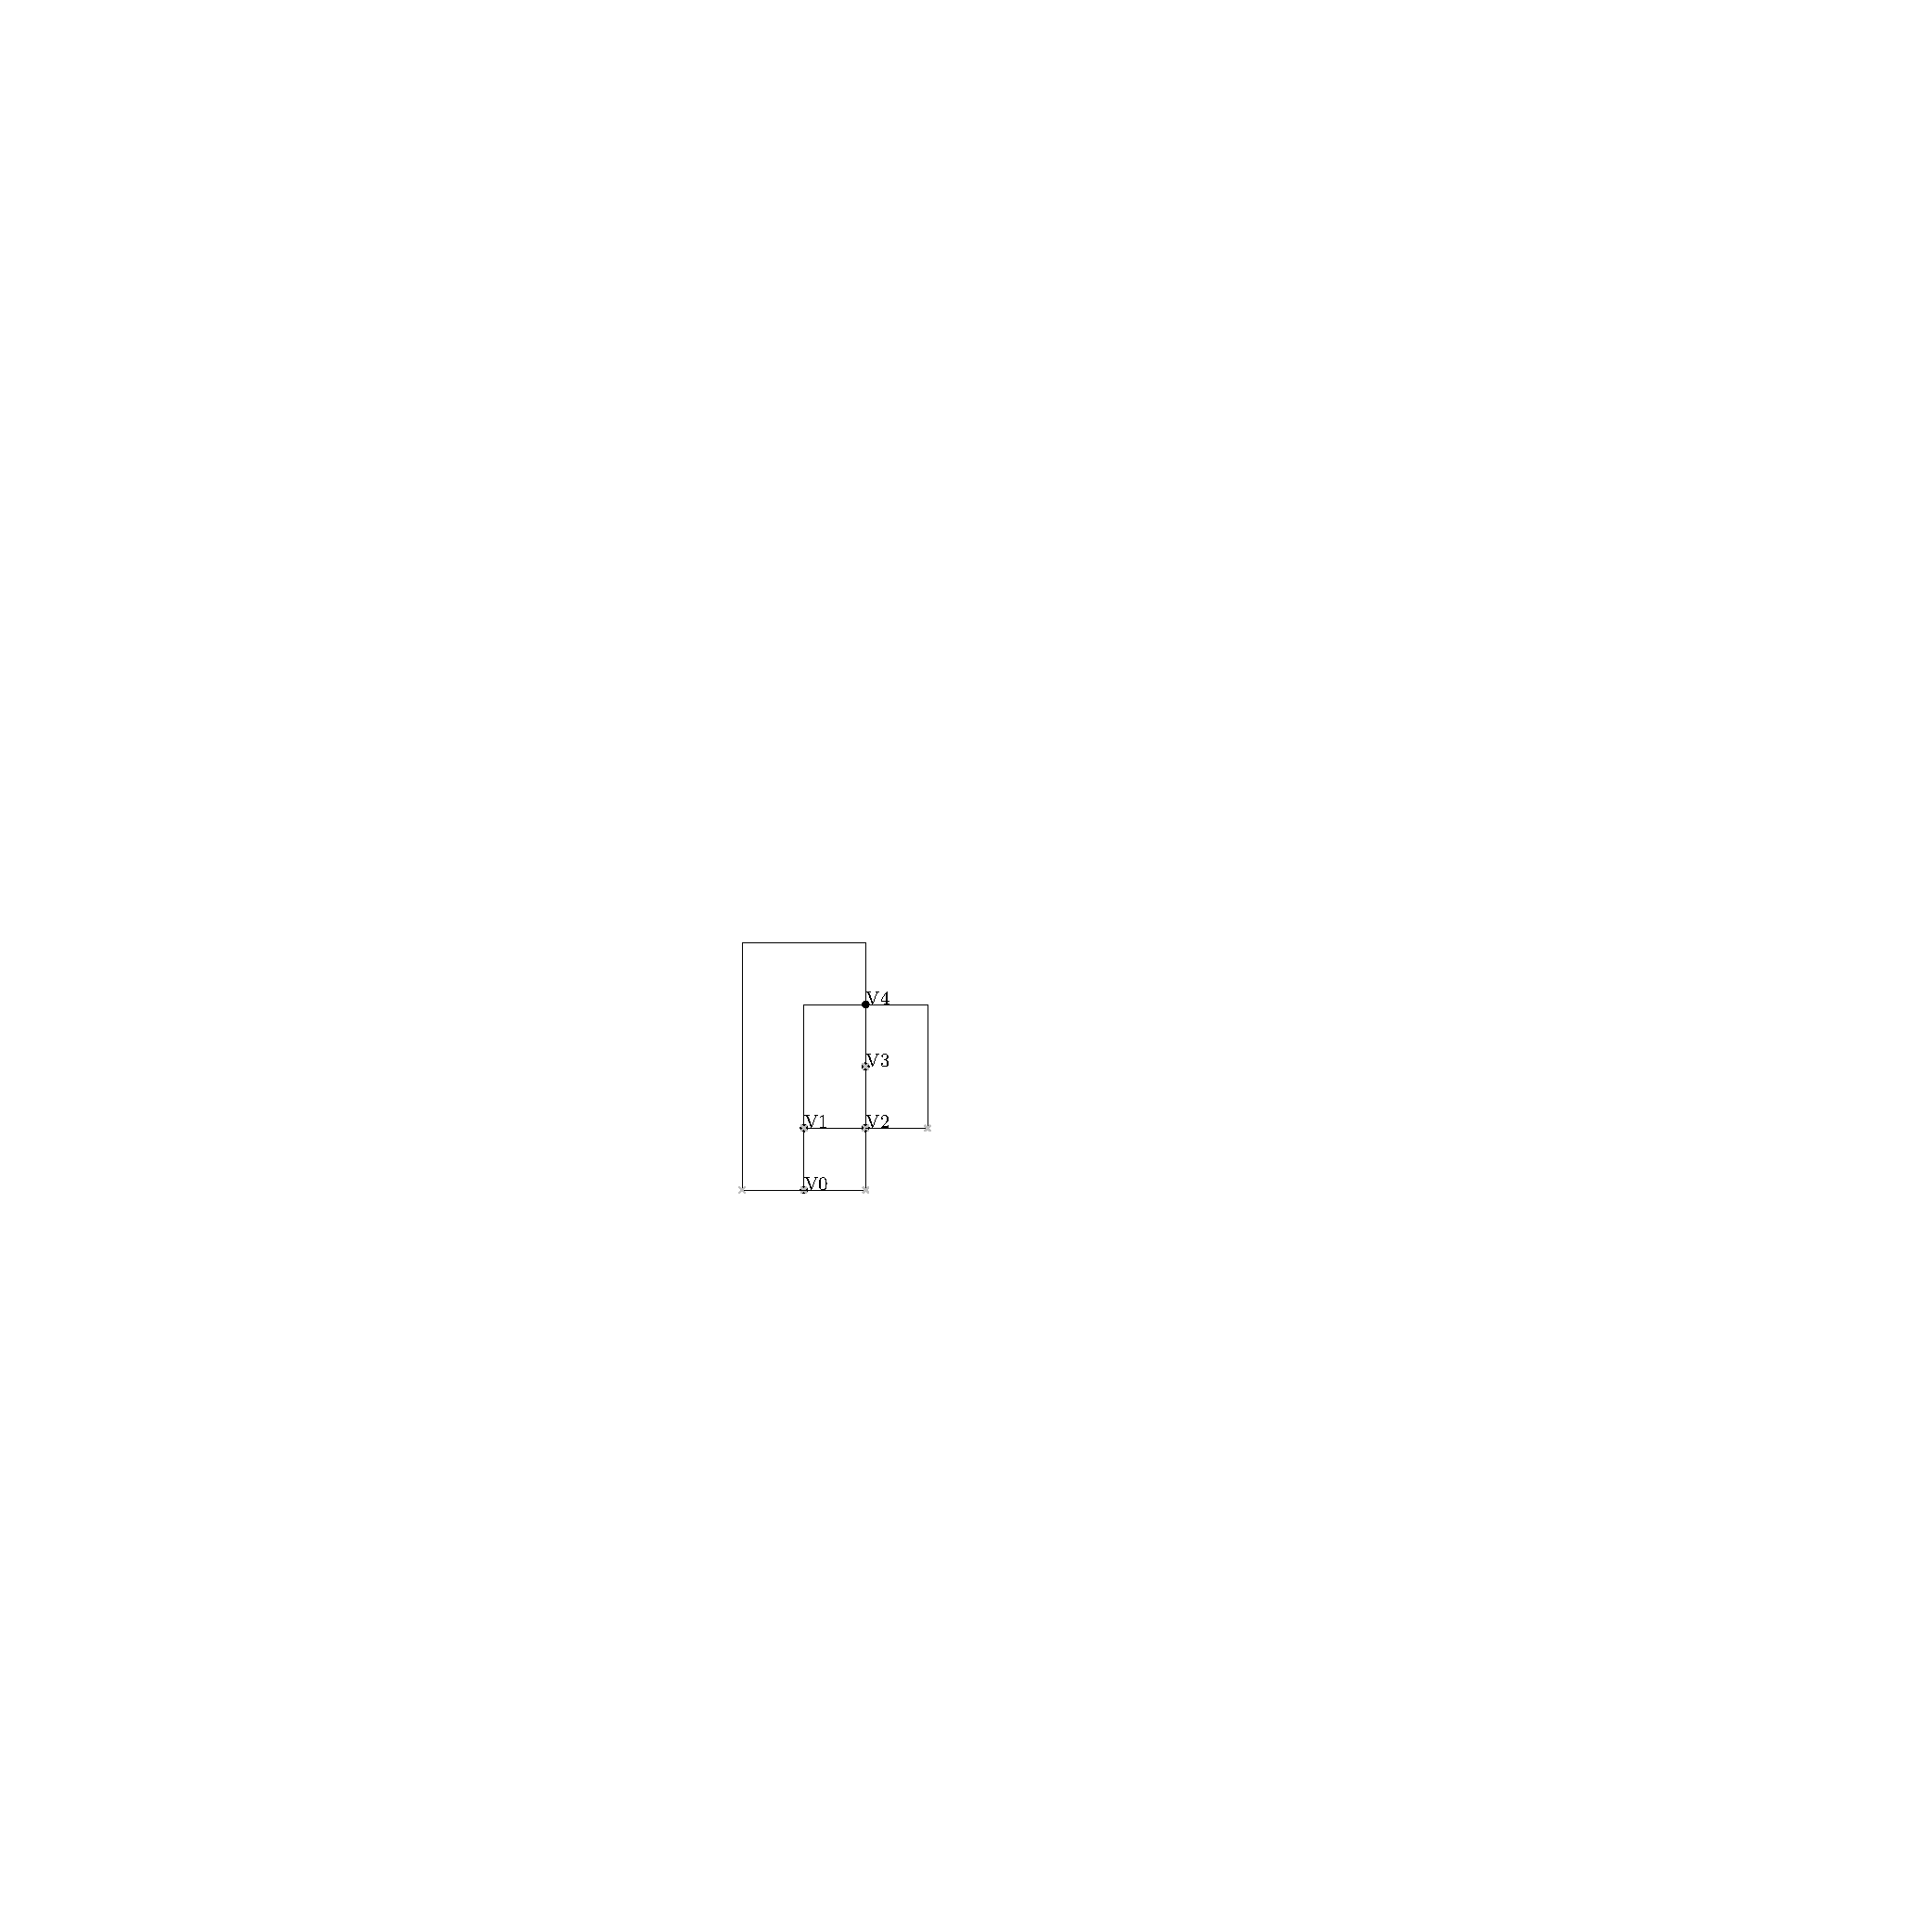
\includegraphics{exampleA/orthogonalCompress}
  \caption{Ohne stufenförmige Kanten.}
  \label{fig:exampleAorthogonalCompress}
\end{subfigure}

  \caption{Der Graph $G_\text{E}$ aus Beispiel~\ref{ex:graph} in orthogonalen Zeichnungen. Graue Kreuze markieren die Orte der Kanten.}
  \label{fig:exampleAorthogonal}
\end{figure}

Bei orthogonalen Zeichnungen gibt es eine Vielzahl von Möglichkeiten für das Aussehen der Kanten: An den Gitterpunkten kann entweder zuerst horizontal oder zuerst vertikal weiter gezeichnet werden. Wird immer abwechselnd horizontal und vertikal gezeichnet, entstehen viele Knicke in den Kanten. Man gibt die \emph{Komplexität} einer orthogonalen Zeichnung in Abhängigkeit der größten Anzahl von Segmenten $k$ in einer Kante dieser Zeichnung an, und nennt sie dann eine \emph{$\text{OC}_k$-Zeichnung}. Die Abbildung~\ref{fig:exampleAorthogonal} enthält somit zwei OC$_3$-Zeichnungen, da die Kante $\{0,4\}$ jeweils aus drei Segmenten besteht.

Eine Möglichkeit, das Aussehen der Kanten zu normieren und gleichzeitig die Anzahl der Knicke zu minimieren, wäre es, immer den vollständigen horizontalen Weg am unteren Knoten und dann den vertikalen Weg nach oben zu zeichnen, sodass jede Kante L"~förmig ist. Hierbei kommt es jedoch zu Überschneidungen, wenn beispielsweise zwei Kanten einen Knoten in dieselbe Richtung verlassen. Überschneidungen sorgen für Zweideutigkeiten in der Zeichnung und sollen vermieden werden. Deshalb weist man den Kanten an jedem Knoten einen Port aus der Menge $\{\text{L, R, T, B}\}$, also Links, Rechts, Top (oben) oder Bottom (unten) zu. Die Richtungen der Ports sind auch in Abbildung~\ref{fig:coords} zu erkennen.\\


Das Zeichnen einer Kante $e$ eines Graphen $G = (V,E)$ in einem orthogonalen Layout $(L_V,L_E,P)$ kann nun so erfolgen: Von den von $L_V$ gegebenen Positionen der beiden Endknoten $v \in e$ wird eine Gittereinheit in der Richtung des Ports gezeichnet. Von diesen Positionen aus wird je eine horizontale Linie bis zur x"~Koordinate des von $L_E$ gegebenen Kantenorts gezeichnet. Die beiden Endpositionen werden mit einer vertikalen Linie verbunden.\\ %% TODO: Proof?


Es können jedoch immer noch Überschneidungen von Kanten an einem Knoten $v \in V$ auftreten, wenn die Ports kollidieren, wenn es also zwei Kanten $e_1, e_2 \in E$ mit $P(v, e_1) = P(v, e_2)$ gibt. Da es nur vier Ports gibt, können somit nur maximal vier Kanten mit einem Knoten verbunden sein.

\begin{definition}
  Die Anzahl $deg(v) = |\{e \in E \mid v \in e\}|$ ist der \emph{Grad} eines Knotens. Der Wert $deg(G) = \max_{v \in V}{deg(v)}$ eines Graphen $G = (V, E)$ ist der Grad des Graphen.
\end{definition}

Im Beispielgraphen $G_\text{E}$ wäre $deg(G) = 4$ und $deg(0) = 3$, $deg(1) = 3$, $deg(2) = 4$, $deg(3) = 2$, sowie $deg(4) = 4$.

Ohne Kanten-Überschneidungen an den Knoten können also nur Graphen mit Maximalgrad~4 gezeichnet werden. 

Es kann noch immer Überschneidungen bzw.\ Kreuzungen der Kanten an anderer Stelle geben. Es gibt sogar Graphen, die sich auf keine Art und Weise ohne Überschneidungen von Kanten zeichnen lassen.


\section{Planare Graphen}

Da das Ziel des Algorithmus ist, Graphen ohne Überschneidungen zu zeichnen, stellt sich die Frage, ob es grundsätzlich möglich ist, alle Graphen überschneidungsfrei zu zeichnen oder welche Graphen sich nicht überschneidungsfrei zeichnen lassen.

\begin{figure}[h]
  \centering
  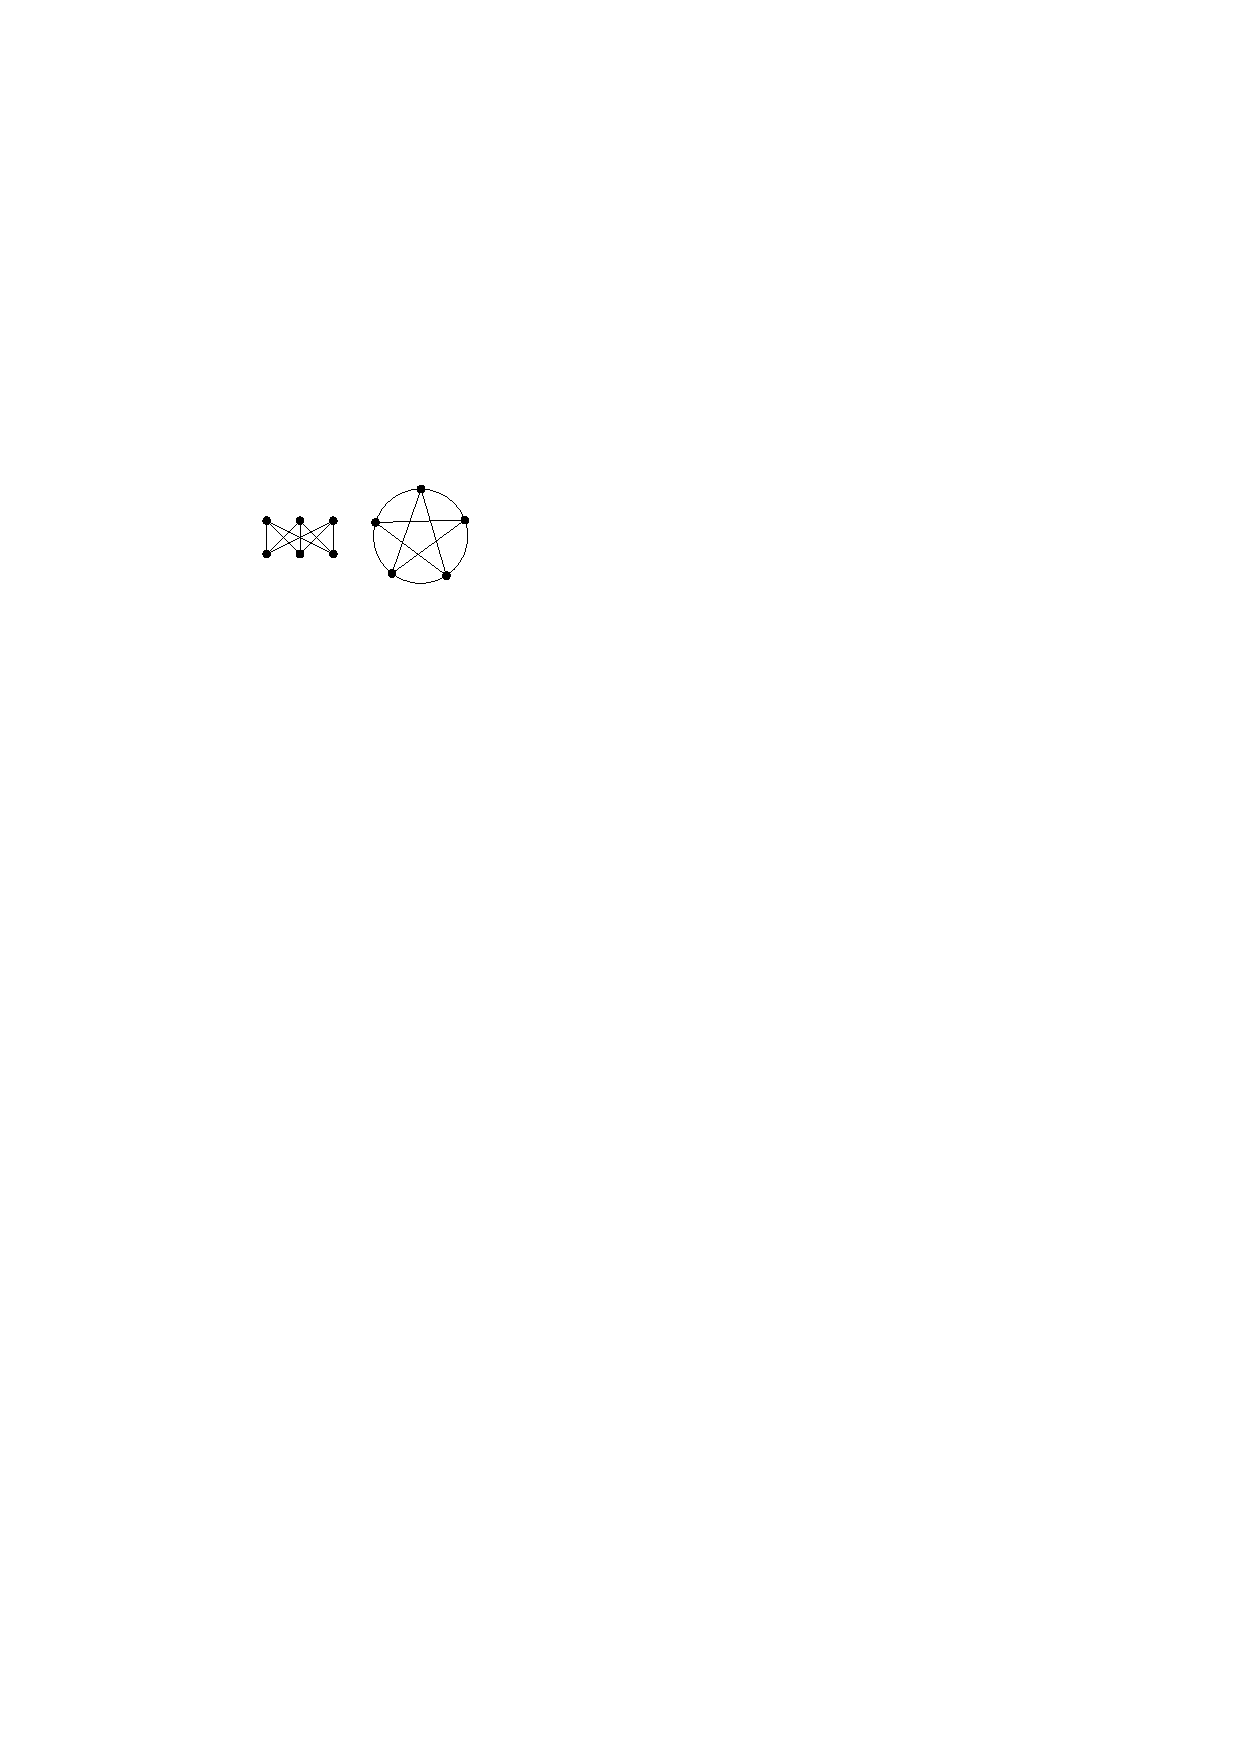
\includegraphics{nonplanar}
  \caption{Zwei Zeichnungen von Graphen, die sich nicht überschneidungsfrei zeichnen lassen, die Kuratowski-Graphen.}
  \label{fig:nonplanar}
\end{figure}

\begin{definition}
  Ein Graph $G$ heißt \emph{planar}, wenn er in der Ebene ohne Überschneidungen gezeichnet werden kann.
\end{definition}

Hierbei dürfen sich die Kanten an den Knoten berühren. Keine zwei Knoten dürfen an derselben Stelle gezeichnet werden. Für eine Zeichnung bedeutet das, dass ihr Layout $L_V$ injektiv sein muss. Das der Beispielgraph $G_\text{E}$ planar ist, haben wir bereits bewiesen, indem wir ihn ohne Überschneidungen gezeichnet haben. 

Die Graphen aus Abbildung~\ref{fig:nonplanar} jedoch lassen sich nicht ohne Überschneidung zeichnen, sie sind nicht planar. Solche nicht-planaren Graphen werden mit dem Algorithmus nicht gezeichnet. 

Für planare Graphen ist es nicht offensichtlich, wie genau sie gezeichnet werden müssen, damit sich keine Überschneidungen ergeben. Der eigentlich planare Beispielgraph $G_\text{E}$ wurde in Abbildung~\ref{fig:exampleAstraightlineNonplanar} mit Überschneidungen gezeichnet. Nach dem Satz von Fáry hat jeder planare Graphen eine Zeichnung, in der alle Kanten als gerade Linien gezeichnet sind.

In dieser Zeichnung unterteilen die Kanten die Zeichenebene in abgegrenzte Bereiche, die \emph{Facetten}. Jede Kante grenzt an zwei Facetten, auf jeder Seite eine. Die beiden Knoten der Kante grenzen ebenfalls an die beiden Facetten. Der Bereich außerhalb, der den Graphen umgibt, heißt \emph{Außenfacette}.

Die Reihenfolge der Kanten um einen Knoten im Uhrzeigersinn in dieser Zeichnung, also eine Anordnung der Adjazenzlisten, ist auf dem Weg zur überschneidungsfreien Zeichnungen ausschlaggebend.


\begin{definition}
  Eine \emph{planare Einbettung} eines Graphen $G = (V, E)$ gibt für alle $v \in V$ eine Reihenfolge der Kanten der Adjazenzliste $A(v) = \{e_1, \dots, e_n\}$ vor.
\end{definition}

In der planaren Zeichnung des Graphen $G_\text{E}$ in Abbildung~ \ref{fig:exampleAstraightline} wären z.B.\ folgende Adjazentlisten-Reihenfolgen: $A(0) = \{4,1,2\}, A(1) = \{0,4,2\}, A(2) = \{0,1,4,3\}, A(3) = \{2,4\}, A(4) = \{3,2,1,0\}, $. Zyklische Verschiebungen dieser Listen sind äquivalent.

Planare Graphen haben die Eigenschaft, dass die Anzahl der Kanten die dreifache Anzahl der Knoten nicht überschreiten kann, genauer: $|E| \leq 3 |V| - 6$. Hat ein Graph mehr als $3 |V| - 6$ Kanten, können wir also ausschließen, dass er planar ist. Wenn Algorithmen auf planaren Graphen laufen, können durch $|E| = O(|V|)$ einige Operationen, die auf allgemeinen Graphen in $O(|V| + |E|)$ Zeit laufen, in linearer Zeit $O(|V|)$ laufen. Mit Hilfe dieser Eigenschaft können wir später die Laufzeit von Teilen unseres Algorithmus mit $O(|V|)$ angeben.

Wie in Abschnitt~\ref{sec:orthogonalDrawings} gezeigt, können in orthogonalen Zeichnungen nur solche Graphen überschneidungsfrei gezeichnet werden, deren Grad maximal~4 ist. Zusätzlich können nur planare Graphen überschneidungsfrei gezeichnet werden. Man nennt Graphen, die diese beiden Bedingungen erfüllen, auch \emph{4"~planar}.

\section{Zusammenhangs-Eigenschaften von Graphen}

\begin{definition}
  Ein \emph{Teilgraph} $G'$ eines Graphen $G=(V, E)$ ist ein Graph $G' = (V' \subset V, E' \subset E))$.
  Ein \emph{induzierter Teilgraph} $G_U$ eines Graphen $G=(V, E)$ über einer Menge $U \subset V$ ist der Kanten-Maximale Graph mit $G_U = (U , E' \subset E))$.
\end{definition}

Häufig werden nur Teile eines größeren Graphen betrachtet. % TODO: mehr?

\begin{definition}
  Ein \emph{Weg} ist ein Graph $G = (V, E)$ mit $V = \{v_1, v_2, \dots, v_n\}$ und $E = \{\{v_1, v_2\}, \{v_2, v_3\}, \dots, \{v_{n-1}, v_{n}\}\}$.
  Es gibt in einem Graphen $G = (V, E)$ einen Weg zwischen zwei Knoten $v_\text{a}, v_\text{a} \in V$, wenn es einen Teilgraphen von $G$, gibt, der ein Weg ist und $v_\text{a}$ und $v_\text{b}$ erhält.
  Ein Graph ist \emph{zusammenhängend}, falls es zwischen jeden zwei Knoten aus dem Graphen einen Weg gibt.
  Ist ein Graph nicht zusammenhängend, so nennt man die dispariten, maximalen zusammenhängenden Teilgraphen die \emph{Zusammenhangskomponenten}.
\end{definition}

Werden die Zusammenhangskomponenten einzeln gezeichnet, dann können sie unabhängig voneinander platziert werden: Zwei Zeichnungen von getrennten Zusammenhangskomponenten können beliebig nebeneinander gestellt werden. Ist in einer Teil-Zeichnung eine freie Fläche von der Größe einer anderen Teil-Zeichnung, könnte die kleine Zeichnung in der größeren Platz finden. Dies sind jedoch Optimierungsschritte, die unabhängig vom Zeichenalgorithmus der Komponenten sein können und auf die hier nicht weiter eingegangen wird.

\begin{definition}
  Man nennt zwei Knoten $v_\text{a}, v_\text{b} \in V$ in einem Graphen $G = (V, E)$ \emph{benachbart}, falls es eine Kante $e = \{v_\text{a}, v_\text{b}\}$ in $E$ gibt, und $v_\text{a}$ heißt in diesem Fall \emph{Nachbar} von $ v_\text{b}$ an $e$. 
\end{definition}

In dieser Sicht ist die reflexiv-transitive Hülle der Benachbart-Relation eine Äquivalenzrelation und ihre Äquivalenzklassen sind die Zusammenhangskomponenten des Graphen. %% TODO: Beweis?


\section{Zweifach-Zusammenhang und st-Ordnungen}

\begin{definition}
  Ein \emph{zweifach (knoten)zusammenhängender} Graph ist ein Graph $G=(V, E)$ für den jeder induzierte Teilgraph $G_{V \setminus v}$ für alle $v \in V$ zusammenhängend ist.
  Ist ein Graph $G=(V, E)$  nicht zweifach zusammenhängend, so nennt man die maximalen zweifach zusammenhängenden Teilgraphen die \emph{Zweifach-Zusammenhangskomponenten}. Die Zeugen $v \in V$, für die der induzierte Teilgraph $G_{V \setminus v}$ nicht zusammenhängend ist, nennt man \emph{Schnittknoten}. Kanten $e \in E$, für die $G' = (V, E \setminus e)$ nicht zusammenhängend ist, nennt man \emph{Brücken}.
\end{definition}

Ein Kreis ist ein zweifach zusammenhängender Graph, da durch Hinwegnahme eines Knotens ein zusammenhängender Weg entsteht. Ein Baum ist nicht zweifach knotenzusammenhängend, da durch Hinwegnahme der Wurzel, die Kinder nicht mehr zusammenhängend sind.

Die Zweifach-Zusammenhangskomponenten eines Graphen bilden einen Baum. Jede Kante liegt in genau einer Zweifach-Zusammenhangskomponente.

Ein zweifach zusammenhängender Graph ist die Grundlage für eine weiteres Element das Zeichenalgorithmus:

\begin{definition}
  Eine \emph{$st$-Ordnung} eines zweifach zusammenhängenden Graphen $G = (V, E)$ und zweier Knoten $s, t \in V$ ist eine Anordnung aller Knoten $v_1, v_2, \dots, v_n \in V$, sodass $s = v_1$, $t = v_n$ und alle Knoten $v_i$ außer $s$ und $t$  einen Nachbarn $v_j$ mit $j < i$ und einen Nachbarn $v_k$ mit $k > i$ haben.
\end{definition}

Des Weiteren heißt der Knoten $s$ auch \emph{Quelle} und $t$ \emph{Senke}. Durch die $st$-Ordnung können die Knoten in eine Reihenfolge gebracht werden, in der sie der Algorithmus bearbeiten kann.

Die $st$-Ordnung hat in planaren Graphen noch eine weitere Eigenschaft, wenn man die planare Einbettung betrachtet. In der Adjazenzliste eines Knotens folgen sind Kanten, die zu einem Knoten mit höherer Zahl, in einem Block aufeinander, ebenso solche, die zu einem Knoten mit niedriger Zahl führen. Es gibt also an jedem Knoten zwei Bündel von Kanten, die sich nicht überschneiden; eines mit Kanten zu höherwertigen Knoten und eines mit Kanten zu minderwertigen Knoten im Hinblick auf die $st$-Ordnung.

% Graph<=>Relation...?

\section{Glatt"=orthogonale Zeichnungen}
\label{sec:smooth_definition}

Für das Berechnen orthogonaler Zeichnungen sind viele Algorithmen bekannt. Hier geht es jedoch um eine interessante Variation von orthogonalen Zeichnungen: \emph{Glatt"=orthogonale Zeichnungen} von Graphen nach Bekos~et.~al.~\cite{bekos-13}. Sie platzieren die Knoten, wie orthogonale Zeichnungen auch, auf einem Koordinatengitter und erlauben horizontale und vertikale Segmente. Zusätzlich enthalten sie jedoch Kreisbögen, die tangential in die geraden Segmente übergehen, wie in Abbildung~\ref{fig:anatomieLKante}. Sie sind insofern "`glatt"', als dass sie keine Ecken in den Kanten haben, da die 90\textdegree"~Knicke durch Kreissegmente abgerundet sind.

\begin{figure}[h]
  \centering
  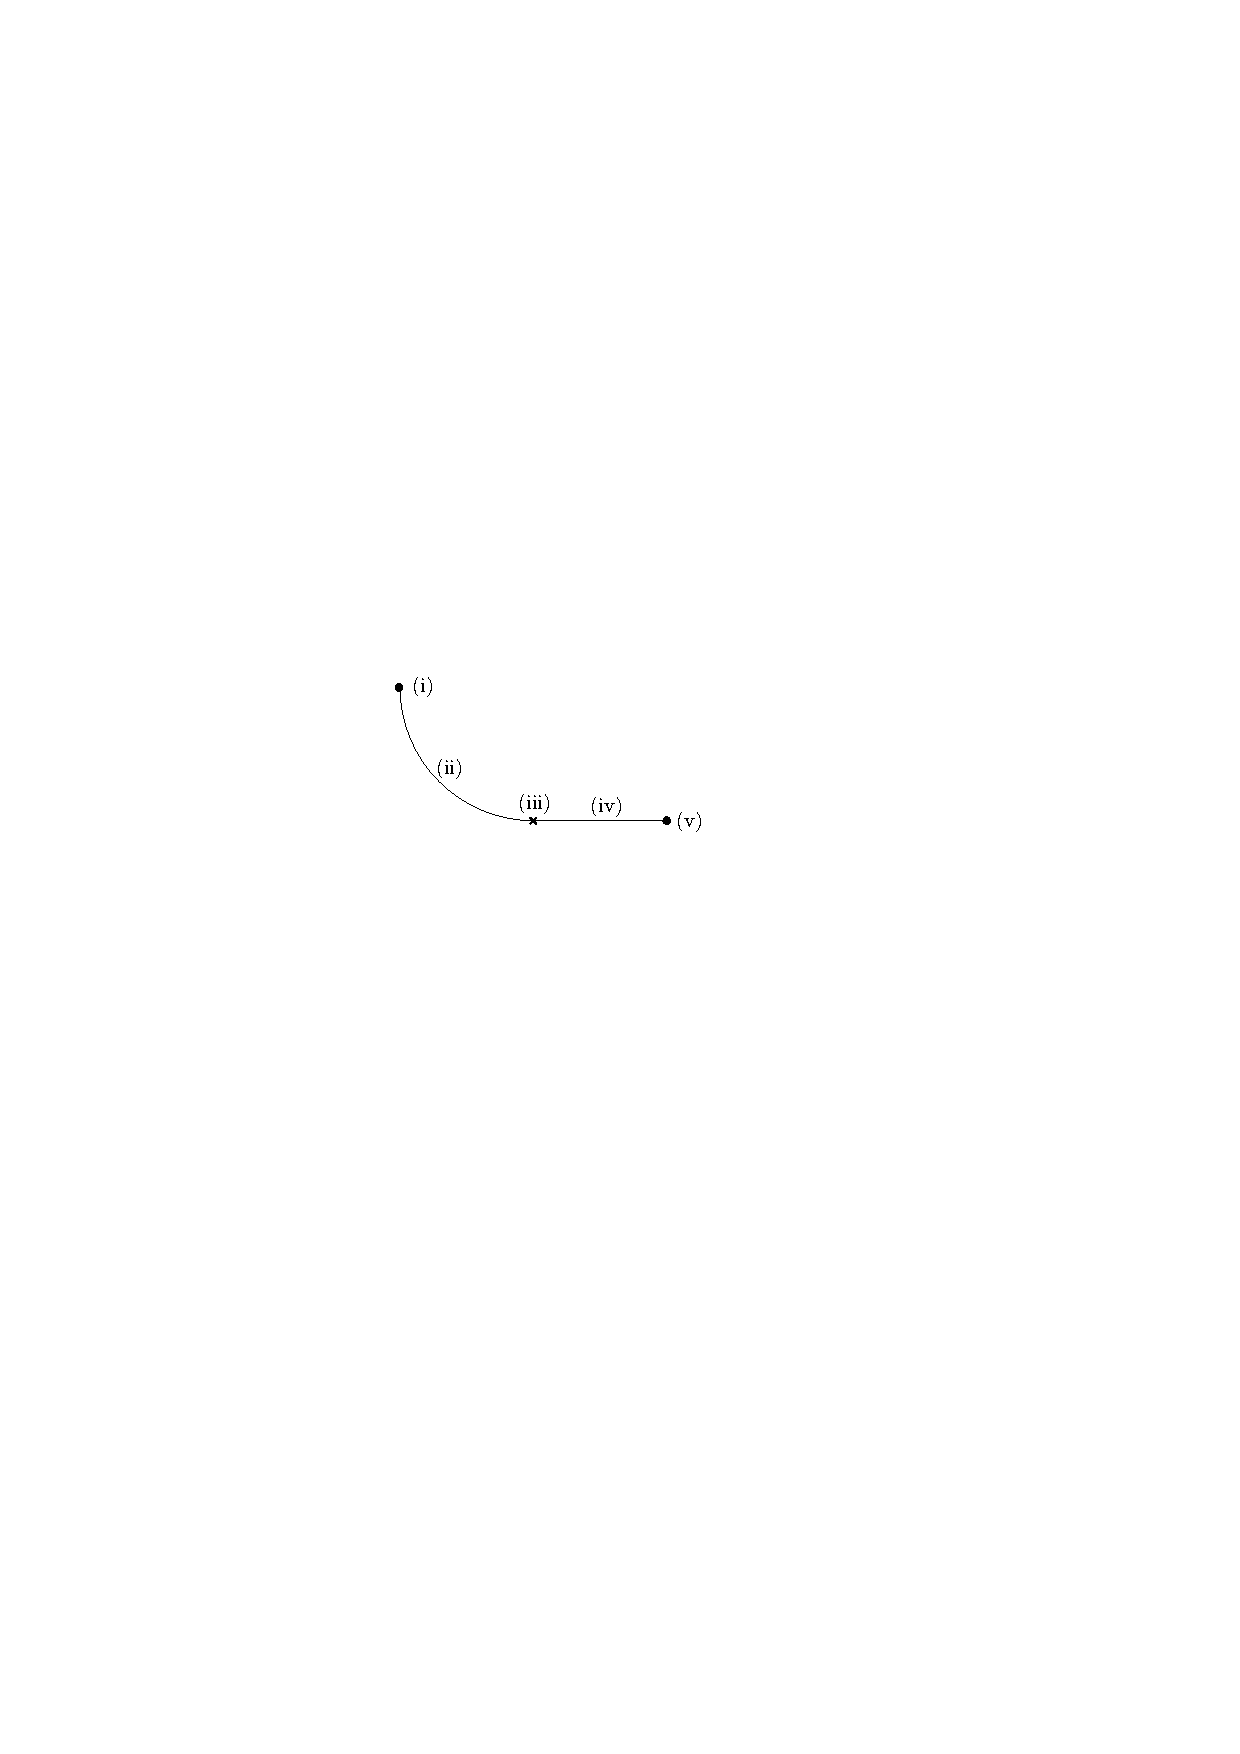
\includegraphics{anatomieLKante}
  \caption{Bezeichnungen in glatt"=orthogonalen Zeichnungen anhand der L"~Kante: (i) oberer Knoten, (ii) 90\textdegree-Kreissegment, (iii) Knick, (iv) horizontales Liniensegment, (v) unterer Knoten.}
  \label{fig:anatomieLKante}
\end{figure}

Zwei Beispiele für glatt"=orthogonale Zeichnungen finden sich in Abbildung~\ref{fig:exampleAsmooth}. In der Zeichnung~\ref{fig:exampleAsmoothSimple} fällt die lange Kante $\{0,4\}$ mit einem 270\textdegree-Kreissegment auf.

\begin{figure}[h]
  \centering
\begin{subfigure}[b]{0.3\textwidth}
  \centering
  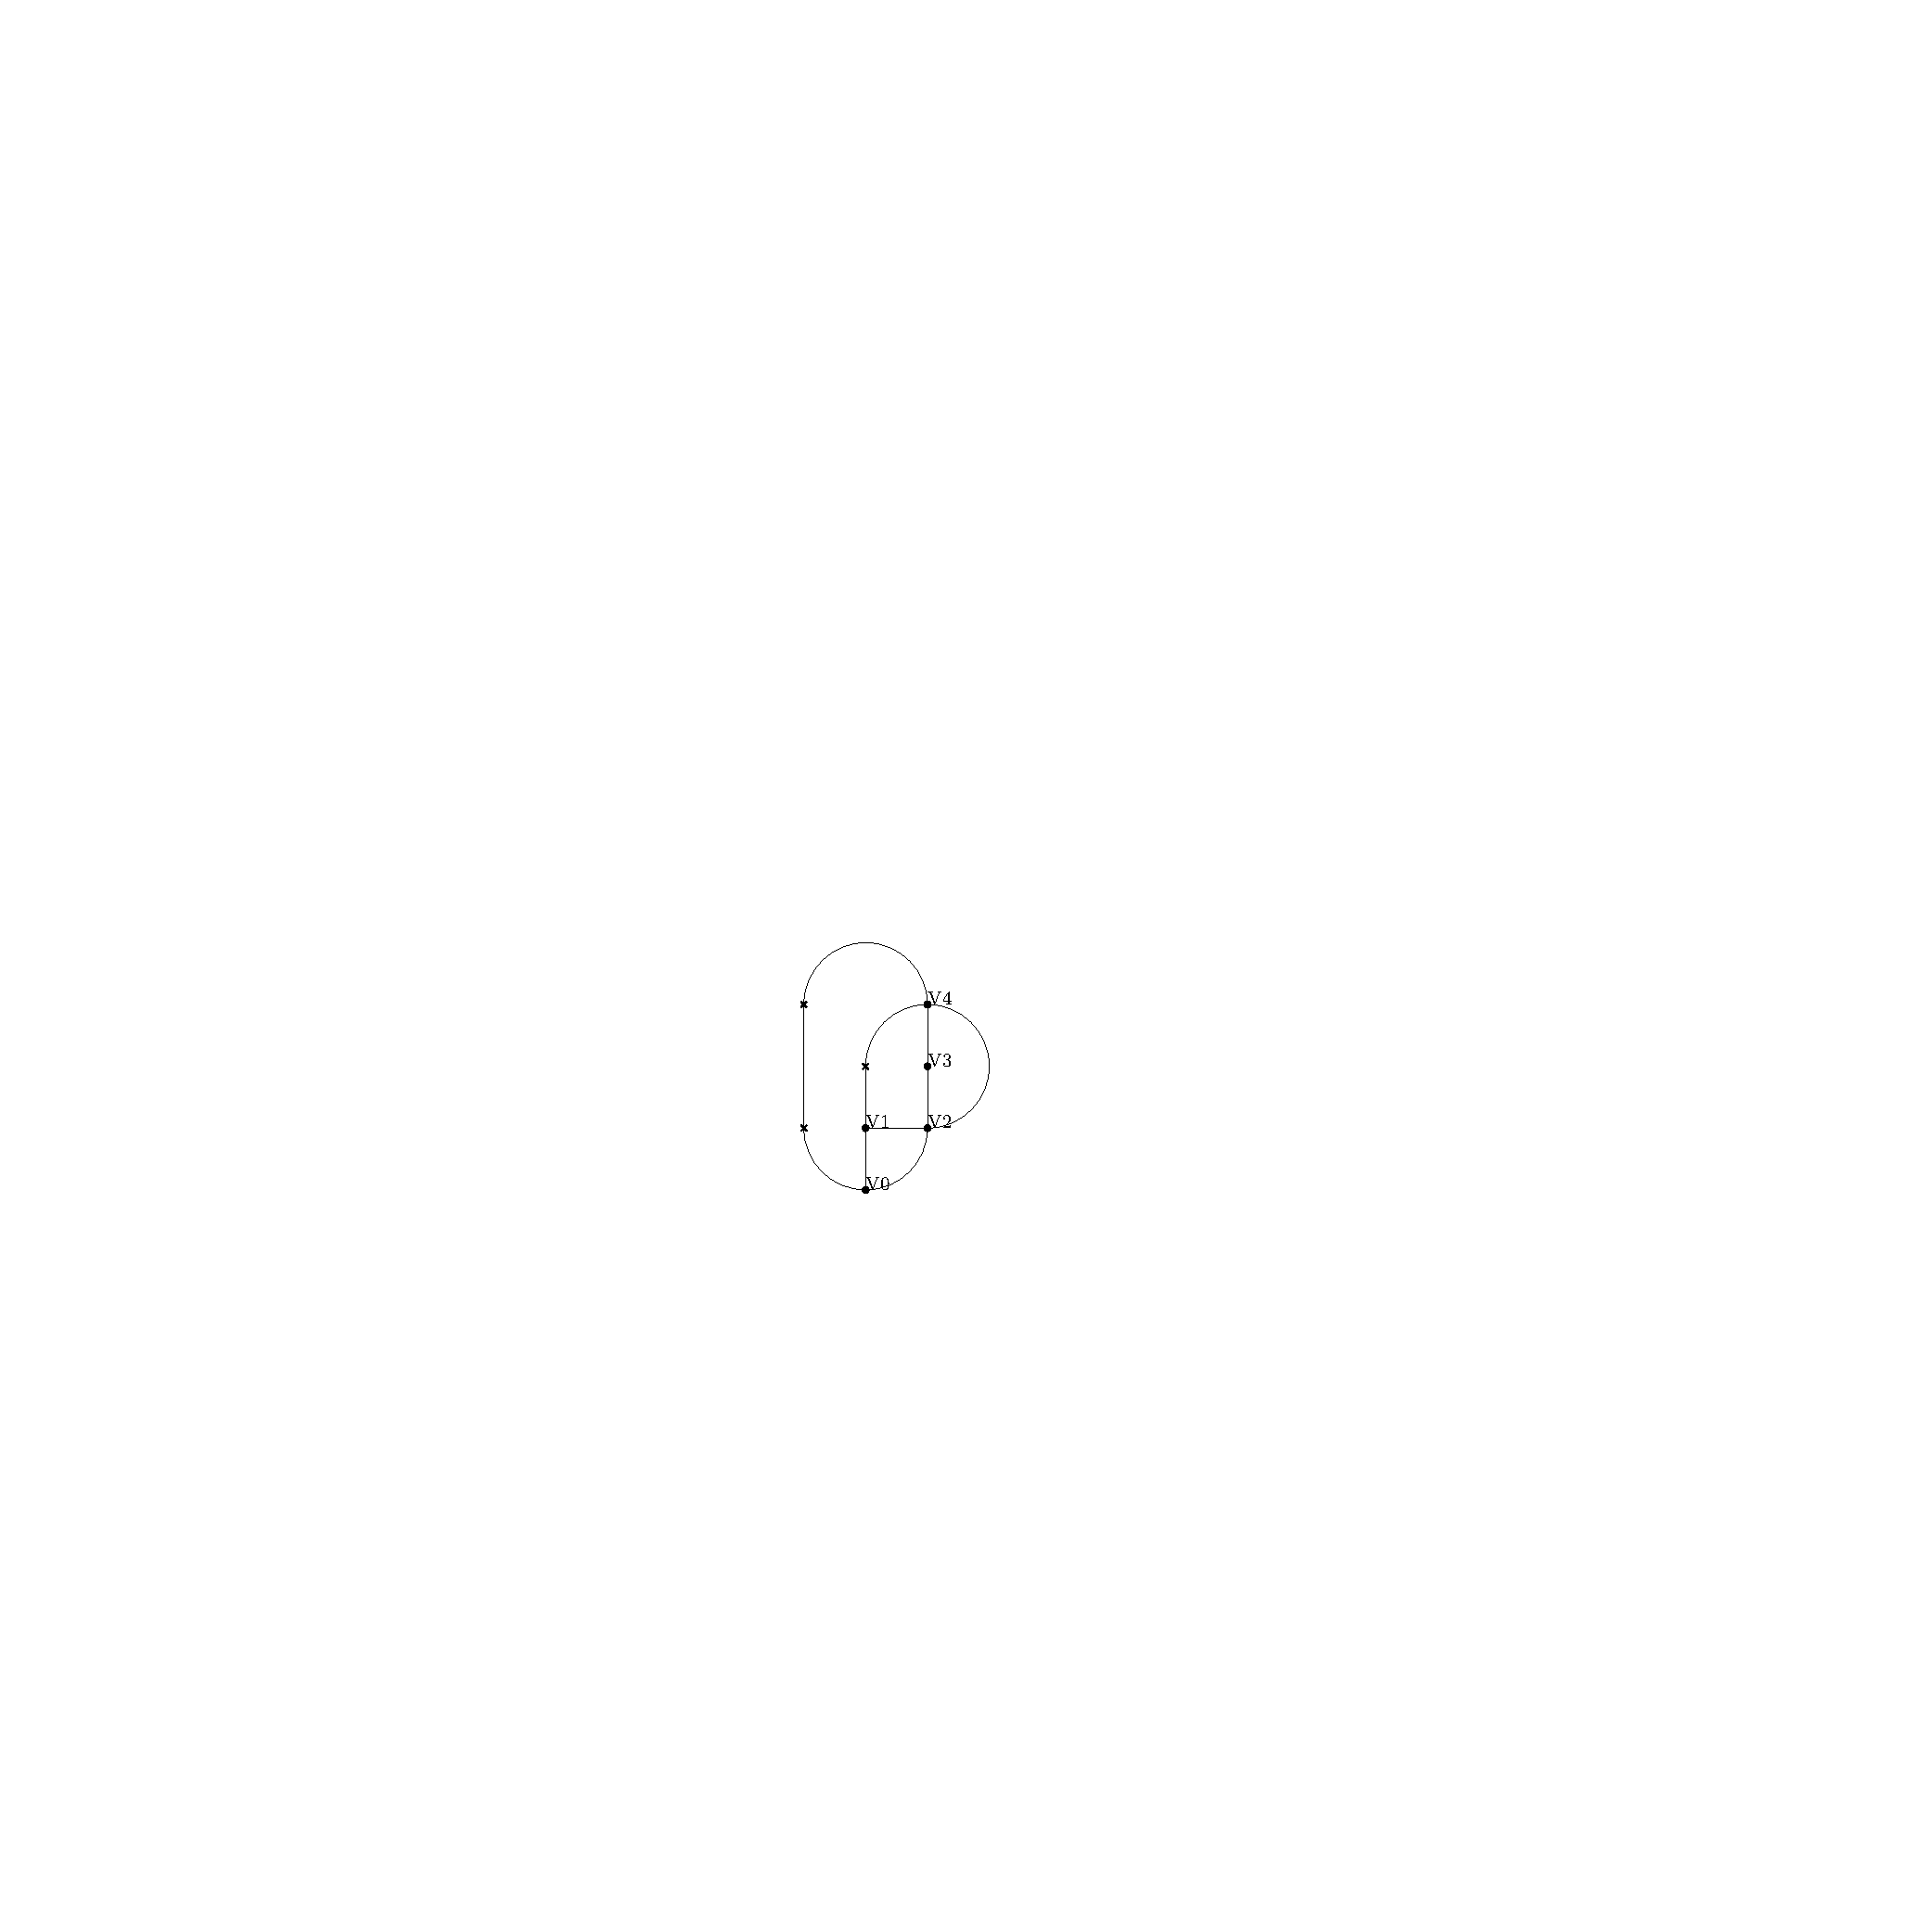
\includegraphics{exampleA/smoothComplex}
  \caption{Mit Kante $\{0,4\}$ aus drei Segmenten.}
  \label{fig:exampleAsmoothComplex}
\end{subfigure}
  \quad
\begin{subfigure}[b]{0.6\textwidth}
  \centering
  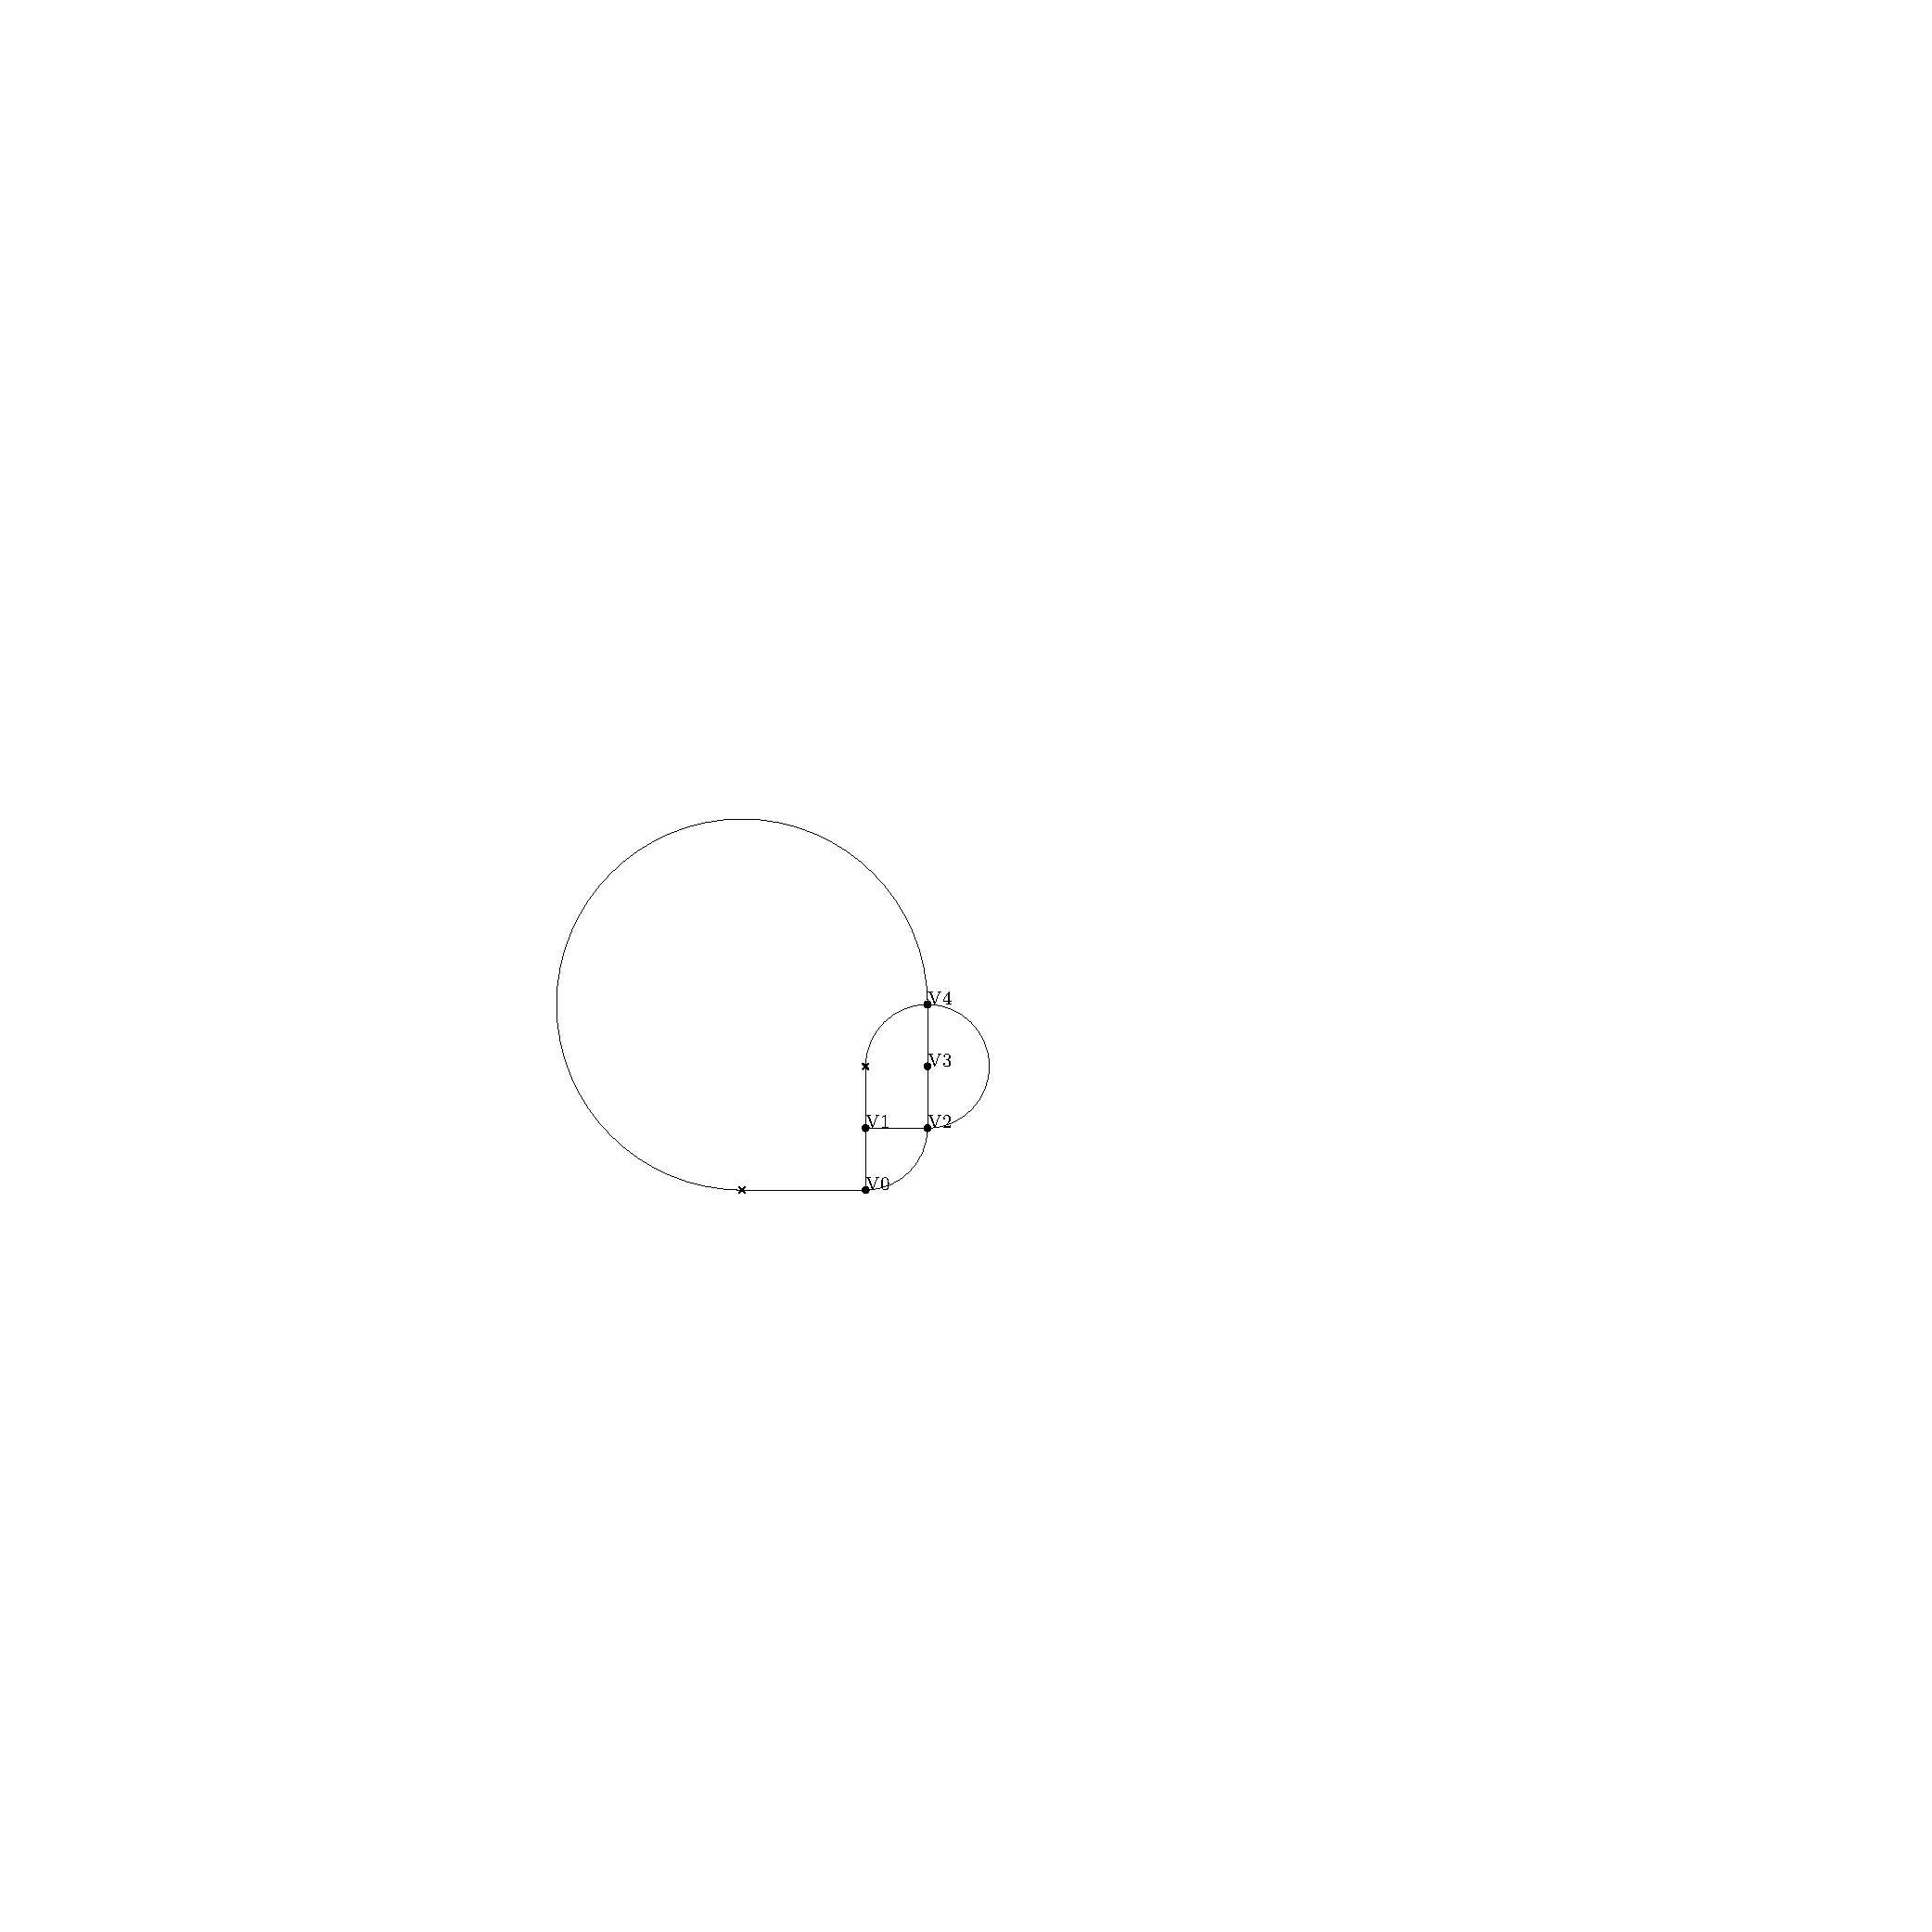
\includegraphics{exampleA/smooth}
  \caption{Mit Kante $\{0,4\}$ aus zwei Segmenten.}
  \label{fig:exampleAsmoothSimple}
\end{subfigure}
  \caption{Der Graph $G_\text{E}$ aus Beispiel~\ref{ex:graph} in zwei glatt"=orthogonalen Versionen der Zeichnung aus Abbildung~\ref{fig:exampleAorthogonalCompress}. Die Knickpunkte zwischen zwei Segmenten einer Kante sind als Kreuze eingezeichnet.}
  \label{fig:exampleAsmooth}
\end{figure}

Ebenso wie bei orthogonalen Zeichnungen gibt man die \emph{Komplexität} einer glatt"=ortho-gonalen Zeichnung in Abhängigkeit der größten Anzahl von Segmenten $k$ in einer Kante dieser Zeichnung an, und nennt sie dann eine \emph{$\text{SC}_k$-Zeichnung}. Ein triviale Umwandlung einer orthogonalen Zeichnung in eine glatt"=orthogonale Zeichnung wäre es, alle 90\textdegree-Knicke durch 90\textdegree-Kreissegmente mit dem Radius einer Gittereinheit zu ersetzen.

Konvertiert man die Kante $\{0,4\}$, wie sie in der OC$_3$-Zeichnung aus Abbildung~\ref{fig:exampleAorthogonalNocompress} zu sehen ist, auf diese Methode, erhielte man drei Segmente, zu sehen in der Zeichnung~\ref{fig:exampleAsmoothComplex}. Wäre das obere horizontale Segment etwas länger, erhielte man gar fünf Segmente, und somit wäre die resultierende Zeichnung von der Komplexität SC$_5$.

Benutzt man jedoch das große 270\textdegree-Kreissegment, schafft man es, die Anzahl der Segmente auf zwei zu reduzieren und man erhält eine SC$_2$-Zeichnung. Wir streben nun Zeichnungen mit möglichst niedriger Komplexität an. Es gibt nicht für alle 4"~planare Graphen eine SC$_1$-Zeichnung, und solche Zeichnungen haben u.U. einen vergleichsweise großen Platzbedarf. Eine SC$_2$-Zeichnung ist jedoch stets möglich, wie anhand des Algorithmus zu sehen ist. Auch sie haben im Allgemeinen einen größeren Platzbedarf als die SC$_5$-Zeichnung der trivialen Umwandlung, dies ist jedoch ein Kompromiss, der für die geringere Kantenkomplexität eingegangen werden muss. % TODO: Proof? Elaborate? idk

Auch für SC$_2$ Zeichnungen ist es sinnvoll, das Aussehen der Kanten so zu normieren, dass die Angabe der Knotenpositionen und der Ports eine Zeichnung vollständig beschreibt. Dies wird in Abschnit~\ref{sec:sc2conversion} weiter ausgeführt.




\chapter{Algorithmus}
\label{chap:algo}

Nachdem nun im Grundlagen-Kapitel~\ref{chap:basics} die nötigen Begriffe definiert wurden, und darauf hingeführt wurde, welche Probleme der Algorithmus lösen muss und welche nicht, wird nun in diesem Kapitel der Algorithmus Schritt für Schritt erklärt.

\section{Übersicht}

Der Algorithmus erhält als Eingabe einen 4"~planaren, zweifach knotenzusammenhängenden Graphen. Die Ausgabe ist eine glatt"=orthogonale SC$_2$ Zeichnung des Graphen. Der Algorithmus berechnet als Voraussetzung eine planare Einbettung und eine $st$-Ordnung für den Graphen. Damit eine Einbettung berechnet werden kann, muss der Graph planar sein. Die fertige Zeichnung wird die hier berechnete Einbettung widerspiegeln. Die planare Einbettung muss lediglich konsistente Sortierungen für die Adjazenzlisten liefern, ansonsten kann sie frei bestimmt werden. Aus der planaren Einbettung wird später die Reihenfolge der Kanten bei der Portzuweisung festgelegt.

Damit eine $st$-Ordnung berechnet werden kann, muss der Graph zweifach zusammenhängend sein. Der Unteralgorithmus zur Berechnung der $st$-Ordnung muss als Eingabe zwei Knoten $s$ und $t$ akzeptieren, die als Quelle und Senke verwendet werden. Die beiden Knoten müssen an dieselbe Facette grenzen. Diese wird in der Zeichnung die Außenfacette werden. Soll also eine bestimmte Facette die äußere werden, können die beiden Knoten entsprechend gewählt werden. Die resultierende $st$-Ordnung gibt die Reihenfolge an, in der die Knoten im nächsten Schritt platziert werden. Auf Grundlage der $st$-Ordnung und der planaren Einbettung wird nun in drei Iterationen ein Layout als Vorgabe für die Zeichnung berechnet. 

Die erste Iteration erstellt ein orthogonales Layout für eine OC$_3$-Zeichnung. Es behält die planare Einbettung bei und platziert die Knoten in der von der st-Ordnung vorgegebenen Reihenfolge. Die hier festgelegten Portzuweisungen werden nun nicht mehr verändert, lediglich die Positionen der Knoten werden in den nächsten beiden Iterationen angepasst.

In der zweiten Iteration wird dieses Layout so verkleinert, dass stufenförmige Kanten zu horizontalen Linien konvertiert werden. Während vorher alle Knoten eine unterschiedliche Höhe, also y"~Koordinaten, hatten, werden nun mehrere Knoten platzsparend auf einer Höhe untergebracht.

In der dritten Iteration wird das Layout für die OC$_3$-Zeichnung so angepasst, dass es auch als Layout für eine planare SC$_2$-Zeichnung dienen kann. Würde man direkt die glatt"=orthogonalen Kanten einzeichnen, wäre die entstandene Zeichnung in vielen Fällen nicht planar. Darum müssen die Knoten so auseinandergezogen werden, dass genug Platz für die Kanten ist und sie überschneidungsfrei verlaufen, aber nicht gleichzeitig andere Kanten so verändert werden, dass sie wiederum neue Überschneidungen bilden.

Wenn das Layout für die SC$_2$-Zeichnung fertig ist, bleibt nur noch als letzter Schritt, aus dem Layout eine Zeichnung herzustellen. Dazu muss aus den Portzuweisungen und den Positionen der Knoten relativ zueinander auf die Formen der Kanten geschlossen werden.

Nach Abschluss des letzten Schrittes erhält man eine glatt"=orthogonale SC$_2$-Zeichnung des 4"~planaren, zweifach knotenzusammenhängenden Graphen. Die Schritte sind in Algorithmus~\ref{alg:biconnected} zusammengefasst.

\begin{algorithm}[ht]
  \SetKw{True}{true}
  \SetKw{False}{false}
  \caption{SmoothOrthogonalDrawBiconnected(Graph $G = (V,E)$)}
  \label{alg:biconnected}
  \Ein{4-planarer, zweifach knotenzusammenhängender Graph $G = (V,E)$}
  \Aus{SC$_2$-Layout von $G$}
  
  $\Epsilon \leftarrow$ CalculatePlanarEmbedding$(G)$ \;
  Wähle zwei Knoten $s, t \in V$ die in $\Epsilon$ an einer Facette liegen.\;
  $St \leftarrow$ CalculateStOrdering$(G, s, t)$ \;
  $O \leftarrow$ GenerateOrthogonalLayout$(G,St,\Epsilon)$ \;
  $O' \leftarrow$ EliminateS-Shapes$(O)$ \;
  $O'' \leftarrow$ EliminateCrossings$(O')$ \;
  $\Gamma \leftarrow$ DrawSmoothOrthogonalLayout$(O'')$ \;
  
  \Return $\Gamma$
\end{algorithm}

\section{Orientierte Graphen und Tiefensuche}

Eine algorithmische Grundlage, die im Verlauf des Algorithmus mehrmals verwendet wird, ist die \emph{Tiefensuche}. Sie wurde von Tarjan~\cite{tarjan-72} formalisiert. Konträr zum Namen werden jedoch oft keine Knoten gesucht, sondern vielmehr ein Tiefensuchenbaum konstruiert.

Bei der Tiefensuche wird der Graph orientiert. Ein \emph{orientierter Graph} eines Graphen $G = (V, E)$ weist den Knoten jeder Kante eine Reihenfolge zu. Jede Kante $e \in E$ ist also ein geordnetes Paar $e = (v_\text{A}, v_\text{B})$ und die Kanten bekommen damit eine Richtung, sie zeigen von $v_\text{A}$ nach $v_\text{B}$. Man nennt $v_\text{A}$ \emph{Vorgänger} von $v_\text{B}$ und $v_\text{B}$ heißt Nachfolger von $v_\text{A}$. Die Kante ist eine \emph{ausgehende Kante} von $v_\text{A}$ und eine \emph{eingehende Kante} von $v_\text{B}$. Die Anzahl der ausgehenden Kanten eines Knotens heißt sein \emph{Ausgangsgrad}, analog gibt es den \emph{Eingangsgrad}.

Schon aus einer $st$-Ordnung könnte ein orientierter Graph gewonnen werden, indem die Kanten von einem Knoten mit höherer Zahl zu einem mit niedrigerer orientiert werden. Die Tiefensuche liefert eine andere Orientierung.

Im Verlauf der Tiefensuche nach Algorithmus~\ref{alg:dfs} wird nicht nur ein orientierter Graph berechnet, jedem Knoten wird eine \emph{Auffindungszeit} zugewiesen, und eine Partition der Kanten $E = E_\text{T} \cup E_\text{R}$ wird erstellt. Man nennt die Kanten $e_\text{T} \in E_\text{T}$ \emph{Baumkanten} und die übrigen Kanten $e_\text{R} \in E_\text{R} =  E \setminus E_\text{T}$ \emph{Rückwärtskanten}. Die Baumkanten zeigen jeweils von einem Knoten mit niedrigerer Auffindungszeit zu einem mit höherer. Die Startknoten, die \emph{Wurzeln}, haben keine eingehende Baumkante, jeder andere Knoten hat genau eine. Die Rückwärtskanten zeigen jeweils von einem Knoten mit höherer Auffindungszeit zu einem mit niedrigerer. Das Tupel der beiden Mengen von gerichteten Kanten $(E_T, E_R)$ nennen wir \emph{Tiefensuchenbaum}, bei Tarjan~\cite{tarjan-72} heißt es \emph{palm tree}.

Im Algorithmus~\ref{alg:dfs} sind die Knoten, die in Zeile~\ref{alg:dfs:nl:connectedStart} behandelt werden, Wurzeln. In Zeile~\ref{alg:dfs:nl:treeEdge} wird eine Kante orientiert und als Baumkante kategorisiert, in Zeile~\ref{alg:dfs:nl:backEdge} als Rückwärtskante.

\begin{algorithm}[ht]
  \SetKw{True}{true}
  \SetKw{False}{false}
  \SetKwBlock{Visit}{Visit(v)}{end}
  \caption{BuildPalmTree(Graph $G = (V,E)$)}
  \label{alg:dfs}
  \Ein{ungerichteter Graph $G = (V,E)$}
  \Aus{Tiefensuchenbaum $(E_T, E_R)$ von $G$}
\BlankLine
  $E_T \leftarrow \emptyset$, $E_R \leftarrow \emptyset$ \;
  \For{$v \in V$}{
    $v$.discoveryTime $\leftarrow \perp$ \;
  }
  $i := 0$ \;
\BlankLine
  \For{$v \in V$}{
    \If{$v$.discoveryTime == $\perp$}{
      Visit$(v)$ \; \nllabel{alg:dfs:nl:connectedStart}
    }
  }
\BlankLine
  \Visit{
    $v$.discoveryTime $\leftarrow i$ \; \nllabel{alg:dfs:nl:visitStart}
    $i \leftarrow i+1$ \;
    \For{$w \in A(v)$}{
      \If{$w$.discoveryTime == $\perp$}{ \nllabel{alg:dfs:nl:decide}
        $E_T \leftarrow E_T \cup \{(v, w)\}$ \; \nllabel{alg:dfs:nl:treeEdge}
        Visit(w) \; \nllabel{alg:dfs:nl:recur}
      }
      \Else{
        \If{$w$.discoveryTime < $v$.discoveryTime {\bf and}  $(v, w) \notin E_T$}{
          $E_R \leftarrow E_R \cup \{(v, w)\}$\; \nllabel{alg:dfs:nl:backEdge}
        }
      }
    }
  }
\BlankLine
    \Return\{$(E_T, E_R)$\}
\end{algorithm}

Die Tiefensuche ist so grundlegend für viele der kommenden Algorithmen, da sie zu mehr als der Berechnung eines Tiefensuchenbaums verwendet werden kann, indem man entsprechende Zeilen einfügt. 

Beispielsweise können die Zusammenhangskomponenten eines Graphen bestimmt werden, da jedes Mal, wenn Zeile \ref{alg:dfs:nl:connectedStart} erreicht wird, alle folgenden Knoten zu einer neuen Zusammenhangskomponente gehören. Ist ein Graph zusammenhängend, gibt es somit nur eine Wurzel.

Die Höhe eines Knotens im Tiefensuchenbaum ist die Länge des Weges von Baumkanten von der Wurzel zum Knoten. Sie kann im Verlauf der Tiefensuche mit abgespeichert werden, indem man vor Zeile~\ref{alg:dfs:nl:connectedStart} die Anweisung $v.$height $\leftarrow 0$ einfügt, und vor Zeile~\ref{alg:dfs:nl:recur} die Anweisung $w.$height $\leftarrow v.$height$ + 1$.


Für die Bestimmung von Zweifach-Zusammenhangskomponenten benötigt man das Konzept des \emph{Rückwegs}: Von einem Knoten $v$ kann man den Baumkanten zu Knoten mit höherer Auffindungszeit folgen. Von diesen Knoten können Rückwärtskanten ausgehen, die mitunter zu Knoten mit einer kleineren Auffindungszeit als der von $v$ führen. Den Knoten mit der niedrigsten Auffindungszeit, den wir auf diese Weise vom Knoten $v$ erreichen können, nennen wir \emph{Rückpunkt}. Hat ein Knoten sich selbst als Rückpunkt, kann also kein niedrigerer Knoten erreicht werden, so ist er Trenner von Zweifach-Zusammenhangskomponenten.

Die Rückpunkte können während der Tiefensuche bestimmt werden. Wenn ein Knoten $v$ besucht wird, also in Zeile~\ref{alg:dfs:nl:visitStart}, wird der Knoten $v$ selbst als Rückpunkt gespeichert. Wird in Zeile~\ref{alg:dfs:nl:backEdge} eine Rückwärtskante von $v$ nach $w$ gefunden, so wird geprüft, ob $w$ niedriger ist als der bisherige Rückpunkt von $v$ und, wenn ja, wird der Rückpunkt von $v$ auf $w$ gesetzt. Nach der Rückkehr vom rekursiven Aufruf in Zeile~\ref{alg:dfs:nl:recur} wird geprüft, ob der Knoten $w$ nun einen echt niedrigen Rückpunkt als $v$ hat, wenn ja, wird der Rückpunkt von $v$ auf den Rückpunkt von $w$ gesetzt. Beim Berechnen der planaren Einbettung und der st-Ordnung werden Rückpunkte und Rückwege verwendet.

\section{Bestimmung einer planaren Einbettung}

Da am Ende eine planare Zeichnung entstehen soll, wird zuerst eine planare Einbettung berechnet. Hierbei wird auch geprüft, ob der Graph überhaupt planar ist, d.h. ob es möglich ist, eine planare Einbettung zu erstellen. 

Zum Prüfen auf Planaritätseigenschaft gibt es diverse Algorithmen, die bei Patrignani~\cite{patrignani-07} vorgestellt und verglichen werden. Der erste effiziente Linearzeit-Algoritmus wurde von Hopcroft und Tarjan~\cite{hopcroft+tarjan-74} veröffentlicht, jedoch ist er sehr schwer zu implementieren, somit wurde für die Implementierung nach einer Alternative gesucht. Dass dann der Links-Rechts-Planaritätstest wie von Brandes~\cite{brandes-09} beschrieben ausgewählt wurde, begründet sich mit zweierlei Abwägungen. Zum einen ist es wichtig, dass nicht nur die Planarität getestet wird, sondern auch eine planare Einbettung angegeben werden kann, damit diese für das Zeichnen zur Verfügung steht. Dies wurde bei \cite{brandes-09} mittels vergleichsweise geringem Aufwand realisiert. Zum anderen liefert \cite{brandes-09} eine Beschreibung, die eine Implementierung begünstigt, da zu den Schritten sehr detaillierter Pseudocode angegeben wird. % TODO: citations like this?

Für den Planaritätstest wird ein Tiefensuchenbaum $(E_T, E_R)$ des Eingabegraphen benötigt. Die Grundidee ist es, die Rückwärtskanten aus $E_\text{R}$ in zwei disjunkte Teilmengen $L$ und $R$, für Links und Rechts, einzuteilen. Betrachten wir nun einen Knoten $v \in V$ und zwei Baumkanten $(v, v_1), (v, v_2) \in E_T$. Nun sollen alle Kanten, die am Ende eines Rückwegs von $v_1$ aus liegen und echt höher enden als der Rückpunkt von $v_2$ zu einer Teilmenge gehören. Gleichzeitig sollen alle Kanten, die am Ende eines Rückwegs von $v_2$ aus liegen und echt höher enden als der Rückpunkt von $v_1$, zur jeweils anderen Teilmenge gehören. Der Graph ist genau dann planar, wenn eine solche Partition möglich ist. Die planare Einbettung erhält man, wenn man die Baumkanten hinzu nimmt und geeignet mit den Rückwärtskanten in eine Reihenfolge der Adjazenzliste bringt.

Die so bestimmten geordneten Adjazenzlisten werden dann beim Erstellen des Layouts für die OC$_3$-Zeichnung verwendet.

\section{Ermitteln einer $st$-Ordnung}

Neben dem Graphen selbst und der planaren Einbettung benötigt der Schritt, in dem das OC$_3$-Layout erstellt wird, eine st-Ordnung, eine Reihenfolge der Knoten $v_1, \dots, v_n$, mit $s=v_1$ und $t=v_n$, in der die Knoten dann platziert werden. 

Jeder Knoten, außer $s$ und $t$, soll mindestens einen Nachbarn mit einem höheren Index und mindestens einen mit einem niedrigeren Index haben. Da die Indizes paarweise verschieden sind, erhalten wir zudem einen orientierten Graphen, wenn wir die ungerichteten Kanten so ausrichten, dass sie vom niedrigeren Index zum höheren verlaufen.

Die $st$-Ordnung soll mit der planaren Einbettung kompatibel sein, d.h. wir wählen zwei Knoten $s$ und $t$ auf der Außenfacette. Damit haben wir eine günstige Reihenfolge für die Platzierung der Knoten bei der Berechnung des Layouts. 

Eine solche $st$-Ordnung lässt sich mit einer angepassten Tiefensuche und einer passenden Nachbearbeitung für jeden zweifach zusammenhängenden Graphen ermitteln. Ein Beweis in Form eines Linearzeit-Algorithmus findet sich bei Even und Tarjan~\cite{even+tarjan-75}, basierend auf vorherigen Resultaten (\cite{hopcroft+tarjan-74},~\cite{tarjan-72}).

Die Tiefensuche wird so angepasst, dass jedes Mal, wenn wir den Rückpunkt eines Knotens $v$ aktualisieren, die aktuelle Kante als zugehörig zum Rückweg des Knotens $v$ gespeichert wird. Außerdem beginnt die Tiefensuche mit der Kante $\{s, t\}$.

Der Nachbearbeitungsschritt speichert zu jeder Kante und jedem Knoten, ob sie/""er schon abgearbeitet wurde. Er fügt die Knoten in der Reihenfolge der $st$-Ordnung zu einer Ergebnisliste hinzu. Er legt dazu $t$ unter $s$ auf einen Stack. Solange der Stack nicht leer ist, wird wiederholt ein Knoten $v$ herunter genommen. Es wird nun ein Pfad vom Knoten $v$ aus gesucht, der noch nicht abgearbeitete Kanten benutzt, um zu einem bereits abgearbeiteten Knoten zu gelangen. Wird so ein Pfad gefunden, so werden die Knoten entlang des Pfades auf den Stack gelegt, ganz unten der vorletzte Knoten des Pfades bis zuletzt ganz oben $v$ abgelegt wird. Wird kein solcher Pfad gefunden, so wird $v$ an die Ergebnisliste angehängt und ist nun nicht mehr auf dem Stack.

Für das Finden eines Pfades gibt es drei Möglichkeiten, die der Reihe nach ausprobiert werden. Gibt es eine nicht abgearbeitete, ausgehende Rückwärtskante, so ist diese der Pfad. Gibt es ansonsten eine nicht abgearbeitete Baumkante, so wird dieser gefolgt und dann dem Rückweg des Zielknotens, bis er auf einen abgearbeiteten Knoten trifft. Gibt es nur noch eine nicht abgearbeitete eingehende Rückwärtskante, so wird dieser gefolgt und dann den Baumkanten zurück bis zu einem abgearbeiteten Knoten. Die Knoten und Kanten des Pfades werden als abgearbeitet markiert. Gibt es nur noch abgearbeitete Kanten, wird kein Weg gefunden.

Zuletzt stehen in der Ergebnisliste die Knoten in der Reihenfolge einer $st$-Ordnung.

\section{Erstellung eines OC$_3$-Layouts}
\label{sec:oc3algo}

In den vorausgegangenen Schritten wurden zum einen die Knoten in die Reihenfolge einer $st$-Ordnung $v_1, \dots, v_n$ gebracht, wobei $s = v_1$ und $t = v_n$, und zum anderen die Adjazenzlisten im Sinne einer planaren Einbettung sortiert. Außerdem wurde die Facette, auf der die Knoten $s$ und $t$ liegen, als Außenfacette eingeplant. Mit diesen Informationen wird nun ein geeignetes OC$_3$-Layout für den zweifach zusammenhängenden 4"~planaren Graphen erstellt. 

Da am Ende die Komplexität der glatt"=orthogonalen Kanten gering sein soll, bietet es sich an, bereits ein orthogonales Layout mit niedriger Komplexität zu erstellen. Dazu wird der Algorithmus verwendet, der sich bei Liu et al.~\cite{liu+etal-98} und bei Biedl~\& Kant \cite{biedl+kant-98} findet. Die grundlegenden Ideen sind weitestgehend gleich, die beiden Beschreibungen wurden jedoch unabhängig voneinander entwickelt und unterscheiden sich teils deutlich, Biedl~\& Kant wenden das Verfahren zusätzlich auf nicht-planare Graphen an. Daher soll hier noch einmal der Algorithmus beschrieben werden, wie er für die Zwecke dieser Arbeit implementiert wurde. Es wird damit gezeigt, dass für jeden zweifach zusammenhängenden 4"~planaren Graph ein OC$_3$-Layout erstellt werden kann.

Das Resultat besteht nach Definition~\ref{def:layouts} aus der Portzuweisung $P: \{(v, e) \in V \times E \mid v \in e\} \to \{\text{L, R, T, B}\}$ und den Layouts für die Kanten~$L_E$ und die Knoten~$L_V$.

Während die Portzuweisung und die x"~Koordinaten im Verlauf des Algorithmus bestimmt werden, werden die y"~Koordinaten direkt festgelegt: Die y"~Koordinate jedes Knotens~$v_i$ ist seine Nummer~$i$ in der $st$-Ordnung, die y"~Koordinate jeder Kante $e = (v_i, v_k)$, geordnet durch die Orientierung der $st$-Ordnung, ist die kleinere der beiden y"~Koordinaten~$i$ ihrer beiden Knoten.

Da sich x"~Koordinaten sonst häufig ändern würden, wird den Knoten und Kanten in der Platzierungsphase nur eine Spalte zugeordnet. So kann eine neue Spalte zwischen zwei bestehenden Spalten eingefügt werden, ohne die Koordinaten sämtlicher Knoten in den Spalten zu verändern. Am Anfang wird eine Referenzspalte erstellt. Erst nach Ablauf des Algorithmus werden die x"~Koordinaten auf Basis der Spalten festgelegt. Die Spalte einer Kante steht für die Position ihres horizontalen Segments.

\subsection{Schleife}

Der Algorithmus bearbeitet nun in einer Schleife die Knoten in der Reihenfolge der $st$-Ordnung.

Es wird die Schleifeninvariante eingehalten, dass, bevor Knoten~$v_i$ bearbeitet wird, die Knoten $v_1, \dots, v_{i-1}$ bereits in einer Spalte platziert sind und ihre Portzuweisungen vollständig berechnet wurden. Ebenso sind die Kanten zwischen diesen Knoten bereits in einer Spalte platziert. Die Kanten, die von einem der Knoten $v_1, \dots, v_{i-1}$ ausgehen, aber bei einem noch nicht platzierten Knoten $v_i, \dots, v_n$ enden, nennen wir \emph{offene Kanten}. Auch sie sind bereits in einer Spalte platziert.

Die Bearbeitung des Knotens~$v_i$ sorgt nun dafür, dass die Invariante für $v_{i+1}$ erfüllt ist. Dazu werden zuerst die Kanten an $v_i$ nach einem festgelegten Verfahren in Übereinstimmung mit der planaren Einbettung auf die Ports verteilt. Hat der Knoten nun eine Kante am unteren Port, so wird er in die Spalte der Kante an diesem unteren Port platziert. Hat er keine Kante am unteren Port, so ist es der Knoten~$s = v_1$, und er wird in die Referenzspalte platziert. Danach wird noch den, nach der Orientierung der $st$-Ordnung, ausgehenden Kanten des Knotens eine Spalte zugewiesen. Somit ist die Invariante für $v_{i+1}$ erfüllt.

Am Ende der Schleife, wenn die Invariante für $t = v_n$ erfüllt ist, sind alle Kanten und Knoten platziert und die Portzuweisung ist vollständig berechnet. Zudem hat die resultierende Zeichnung die gegebene planare Einbettung.

Um die Beschreibung zu vervollständigen, muss noch ausgeführt werden, wie die Ports an einem Knoten zugewiesen werden und wie die offenen Kanten platziert werden. Insbesondere muss jeder Knoten, außer $s$, eine Kante am unteren Port erhalten, damit er in eine Spalte platziert werden kann.

\subsection{Portzuweisung}
\label{sec:portdistribution}

Für die Portzuweisung wird die Ajdazenzliste partitioniert. Da der Graph maximal Grad~4 hat, ist die Größe der Adjazenzliste maximal~4. Durch die $st$-Ordnung erhalten wir eine Orientierung des Graphen und somit eingehende und ausgehende Kanten am Knoten. Die planare Einbettung hat die Adjazenzliste vorsortiert. Wir können daher die Adjazentliste in eine Liste von eingehenden und eine Liste von ausgehenden Kanten teilen. Die ein- und ausgehenden Kanten werden dann getrennt den Ports zugewiesen. Hier ergibt sich ein Speziallfall: Da es an $v_1$ nur ausgehende Kanten, und an $v_n$ nur eingehende Kanten gibt, könnte jede Kante die erste Kante in der Liste der aus- bzw.\ eingehenden Kanten sein. Hier wird die Liste so rotiert, dass die erste und die letzte Kante die beiden Kanten der Außenfacette sind.

Für die eingehenden Kanten werden, wie in Abbildung~\ref{fig:embedin} gezeigt, je nach Eingangsgrad des Knotens folgende Ports zur Verwendung ausgewählt: unten (Eingangsgrad~1 bis~4), links (2--4), rechts (3,4), oben (4). Der obere Port wird also nur bei Eingangsgrad~4 verwendet, was nur bei der Senke~$v_n$ vorkommen kann. Bei Eingangsgrad~0 müssen keine eingehenden Kanten behandelt werden, was nur bei der Quelle $v_1$ vorkommt. In allen anderen Fällen wird der untere Port einer Kante zugeordnet. Somit hat jeder Knoten außer $v_1$ eine Kante an seinem unteren Port. Den zur Verwendung ausgewählten Ports werden dann die eingehenden Kanten nach der Reihenfolge der planaren Einbettung im Uhrzeigersinn, beginnend bei rechts, dann unten und links, zuletzt oben, zugewiesen.

\begin{figure}[h]
        \centering
        \subcaptionbox{0\label{fig:embedindeg0}}
            {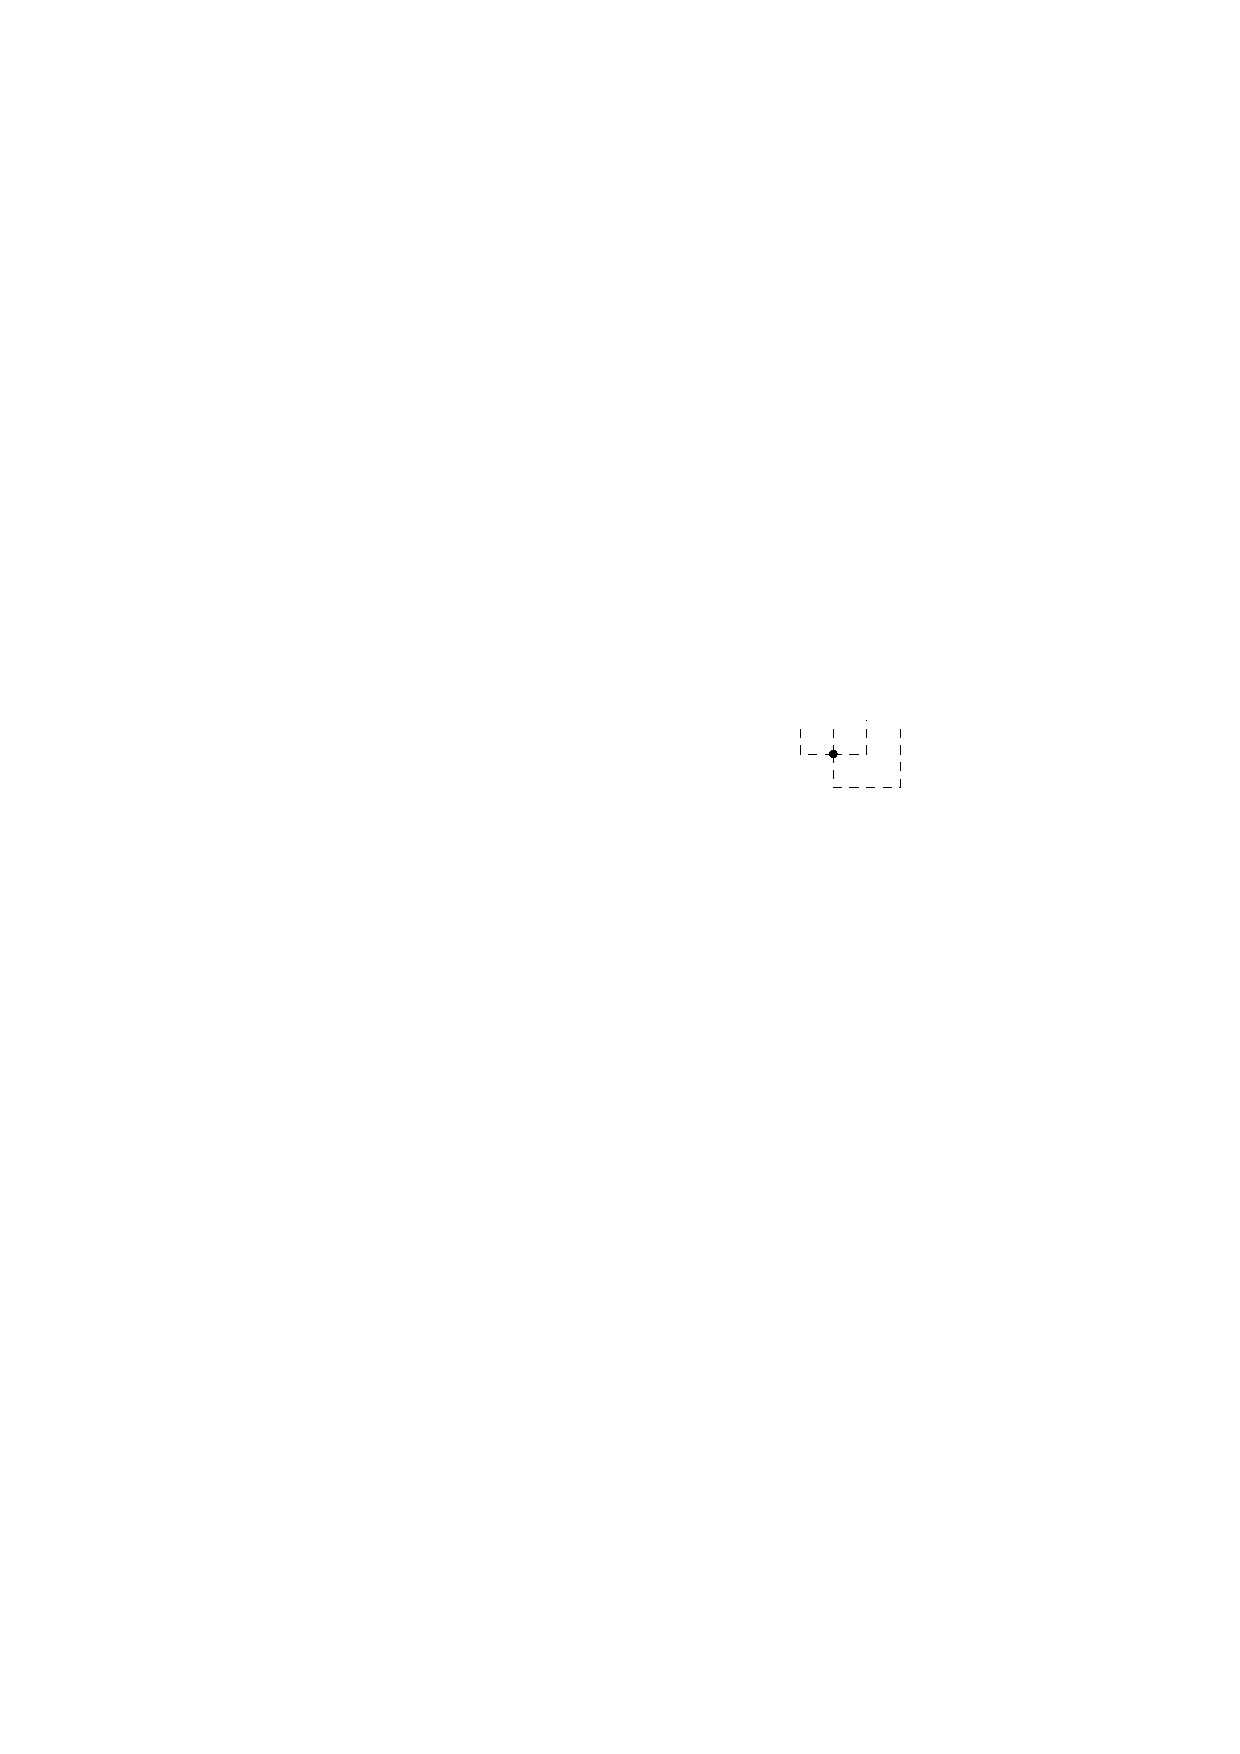
\includegraphics[scale=.8]{oc3_embed/incoming/indeg0}}
        \quad
        \subcaptionbox{1\label{fig:embedindeg1}}
            {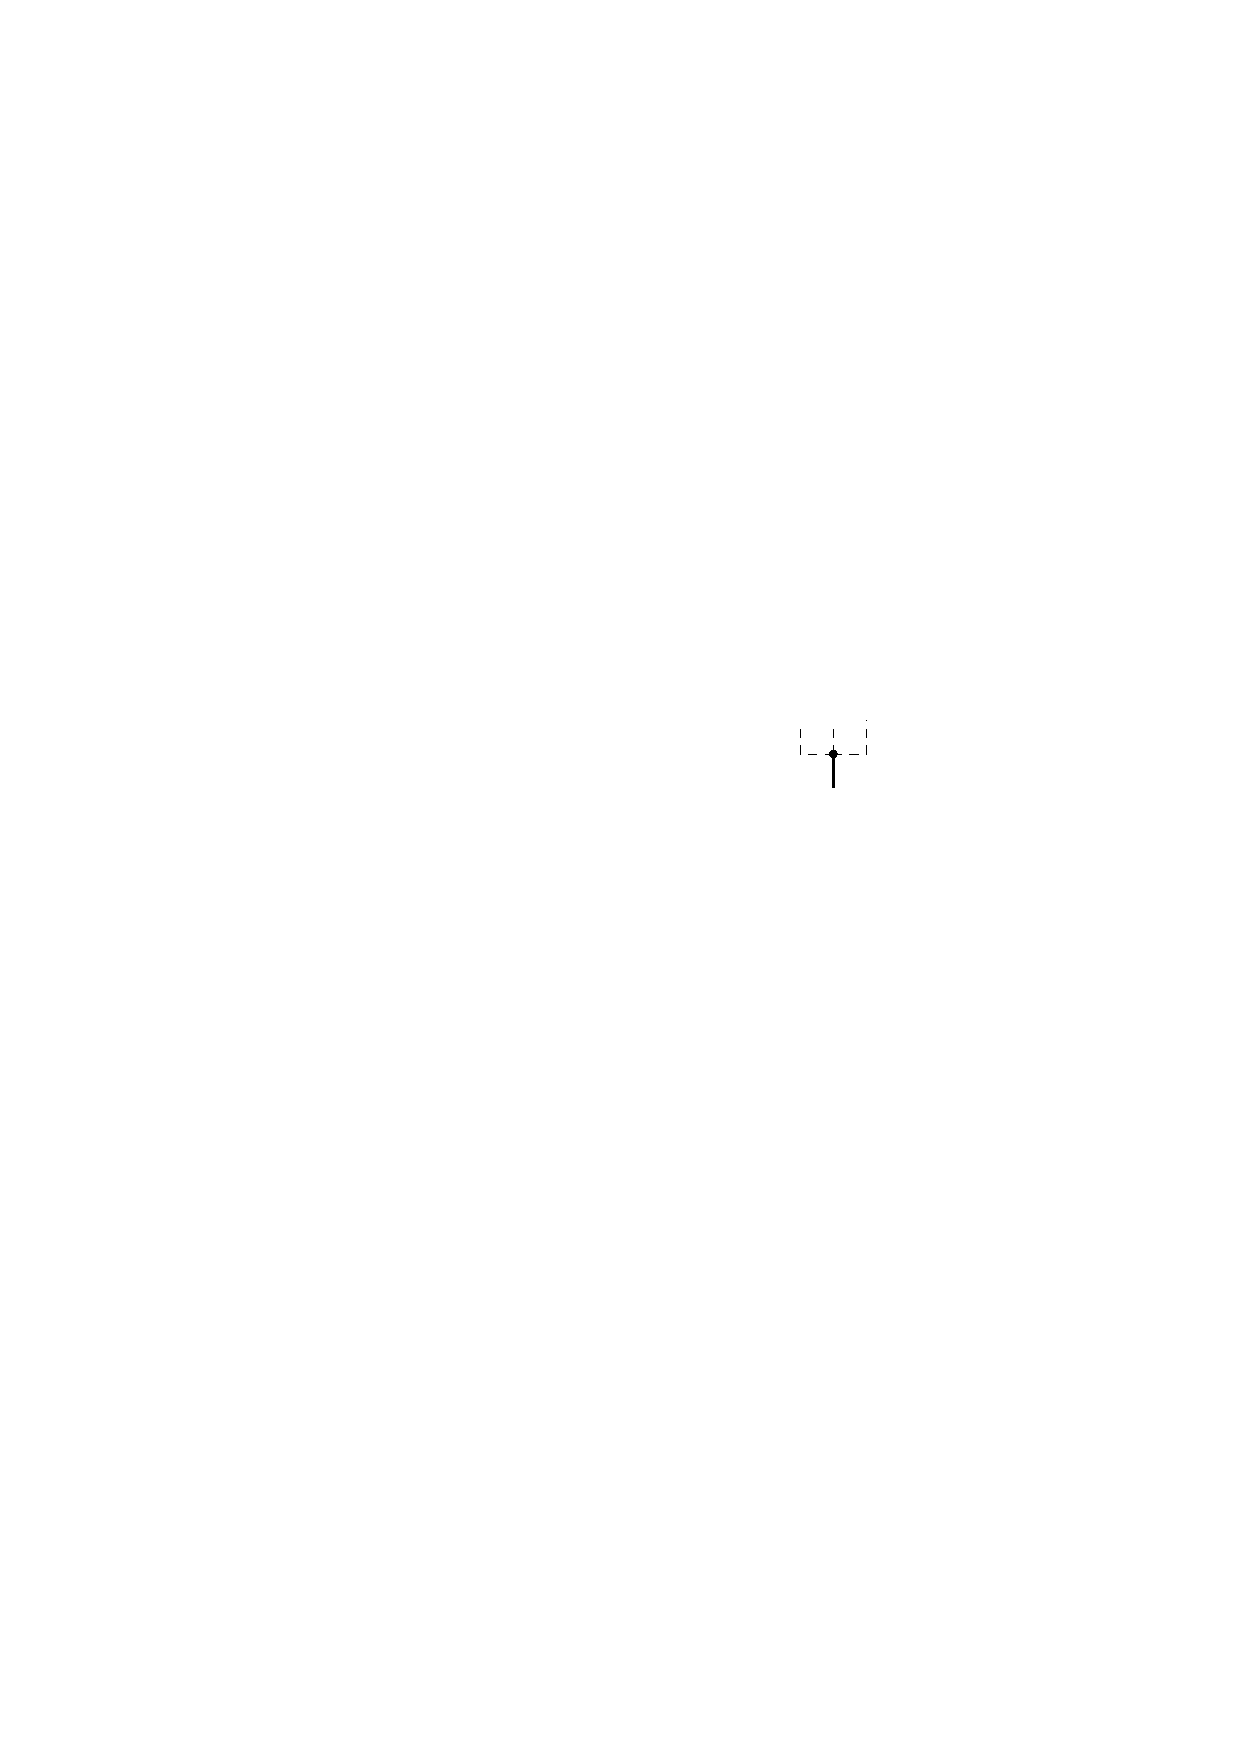
\includegraphics[scale=.8]{oc3_embed/incoming/indeg1}}
        \quad
        \subcaptionbox{2\label{fig:embedindeg2}}
            {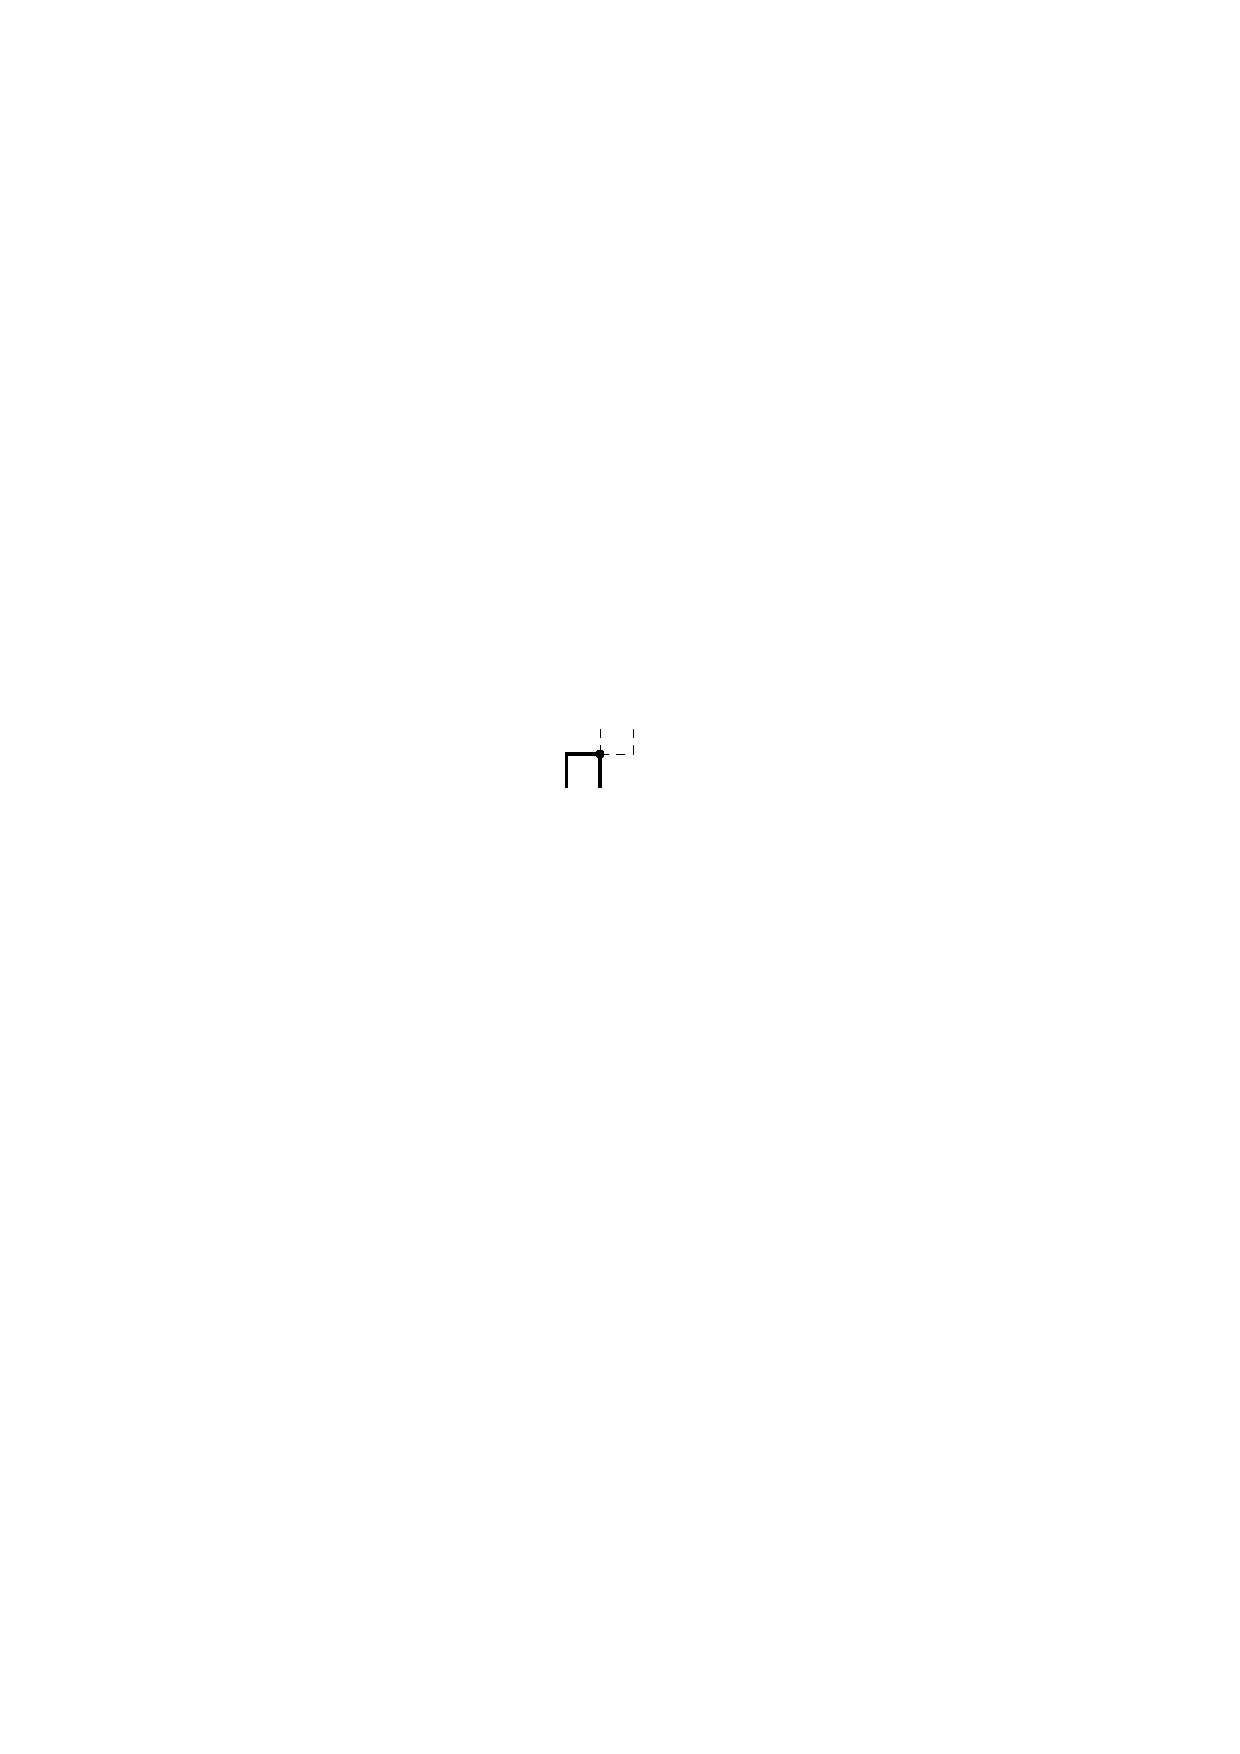
\includegraphics[scale=.8]{oc3_embed/incoming/indeg2}}
        \quad
        \subcaptionbox{3\label{fig:embedindeg3}}
            {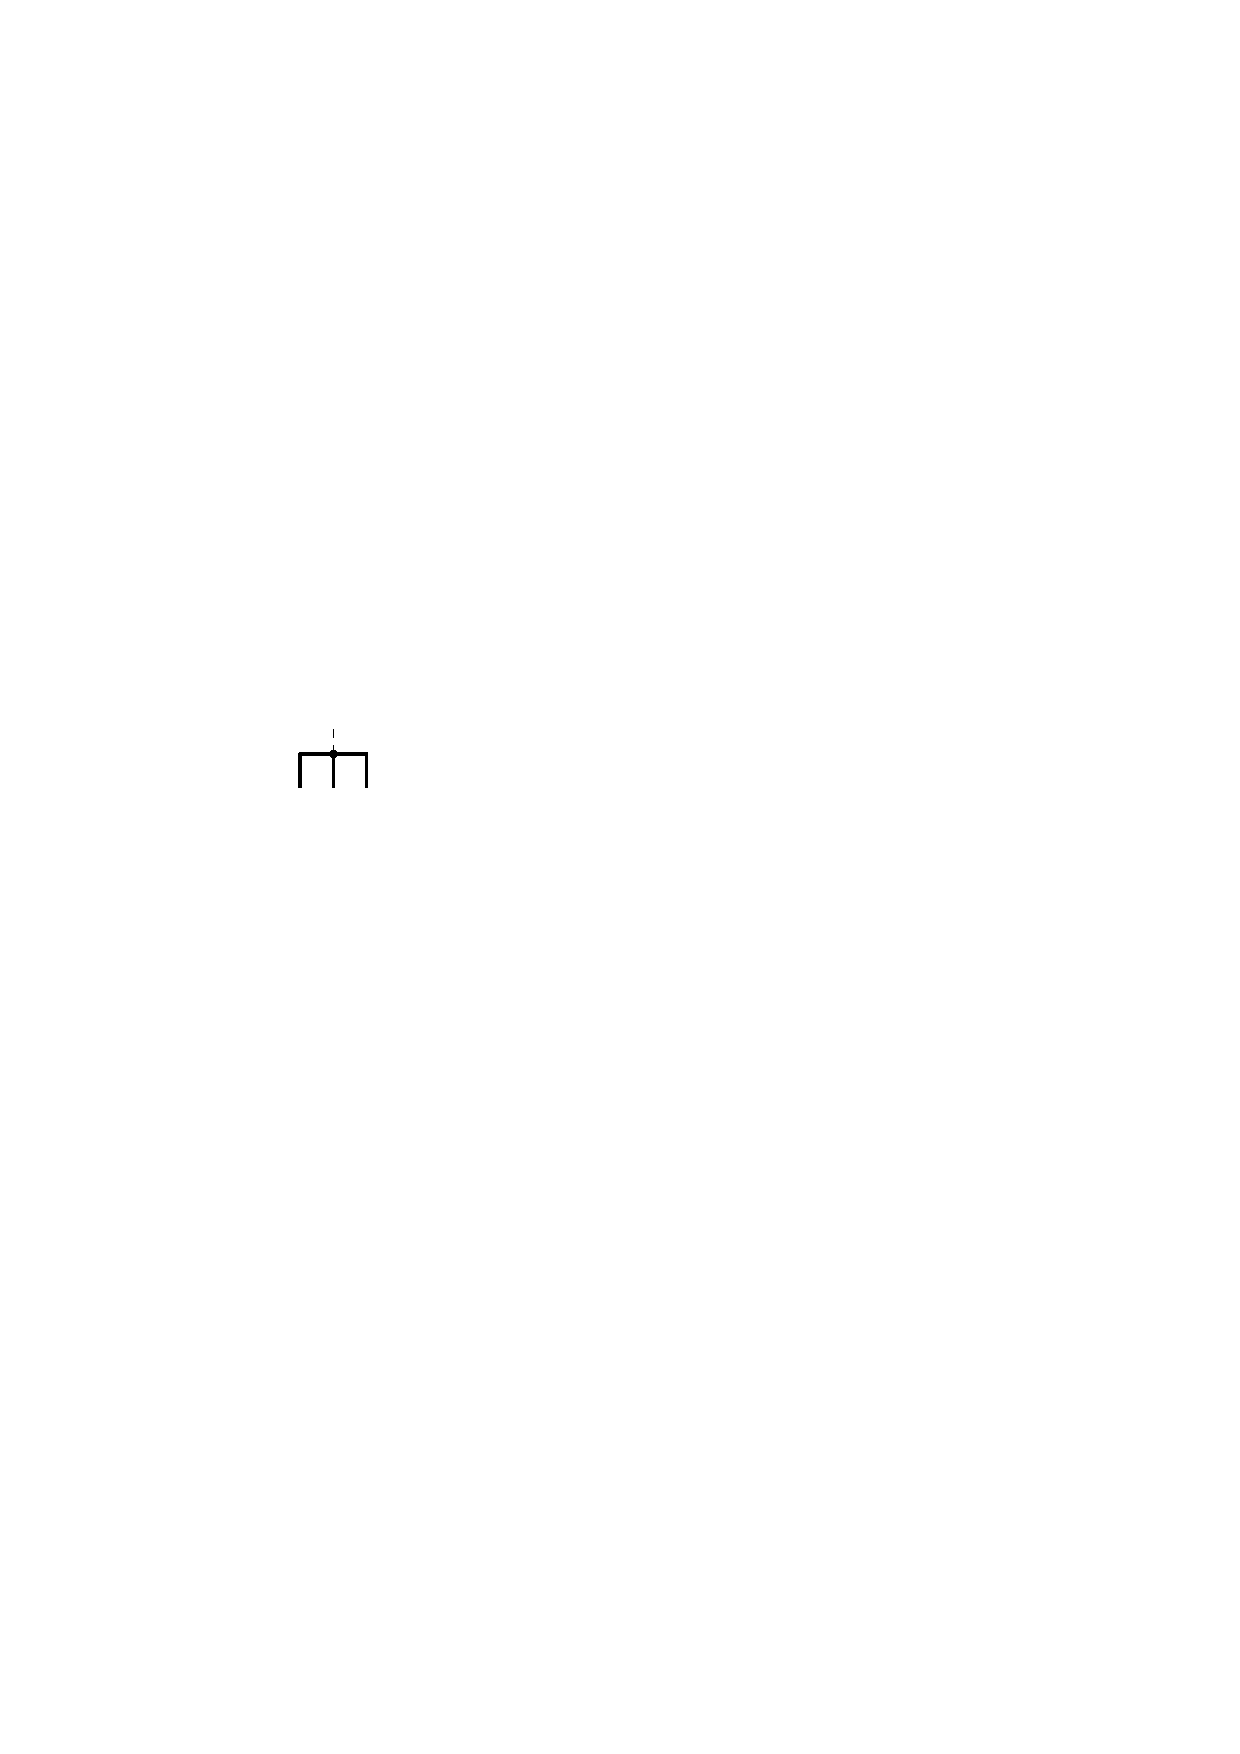
\includegraphics[scale=.8]{oc3_embed/incoming/indeg3}}
        \quad
        \subcaptionbox{4\label{fig:embedindeg4}}
            {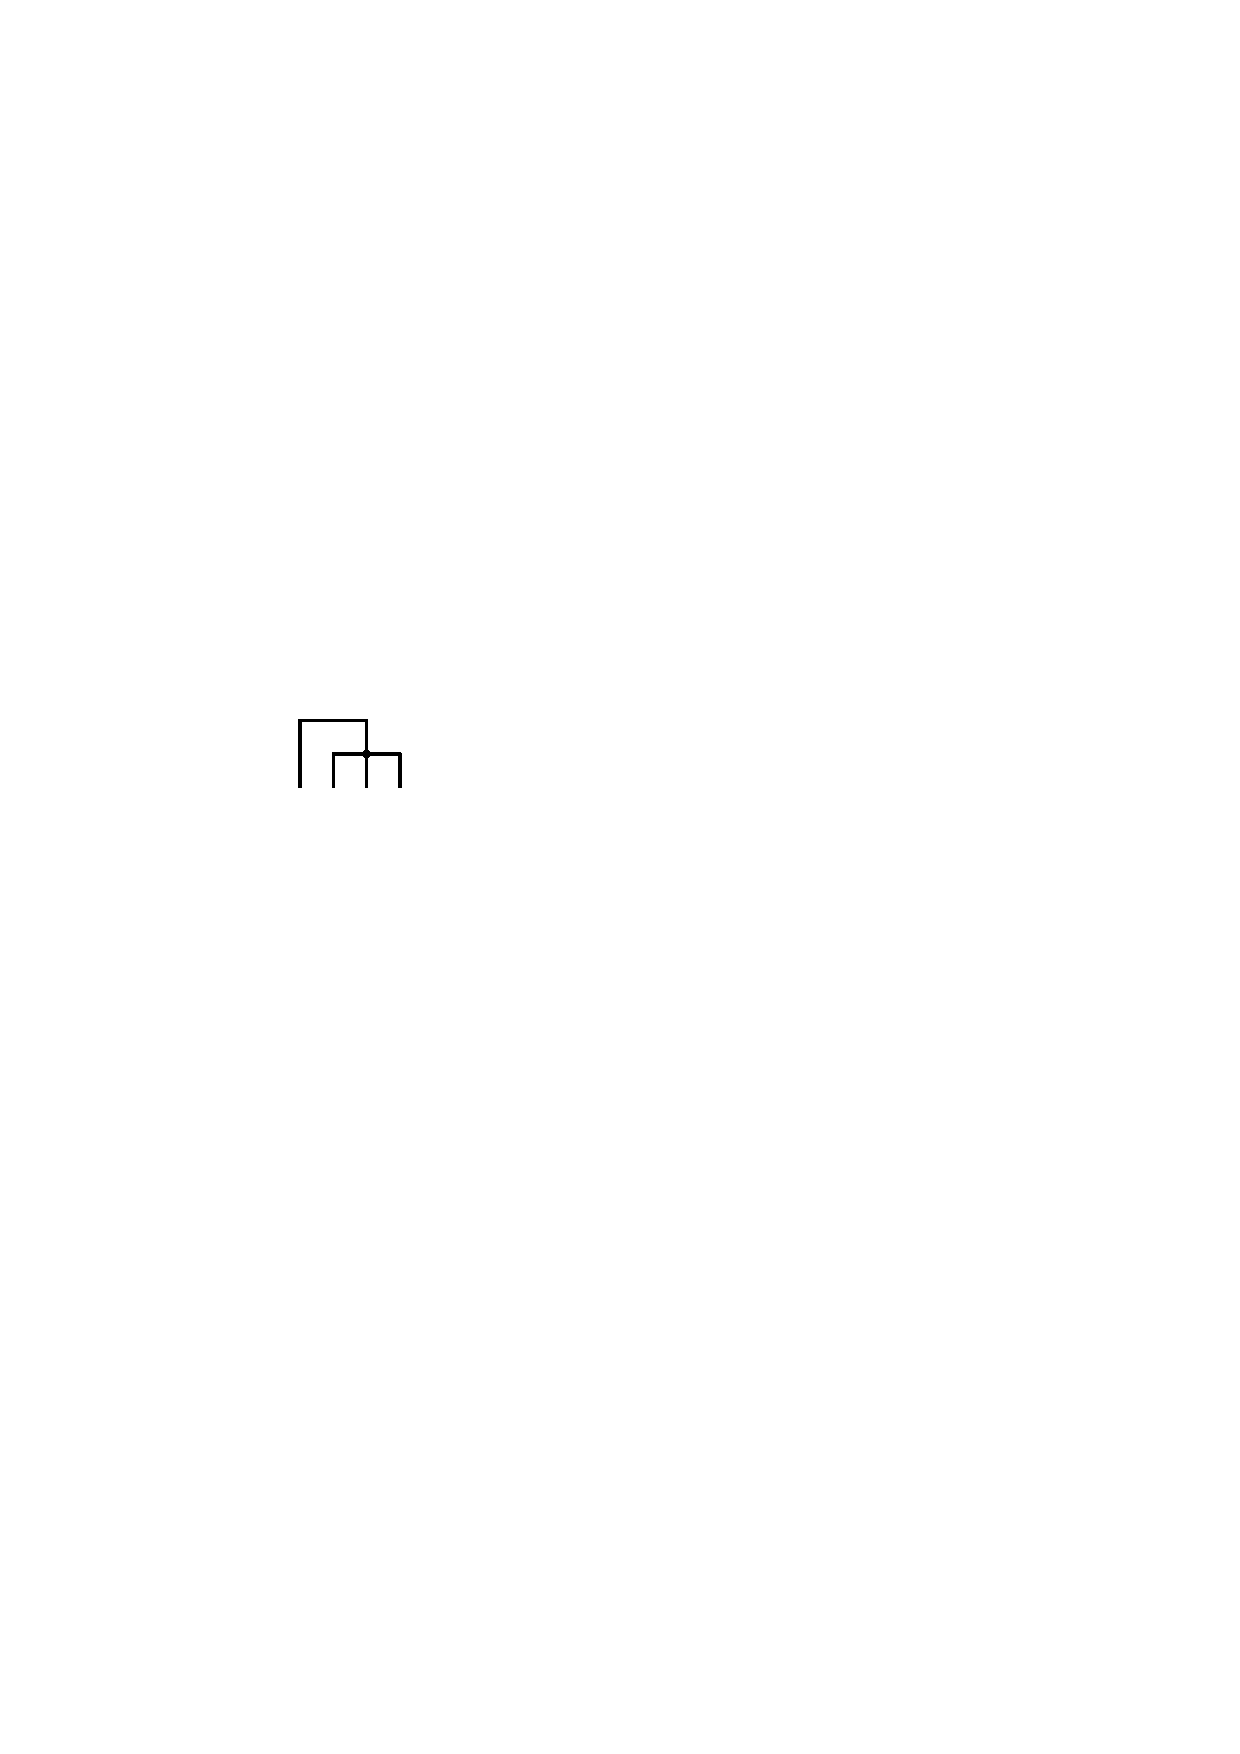
\includegraphics[scale=.8]{oc3_embed/incoming/indeg4}}

        \caption{Die Portzuweisung der bisher offenen, eingehenden Kanten je nach Eingangsgrad. Fett gezeichnet sind die eingehenden Kanten, gestrichelte Kanten sind mögliche Positionen von ausgehenden Kanten.}
        \label{fig:embedin}
\end{figure}

Für die ausgehenden Kanten werden, wie in Abbildung~\ref{fig:embedout} gezeigt, je nach Ausgangsgrad des Knotens folgende Ports zur Verwendung ausgewählt: oben (Ausgangsgrad~1 bis~4), rechts (2--4), links (3, 4), unten (4). Der untere Port wird also nur bei Ausgangsgrad~4 verwendet, was nur bei der Quelle $v_1$ vorkommen kann. Somit befindet sich, außer bei $v_0$, stets eine eingehende Kante am unteren Port. Den Ports werden dann die Kanten nach der Reihenfolge der planaren Einbettung im Uhrzeigersinn, beginnend bei links, dann oben und rechts, zuletzt unten, zugewiesen.

\begin{figure}[h]
        \centering
        \subcaptionbox{0\label{fig:embedoutdeg0}}
            {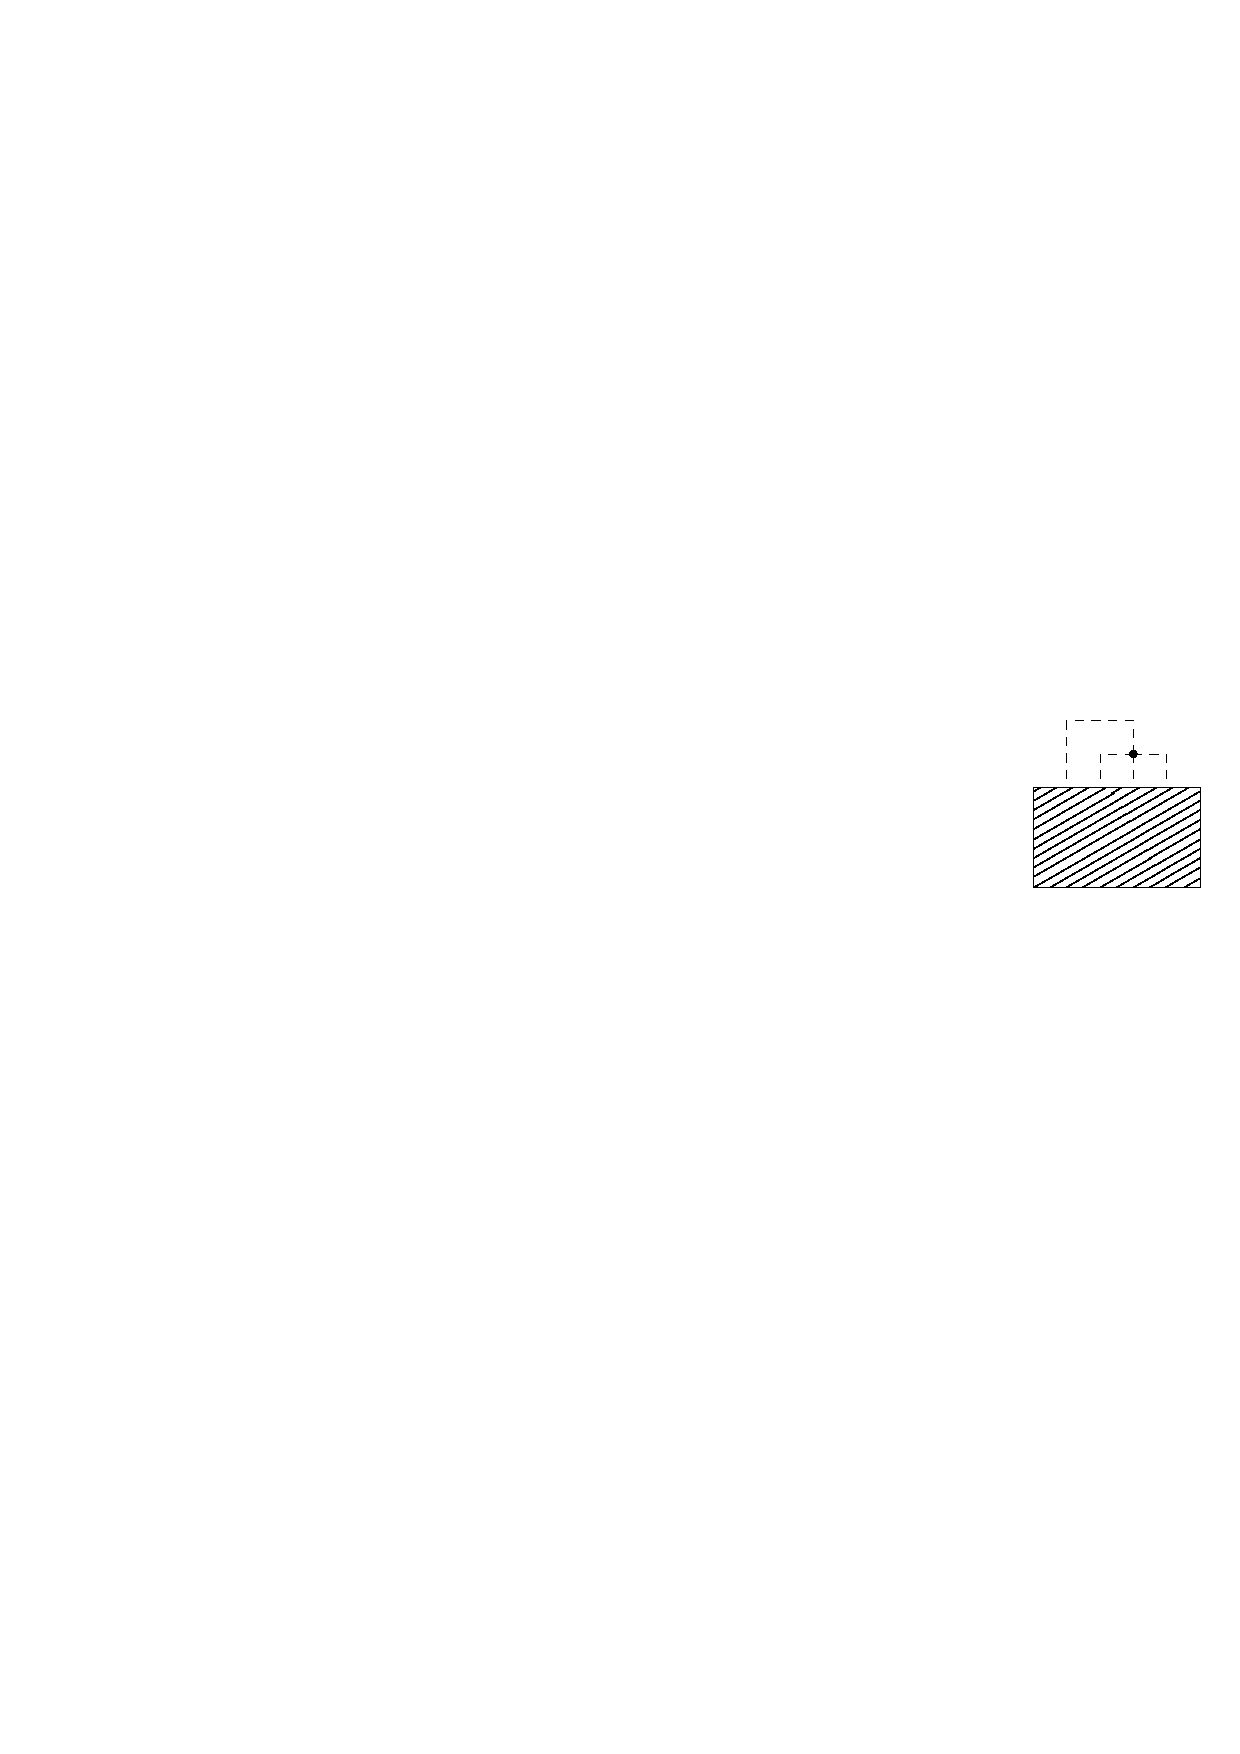
\includegraphics[scale=.8]{oc3_embed/outgoing/outdeg0}}
        \quad
        \subcaptionbox{1\label{fig:embedoutdeg1}}
            {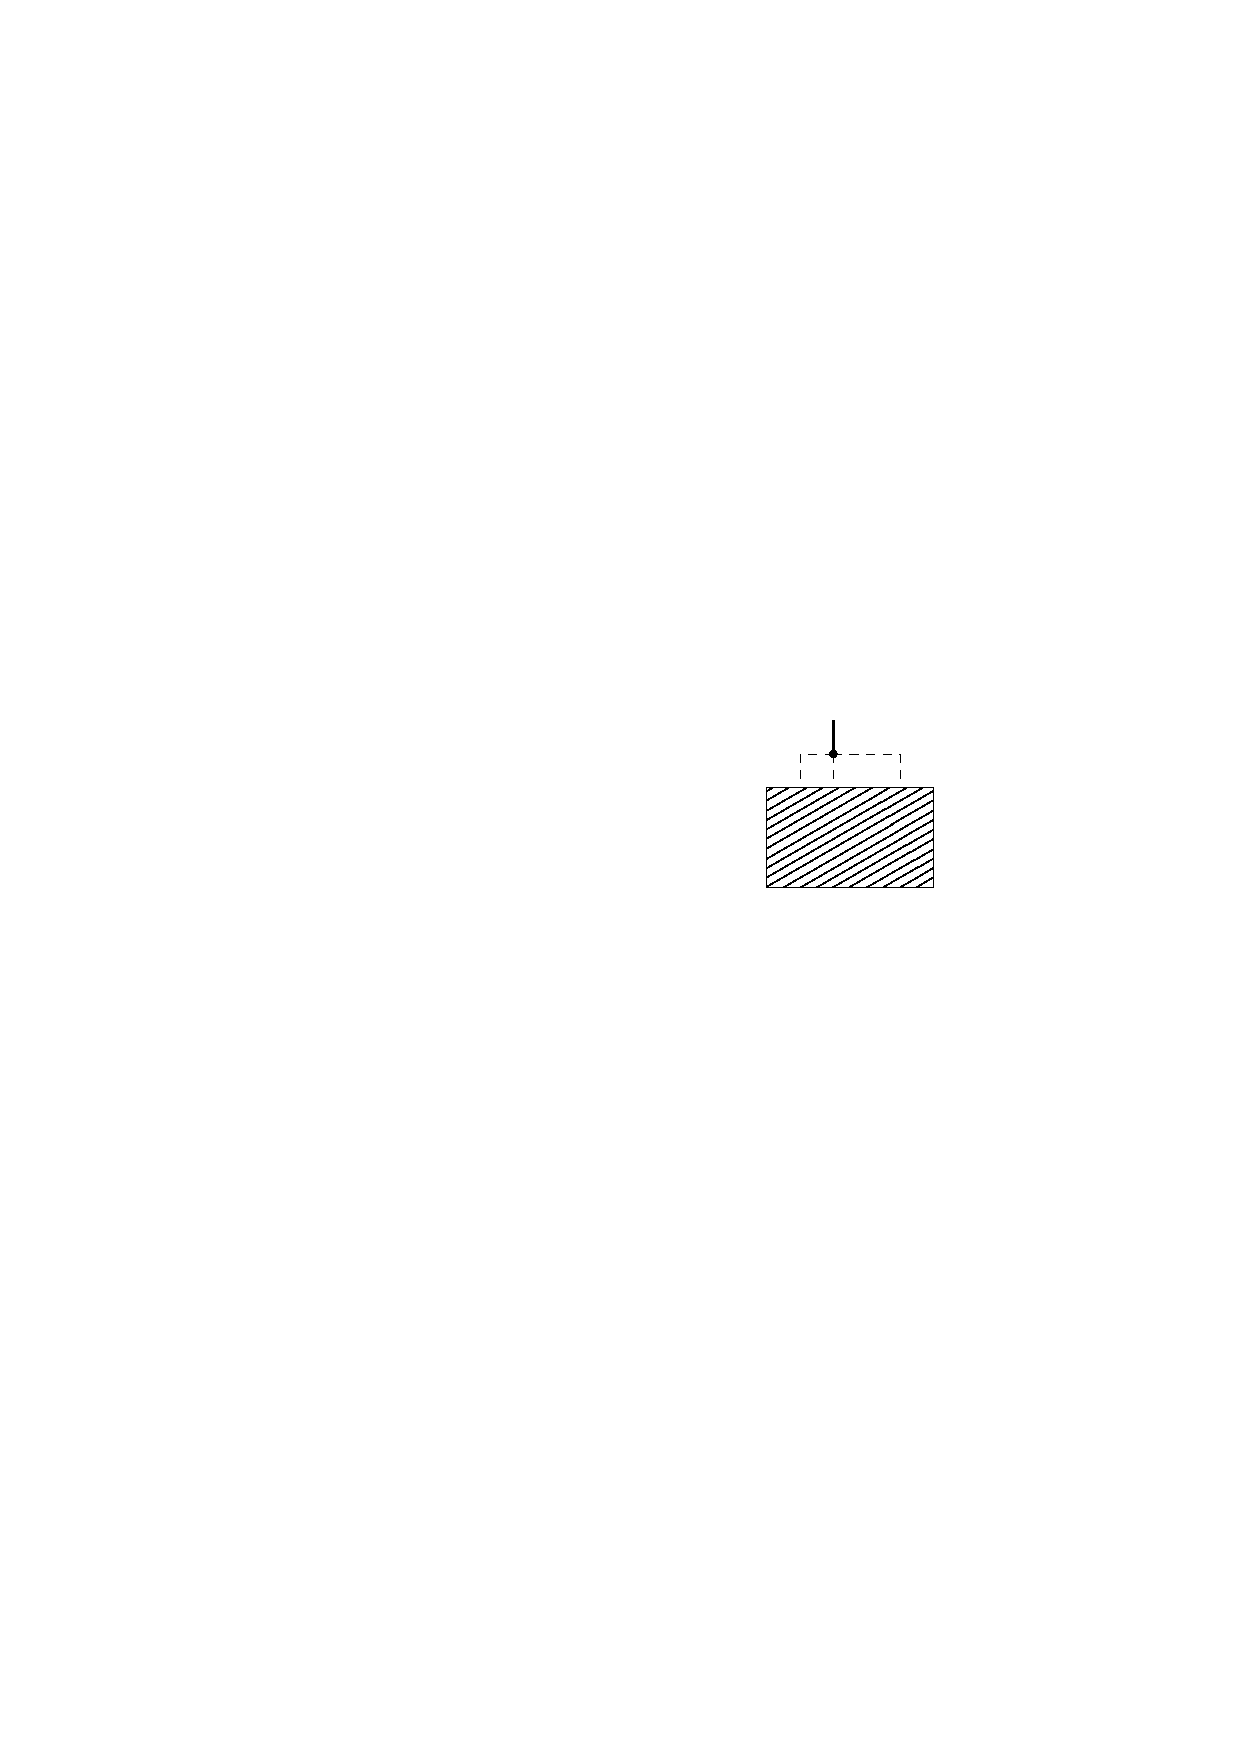
\includegraphics[scale=.8]{oc3_embed/outgoing/outdeg1}}
        \quad
        \subcaptionbox{2\label{fig:embedoutdeg2}}
            {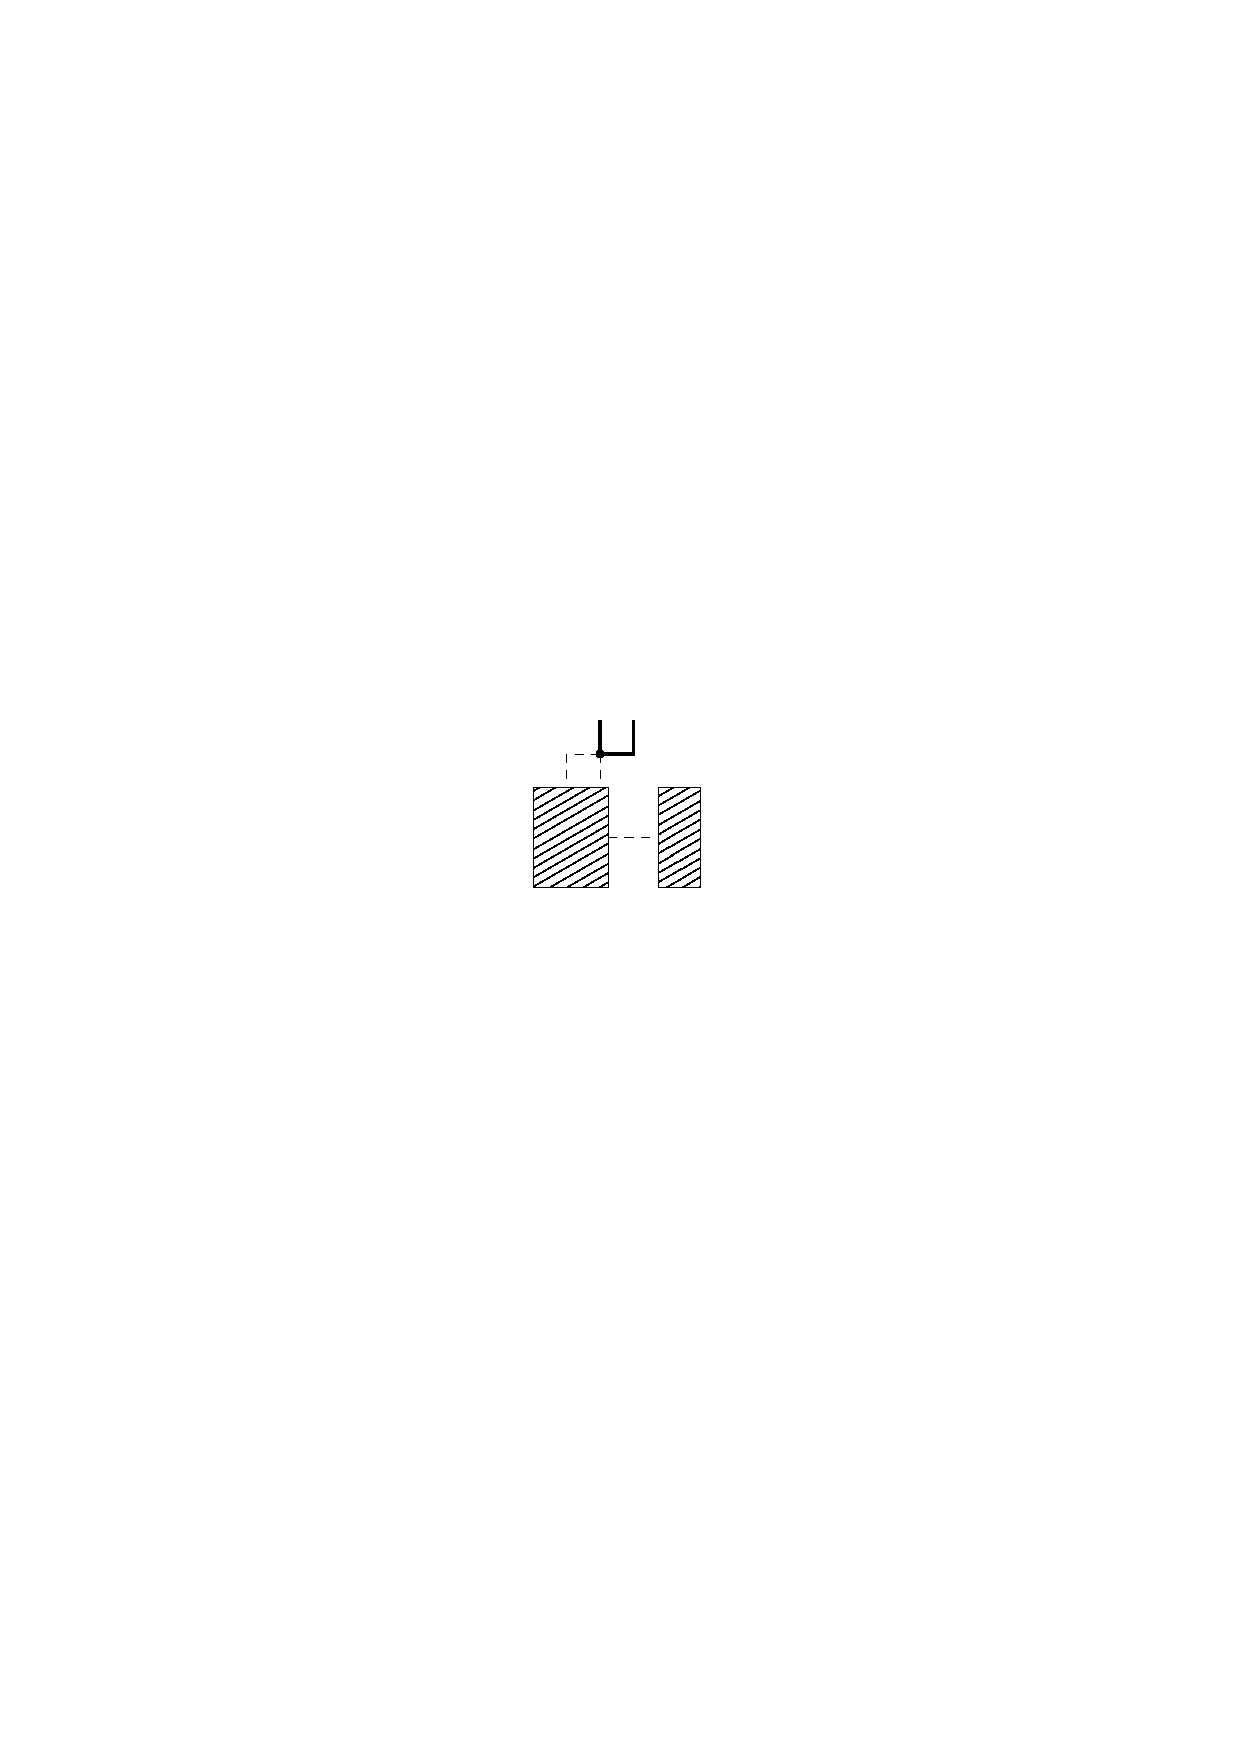
\includegraphics[scale=.8]{oc3_embed/outgoing/outdeg2}}
        \quad
        \subcaptionbox{3\label{fig:embedoutdeg3}}
            {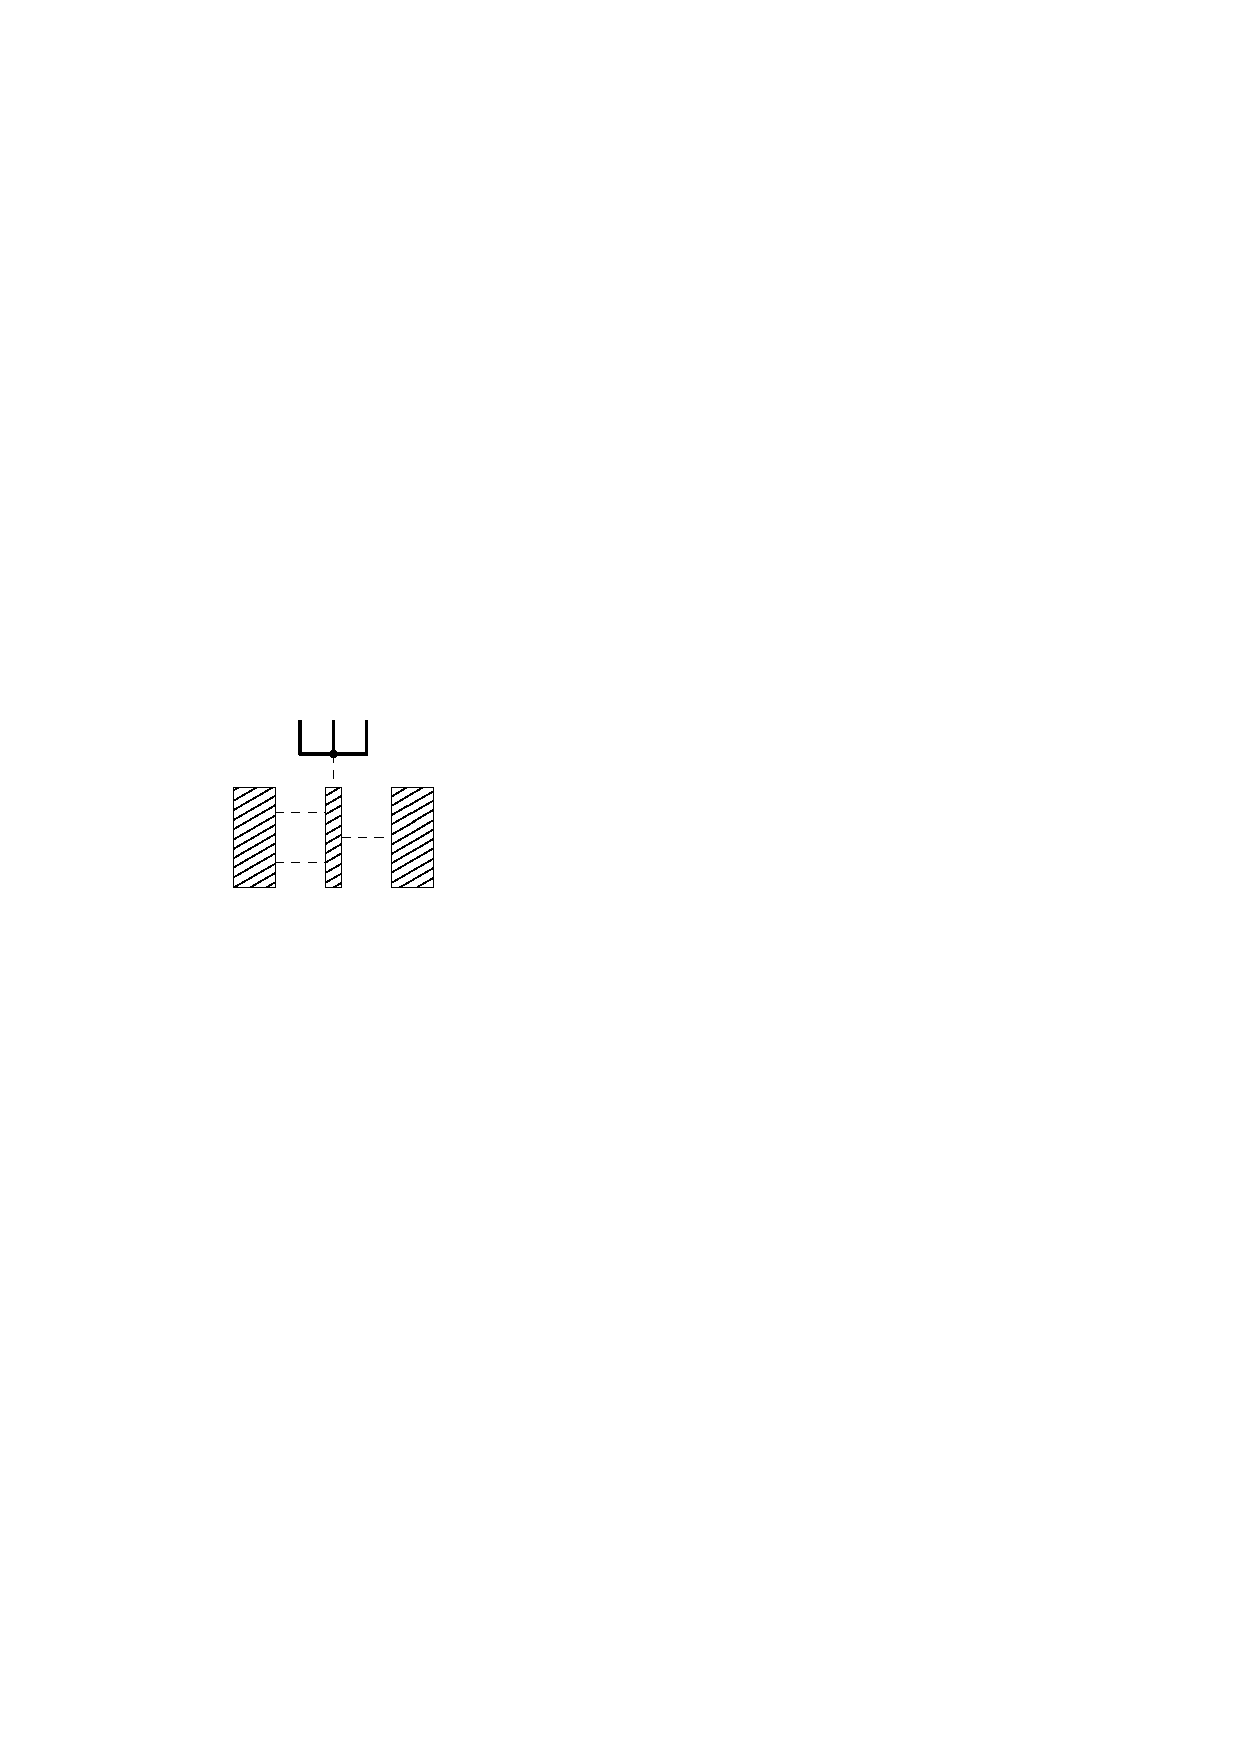
\includegraphics[scale=.8]{oc3_embed/outgoing/outdeg3}}
        \quad
        \subcaptionbox{4\label{fig:embedoutdeg4}}
            {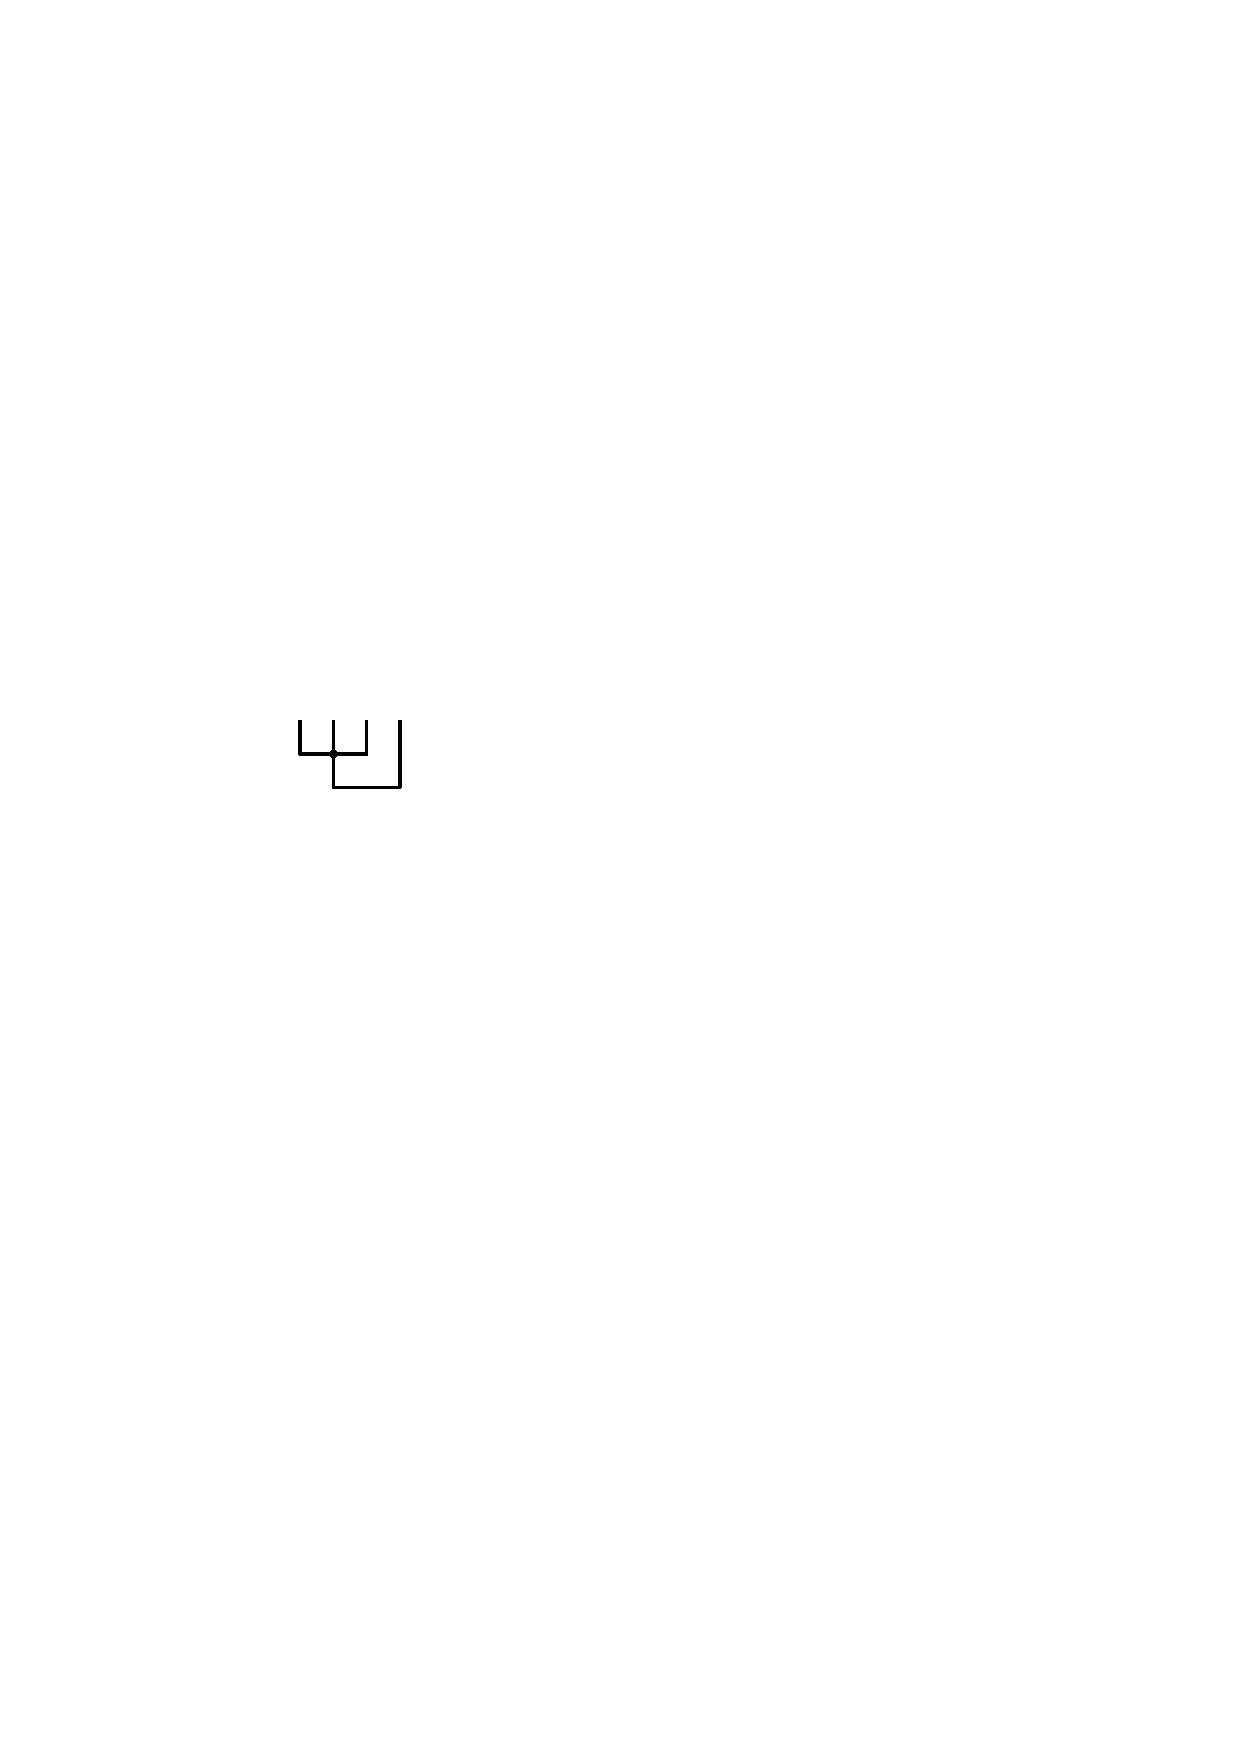
\includegraphics[scale=.8]{oc3_embed/outgoing/outdeg4}}

        \caption{Die Portzuweisung der ausgehenden, neuen offenen Kanten und die neuen Spalten je nach Ausgangsgrad. Fett gezeichnet sind die ausgehenden Kanten, schraffierte Abschnitte stellen bisher gezeichnete Teile des Graphen dar, gestrichelte Kanten sind mögliche Positionen von eingehenden Kanten.}
        \label{fig:embedout}
\end{figure}

Nach diesem Schritt sind die Kanten so den Ports zugewiesen, dass sie mit der planaren Einbettung übereinstimmen.

\subsection{Platzierung der offenen Kanten}

Wenn die Ports den Kanten an einem Knoten zugewiesen wurden und der Knoten in einer Spalte platziert wurde, müssen noch die offenen, ausgehenden Kanten in eine Spalte platziert werden. Die Kante am oberen Port wird in die Spalte des Knotens platziert. Gibt es eine ausgehende Kante am rechten Port, wie in der Zeichnungen aus Abbildung~\ref{fig:embedoutdeg2}, so wird eine neue Spalte rechts des Knotens eingefügt und die Kante in diese Spalte platziert. Wie in der Abbildung zu erkennen, wird dabei der bereits platzierte Teil des Graphen auseinandergezogen. Analog wird eine ausgehende Kante am linken Port in eine neue Spalte links des Knotens platziert, zu sehen in den Abbildung~\ref{fig:embedoutdeg3}. Gibt es eine ausgehende Kante am unteren Port, wie in Abbildung~\ref{fig:embedoutdeg4}, so gibt es auch eine Kante am rechten Port, die bereits in einer neuen Spalte rechts des Knotens platziert wurde. Es wird also noch eine Spalte rechts dieser Spalte hinzugefügt, in die die Kante am unteren Port platziert wird. Nach diesem Schritt sind die neuen offenen Kanten in Spalten platziert.

Für jeden Knoten werden also die Schritte Portzuweisung, Platzierung des Knotens und Platzierung der ausgehenden Kanten durchgeführt, bis alle Knoten platziert sind. Zuletzt werden die Spalten von links nach rechts durchnummeriert und den darin platzierten Knoten und Kanten wird diese Nummer als x"~Koordinate zugewiesen.

Die Bedingungen für die maximale Kantenkomplexität werden auch, bis auf maximal zwei Ausnahmen, eingehalten. Wie an den verschiedenen Fällen für das Zeichnen der Kanten zu erkennen ist, wird jeweils nur höchstens ein Knick pro Knoten hinzugefügt, außer es handelt sich um die offene Kante am unteren Port bei Ausgangsgrad~4 oder die eingehende Kante am oberen Port bei Eingangsgrad~4. Diese Fälle können aber jeweils nur einmal in der Zeichnung auftreten, nämlich an $v_1$ und $v_n$. Außerdem können nicht beide Fälle gleichzeitig auftreten, da die Kantenhälften auf gegenüberliegenden Seiten liegen. Diese beiden halben Kanten mit zwei Knicken werden im schlechtesten Fall also jeweils mit einer halben Kante mit einem Knick verbunden und bilden dann eine Kante mit drei Knicken. Somit kann die Zeichnung zwei Kanten mit drei Knicken haben. In allen anderen Fällen hat die offenen Kante bereits maximal einen Knick und wird dann mit maximal einem weiteren Knick mit dem Zielknoten verbunden, und es ergibt sich eine maximale Komplexität von 2. Obwohl Kanten mit drei Knicken und damit Komplexität~4 auftreten können, nennen wir das Layout OC$_3$, da dies unabhängig von der Kontenzahl jeweils nur konstant viele (zwei) Kanten sind. Damit ist das OC$_3$-Layout fertig und kann zur nächsten Iteration weitergegeben werden, wo die stufenförmigen Kanten entfernt werden.


\section{Eliminierung stufenförmiger Kanten}
\label{sec:sEdgeRemoveAlgo}

Das im letzten Schritt erstellte OC$_3$-Layout ist nicht sehr kompakt, da jeder Knoten in einer eigenen Zeile platziert ist. Außerdem sollen stufenförmige Kanten entfernt werden: Sie stellen ein Problem bei der Konvertierung in ein SC$_2$-Layout dar. Günstigerweise beschreiben Liu et al.~\cite{liu+etal-98} eine Erweiterung, die genau diese Probleme löst. Man vergleiche hierzu die beiden Zeichnungen in Abbildung~\ref{fig:exampleAorthogonal}, wo eine stufenförmige Kante entfernt wird, und die Zeichnungen in Abbildung~\ref{fig:orthognalCompress}, in der keine stufenförmigen Kanten entfernt werden, aber das orthogonale Layout komprimiert wird.

% this is grafo3223
\begin{figure}[h]
        \centering
       \subcaptionbox{Das orthogonale Layout ohne Komprimierung ist $|V|-1 = 38$ Gittereinheiten hoch.\label{fig:smoothOknessRaw} }[0.3\textwidth]
            {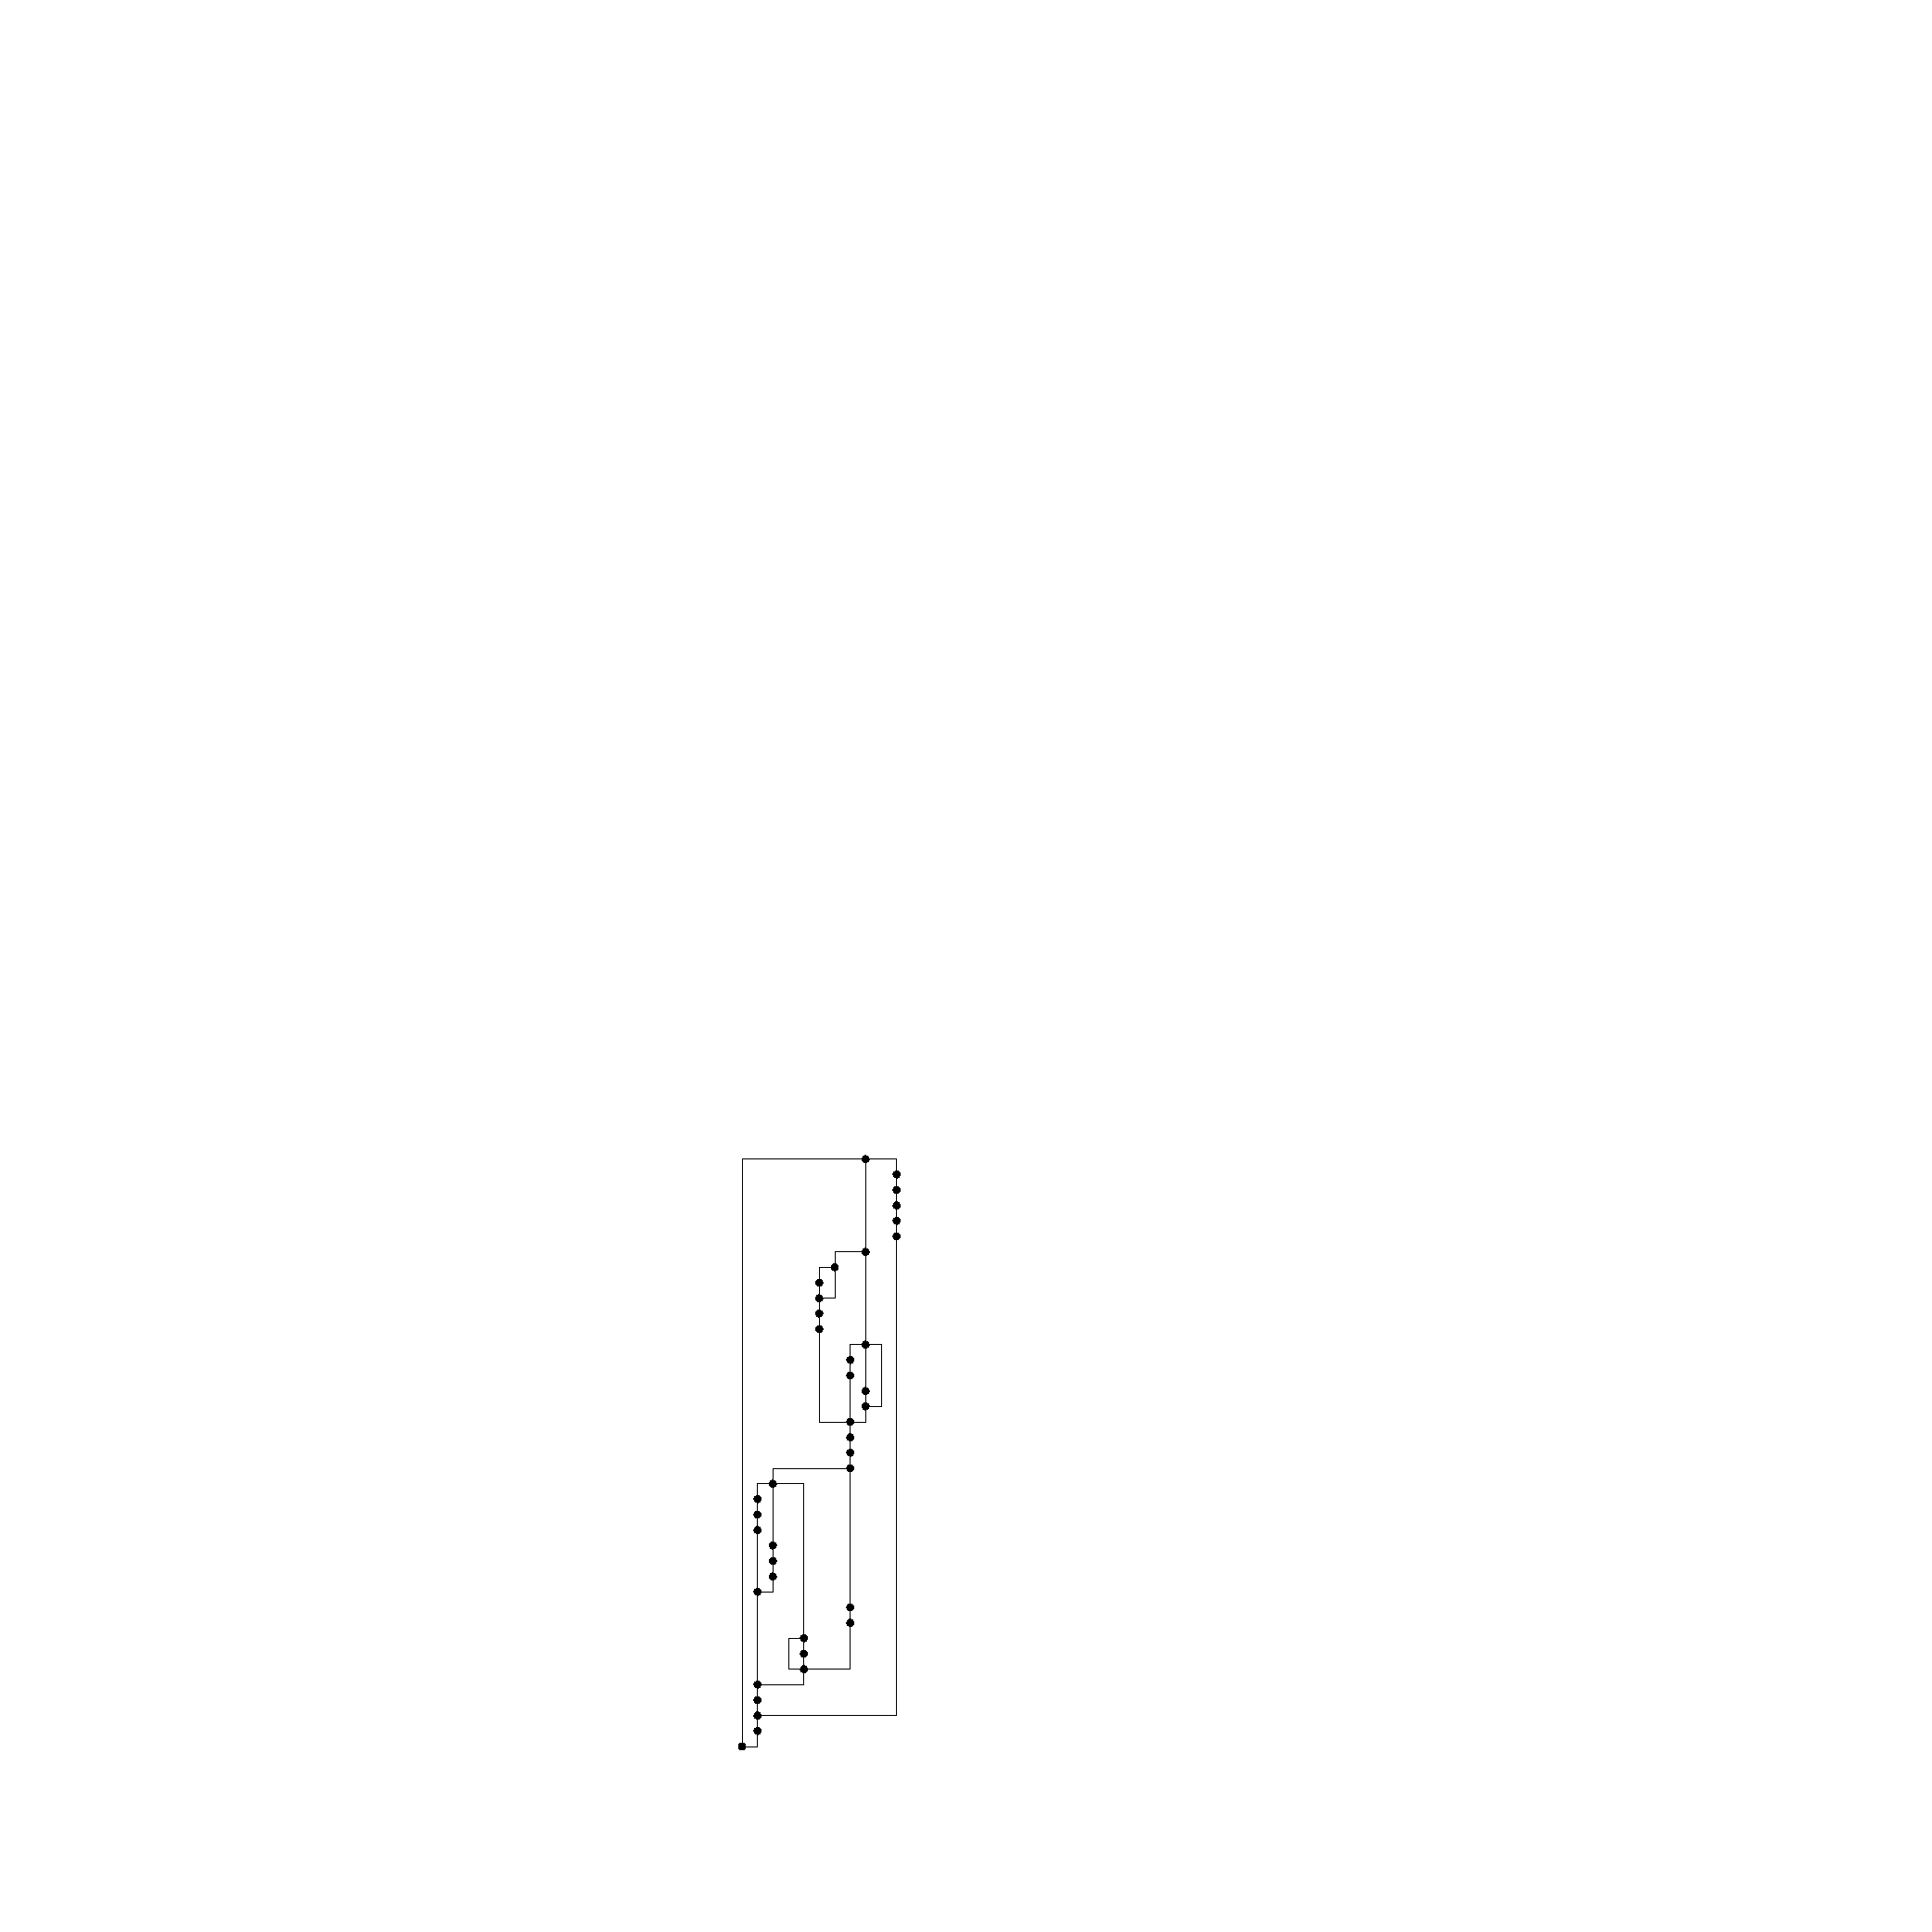
\includegraphics[scale=.7]{compressableGraph/isUncompressed}}
        \quad
       \subcaptionbox{Nach Komprimierung bleiben 20 Gittereinheiten Höhe.\label{fig:smoothOknessCompressed} }[0.3\textwidth]
            {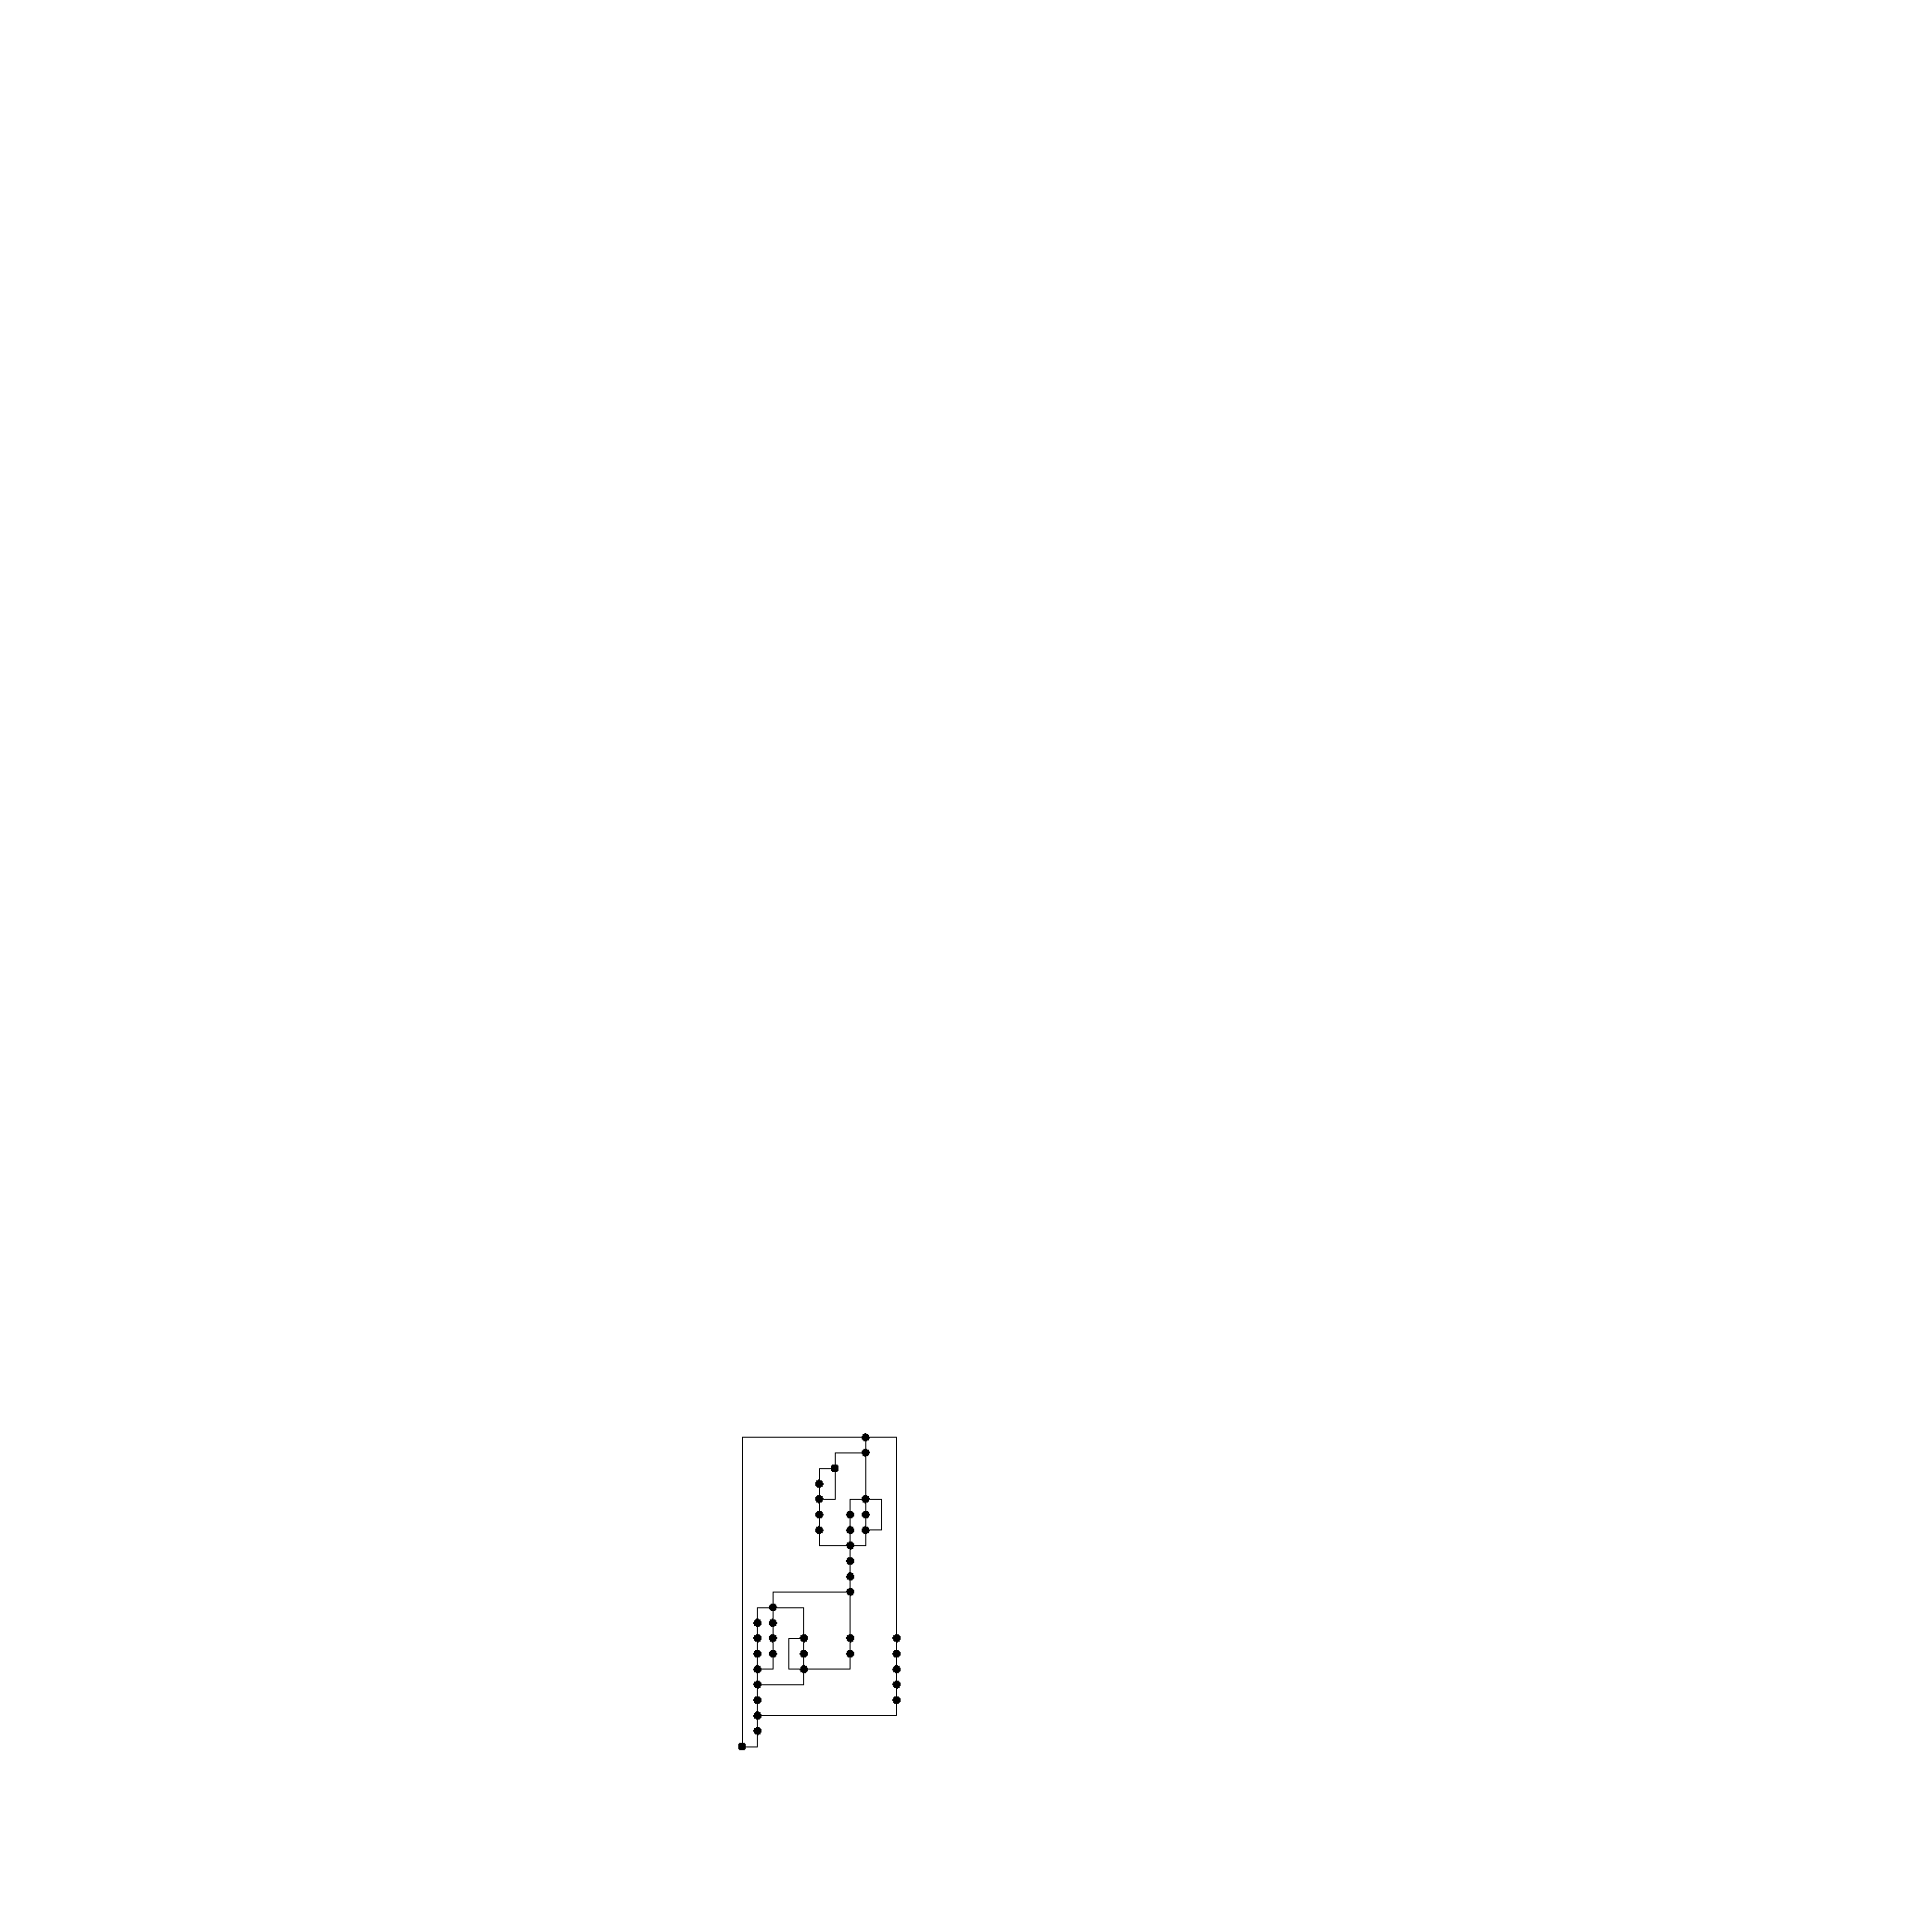
\includegraphics[scale=.7]{compressableGraph/isCompressed}}
        \quad
       \subcaptionbox{Auch die glatt"=orthogonale Zeichnung ist nur 10 Gittereinheiten breit.\label{fig:smoothOknessSmooth} }[0.3\textwidth]
            {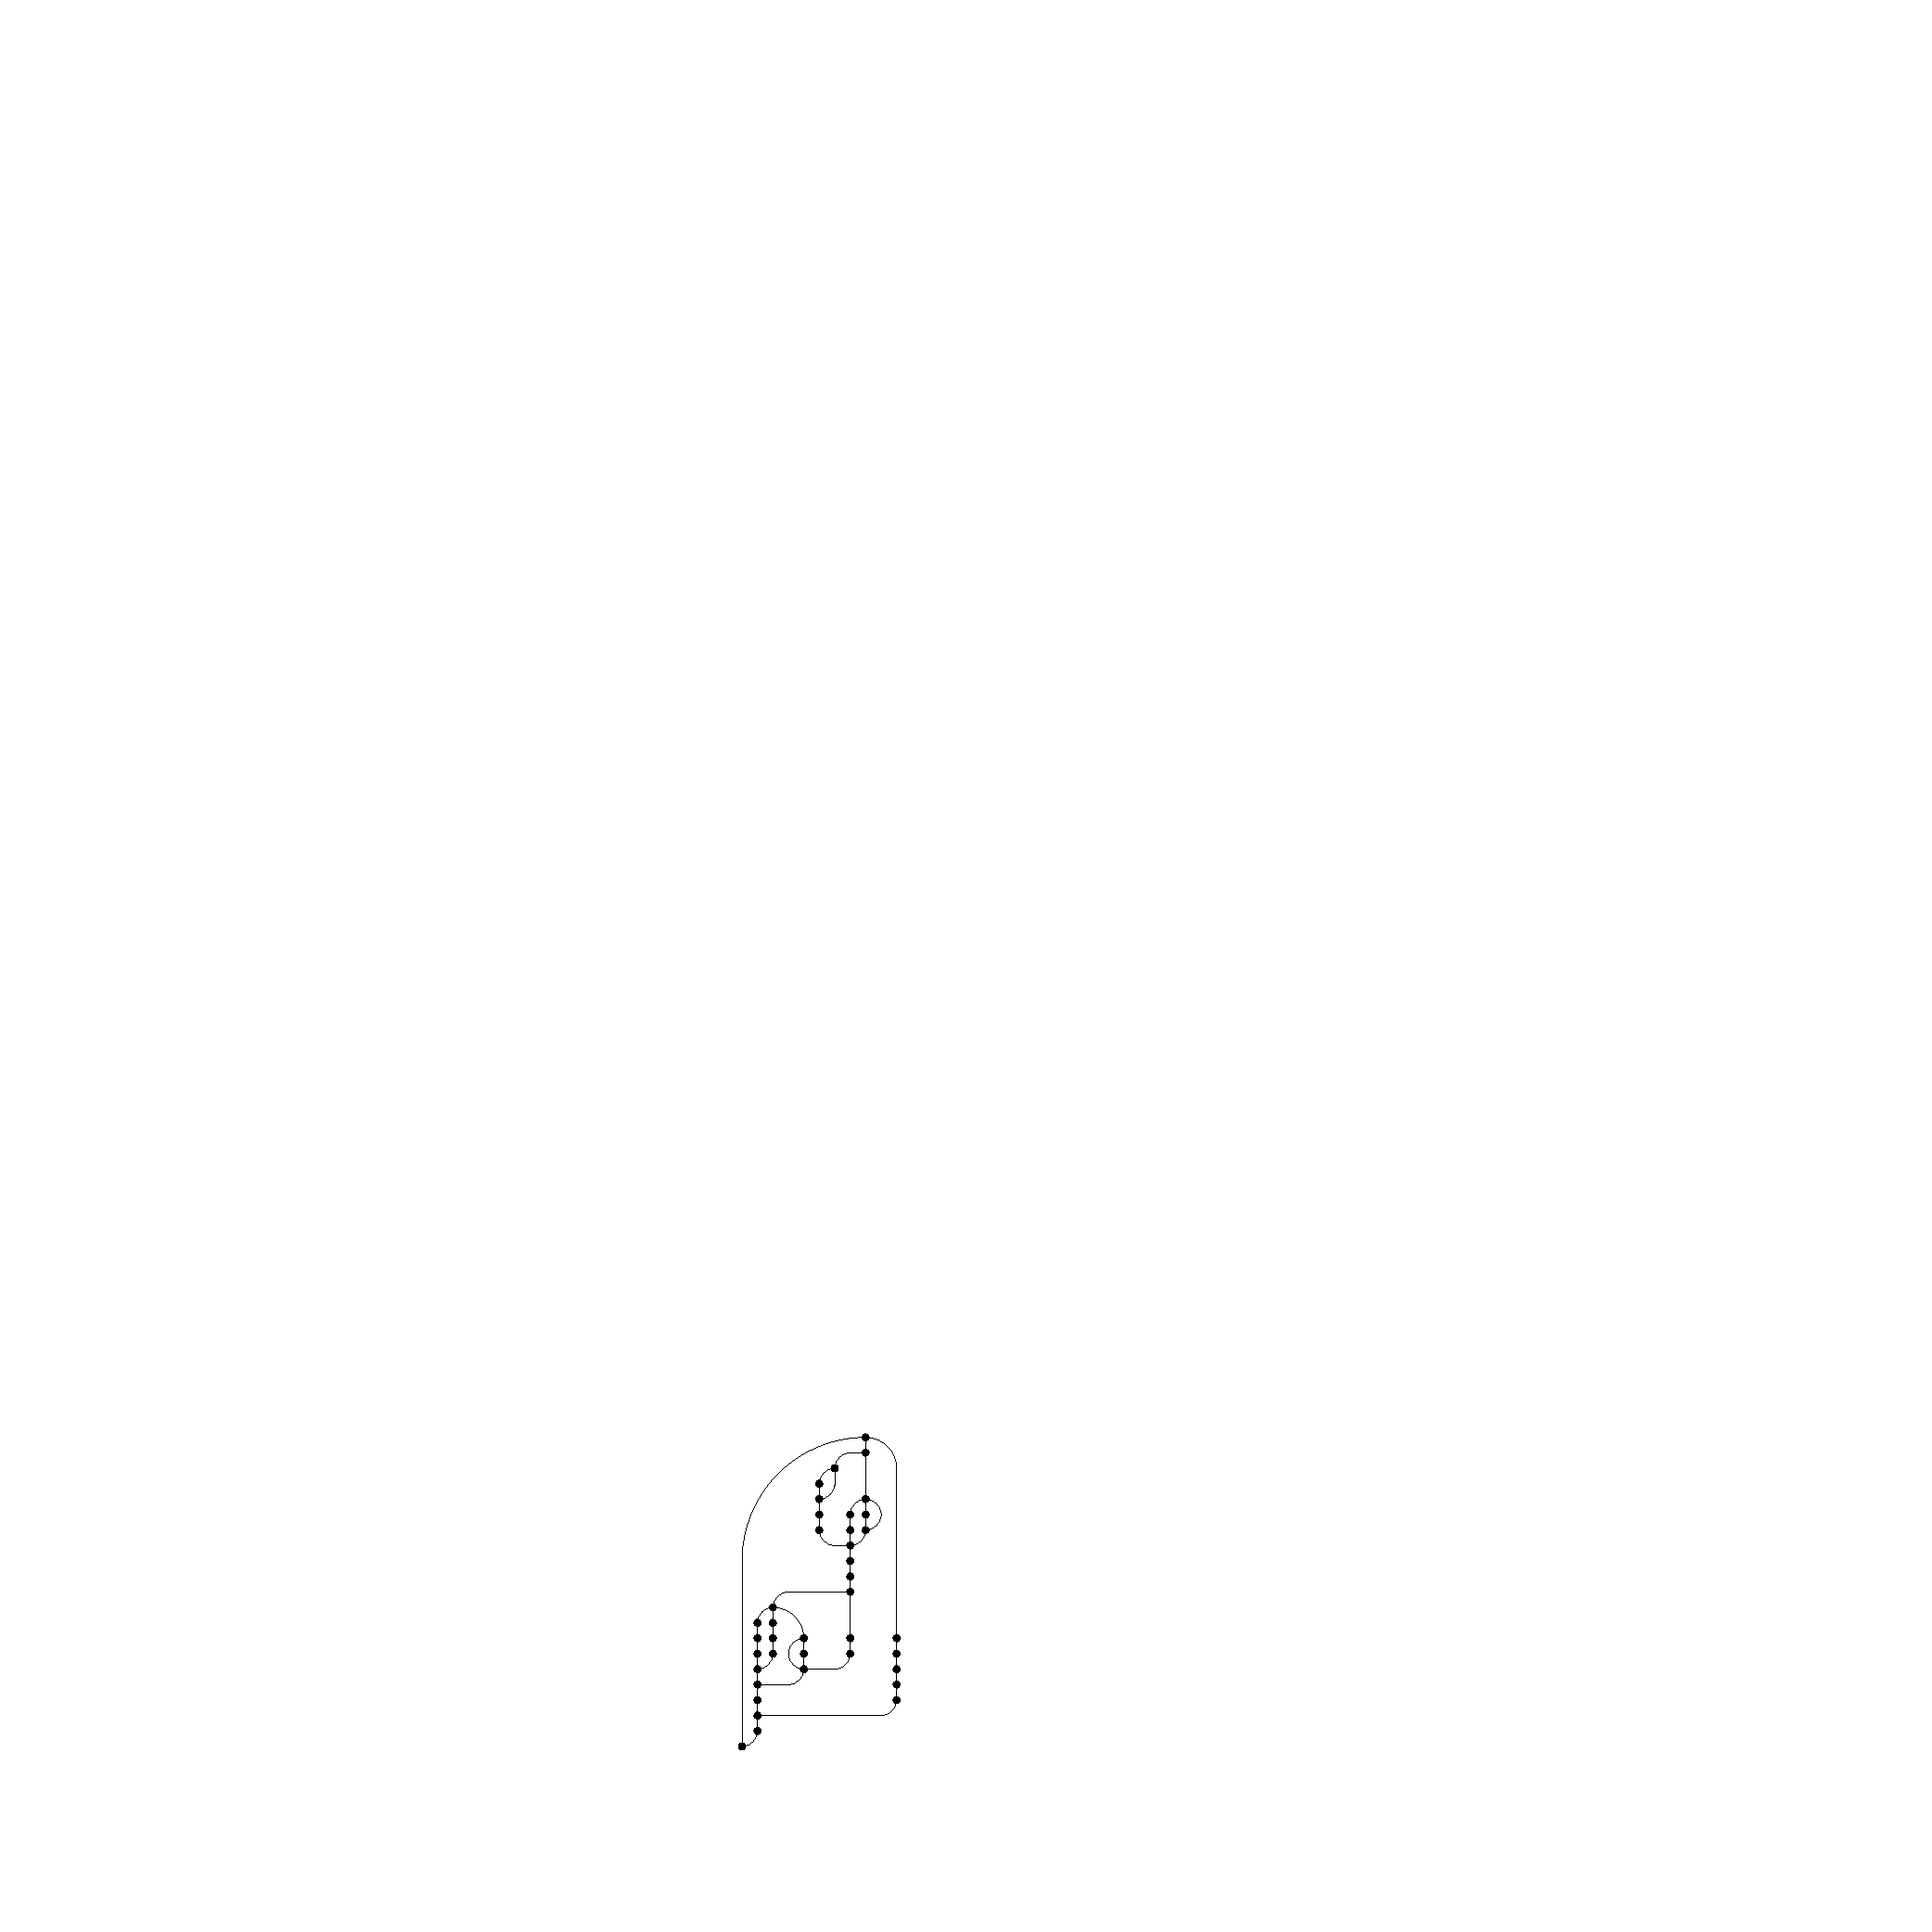
\includegraphics[scale=.7]{compressableGraph/isSmooth}}
 
 
        \caption{Ein Graph mit 39 Knoten, der zwar keine stufenförmigen Kanten enthält, aber dessen Höhe dennoch im Kompressionsschritt beinahe halbiert wird. Die drei Zeichnungen sind hier mit der selben Gittergröße abgebildet und geben somit die Größenverhältnisse korrekt wieder.}
        \label{fig:orthognalCompress}
\end{figure}

\emph{Stufenförmige Kanten} (englisch \emph{zig-zags}) bestehen aus zwei horizontalen Liniensegmenten, die mit einem vertikalen Liniensegment verbunden sind. Eine Kante $(v_i, v_k)$, mit $i < k$ gemäß der $st$-Ordnung, ist stufenförmig, wenn die Kante am rechten Port von $v_i$ und am linken Port von $v_k$ ist. In Abbildung~\ref{fig:exampleAorthogonalNocompress} ist die Kante $(1,2)$ eine solche stufenförmige Kante. Zwei so verbundene Knoten werden in einer Menge von Knoten, einem \emph{Plateau} zusammengefasst. Sind mit diesen Knoten weitere Knoten durch stufenförmige Kanten verbunden, werden diese ebenfalls im selben Plateau zusammengefasst. Somit sind zuletzt alle Knoten in einer "`Treppe"' in einem Plateau.

Diese Plateaus werden nun als Knoten eines neuen orientierten Graphen verwendet. Zwischen zwei verschiedenen Plateaus $P_1, P_2$ fügen wir eine Kante ein, falls es im Originalgraphen eine Kante $(v_i, v_k)$ mit $v_i \in P_1$ und $v_k \in V_2$ gibt. Bei Liu et al.~\cite{liu+etal-98} findet sich ein Beweis, dass auf diese Weise die Kanten zwischen zwei Plateaus eindeutig orientiert sind und jeder Knoten zu genau einem Plateau gehört. 

Im Beispielgraphen $G_\text{E}$ und der Zeichnung aus Abbildung~\ref{fig:exampleAorthogonalNocompress} sähen die Plateaus $V_\text{P}$ und ihr Graph $G_\text{P}$ so aus:

\[G_\text{P} = (V_\text{P}, E_\text{P})\]
\[V_\text{P} = \{\{0\}, \{1, 2\}, \{3\}, \{4\}\}\]
\[E_\text{P} = \{(\{0\}, \{1, 2\}), (\{0\}, \{4\}), (\{1, 2\}, \{3\}), (\{1, 2\}, \{4\}), (\{3\}, \{4\})\}\]


Im so entstandenen Graphen erhält das Plateau mit $v_1$ die Höhe~$1$. Dann erhält jedes andere Plateau jeweils die um~1 inkrementierte Höhe seines höchsten Vorgängers, bis alle Plateaus eine Höhe erhalten haben. Zuletzt weisen wir den Knoten die Höhe ihres Plateaus als neue y"~Koordinate zu.

Offensichtlich kann es nun keine stufenförmigen Kanten mehr geben, da die entsprechenden Knoten im gleichen Plateau sind und somit die gleiche y"~Koordinate haben. Alle Knoten eines Plateaus liegen auf einer horizontalen Linie. Die vormals stufenförmigen Kanten bestehen nun aus einem horizontalen Liniensegment.

\section{Konvertierung in ein SC$_2$-Layout}
\label{sec:sc2conversion}

Im letzten Schritt wurde ein OC$_3$-Layout erstellt, das im nächsten Schritt für ein planares SC$_2$-Layout angepasst werden soll. Für den Test der Planarität werden die glatt"=orthogonalen Kanten gezeichnet und auf Überschneidungen geprüft. Dafür ist es nötig, das Aussehen der Kanten zu kennen. In Abschnitt~\ref{sec:smooth_definition} wurde bereits erwähnt, dass eine Kante zwischen zwei Knoten anhand der Positionen der Knoten und der Portzuweisung der Kante an den beiden Knoten bereits eindeutig gezeichnet werden kann. Dabei sollen nur orthogonale Kanten mit maximaler Komplexität~3 betrachtet werden.

Als Ergebnis soll stets eine glatt"=orthogonale Kante mit maximaler Komplexität~2 stehen. Wie dies zu bewerkstelligen ist, wird im folgenden erklärt. Die \emph{Steigung} einer Kante sei der kleinere der beiden Winkel zwischen der Gerade durch die beiden Endpunkte der Kante und der x"~Achse.

\begin{figure}[h]
        \centering
        \subcaptionbox{I"~Kante\label{fig:sc2conversionIEdge}}
            {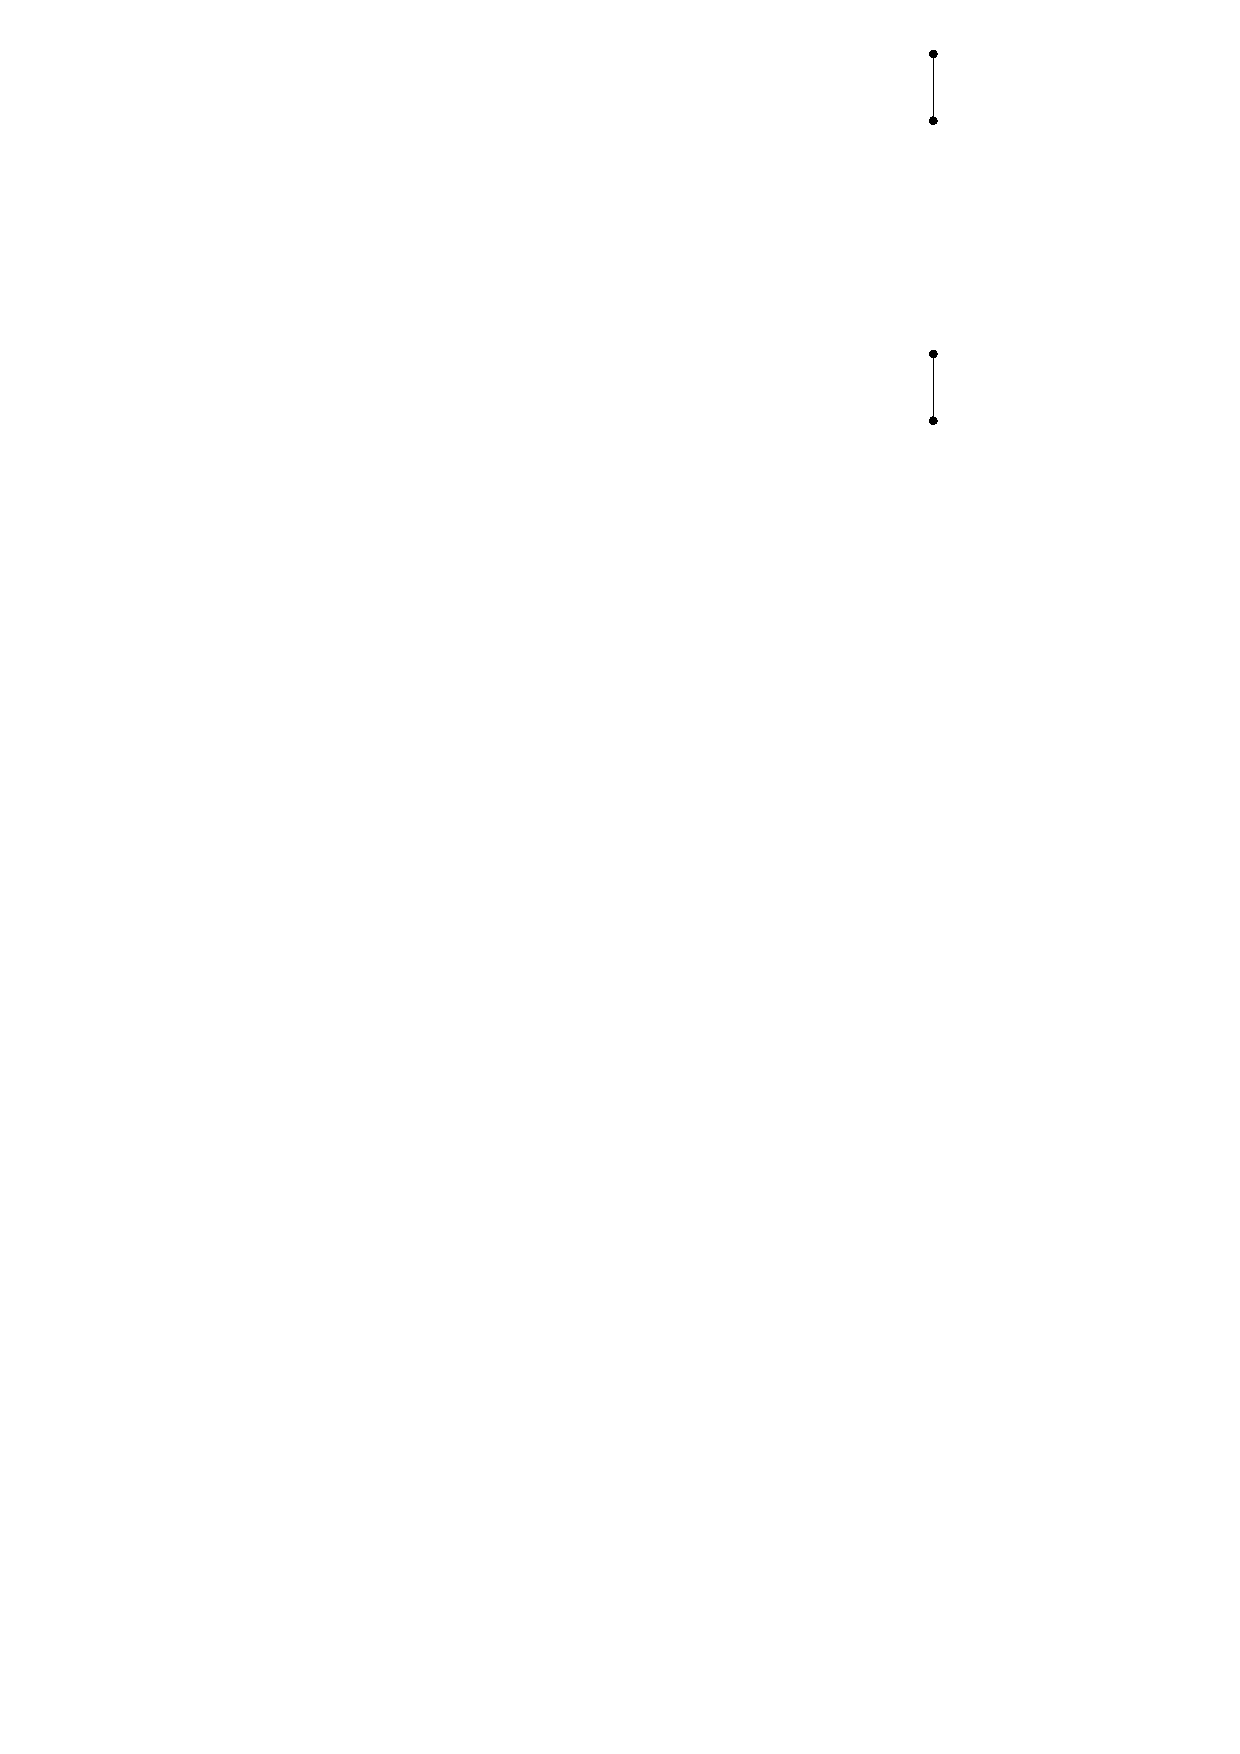
\includegraphics[scale=.8]{sc2_conversion/IEdge}}
        \quad
        \subcaptionbox{L"~Kante\label{fig:sc2conversionLEdge}}
            {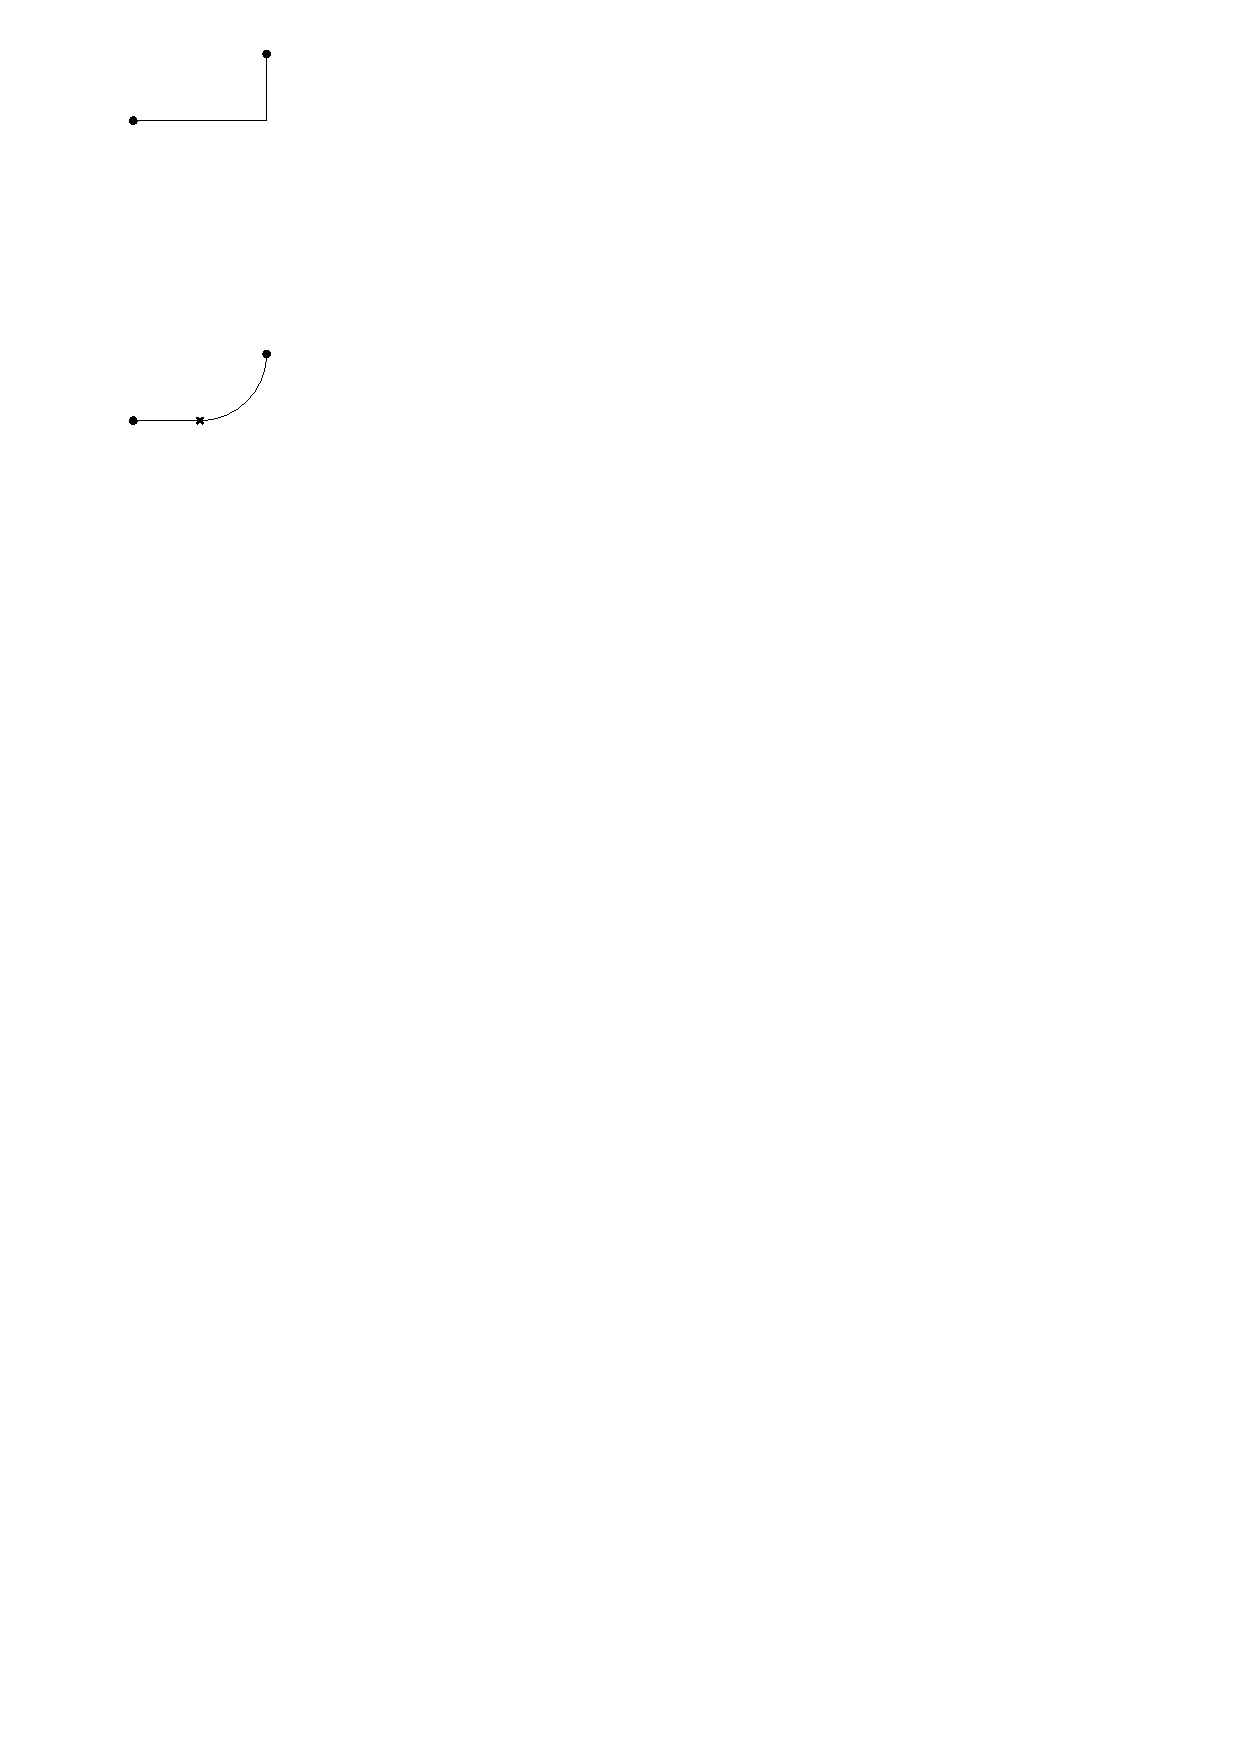
\includegraphics[scale=.8]{sc2_conversion/LEdge}}
        \subcaptionbox{U/C"~Kante\label{fig:sc2conversionUCEdge}}
            {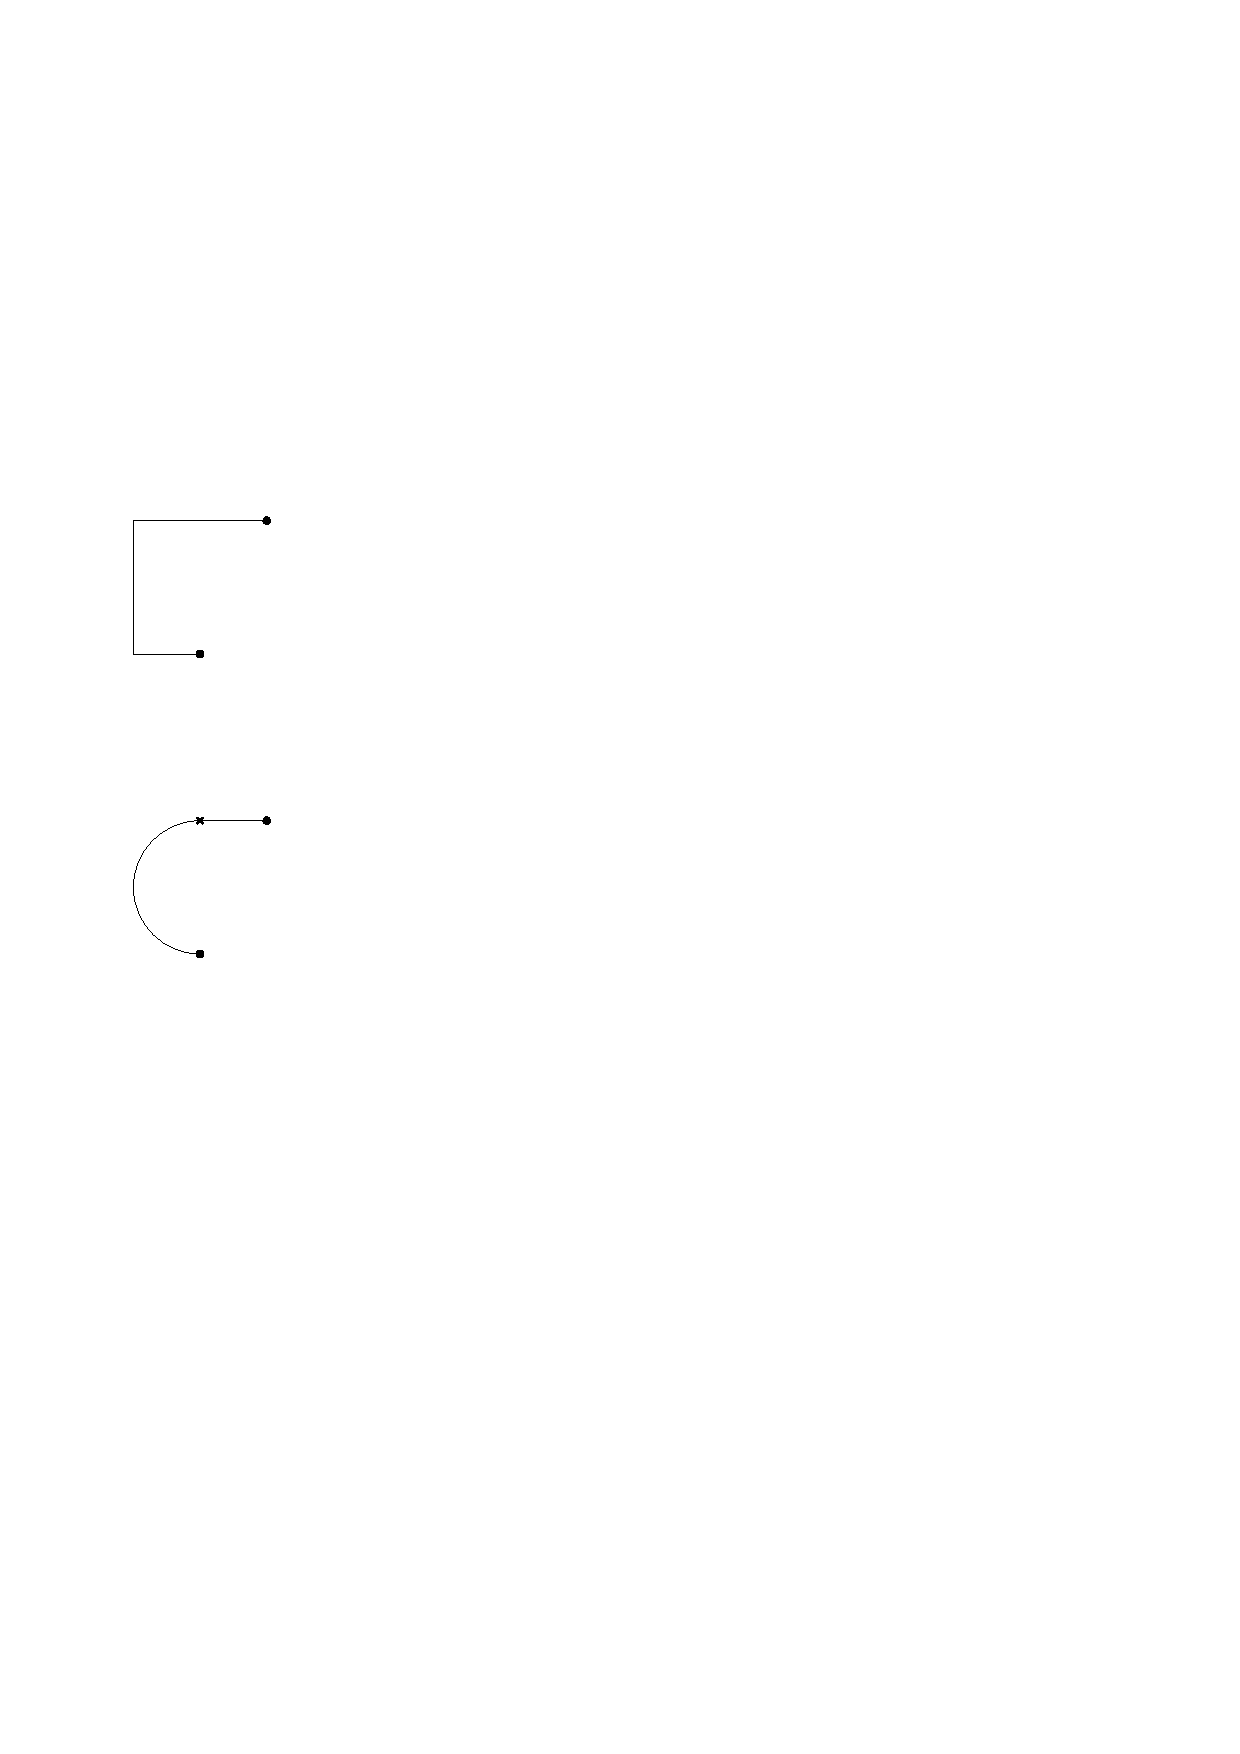
\includegraphics[scale=.8]{sc2_conversion/UCEdge}}
        \quad
        \subcaptionbox{S"~Kante\label{fig:sc2conversionSEdge}}
            {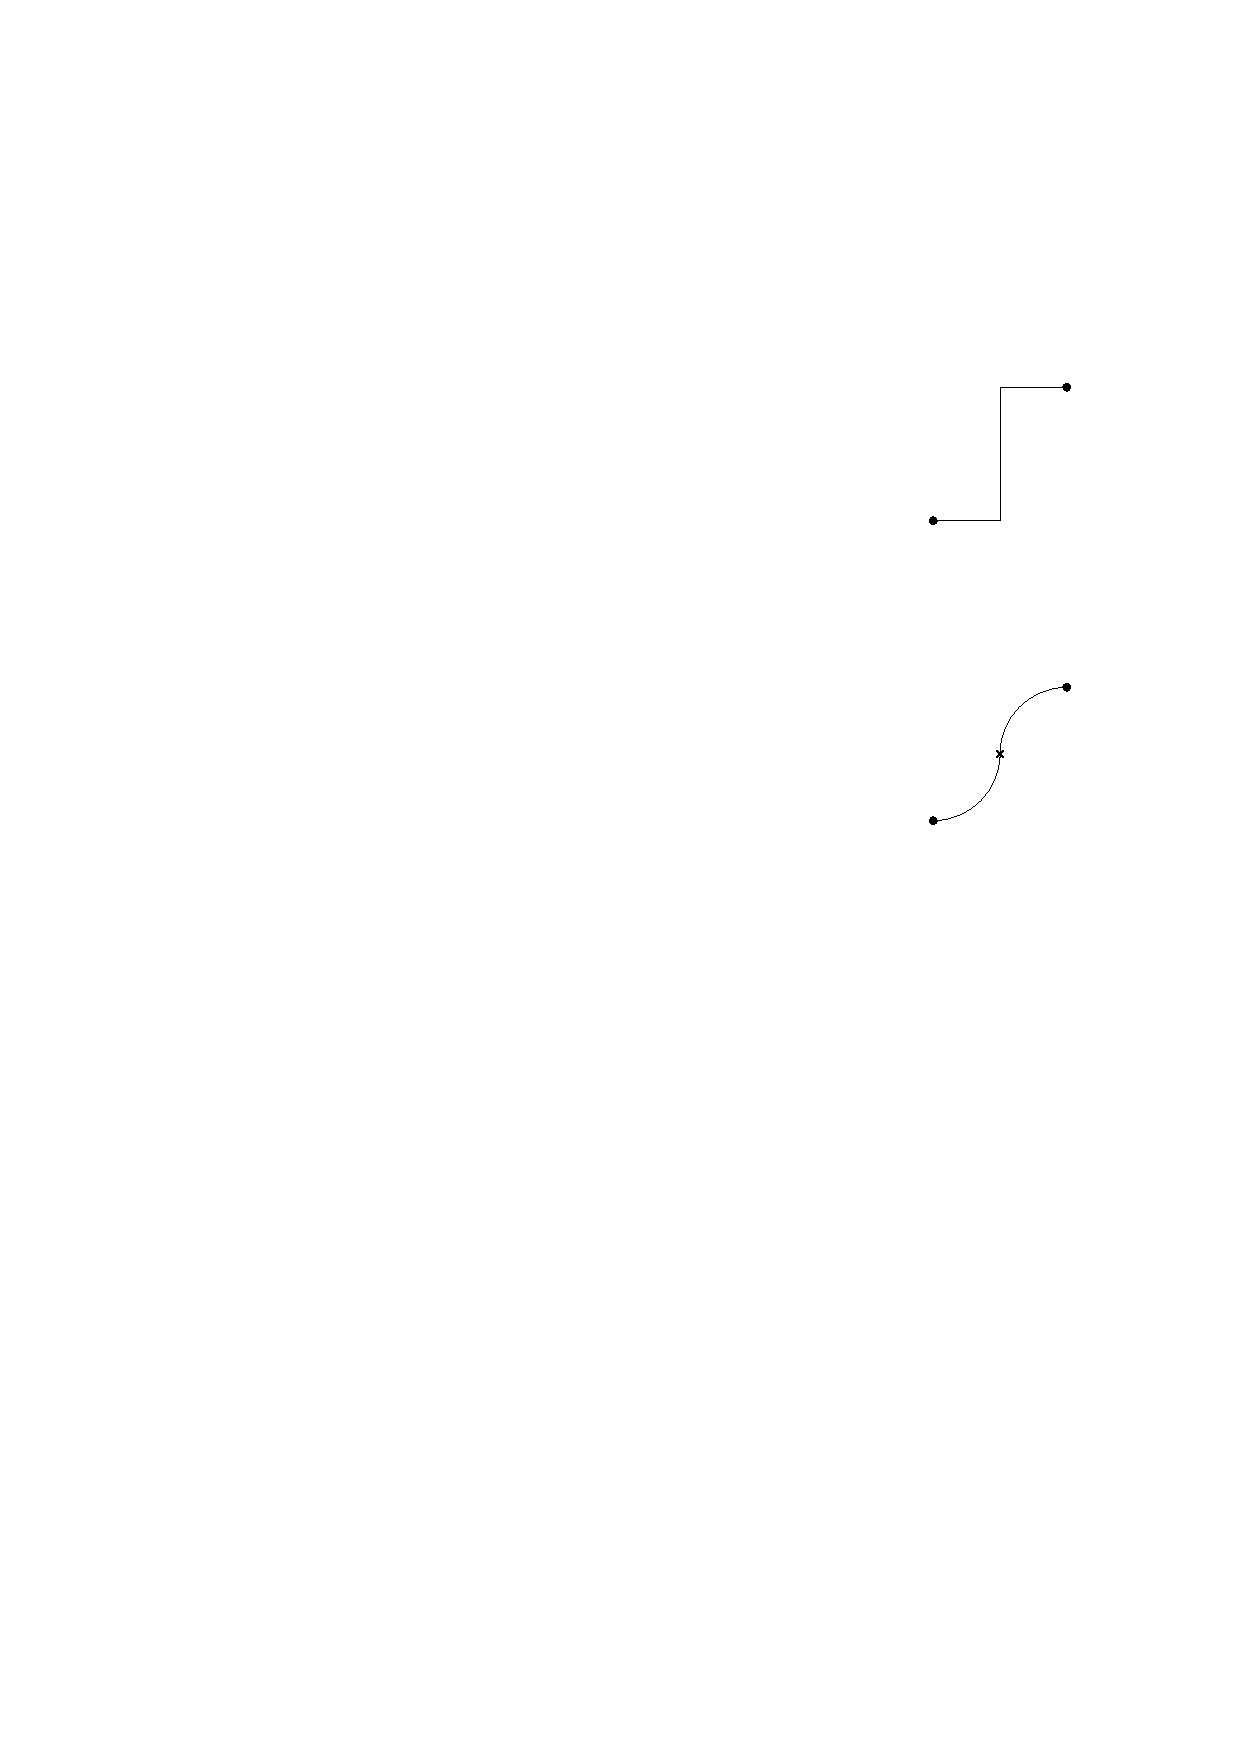
\includegraphics[scale=.8]{sc2_conversion/SEdge}}
        \quad
        \subcaptionbox{G"~Kante\label{fig:sc2conversionGEdge}}
            {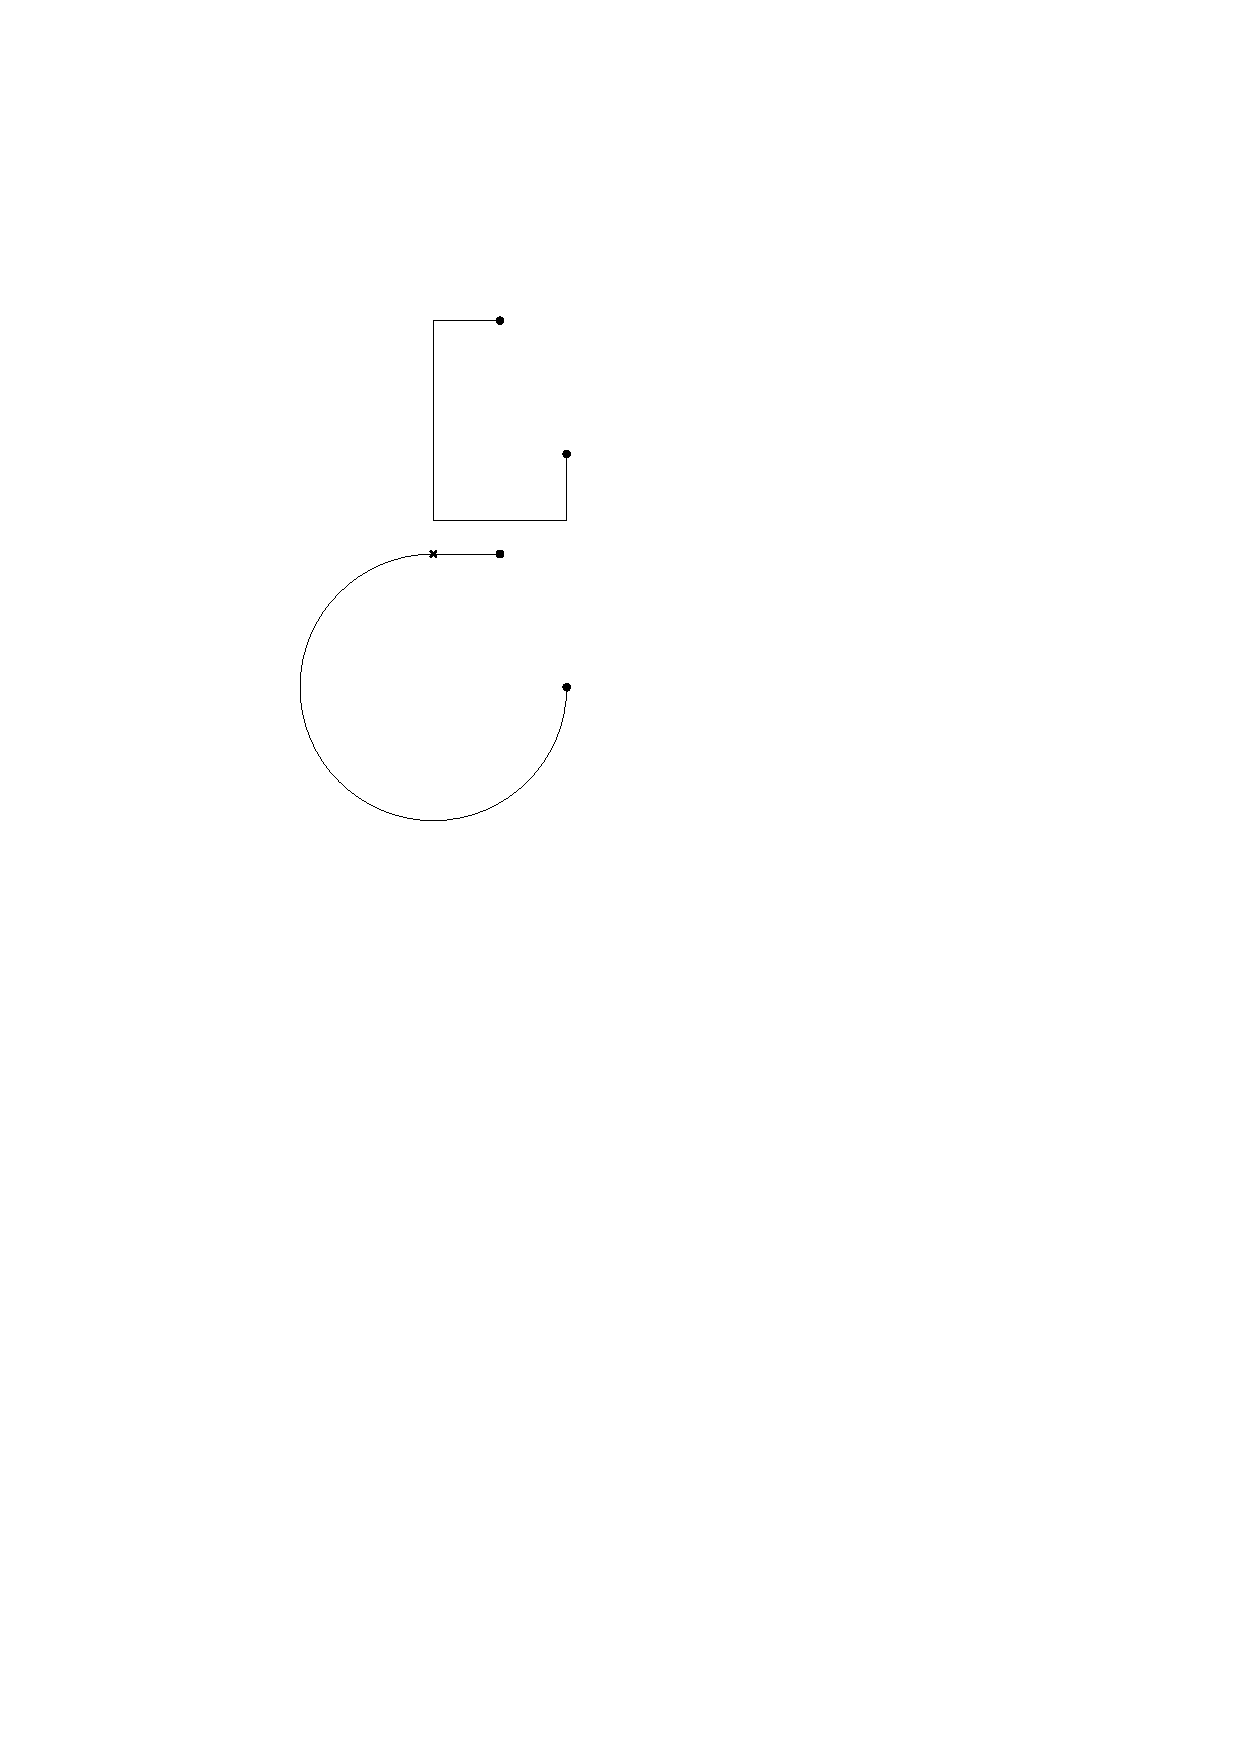
\includegraphics[scale=.8]{sc2_conversion/GEdge}}
        \quad

        \caption{Konvertierung von orthogonalen Kanten (oben) mit maximaler Komplexität~3 und einer Kante mit Komplexität~4 bei \ref{fig:sc2conversionGEdge} in glatt"=orthogonale Kanten (unten) mit maximaler Komplexität~2. Nicht gezeigt sind Drehungen und Spiegelungen dieser Beispiele.}
        \label{fig:sc2conversion}
\end{figure}

Es sollen alle Fälle für das Aussehen einer orthogonalen Kante behandelt werden. Da es in einem OC$_3$-Layout nur maximal drei Segmente geben kann, und zwei horizontale/vertikale Segmente hintereinander ein horizontales/vertikales Segment bilden würden, gibt es nicht sehr viele Möglichkeiten für die Anordnung der Segmente, insbesondere da gedrehte und gespiegelte Anordnungen zusammenzufassen sind.

Kanten mit einem Segment sind entweder horizontal oder vertikal. Diese können unverändert als Liniensegment in eine glatt"=orthogonale Zeichnung übernommen werden und sie werden nach ihrem Aussehen \emph{I"~Kanten} genannt.

Kanten mit zwei Segmenten bestehen aus einem horizontalen und einem vertikalen Segment. In der glatt"=orthogonalen Zeichnung werden diese mit einem Viertelkreis und, falls nötig, einem Liniensegment gezeichnet. Sie werden nach ihrem Aussehen \emph{L"~Kanten} genannt. Ist ihre Steigung größer als 45\textdegree, so hat die L"~Kante ein vertikales Liniensegment, ansonsten ein horizontales.

Kanten mit drei Segmenten bestehen aus einem horizontalem Segment zwischen zwei vertikalen Segmenten oder umgekehrt. Hier gibt es zwei verschiedene Fälle: Die äußeren Segmente können in dieselbe Richtung zeigen. Dann werden sie mit einem Halbkreis und, falls nötig, einem Liniensegment gezeichnet. Diese Kanten werden \emph{U"~}~oder \emph{C"~Kante} genannt, je nachdem, ob die Ports horizontal oder vertikal sind.

Zeigen die äußeren Segmente in verschiedene Richtungen, ergibt sich eine \emph{S"~Kante} aus zwei Kreissegmenten. Nur wenn die Steigung 45\textdegree\ beträgt, ist die Tangente am Segmentwechsel parallel zu einer der Koordinatenachsen. S"~Kanten kommen bei der ersten Umsetzung ins SC$_2$-Layout nicht vor.

Eine weitere Kantenart kommt noch vor: An $v_1$ und $v_n$ kann es eine Kante mit drei Knicken geben. Diese werden durch ein 270\textdegree-Kreissegment und, falls nötig, ein Liniensegment gezeichnet und \emph{G"~Kante} genannt. Obwohl die Kante im orthogonalen Layout eine Komplexität~3 hat, kann sie in der glatt"=orthogonalen Zeichnung mit zwei Segmenten dargestellt werden.

Eine Übersicht des Verfahrens zeigt Abbildung~\ref{fig:sc2conversion}. Durch diese Zeichenvorschriften ist das Aussehen der Kanten festgelegt und in der Zeichnung können Überschneidungen dieser Kanten erkannt werden, um eine planare Zeichnung zu erhalten.

\section{Entfernen von Überschneidungen im SC$_2$-Layout}
\label{sec:sc2makePlanarAlgo}

In der letzten Iteration wurde ein OC$_3$-Layout ohne stufenförmige Kanten erstellt. Dieses soll nun in ein SC$_2$-Layout konvertiert werden. Dabei wird die Portzuweisung nicht geändert, sodass sich auch die planare Einbettung nicht ändert. Problematisch sind jedoch die glatt"=orthogonalen Kanten, die anders geformt sind und sich überschneiden können, wenn die Knoten-Positionen aus dem OC$_3$-Layout benutzt werden. Darum sollen jetzt die Knotenpositionen so angepasst werden, dass es nicht mehr zu Überschneidungen kommt.

Während schrittweise das SC$_2$-Layout von unten nach oben aufgebaut wird, sollen stets alle L"~Kanten ein horizontales Liniensegment haben, niemals aber ein vertikales Liniensegment. Das horizontale Liniensegment kann die Länge~0 haben.

Bei der Entfernung der stufenförmigen Kanten wurden die Knoten in Plateaus gruppiert. Die Plateaus werden nun von unten nach oben durchlaufen und nacheinander in einem neuen Layout platziert. Abweichend von Alam et al.~\cite{smooth-13} können mehrere Plateaus dieselbe Höhe erhalten.

Dazu wird zunächst der erste Knoten ganz links im Plateau platziert und der letzte Knoten ganz rechts im Plateau. Es ist möglich, dass dies ein und derselbe Knoten ist. Beide Knoten werden wieder in der Spalte der Kante an ihren unteren Ports platziert, sowie auf der Höhe des Plateaus. Danach werden die ausgehenden Kanten platziert: Die Kanten bekommen relativ zu den Knoten die selbe x"~Koordinate wie im OC$_3$-Layout. Die y"~Koordinate aller offenen Kanten sei die y"~Koordinate des aktuellen Plateaus. 

\begin{figure}[h]
        \centering
       \subcaptionbox{Anpassungen der Kontenpositionen, um Kollisionen mit einer neuen C"~Kante zu vermeiden.\label{fig:accomodateCedge} }[.28\textwidth]
            {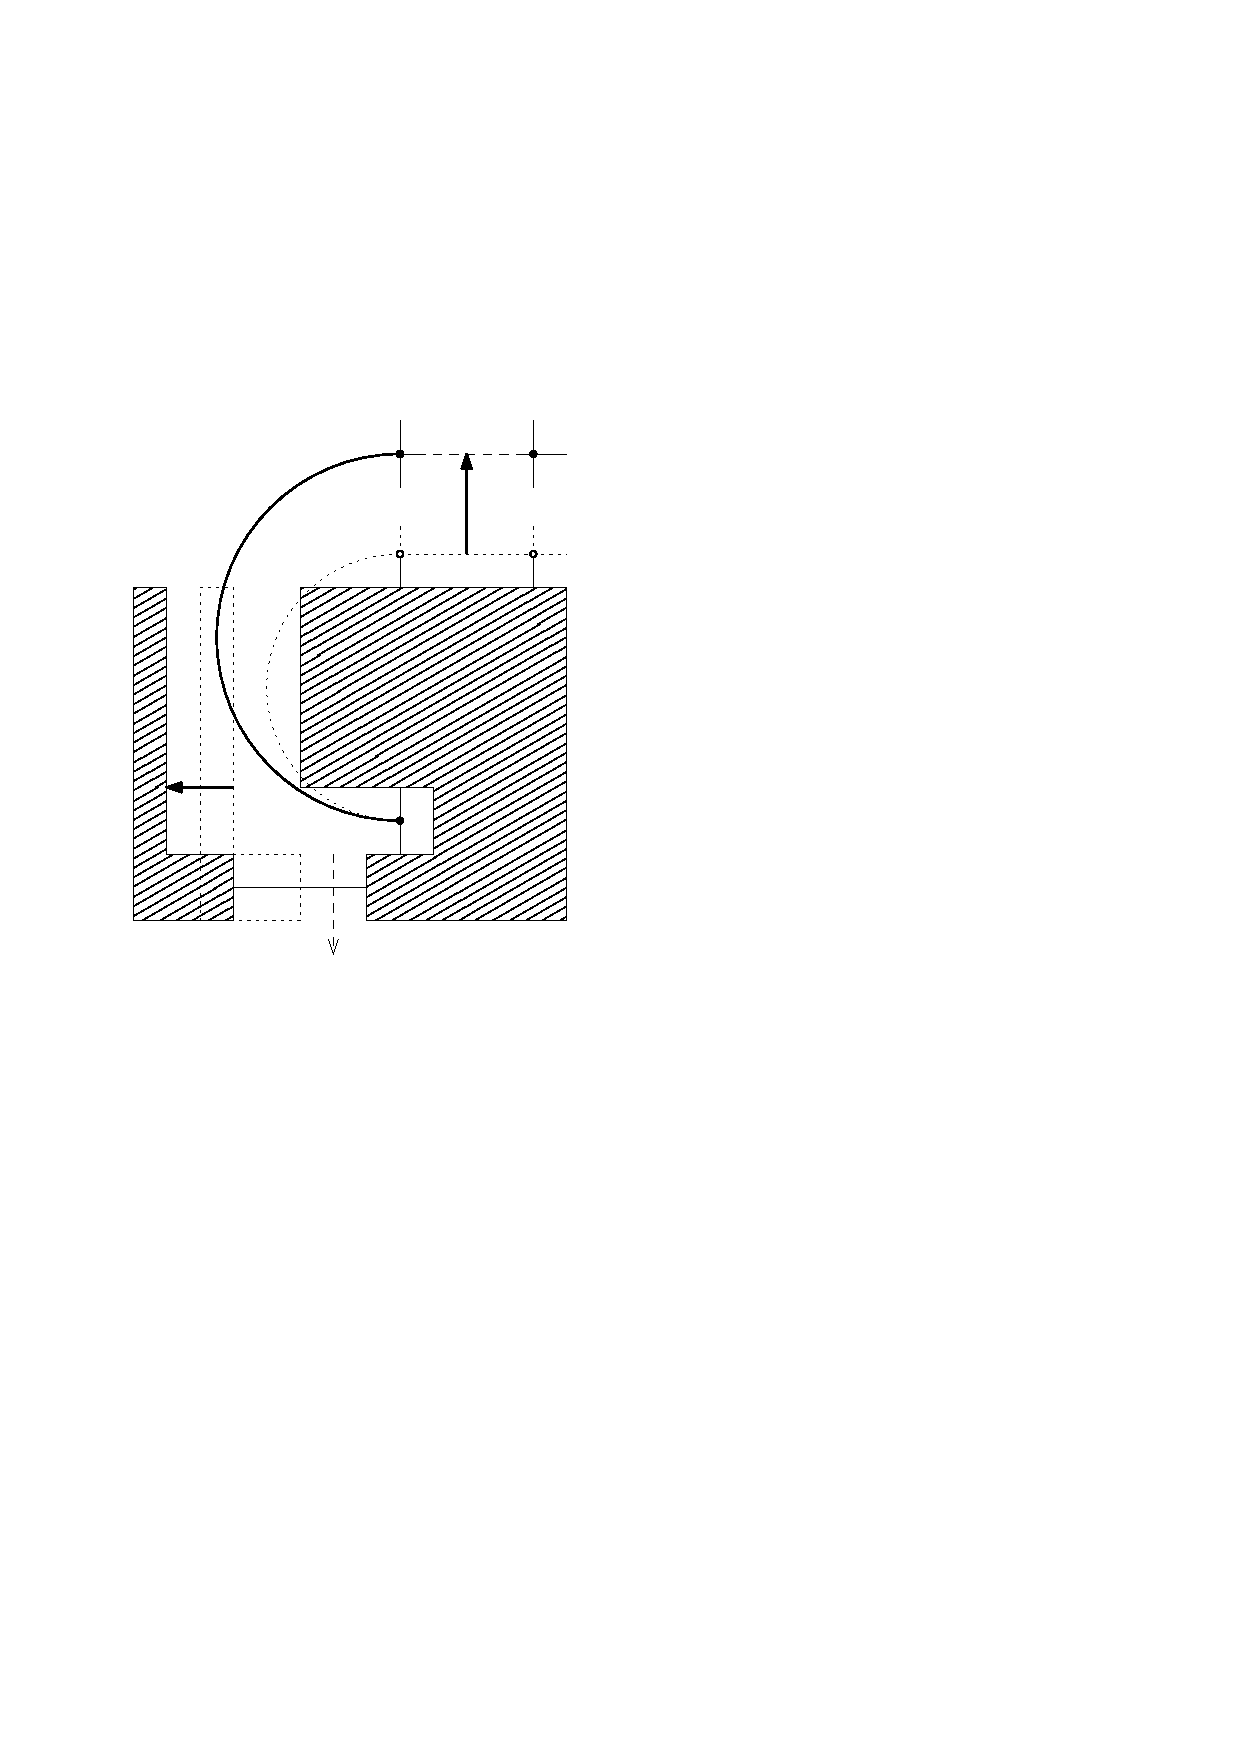
\includegraphics[width=.28\textwidth]{accomodate_C_edge}}
        \quad
       \subcaptionbox{Finden eines Schnittes zum Trennen des Graphen in eine linke und einer rechte Seite. Die linke Seite und der untere Knoten können frei nach links verschoben werden, um die Steigung der L"~Kante zu korrigieren.\label{fig:cutLslopecorrection} }[.68\textwidth]
            {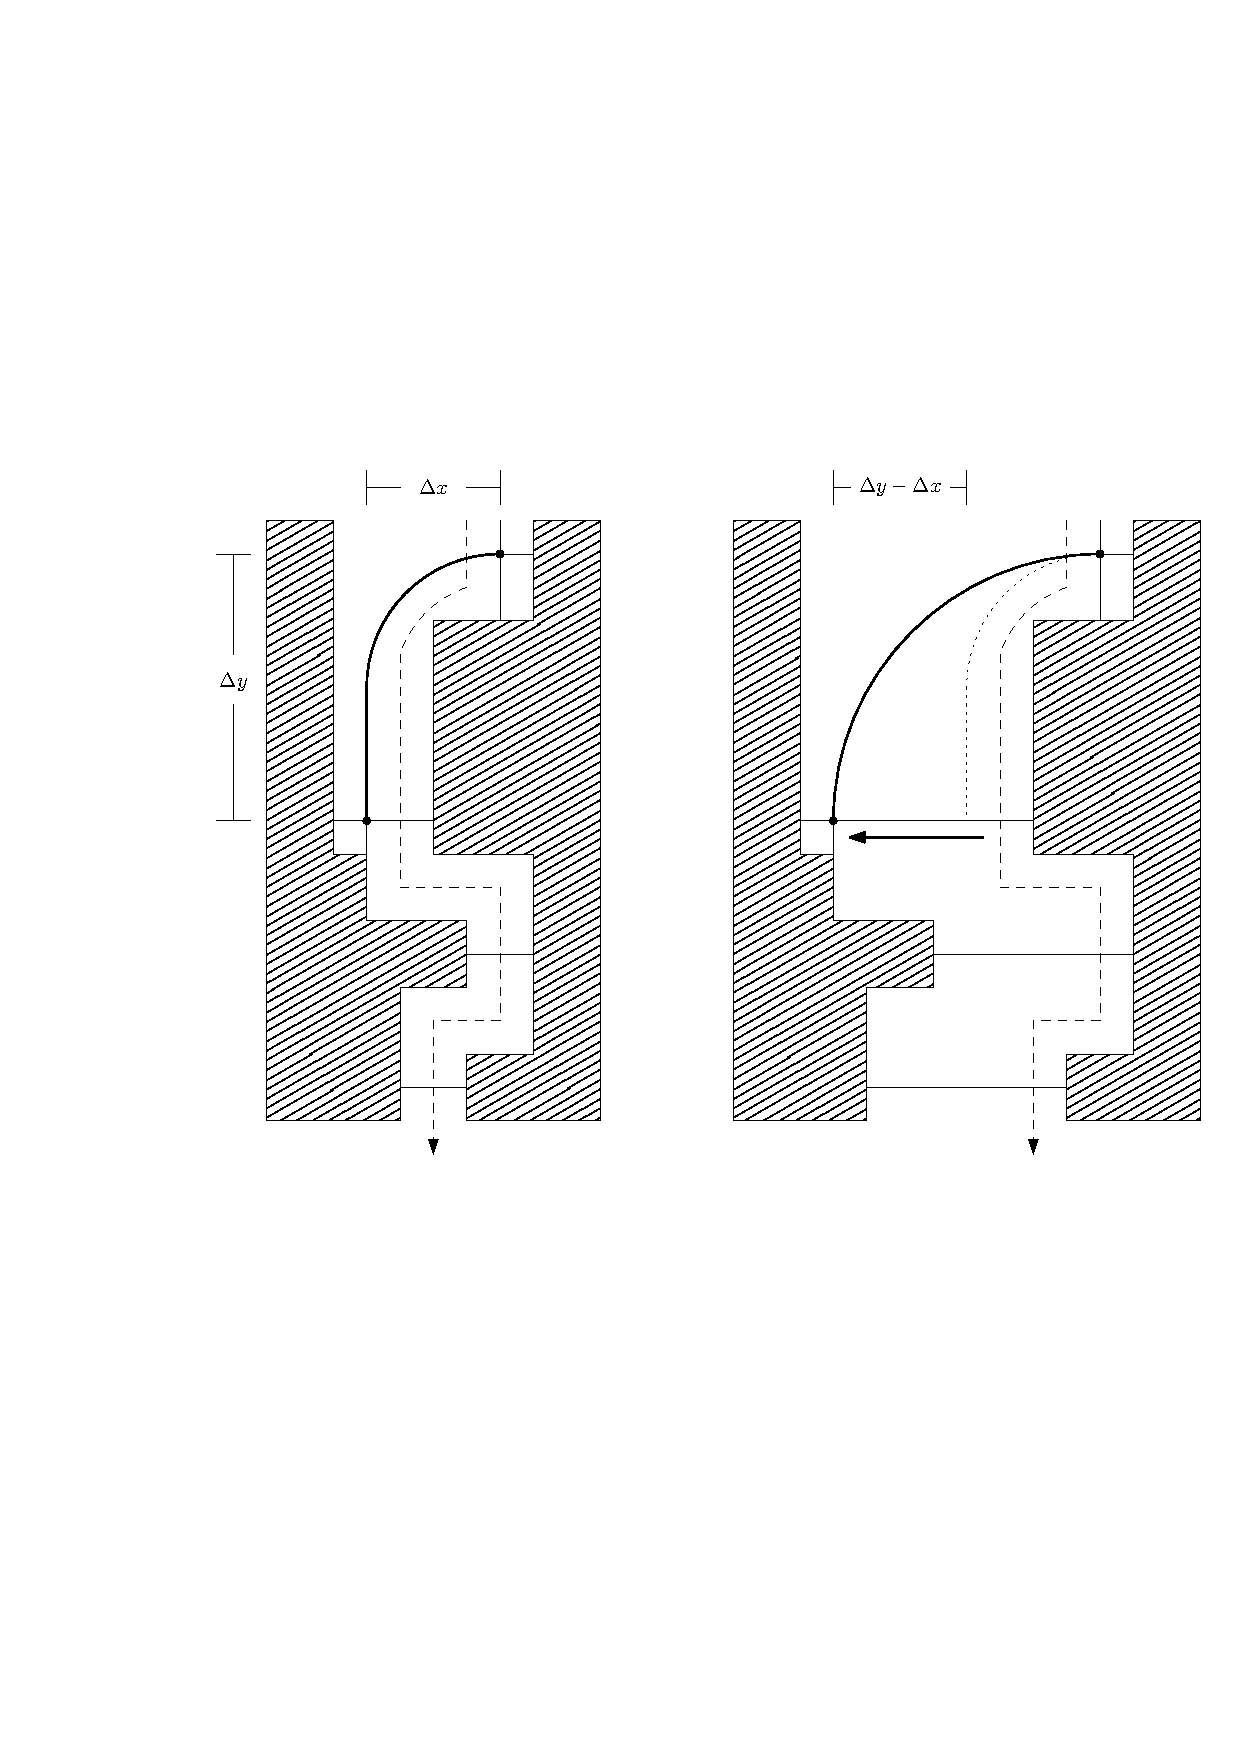
\includegraphics[width=.68\textwidth]{cut_L_slope_correction}}
 
        \caption{Maßnahmen zur Vermeidung von Kollisionen: Verschieben von Knoten zur Kollisionsvermeidung (\subref{fig:accomodateCedge}) und Korrektur der Steigung (\subref{fig:cutLslopecorrection}). Mit Schraffur gefüllte Blöcke stehen für Teile des Graphen in der Zeichnung, deren genaues Aussehen nicht relevant ist, gestrichelt sind die Schnitte und gepunktet Positionen vor der Anpassung.}
        \label{fig:collisionAvoidanceAndSlopeCorrection}
\end{figure}

Nun werden Überschneidungen mit der Kante $e_\text{l}$ am linken Port des ersten Knotens und der Kante $e_\text{r}$ am rechten Port des letzten Knotens aufgelöst. Gibt es jeweils an dem Port keine Kante, entfallen die entsprechenden Anpassungen. Zuerst werden innere Überschneidungen mit Kanten rechts der Kante $e_\text{l}$  und links der Kante $e_\text{r}$ behoben: Das gesamte Plateau und alle Plateaus darüber werden so lange nach oben verschoben, bis es keine Kollision mit inneren Kanten mehr gibt. In Abbildung~\ref{fig:accomodateCedge} kollidiert der rechte Block innen mit der C"~Kante und das Plateau wird nach oben verschoben.

Dann werden äußere Überschneidungen mit Kanten links von $e_\text{l}$ behoben: Von leicht links des unteren Knoten von  $e_\text{l}$ aus nach unten wird der Graph in eine rechte und eine linke Seite geteilt, und zwar so, dass der Schnitt nur durch horizontale Liniensegmente, G"~, U"~~oder offene Kanten führt. Die linke, abgeschnittene Seite des Graphen wird dann nach links verschoben, bis es keine Kollision mit $e_\text{l}$ mehr gibt. Die horizontalen Segmente werden dadurch länger. In Abbildung~\ref{fig:accomodateCedge} ist der Schnitt und das Verschieben der linken Seite exemplarisch dargestellt. Wenn die Kante $e_\text{l}$ eine L"~Kante ist, muss noch die Steigung angepasst werden, falls sie ein vertikales Liniensegment hat. Dazu wird leicht rechts des unteren Knotens ein Schnitt nach unten begonnen und dann alles links des Schnitts so weit nach links verschoben, dass die Kante kein vertikales Liniensegment mehr hat. Dies wird in Abbildung~\ref{fig:cutLslopecorrection} gezeigt. Dann wird für $e_\text{r}$ die Entfernung der Überschneidungen und die Korrektur der Steigung analog, also horizontal gespiegelt, durchgeführt.

Alam et al.~\cite{smooth-13} achten im Verlauf des Algorithmus darauf, C"~Kanten mit horizontalen Segmenten am oberen Knoten zu vermeiden. Es zeigte sich uns jedoch keine Möglichkeit auf, wie diese Methodik korrekt anzuwenden ist, da bei der beschriebenen Methode mit Schnitten durch vertikale Segmente zu rechnen ist. Problematisch ist der Fall, wenn ein Schnitt rechts am oberen Knoten vorbei läuft und dann die Kante links am unteren Knoten durchschneidet, falls hier kein horizontales Segment ist, das verlängert werden kann. Am oberen Knoten befindet sich dann ein horizontales Segment und beim Bewegen des unteren Knotens bewegt sich die C"~Kante fälschlicherweise mit oder erhält ein drittes Segment. Es wurde unter anderem versucht zu beweisen, dass solch ein Schnitt mit den bestehenden Regeln nicht möglich ist, was jedoch scheitert, wenn eine weitere C"~Kante in den Innenbereich der C"~Kante ragt, an der der Schnitt entlang geführt werden könnte. An dieser Stelle bleibt es offen, hierfür eine sorgfältige Lösung zu erarbeiten.

% TODO: G"~Kanten-Korrektur

Abweichend von Alam et al.~\cite{smooth-13} prüfen wir die Überschneidungen mit inneren Kanten des letzten Knotens, bevor die Steigung der Kanten angepasst wird, denn wenn der letzte Knoten mit dem gesamten Plateau nach oben verschoben wird, kann die Steigung von $e_\text{l}$ über 45\textdegree\ steigen. Zudem haben wir das Finden des Schnitts leicht verändert, was in Abschnitt \ref{sec:cutfinding} näher erläutert wird. Außerdem verschieben wir zur Anpassung der Steigung nur genau so weit, wie nötig, um die Steigung auf 45\textdegree\ zu senken: $\Delta y - \Delta x$.

Jetzt werden die übrigen Knoten mit ihren offenen Kanten platziert. Daraufhin müssen noch die Kanten an den unteren Ports auf Kollisionen überprüft werden. Hier kann es zu Überschneidungen kommen, wenn es L"~Kanten sind. Hierbei beginnt der Schnitt leicht unterhalb des Knotens auf der Seite, in die die L"~Kante zeigt. Dann wird die L"~Kante durchschnitten und der restliche Graph unterhalb geteilt, wobei wiederum nur horizontale Liniensegmente durchquert werden. Dann wird der Teil der Zeichnung des Graphen auf der Seite, in die die L"~Kante zeigt, noch weiter in die Richtung der L"~Kante verschoben, bis es keine Überschneidungen mehr gibt und die L"~Kante eine Steigung kleiner als 45\textdegree\ hat. Dieser Schritt findet sich bei Alam et al.~\cite{smooth-13} nicht und wurde hinzugefügt, nachdem sich sonst ungelöste Überschneidungen ergeben haben.

Offene Kanten haben noch keine festgelegte Form, bis ihr zweiter Knoten auch platziert wurde. Zur Kollisionserkennung behandeln wir sie als vertikale Linien mit der x"~Koordinate der Spalte der Kante. Die Linien reichen von der x"~Koordinate des ersten Knotens bis über die Höhe des gerade zu platzierenden Plateaus. Die Behandlung der offenen Kanten wurde bei Alam et al.~\cite{smooth-13} nicht weiter spezifiziert, jedoch müssen sie in die Kollisionserkennung einbezogen werden, da sonst vertikale Liniensegmente keiner Überschneidungsvermeidung unterliegen und mit C"~Kanten kollidieren.

Wenn alle Plateaus vollständig platziert sind, ist das neue Layout eine glatt"=orthogonale und planare Version des OC$_3$-Layouts, mit denselben Portzuweisungen und der selben planaren Einbettung. Damit verbleibt nur noch, das Layout in eine Zeichnung zu überführen. 

%\section{Zusammenfassung}
% TODO: explain whats missing


\chapter{Implementierung}
\label{chap:impl}

Im Kapitel~\ref{chap:algo} wurde das Grundgerüst des Algorithmus beschrieben. Einige Teile des Algorithmus wurden nur sehr grobkörnig beschrieben, gerade so, dass es für das Verständnis und die Nachvollziehbarkeit reicht, aber nicht genau genug für eine Implementierung. Diese Teile sollen nun hier im Detail erklärt werden. Zudem werden einige Implementierungsdetails aufgeführt, die sich für ähnliche Implementierungs-Projekte nützlich erweisen sollten.

\section{Software}

Für die Implementierung in der Programmiersprache \emph{Java} wurde, wo möglich, auf bestehende und bewährte Software-Grundlagen gesetzt.

Das Ausgangsformat, aus dem die Graphen eingelesen wurde, ist \emph{GraphML}~\cite{brandes+al-14}. Das freie Datenformat ist das Ergebnis von Bemühungen, ein standardisiertes Format für das Speichern von Graphen zu schaffen. Es basiert auf XML, kann alle Arten von Graphen speichern und ist zudem um eigene Attribute erweiterbar, diese Erweiterungen können beim Einlesen übersprungen werden.

Die Eingabedaten für die Graphen stammen größtenteils aus den \emph{Rom-Testgraphen}\footnote{Erhältlich unter \url{http://www.graphdrawing.org/data/}}, einer Sammlung von verschiedensten Graphen mit 10 bis 100 Knoten im GraphML-Format. Für das schelle Erstellen von Testgraphen für einige Spezialfälle wurde der Grapheneditor \emph{yEd}\footnote{Erhältlich unter \url{http://www.yworks.com/de/products_yed_about.html}} von yWorks verwendet, der ebenfalls das GraphML-Format unterstützt und Graphen übersichtlich visualisieren kann.

Zum Einlesen der Graphen in Java und ihre Repräsentation im Speicher wurde \emph{JUNG}\footnote{Erhältlich unter \url{http://jung.sourceforge.net/}}, das \emph{Java Universal Network/Graph Framework}~\cite{jung}, verwendet. Es beinhaltet neben effizienten Implementierungen von verschiedenen Graphen, etwa gerichtete und ungerichtete, einige Algorithmen auf Graphen und Werkzeuge zur Visualisierung. Außerdem lassen sich damit GraphML-Dateien einlesen.

Die Ausgabe der fertigen Zeichnungen erfolgte im Vektorgrafik-Format des Editors \emph{Ipe}\footnote{Erhältlich unter \url{http://ipe7.sourceforge.net/}}. Das Format basiert auf XML und erhält Möglichkeiten für das Zeichnen von Punkten, Linien und Kreisbögen und vielem mehr. Der Vorteil gegenüber anderen Vektorformaten ist, dass sich \LaTeX-Beschriftungen in den Zeichnungen platzieren lassen und die Zeichnungen in PDF-Dateien konvertiert werden können. Die fertigen Zeichnungen können mit dem Ipe-Editor annotiert und weiter bearbeitet werden.

Zum Erstellen der Ipe-Dateien aus Java wurde die \emph{IpeDraw-Bibliothek}\footnote{Erhältlich unter \url{http://lamut.informatik.uni-wuerzburg.de/mediawiki/ipe7/index.php/JAVAtoIPE}} von Philipp Kindermann und Martin Fink verwendet.

Es wurden also Daten aus dem Rom-Testgraphen entnommen oder direkt in yEd erstellt, in Java mittels JUNG eingelesen, durch den Algorithmus visualisiert und mit der IpeDraw-Bibliothek als Vektorgrafiken ausgegeben, welche im Ipe-Editor betrachtet werden können oder in PDFs konvertiert werden.

\section{Zeichnen der glatt"=orthogonalen Kanten}

In Abschnitt~\ref{sec:sc2conversion} wurde bereits beschrieben, wie eine orthogonale Kanten in eine glatt"=orthogonale Kante konvertiert werden kann. Zu diesen Konversionsvorschriften wurde im Rahmen der Arbeit ein Algorithmus entwickelt, der anhand der Portzuweisung und der relativen Position der Knoten die Form der Kante und die Position des Segmentwechsels berechnen kann. 

Der erste Schritt ist eine Fallunterscheidung nach den beiden Ports, mit denen die Kante verbunden ist. Liegen die Ports gegenüber, so muss eine I"~~oder S"~Kante vorliegen. Sind beide Ports vertikal oder beide horizontal, so liegt eine U"~~oder C"~Kante vor. Andernfalls liegt eine L- oder G"~Kante vor.

Liegt eine I"~Kante vor, müssen nur die beiden Knoten mit einer Linien verbunden werden. % TODO: S"~Kante

Liegt eine U"~Kante (C"~Kante) vor, so muss zunächst bestimmt werden, an welchem der beiden Endknoten das Liniensegment beginnt. Man kann ohne Beschränkung der Allgemeinheit annehmen, dass es immer ein Liniensegment gibt. Ist die Kante an den unteren (linken) Ports, so ist der Knoten weiter oben (rechts) der Startpunkt des Liniensegments, ansonsten der weiter unten (links). Die Position des Segmentwechsels hat nun die x"~Koordinate des anderen Punktes (dieses Startpunkts) und die y"~Koordinate dieses Startpunkts (des anderen Punktes). Der Mittelpunkt des Kreises ist der Punkt genau zwischen der Position des Segmentwechsels und des Startpunkts. Der Kreis muss im Uhrzeigersinn vom Startpunkt zum Segmentwechsel gezeichnet werden, wenn die Steigung der Geraden durch die zwei Knotenpositionen negativ (positiv) ist.

Liegt keine I"~, S"~, U"~~oder C"~Kante vor, so muss eine L-~oder G"~Kante vorliegen. Eine L"~Kante liegt je nach Ports und der Lage der Kantenendpunkte zueinander vor: Die Vorzeichen der Differenz der Richtungsvektoren der Ports an den Knoten müssen dieselben sein, wie die der Differenz der beiden Knotenpositionen. Bei L"~Kanten muss dann der Kreis im Uhrzeigersinn gezeichnet werden, wo er bei G"~Kanten gegen den Uhrzeigersinn gezeichnet wird und umgekehrt. Es gibt verschiedene Fälle: Koordinaten werden addiert oder subtrahiert, es gibt acht Port-Kombinationen, in denen dann L"~~oder G"~Kanten vorliegen und die relative Lage der beiden Knoten-Endpositionen kann in die vier Quadranten der Koordinatenebene fallen, über oder unter die entsprechende Diagonale.

Darum sei hier nur ein Beispielfall für eine Kante $\{v_1, v_2\}$ ausgeführt: Sei $v_2$ im ersten Quadranten und $v_1$ am Ursprung positioniert. Die ausschlaggebende Diagonale ist hier die Hauptdiagonale. Liegt nun $v_2$ oberhalb der Hauptdiagonale, so beginnt das Kreissegment bei $v_1$. Ansonsten beginnt es bei $v_2$. Sei nun also $v_2$ unterhalb der Hauptdiagonale. Dann muss die Differenz der y"~Koordinaten von der x"~Koordinate von $v_2$ abgezogen werden, um den Mittelpunkt des Kreises zu erhalten. Die Differenz muss von beiden Koordinaten von $v_2$ abgezogen werden, um die Position des Segmentwechsels zu erhalten. Die Kante besteht nun aus einer geraden Linie von $v_1$ zur Segmentwechselposition und einem Kreisbogen im Uhrzeigersinn von $v_2$ zur Segmentwechselposition. Die übrigen 63 Fälle überlegt man sich analog.

Mit diesen Schritten können für alle Kanten die Lage der Segmente und die Position des Segmentwechsels berechnet werden, anhand derer die Erkennung von Überschneidungen und das Realisieren der Zeichnung möglich ist.

\section{Schnitte finden}
\label{sec:cutfinding}

Das Finden eines Schnittes durch die Zeichnung des Graphen zum Zwecke des Verschiebens von Knoten in horizontale Richtung zielt darauf ab, den Graph in zwei Teile zu spalten, die nur durch horizontale Segmente verbunden sind. 

Der Schnitt beginnt oberhalb eines Knotens, entweder knapp links oder knapp rechts davon. Er setzt sich dann durch die Zeichnung fort und folgt dabei Kanten abwärts von Knoten zu Knoten. Er kann niemals vertikal oder nach oben verlaufen und ist somit \emph{y"~Monoton}. Dabei kann er C"~, I"~~und L"~Kanten an horizontalen Segmenten durchqueren, an diesen können sie beliebig auseinandergezogen werden. Zusätzlich kann er U"~~und G"~Kanten durchqueren. Diese Kantenarten treten nach Konstruktion nur an der Außenfacette des Graphen auf und ein Verändern der Knotenpositionen kann also keine neuen Überschneidungen nach sich ziehen. Niemals wird ein vertikales Liniensegment durchquert.

Hierbei ergeben sich verschiedene Fälle, die in Abbildung~\ref{fig:cutfinding} dargestellt sind. Dabei wird jeweils die Situation, dass der Schnitt auf der linken Seite eines Knotens $v$ beginnt, betrachtet, die andere Seite wird symmetrisch behandelt. 

\begin{figure}[h]
        \centering
        \begin{subfigure}[b]{0.2\textwidth}
                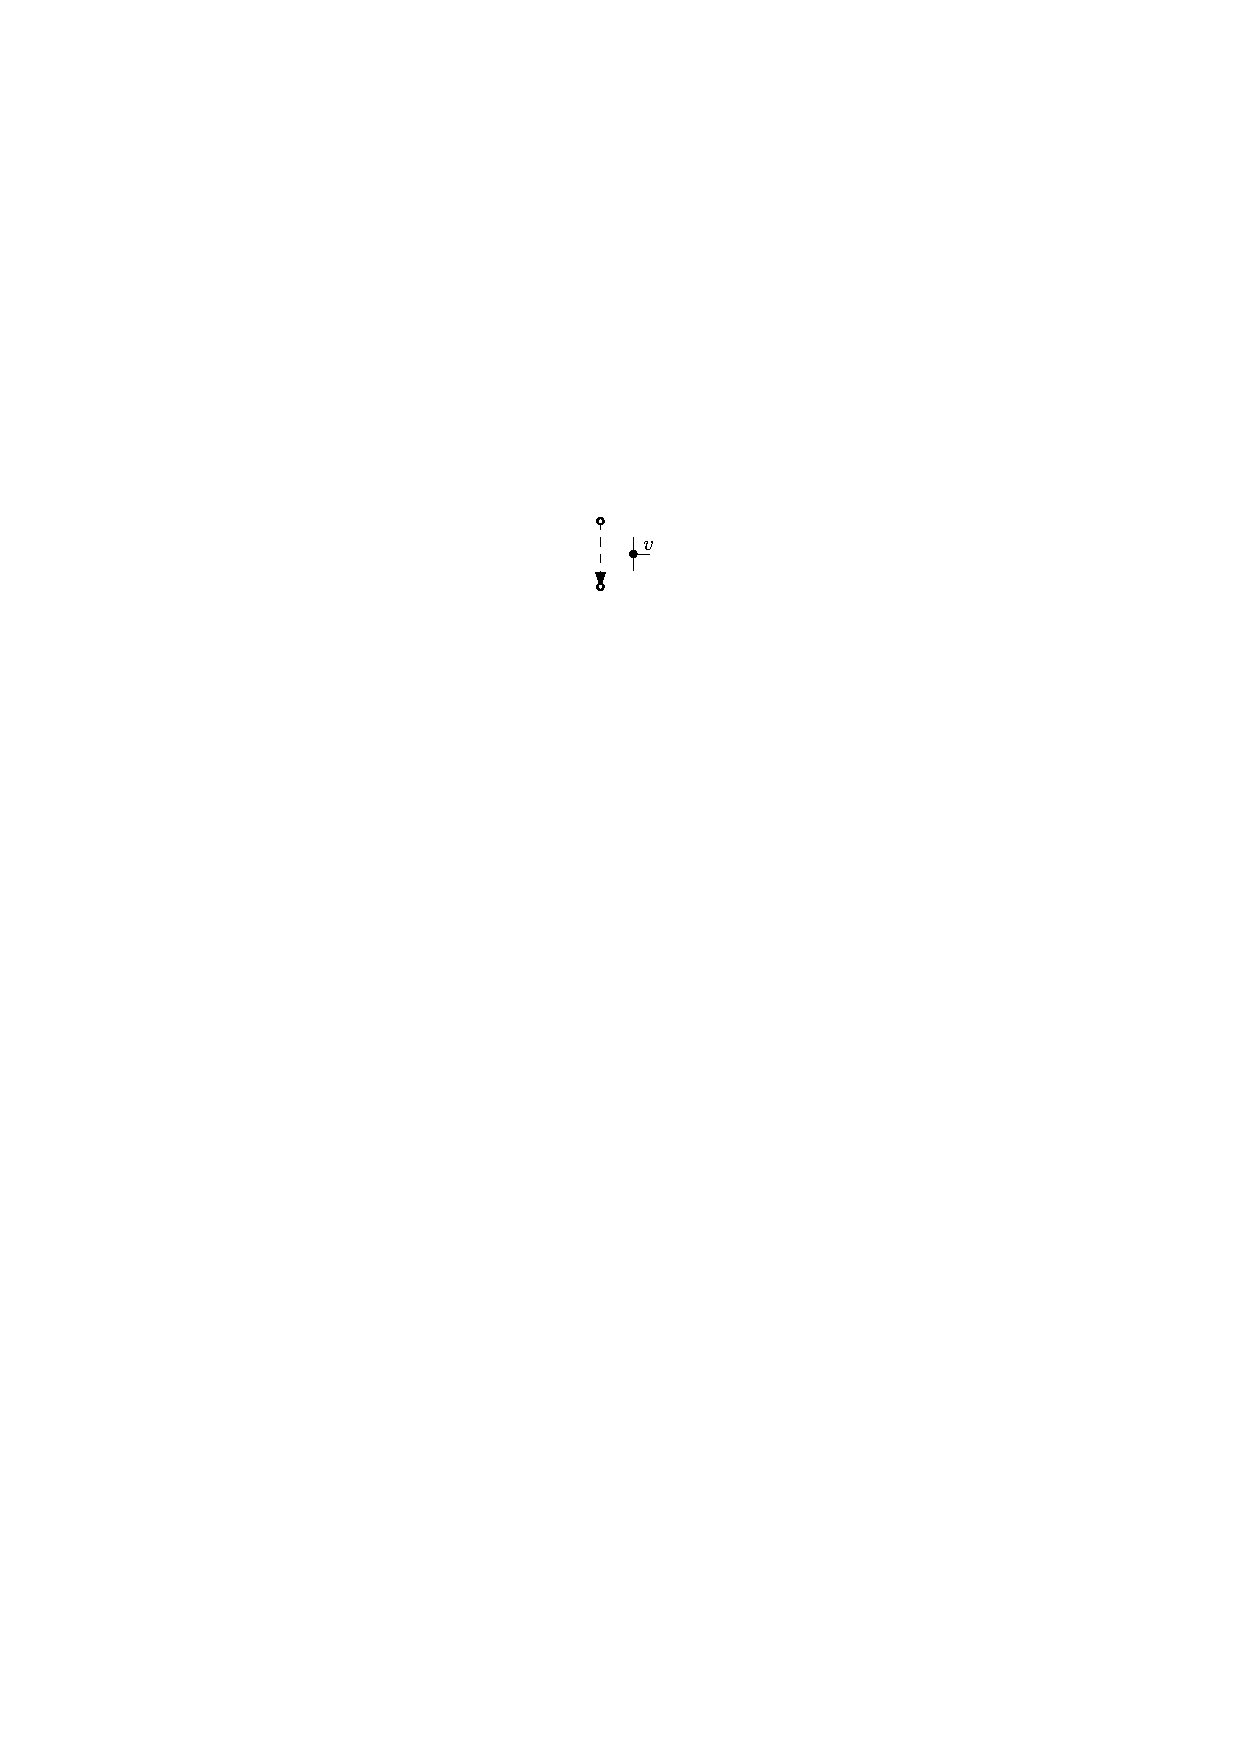
\includegraphics[width=0.5\textwidth]{schnitt_finden/top_none}
                \caption{Oberhalb,\\ keine Kante}
                \label{fig:cutfinding_top_none}
        \end{subfigure}%
        \quad
        \begin{subfigure}[b]{0.2\textwidth}
                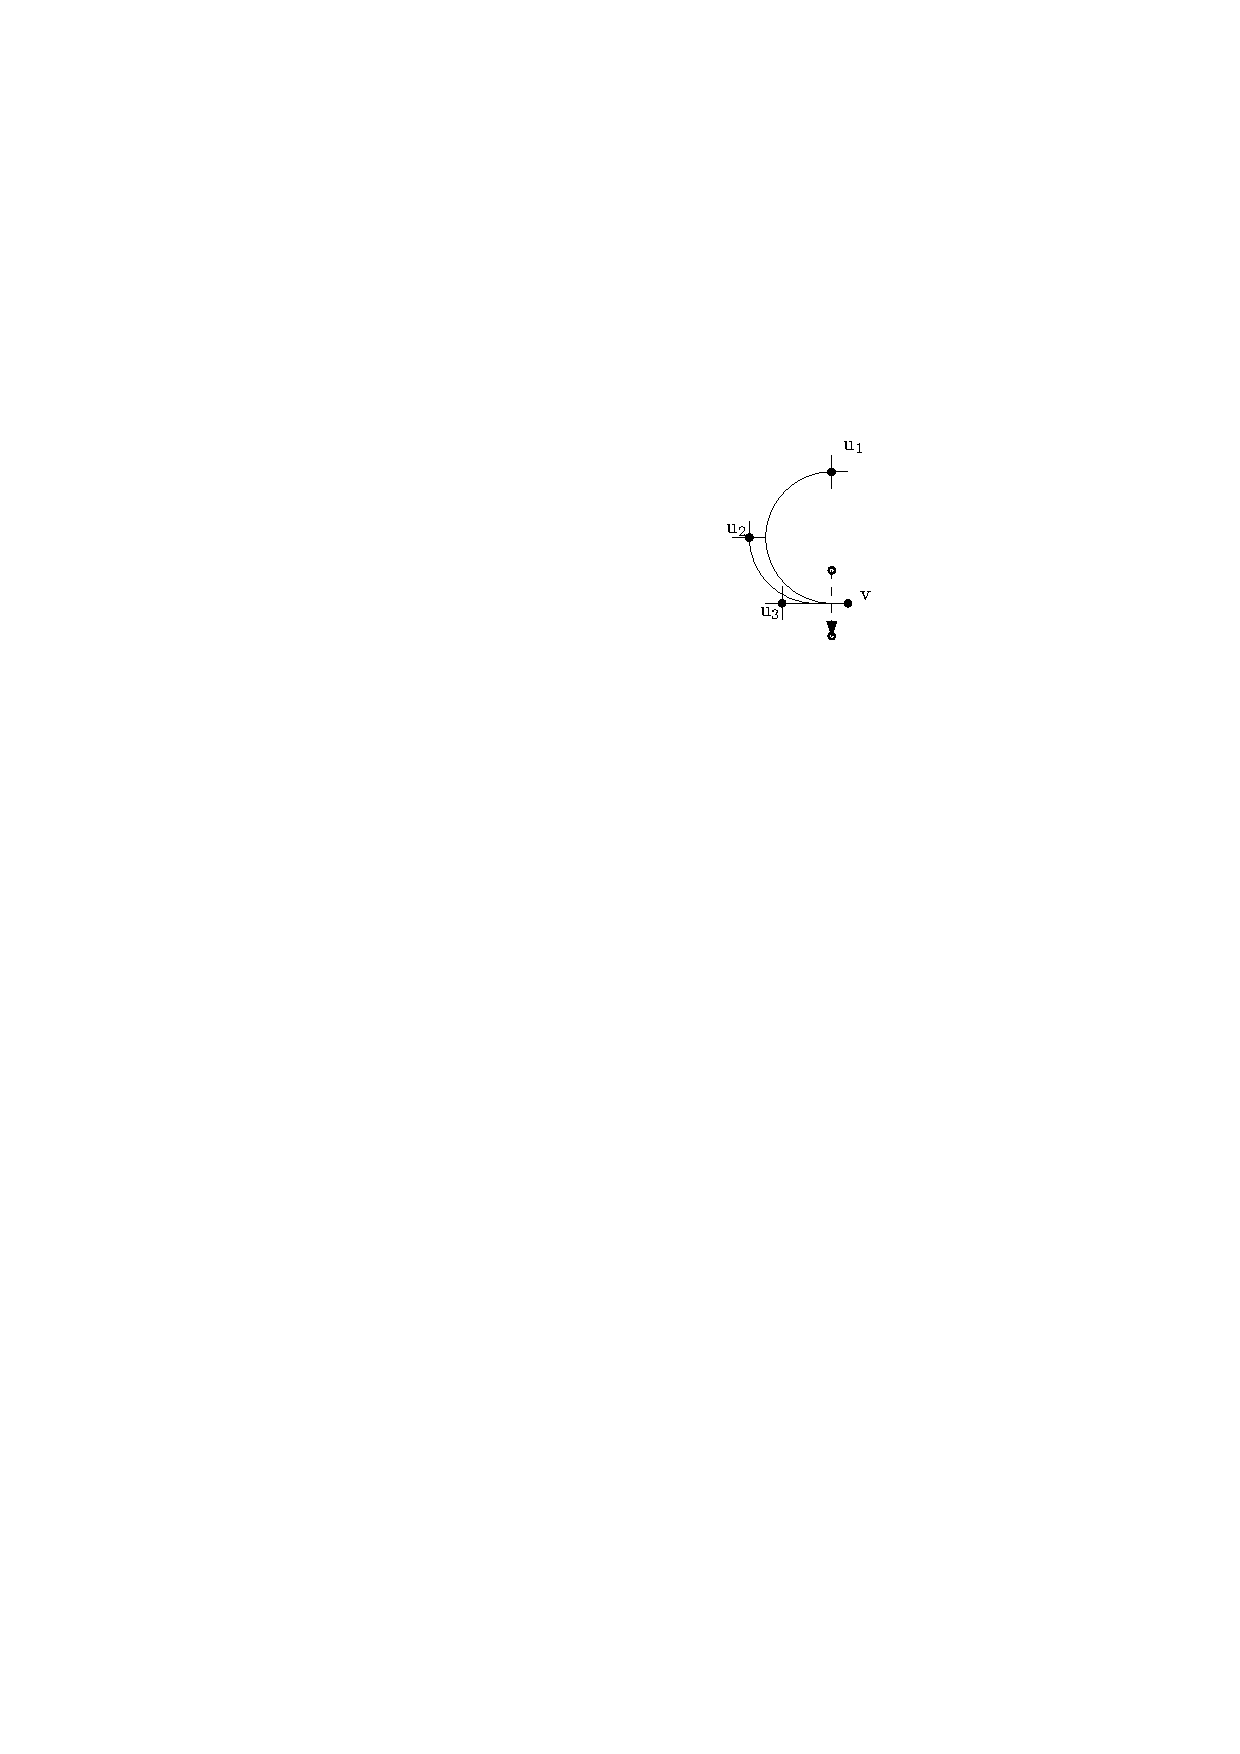
\includegraphics[width=\textwidth]{schnitt_finden/top_upwards}
                \caption{Oberhalb, Kante \\ nach oben}
                \label{fig:cutfinding_top_upwards}
        \end{subfigure}
        \quad
        \begin{subfigure}[b]{0.2\textwidth}
                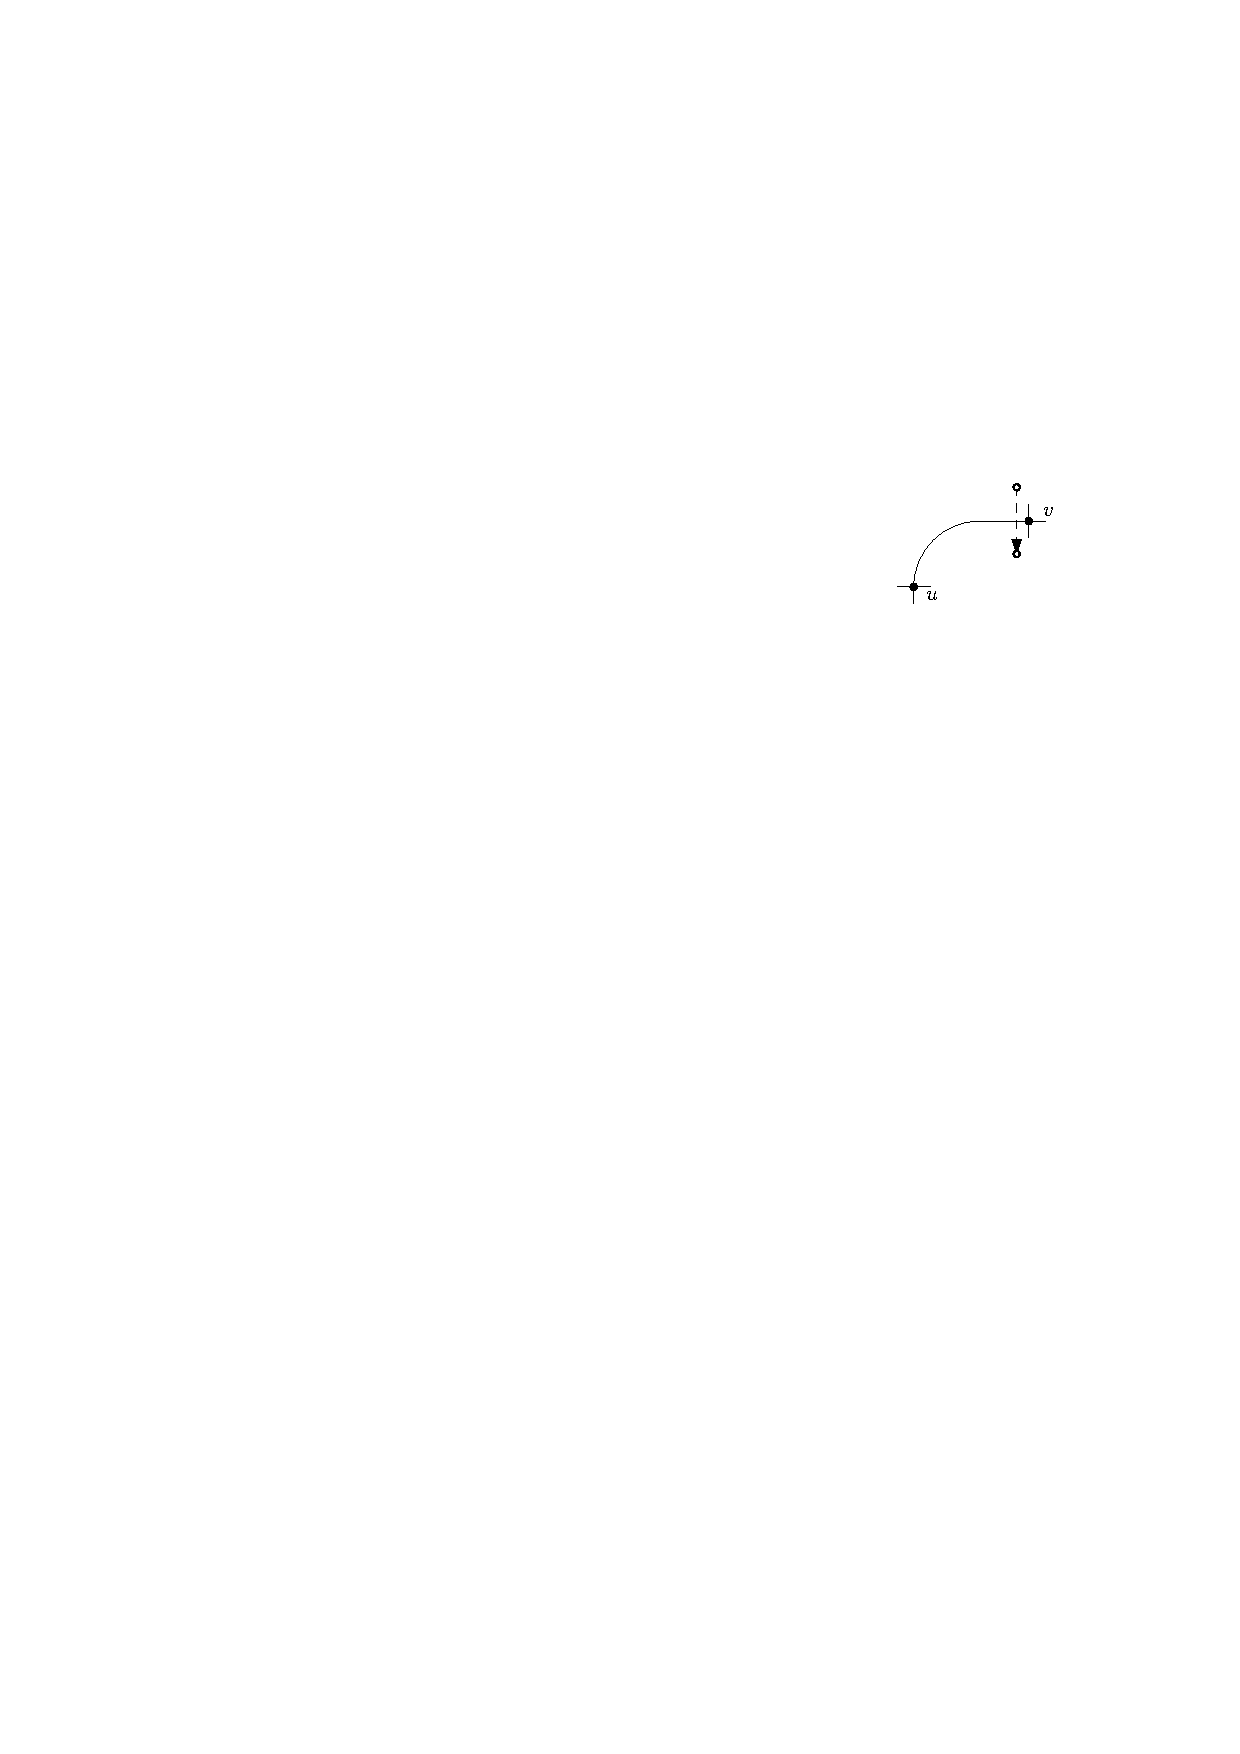
\includegraphics[width=\textwidth]{schnitt_finden/top_downwardsL}
                \caption{Oberhalb, L"~Kante \\ nach unten}
                \label{fig:cutfinding_top_downwardsL}
        \end{subfigure}
        \quad
        \begin{subfigure}[b]{0.2\textwidth}
                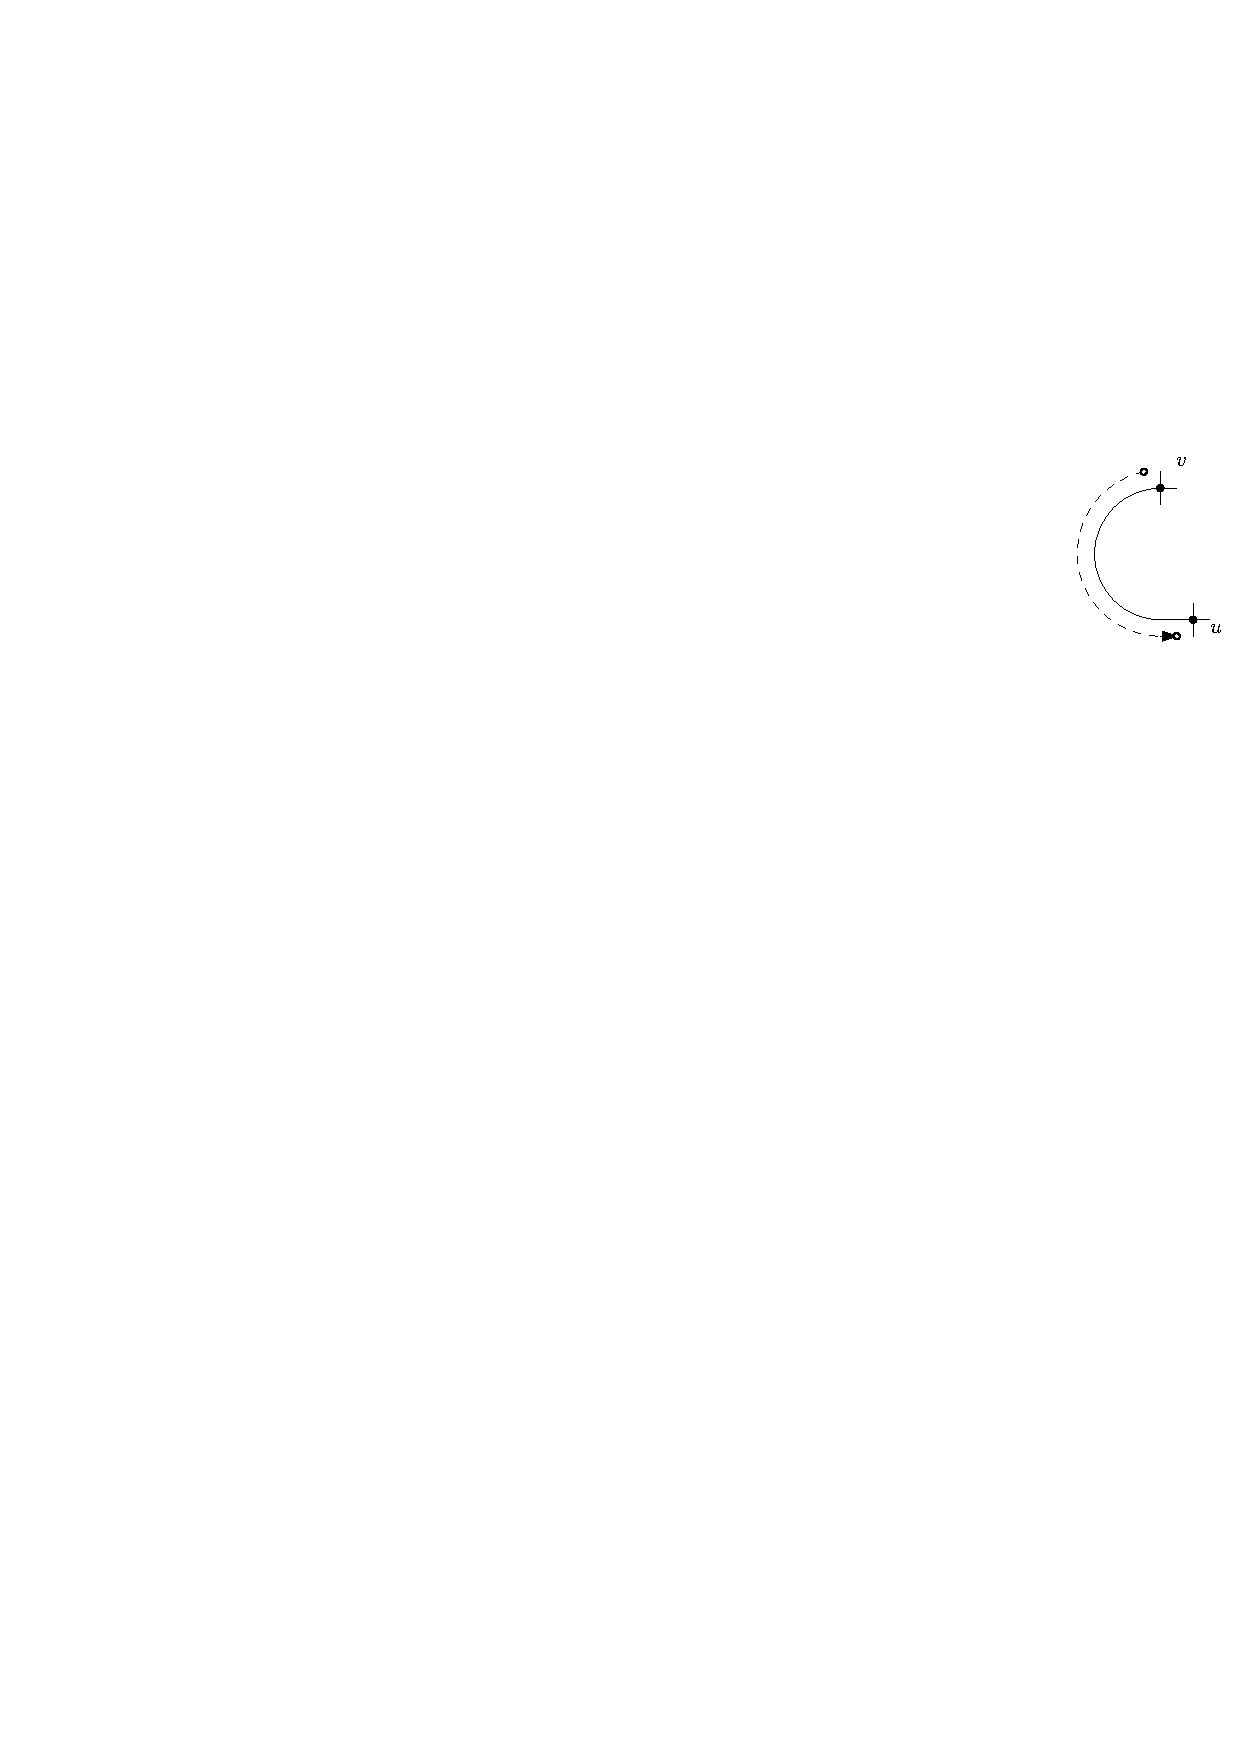
\includegraphics[width=\textwidth]{schnitt_finden/top_downwardsC}
                \caption{Oberhalb, C"~Kante \\ nach unten}
                \label{fig:cutfinding_top_downwardsC}
        \end{subfigure}
        \quad
        \begin{subfigure}[b]{0.2\textwidth}
                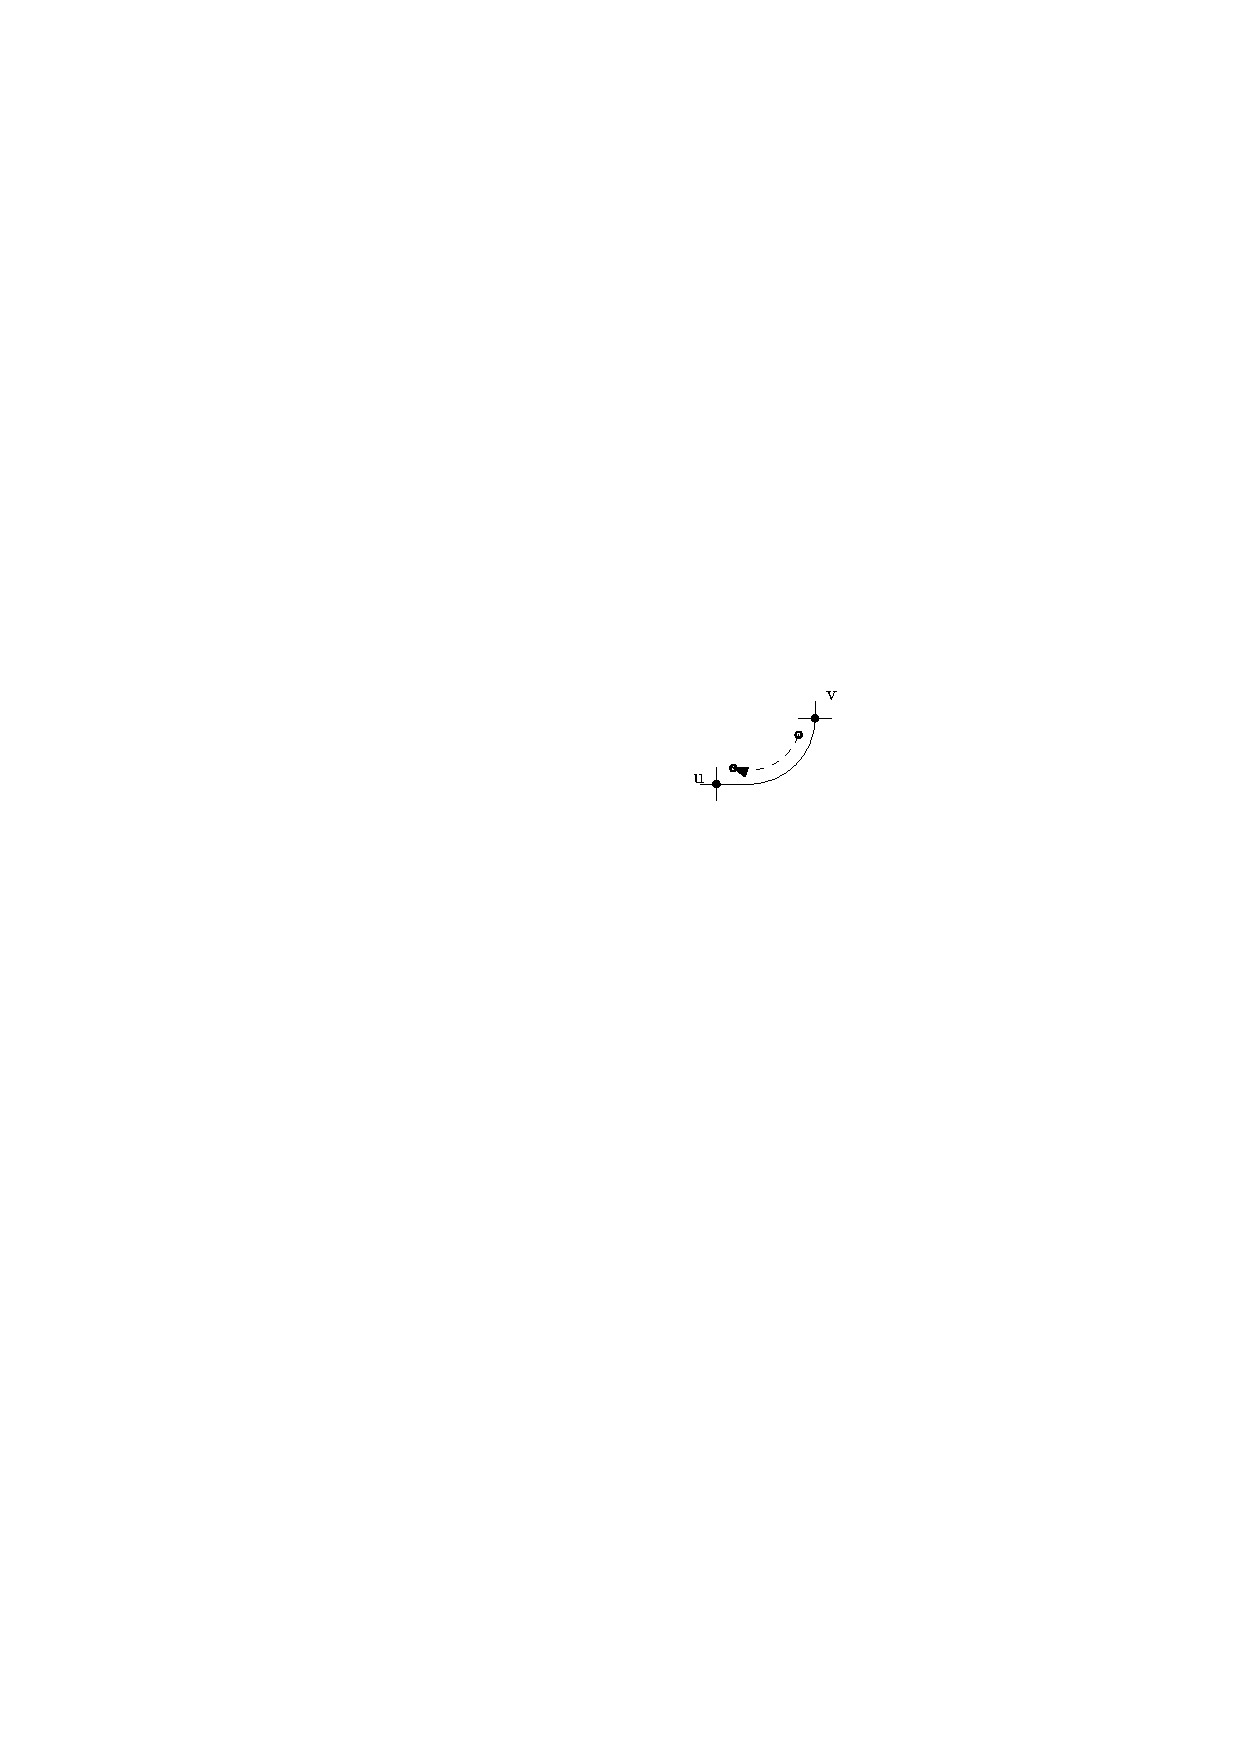
\includegraphics[width=\textwidth]{schnitt_finden/bot_aboveL}
                \caption{Unterhalb, über eine \\ L"~Kante}
                \label{fig:cutfinding_bot_aboveL}
        \end{subfigure}
        \quad
        \begin{subfigure}[b]{0.2\textwidth}
                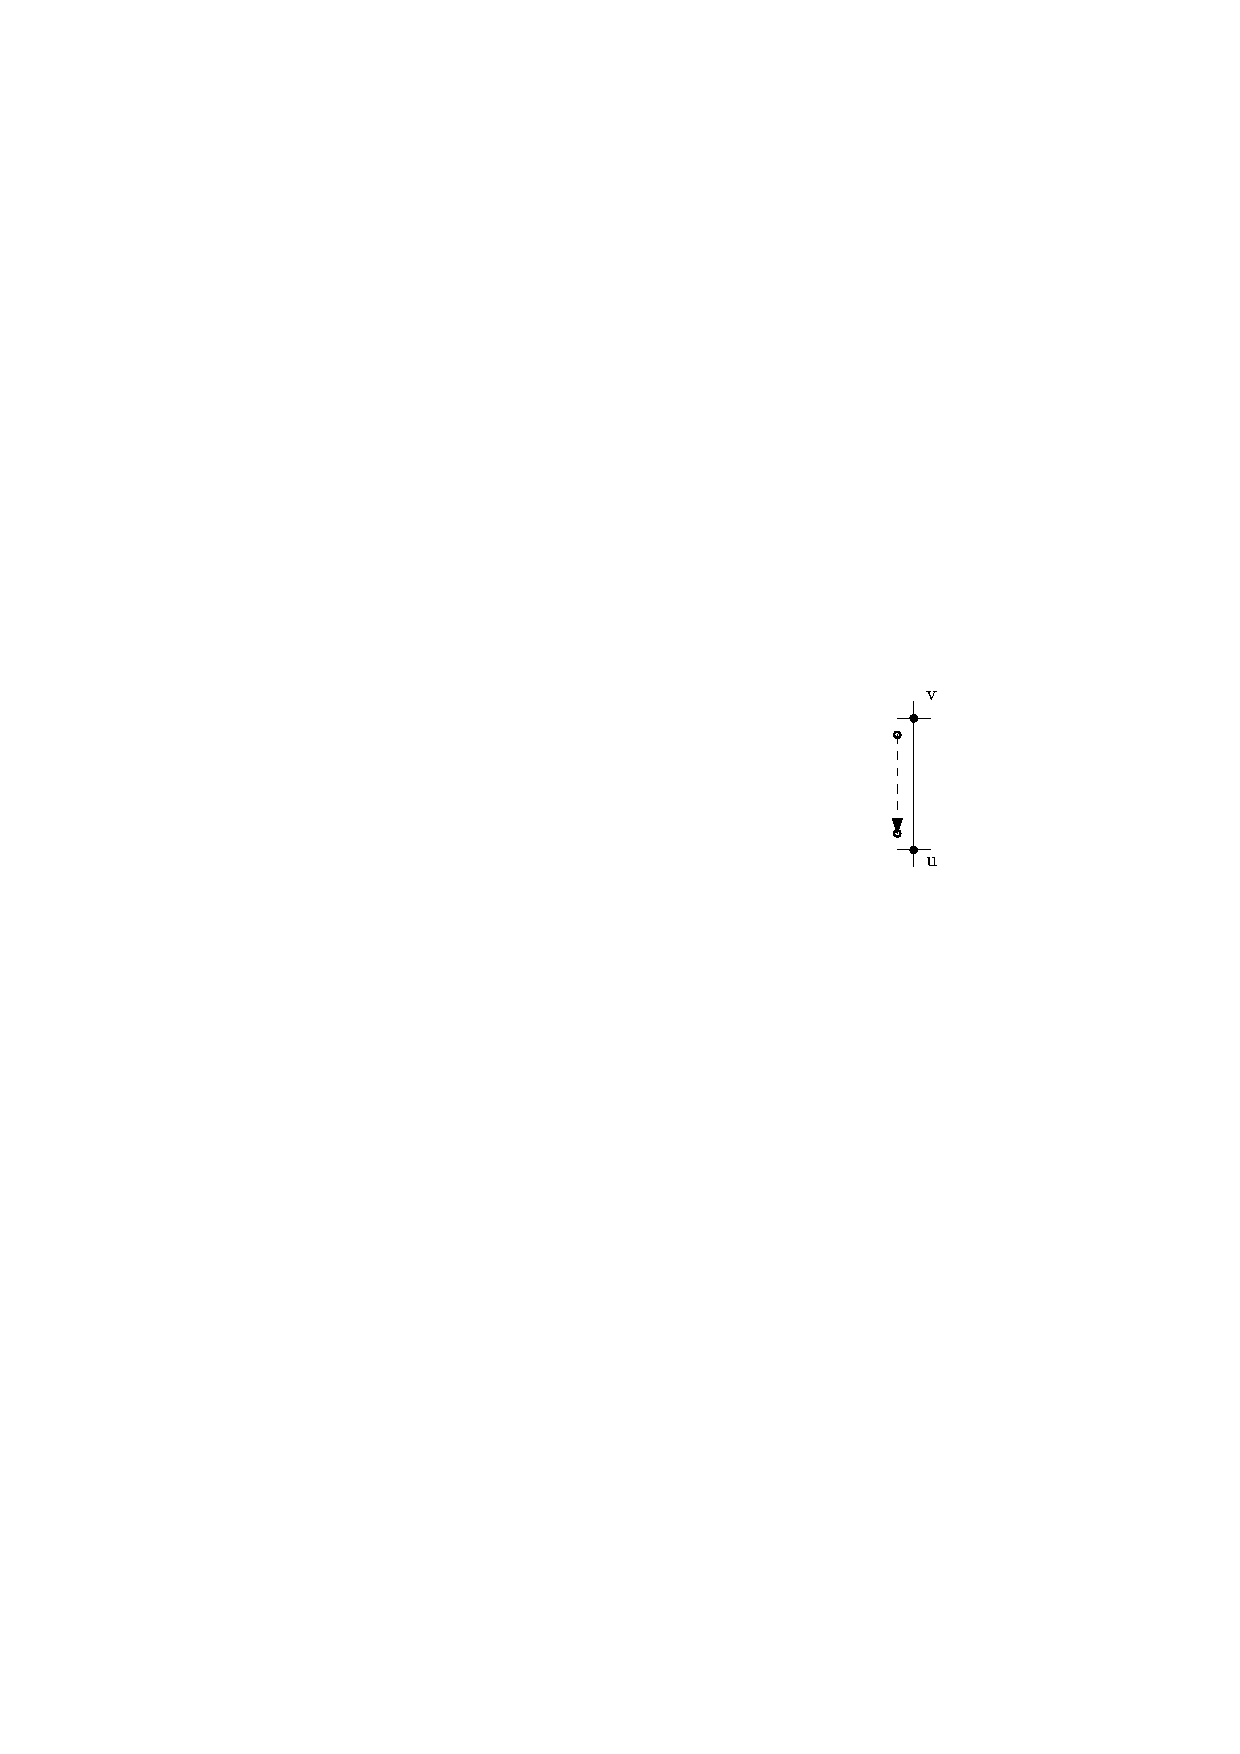
\includegraphics[width=0.25\textwidth]{schnitt_finden/bot_vertical}
                \caption{Unterhalb, entlang einer vertikalen Kante}
                \label{fig:cutfinding_bot_vertical}
        \end{subfigure}
        \quad
        \begin{subfigure}[b]{0.2\textwidth}
                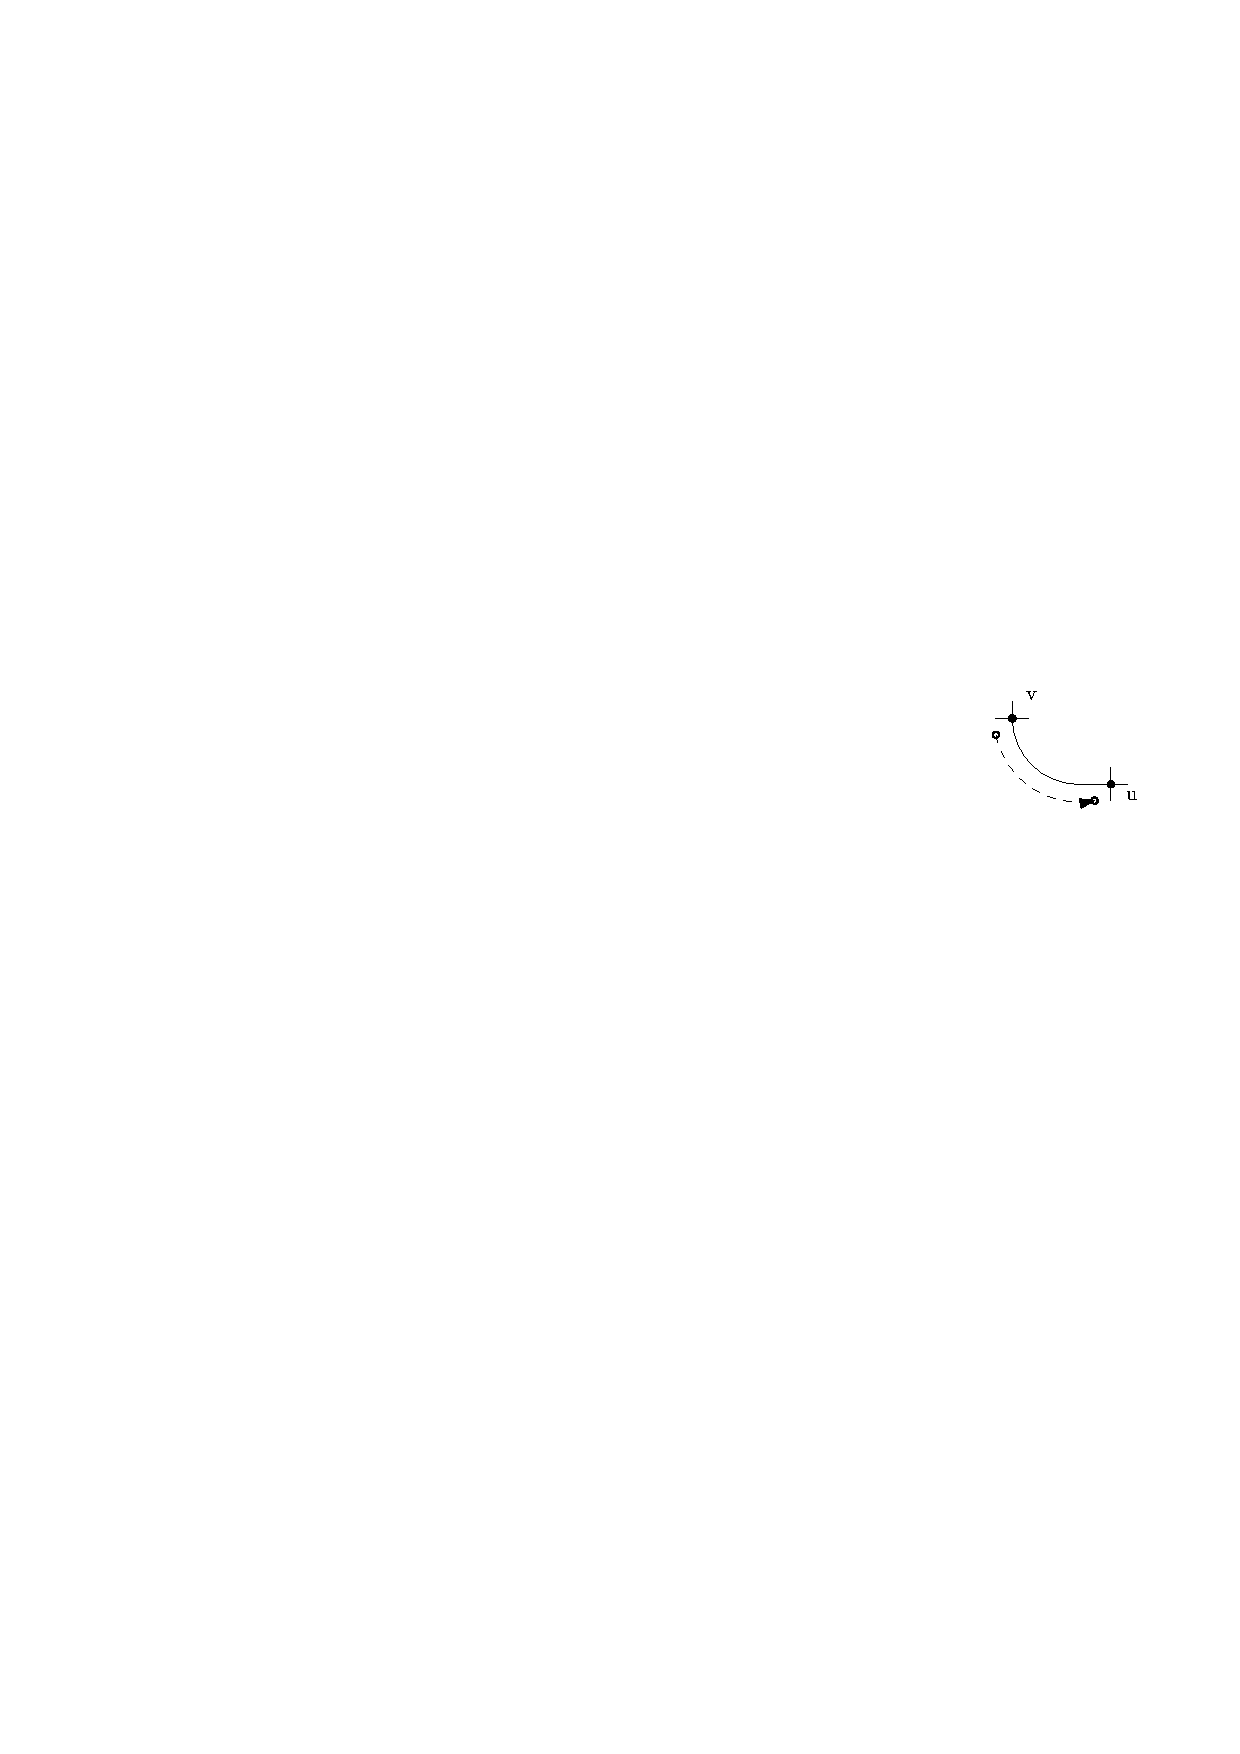
\includegraphics[width=\textwidth]{schnitt_finden/bot_belowL}
                \caption{Unterhalb, \\ unter eine \\ L-Kante}
                \label{fig:cutfinding_bot_belowL}
        \end{subfigure}
        \caption{Die verschiedenen Fälle beim Finden eines Schnitts bei Beginn auf der linken Seite.}\label{fig:cutfinding}
\end{figure}


Soll der Schnitt leicht oberhalb eines Knotens $v$ beginnen, so muss die Kante am linken Port betrachtet werden. Ist dort keine Kante vorhanden, kann der Schnitt direkt zur leicht unterhalb Position am gleichen Knoten $v$ fortfahren. Ist dort eine nach oben führende Kante oder eine horizontale gerade Kante, so durchquert der Schnitt die Kante. Durch die Anpassung der Steigung der L"~Kanten und die Behandlung der C"~Kanten ist immer ein horizontales Segment an dieser Stelle. Der Schnitt verbleibt am Knoten $v$ und ist nun leicht unterhalb von $v$. Führt die Kante am linken Port nach unten, so muss es entweder eine L- oder eine C"~Kante sein, in beiden Fällen folgt der Schnitt der Kante zum Zielknoten $u$. Die L"~Kante endet am Zielknoten $u$ am oberen Port und der Schnitt endet links oberhalb des Zielknotens. Die C"~Kante endet am Zielknoten $u$ am linken Port und der Schnitt endet links unterhalb.

Soll der Schnitt leicht unterhalb eines Knotens $v$ beginnen, so muss die Kante am unteren Port betrachtet werden. Endet die Kante an $u$ an einem rechten Port, so muss sie durchquert werden, und der Schnitt endet leicht rechts unterhalb des Zielknotens $u$. Ansonsten folgt der Schnitt der Kante. Endet die Kante an einem oberen Port, ist folglich eine gerade Kante, so endet der Schnitt leicht links oberhalb des Zielknotens. Endet die Kante an einem linken Port, liegt eine L"~Kante vor und der Schnitt endet leicht links unterhalb des Zielknotens.

Für den Fall, dass der Schnitt leicht rechts eines Knotens beginnt, sind jeweils "`rechts"' und "`links"' in den Schritten und Bedingungen zu tauschen. Nach wiederholter Anwendung dieser Regeln, wobei jeweils der Zielknoten zum neuen Ausgangsknoten wird, gelangt der Schnitt schließlich zur Position leicht unterhalb eines Knotens, der keine Kante am unteren Port hat. Dies ist der unterste Knoten, und der Schnitt ist abgeschlossen.

Die Konstruktion des Schnittes speichert bei jedem Durchqueren einer Kante die Kante selbst, und den Knoten links und rechts der Kante jeweils in einer Liste von linken und rechten Knoten. Zum Finden der gesamten linken Knoten wird an jedem der Knoten in der Liste der linken Knoten eine Tiefensuche begonnen, die jedoch nicht den durchgeschnittenen Kanten folgt. Ebenso findet man die rechten Knoten, indem man bei allen rechten Knoten startet und wiederum durchgeschnittene Kanten ignoriert.

\section{Erkennung von Überschneidungen bei glatt"=orthogonalen Kanten}

Im Verlauf des Algorithmus wird die Fähigkeit benötigt, Überschneidungen zwischen Kanten zu erkennen. Es muss möglich sein, für eine Kante zu prüfen, ob sie mit einer Teilmenge der bereits gezeichneten Kanten Überschneidungen bildet. Außerdem sollte die fertige Zeichnung auf Überschneidungen zwischen zwei beliebigen Kanten geprüft werden können, damit Fehler im Algorithmus erkannt werden können. Hierbei muss die Existenz von Schnittpunkten von Liniensegmenten und Kreissegmenten geprüft werden. Da alle Knoten auf einem ganzzahligen Koordinatengitter sind, die Durchmesser der Kreissegmente ganzzahlig sind, und die Kreissegmente sich nur über vielfache von 90\textdegree~Winkeln beginnend Gitterpunkten erstrecken, ist es möglich, die Kollisionen nur mit Ganzzahlarithmetik zu testen. Daraus wären Vorteile in Genauigkeit und Geschwindigkeit zu erwarten. Wir haben jedoch für die Implementierung auf Verfahren der analytischen Geometrie zurückgegriffen. Damit ist die Lösung flexibler, sie kann auf beliebige Kreis- und Liniensegmente angewendet werden.

% TODO: Mit Formeln etc. genauer beschreiben?

\chapter{Verbesserungen und empirische Untersuchung}
\label{chap:results}

In den vorausgegangenen Kapiteln wurde beschrieben, wie der Algorithmus funktioniert, wie er implementiert wurde. Dabei wurden einige Erkenntnisse aus dem Prozess der Implementierung vorgestellt. Dieses Kapitel soll nun Erkenntnisse vorstellen, die auf Grundlage der Implementierung über den Algorithmus gewonnen wurden: Die Implementierung erlaubt es, den Algorithmus automatisiert auf eine Vielzahl von Graphen anzuwenden. Die gewonnenen Zeichnungen können mit bestimmten Metriken in ihrer Qualität beurteilt werden.

\section{Bewertungskriterien für glatt"=orthogonale Zeichnungen}

Die Zeichnungen wurden nach verschiedenen Kriterien bewertet. Für jedes dieser Kriterien wird nun erklärt, was es bedeutet, wie es erhoben wurde, und warum genau dieses Kriterium ausgewählt wurde.

Ein Kriterium ist die verbrauchte \emph{Fläche}: Visualisierungen von Graphen können in ihrer Qualität eingestuft werden, je nachdem, wie viel Platz sie verbrauchen. Nun sind die Zeichnungen natürlich skalierbar, informell ausgedrückt: Ein Bild kann größer oder kleiner ausgedruckt werden. Deshalb misst man die Größe bei einer konstanten Auflösung. Für allgemeine Zeichnungen kann der kleinste Abstand zwischen zwei Knoten als Referenz gewählt werden: Werden alle Zeichnungen auf dieselbe Ausgabefläche skaliert, so schneidet eine Zeichnung, die im Vergleich zu diesem Mindestabstand viel Platz verbraucht, schlecht ab, da die beiden nahen Knoten kaum noch unterscheidbar sind. Benötigt eine Zeichnung jedoch wenig Fläche, so können die Knoten klar voneinander unterschieden werden.

Für orthogonale und glatt"=orthogonale Zeichnungen ist die kürzeste mögliche Entfernung zwischen zwei Knoten der Abstand zweier Gitterlinien. Somit wird die Fläche in Gitterabständen gemessen. Da orthogonale und glatt"=orthogonale Zeichnungen üblicherweise auf einer rechteckigen Fläche gezeichnet werden, wird die die Fläche einer Zeichnung als das Produkt der Seitenlängen eines minimalen umgebenden Rechtecks (englisch \emph{bounding box}) aller Knoten und Kanten festgelegt.

Ein weiteres Kriterium ist die \emph{Fläche pro Knoten}: Auf einer ein Gitterquadrat großen Fläche lassen sich maximal vier Knoten platzieren. Somit sagt der Quotient von Fläche und Knotenanzahl auch etwas über die Effektivität der Darstellung aus.

Da Liu et al.~\cite{liu+etal-98} die obere Grenze für die Fläche der OC$_3$-Zeichnungen mit $(|V|+1)^2$ angeben, soll auch untersucht werden, ob im Durchschnittsfall mit einer quadratischen Flächenzunahme zu rechnen ist. Ein Graph mit 18~Knoten hätte also im schlechtesten Fall eine Fläche von 361 Gitterquadraten, also 20 je Knoten.

Eine minimale Fläche pro Knoten lässt sich nicht angeben: Eine Zeichnung eines Pfades, bei der alle Knoten auf einer Linie liegen hätte keine definierte Breite und somit die Fläche~0. Betrachtet man ein Quadrat der Seitenlänge $l$~Gittereinheiten und der Fläche $A = l^2$, so passen in das Quadrat horizontal und vertikal je $l+1$ Gitterlinien. Somit kann es $|V|_\text{max} = (l + 1)^2$ Knoten fassen, wenn diese jeweils auf den Gitterkreuzen positioniert werden. Sollen umgekehrt $|V|$ Knoten in einem Quadrat positioniert werden, so muss seine Fläche mindestens $A = (\lceil\sqrt{|V|}\rceil - 1)^2$ betragen. Für sehr große Quadrate ergibt sich also eine Fläche von $(\lceil\sqrt{|V|}\rceil - 1)^2 /|V| \approx \sqrt{|V|}^2 / |V|  = 1$ Gitterquadrat pro Knoten. 

Das dritte Kriterium ist die \emph{Segmentzahl}: Es können zwar bei SC$_2$-Zeichnungen nur maximal zwei Segmente pro Kante vorliegen, doch oftmals ist es möglich, das Layout so anzupassen, dass eine Kante mit nur einem Segment gezeichnet wird.  Jedoch wird in \cite{bekos-13} gezeigt, dass der Flächenzuwachs bei einer Konversion in ein SC$_1$-Layout exponentiell sein kann. Zeichnungen mit exponentieller Fläche sind nicht praxistauglich, und somit ist eine niedrigere Segmentzahl nicht wünschenswert, wenn sie gleichzeitig mit hohem Flächenzuwachs verbunden ist.

\section{Erhobene Messwerte}

Als Vergleichsgraphen für das Erstellen von Zeichnungen wurden die Rom-Testgraphen verwendet. Nachdem einige Graphen entfernt wurden, z.B.\ weil sie nicht zweifach zusammenhängend sind, blieb eine Menge von 844~Graphen, die jeweils mit den verschiedenen Methoden gezeichnet wurden. Die Graphen enthalten zwischen 10 und 51~Knoten, in Abbildung~\ref{fig:graphSizes} erkennt man, wie viele Graphen mit welchen Knotenanzahlen verarbeitet wurden. Der Großteil der Graphen (73\%) hat zwischen elf und zwanzig Knoten, bei durchschnittlich 18,2~Knoten. Würden alle diese Graphen die maximale Fläche von $(|V|+1)^2$ benötigen, ergäben sich im Mittel durchschnittlich 20,25 Gitterquadraten je Knoten.

Für die OC$_3$-Zeichnungen lag die durchschnittliche Fläche pro Knoten im Mittel bei 4,768 Gitterquadraten. In Abbildung~\ref{fig:ortho-noCompress} wird die Verteilung von Knotenanzahlen und Fläche gezeigt. Das Diagramm liegt in doppelt logarithmischer Darstellung vor. Das bedeutet, ein Polynom der Form $A = a|V|^b$ wird zu einer Gerade $y = \log{a} + bx$. Als Referenz wurden in grau die Geraden für die Formeln $(|V|+1)^2$ des theoretischen Flächenmaximums oben und $(\sqrt{|V|}+1)^2$ für die perfekte Platzierung in einem Quadrat unten eingefügt. Einige Zeichnungen liegen unterhalb dieser Grenze, das liegt daran, dass sie nicht quadratisch sind und somit die Konten effektiver platzieren können. Die diskreten Werte für die Knotenanzahl wurden mit einem leichten Rauschen versehen, sodass nicht alle Kreuze auf einer Linie liegen, sondern eine Wolke bilden und die Dichte der Messpunkte besser zu erkennen ist. 

Die Fläche aller Graphen bleibt stets deutlich unter dem theoretischen Maximum zurück. Es besteht eine Korrelation zwischen Knotenanzahl und Flächenbedarf: Die Steigung der Punktewolke entspricht etwa der der oberen Grenze, weshalb angenommen werden kann, dass der Flächenbedarf im Mittel quadratisch mit der Knotenzahl zunimmt und um einen konstanten Faktor kleiner ist, als das theoretische Maximum. Es gibt keine extremen Ausreißer. Dass sich hier auch für die Fläche so wenige diskrete Werte ergeben, liegt daran, dass die Höhe $h$ der Zeichnungen direkt mit der Knotenanzahl zusammenhängt, sie liegt im Bereich $|V| \leq h \leq |V| + 2$.

Nach der Komprimierung und der Entfernung der stufenförmigen Kanten konnte die mittlere Fläche pro Knoten auf durchschnittlich 3,526 Gitterquadrate gesenkt werden. In Abbildung~\ref{fig:ortho-compress} wird die Verteilung von Knotenanzahlen und Fläche gezeigt, wenn die Nachbearbeitung verwendet wird. Der Flächenbedarf ist nochmals um einen Faktor  geringer und die Zahl der diskreten Flächenwerte ist größer. Ansonsten ergibt sich ein ähnliches Bild.

Für die glatt"=orthogonalen Zeichnungen ergab sich durchschnittlich eine Fläche von 16,94 Gitterquadraten pro Knoten. Abbildung~\ref{fig:smooth-noOpti} zeigt auch hier die Verteilung. Die 18\,713 Kanten aller Zeichnungen hatten durchschnittlich 1,1934 Segmente, viele Kanten haben also nur Komplexität~1. Der Flächenbedarf ist größer, die Streuung ist hoch und es gibt oftmals Ausreißer nach oben. Der Punkt beim x"~Wert 40~Knoten mit dem größten Flächenbedarf ist die Zeichnung aus Abbildung~\ref{fig:smoothBadnessShowing}. Hier sorgt das Verschieben eines Plateaus nach oben, um Kollisionen im Inneren einer C"~Kante zu verhindern, wie in Abbildung~\ref{fig:accomodateCedge} für eine enorme Höhe. Die Knoten sind teilweise sehr nah und in der Gesamtansicht kaum zu unterscheiden und es gibt große, leere Flächen, die Verteilung der Knoten ist unausgewogen. Insgesamt ergibt sich ein Bild der Unzuverlässigkeit: In vielen Fällen ist der Flächenbedarf nur etwas höher, doch bei einigen Konstellationen wird der Flächenbedarf unpraktikabel hoch.

Das Zeichnen der 844 Testgraphen dauerte auf einem aktuellen handelsüblichen Consumer"=PC rund zehn Sekunden. Die Implementierung wurde nicht weiter auf Geschwindigkeit optimiert, denn diese Bearbeitungsgeschwindigkeit ist bereits für die meisten Anwendungen ausreichend. Es zeigt sich, dass die Implementierung keine schwerwiegenden Probleme mit der Laufzeit hat.

Da der Flächenbedarf für die glatt"=orthogonalen Zeichnungen so stark gestiegen ist, und in einigen Fällen deutlich über das Maximum für orthogonale Zeichnungen $(|V|+1)^2$ hinaus ragt, stellt sich nun die Frage, wie der Flächenbedarf der glatt"=orthogonalen Zeichnungen weiter reduziert werden kann.

\section{Korrektur der Steigung aussetzen}

Eine implementierte Verbesserung setzt bei der Konversion vom OC$_3$- in das SC$_2$-Layout an. Während der Implementierung fiel auf, dass von den 844 OC$_3$-Layouts der Graphen 734 ohne jegliche Anpassung der Knotenpositionen ein planares SC$_2$-Layout darstellen. Hier muss also überhaupt keine Anpassung vorgenommen werden. Ein Beispiel für einen solchen zeigt Abbildung~\ref{fig:smoothOkness}.

Bei den übrigen 110 Graphen wurden daraufhin alle Anpassungen vorgenommen, bis auf solche, die nur zur Korrektur der Steigung der L"~Kanten verwendet werden. Wird also ein Knoten platziert, dann erfolgen die Anpassungen, die nötig sind, dass seine eingehenden Kanten planar gezeichnet werden. Ist also beispielsweise eine eingehende L"~Kante an seinem linken Port und Teile der Zeichnung ragen von rechts in die Kante hinein, so wird der untere Knoten der Kante wie gehabt nach links verschoben, bis die Kante ohne Überschneidungen gezeichnet werden kann. Normalerweise würde der Algorithmus daraufhin die Steigung der Kante prüfen und, wenn die Kante steiler als 45\textdegree\ absteht, den unteren Knoten noch weiter nach links verschieben, wie bereits in Abbildung~\ref{fig:cutLslopecorrection} gesehen. Auf diese Anpassung wird nun verzichtet. 

Man erinnere sich, dass die Anpassung der Steigung erfolgte, damit die L"~Kante ein horizontales Segment besitzt. Nun besitzt sie mitunter kein horizontales Segment, dafür jedoch ein vertikales. Damit keine Einschränkung in der Fähigkeit Schnitte zu finden entsteht, erlauben wir einen Schnitt durch die L"~Kante, ganz so, also ob dort ein horizontales Segment bestünde. Wenn nun ein solcher Schnitt erfolgt und die Kante in der Folge breiter gezogen wird, kann nicht einfach nur ihr horizontales Segment verlängert werden. Stattdessen wird ihr Kreissegment größer und das vertikale Liniensegment verkürzt. Dabei kann es zu neuen Überschneidungen kommen. Erst wenn die Kante so weit auseinandergezogen wurde, dass die Steigung kleiner als 45\textdegree\ ist, verschwindet das vertikale Liniensegment und es wird bei weiterem Strecken das nun entstandene horizontale Liniensegment verlängert. Wenn alle Knoten platziert sind, wird die erstellte Zeichnung auf Überschneidungen geprüft. Sollte es Überschneidungen geben, wird der Graph erneut mit Anpassung der Steigungen gezeichnet.

Obwohl die Vermutung nahe liegt, dass durch dieses rücksichtslose Vorgehen oftmals neue Überschneidungen entstehen, hat sich dies in der Praxis widerlegt. Von den 110 so angepassten Layouts hatte nur eines danach noch eine Überschneidung. Hier wurde eine L"~Kante auseinandergezogen und bildete neue Überschneidungen, es musste auf den ursprünglichen Algorithmus zurückgegriffen werden. Der Graph in Abbildung~\ref{fig:smoothBadness} konnte mit deutlich geringerem Flächenbedarf gezeichnet werden.

Mit dieser schrittweisen Anpassung der Planaritäts-Maßnahmen konnte die mittlere Fläche pro Konten auf durchschnittlich 7,522 Gitterquadrate gesenkt werden. Abbildung~\ref{fig:smooth-opti} zeigt die Verteilung des Flächenbedarfs je nach Knotenanzahl nach dieser Anpassung. Die Farben der Kreuze für die Zeichnungen kodieren hier, welche Anpassungen vorgenommen wurden. Daran lässt sich erkennen, das über alle Knotenanzahlen hinweg Graphen ohne Anpassungen gezeichnet werden können. Der Flächenbedarf ist auf ein akzeptables Maß gesunken, viele der Ausreißer verschwunden. Es zeichnet sich weiterhin ein quadratisches Wachstum der Fläche ab. Die durchschnittliche Segmentanzahl pro Kante stieg nur leicht auf 1,2189. Abbildung~\ref{fig:areaComparison} zeigt einen zusammenfassenden Vergleich des Flächenbedarfs der verschiedenen Zeichenmethoden.

% --> use them to reduce edge complexity?

% TODO

%%%%%%%
%Verbesserung B
% sets auf gleicher höhe
% keinmal mehr als 3 in einer Reihe
% spezialfall mit 1 in Reihe,

%% spezialfall C-reihenfolge, nur 5 graphen

%%%%%

% Problem mit unnötiger C-Anpasung

%% G-Kanten mit 5 Segmenten

\begin{figure}[h]
  \centering
  {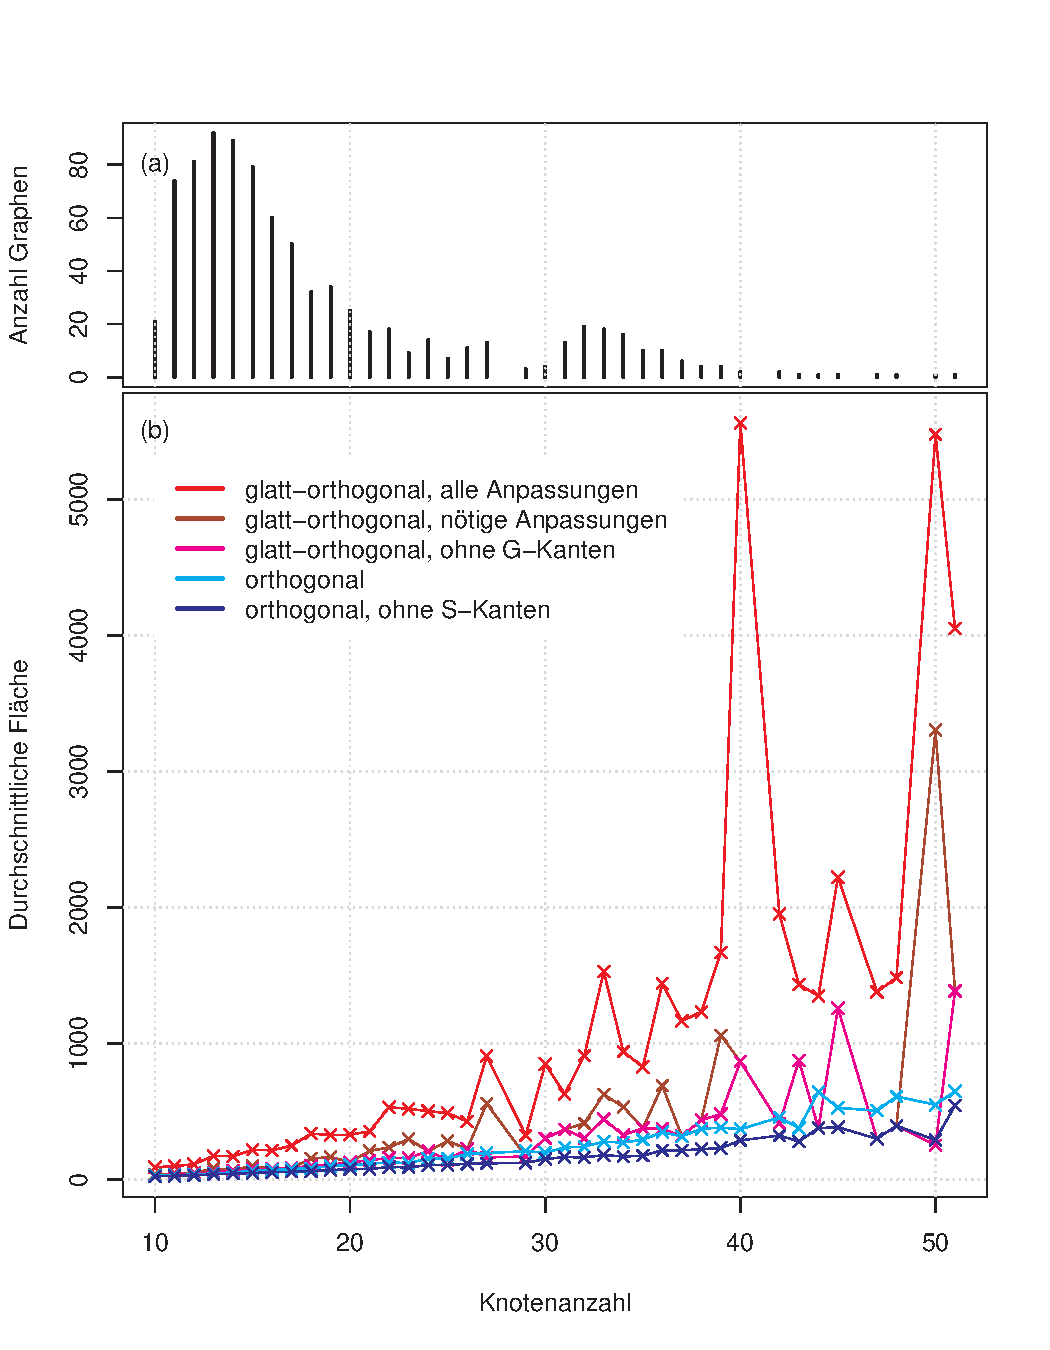
\includegraphics[width=\textwidth]{plots/area_comparison} \phantomsubcaption\label{fig:graphSizes} \phantomsubcaption\label{fig:areaComparison}}
  \caption{Vergleich des durchschnittlichen Flächenbedarfs in Gitterquadraten der verschiedenen Algorithmen nach Anzahl Knoten im Graphen (\subref{fig:areaComparison}) sowie  Verteilung der Anzahl Knoten in den Graphen (\subref{fig:graphSizes}). Zum Vergleich: Eine DIN-A4-Seite von handelsüblichem kariertem Papier hat rund 2400 Gitterquadrate.}
  \label{fig:areaComparisonAndGraphSizes}
\end{figure}
\begin{figure}[h]
  \centering
  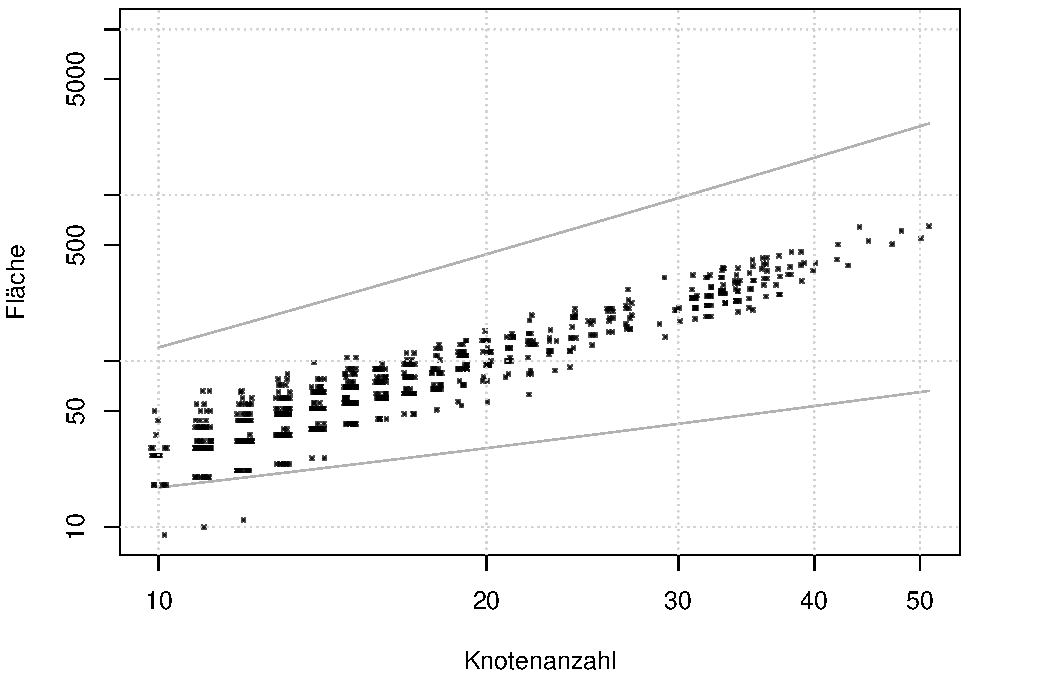
\includegraphics[width=.9\textwidth]{plots/area_orthogonal}
  \caption{Streudiagramm der Fläche der Zeichnungen je nach Knotenanzahl für OC$_3$-Zeichnungen. }
  \label{fig:ortho-noCompress}
\end{figure}
\begin{figure}[h]
  \centering
  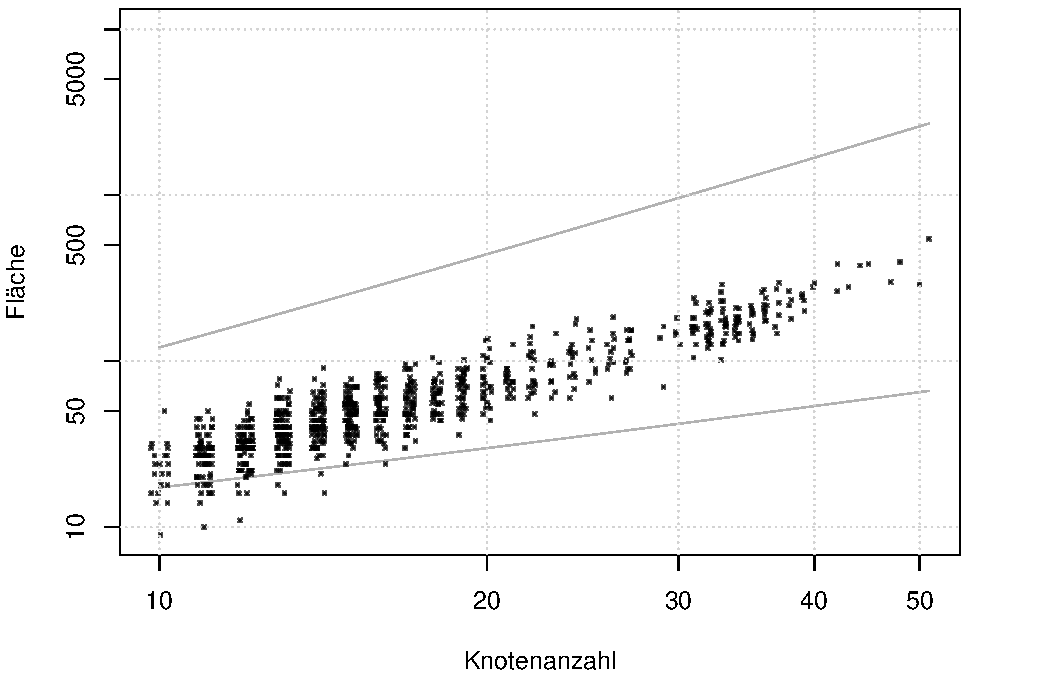
\includegraphics[width=.9\textwidth]{plots/area_orthogonal_compressed}
  \caption{Streudiagramm der Fläche der Zeichnungen je nach Knotenanzahl für OC$_3$-Zeichnungen nach dem Kompressionsschritt ohne stufenförmige Kanten.}
  \label{fig:ortho-compress}
\end{figure}
\begin{figure}[h]
  \centering
  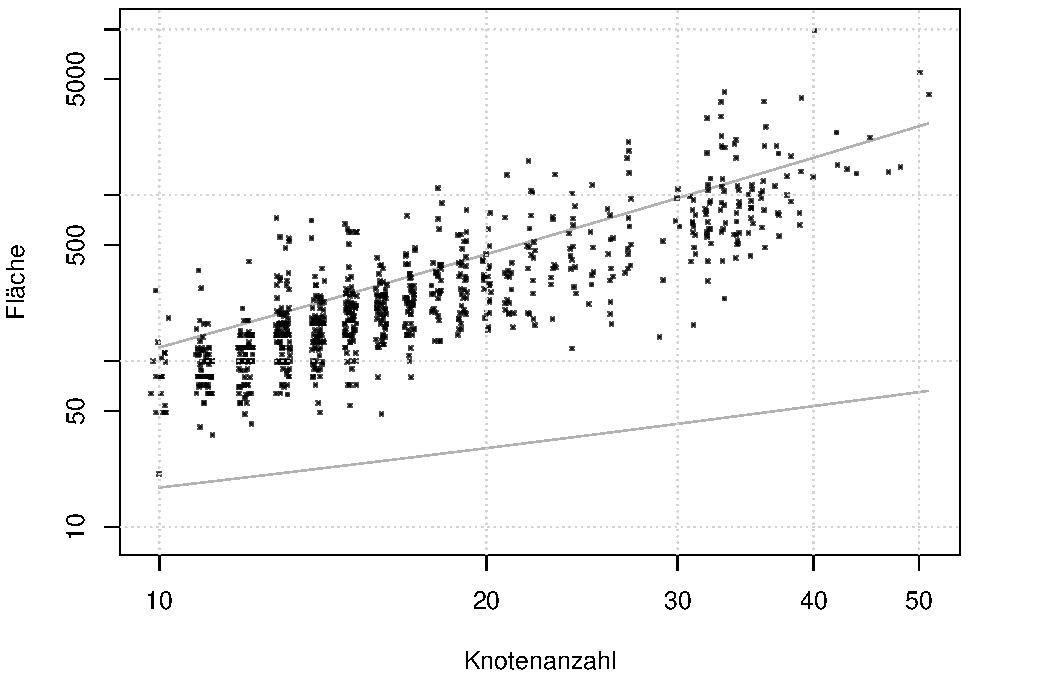
\includegraphics[width=.9\textwidth]{plots/area_smooth}
  \caption{Streudiagramm der Fläche der Zeichnungen je nach Knotenanzahl für SC$_2$-Zeichnungen, wenn die Steigung aller L"~Kanten berichtigt wurde.}
  \label{fig:smooth-noOpti}
\end{figure}
\begin{figure}[h]
  \centering
  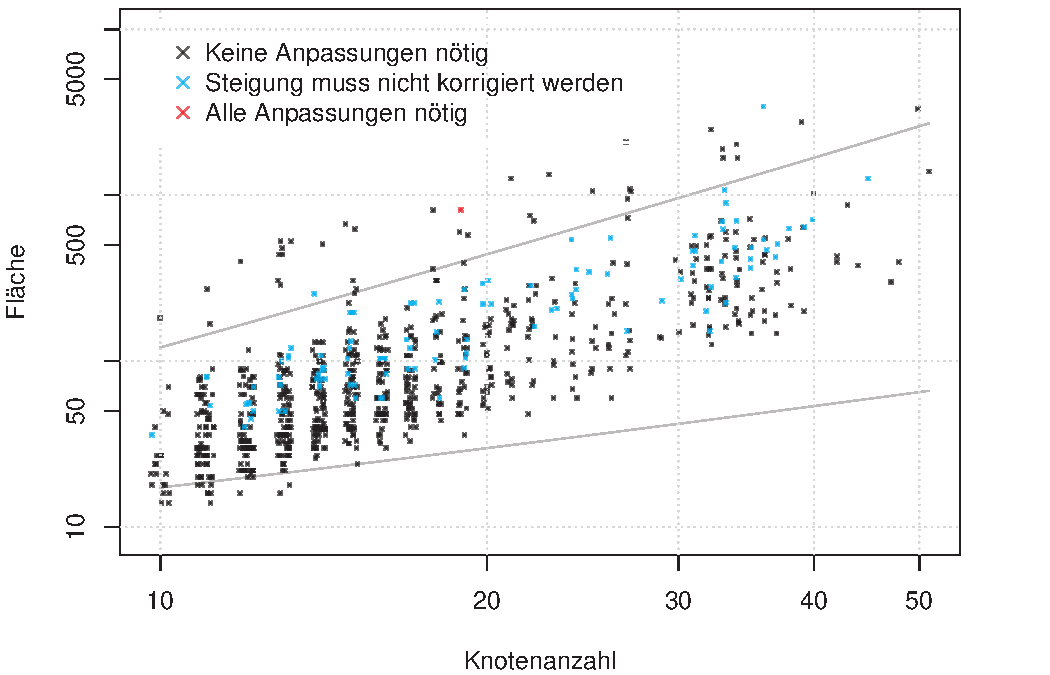
\includegraphics[width=.9\textwidth]{plots/area_smooth_bst}
  \caption{Streudiagramm der Fläche der Zeichnungen je nach Knotenanzahl für SC$_2$-Zeichnungen, wenn die Steigung der L"~Kanten nur bei Bedarf berichtigt wurde.}
  \label{fig:smooth-opti}
\end{figure}

% this is grafo120
\begin{figure}[h]
        \centering
       \subcaptionbox{Gänzlich ohne Korrektur, eine Kante bildet Überschneidungen.\label{fig:smoothBadnessUncorrected}}[0.4\textwidth]
            {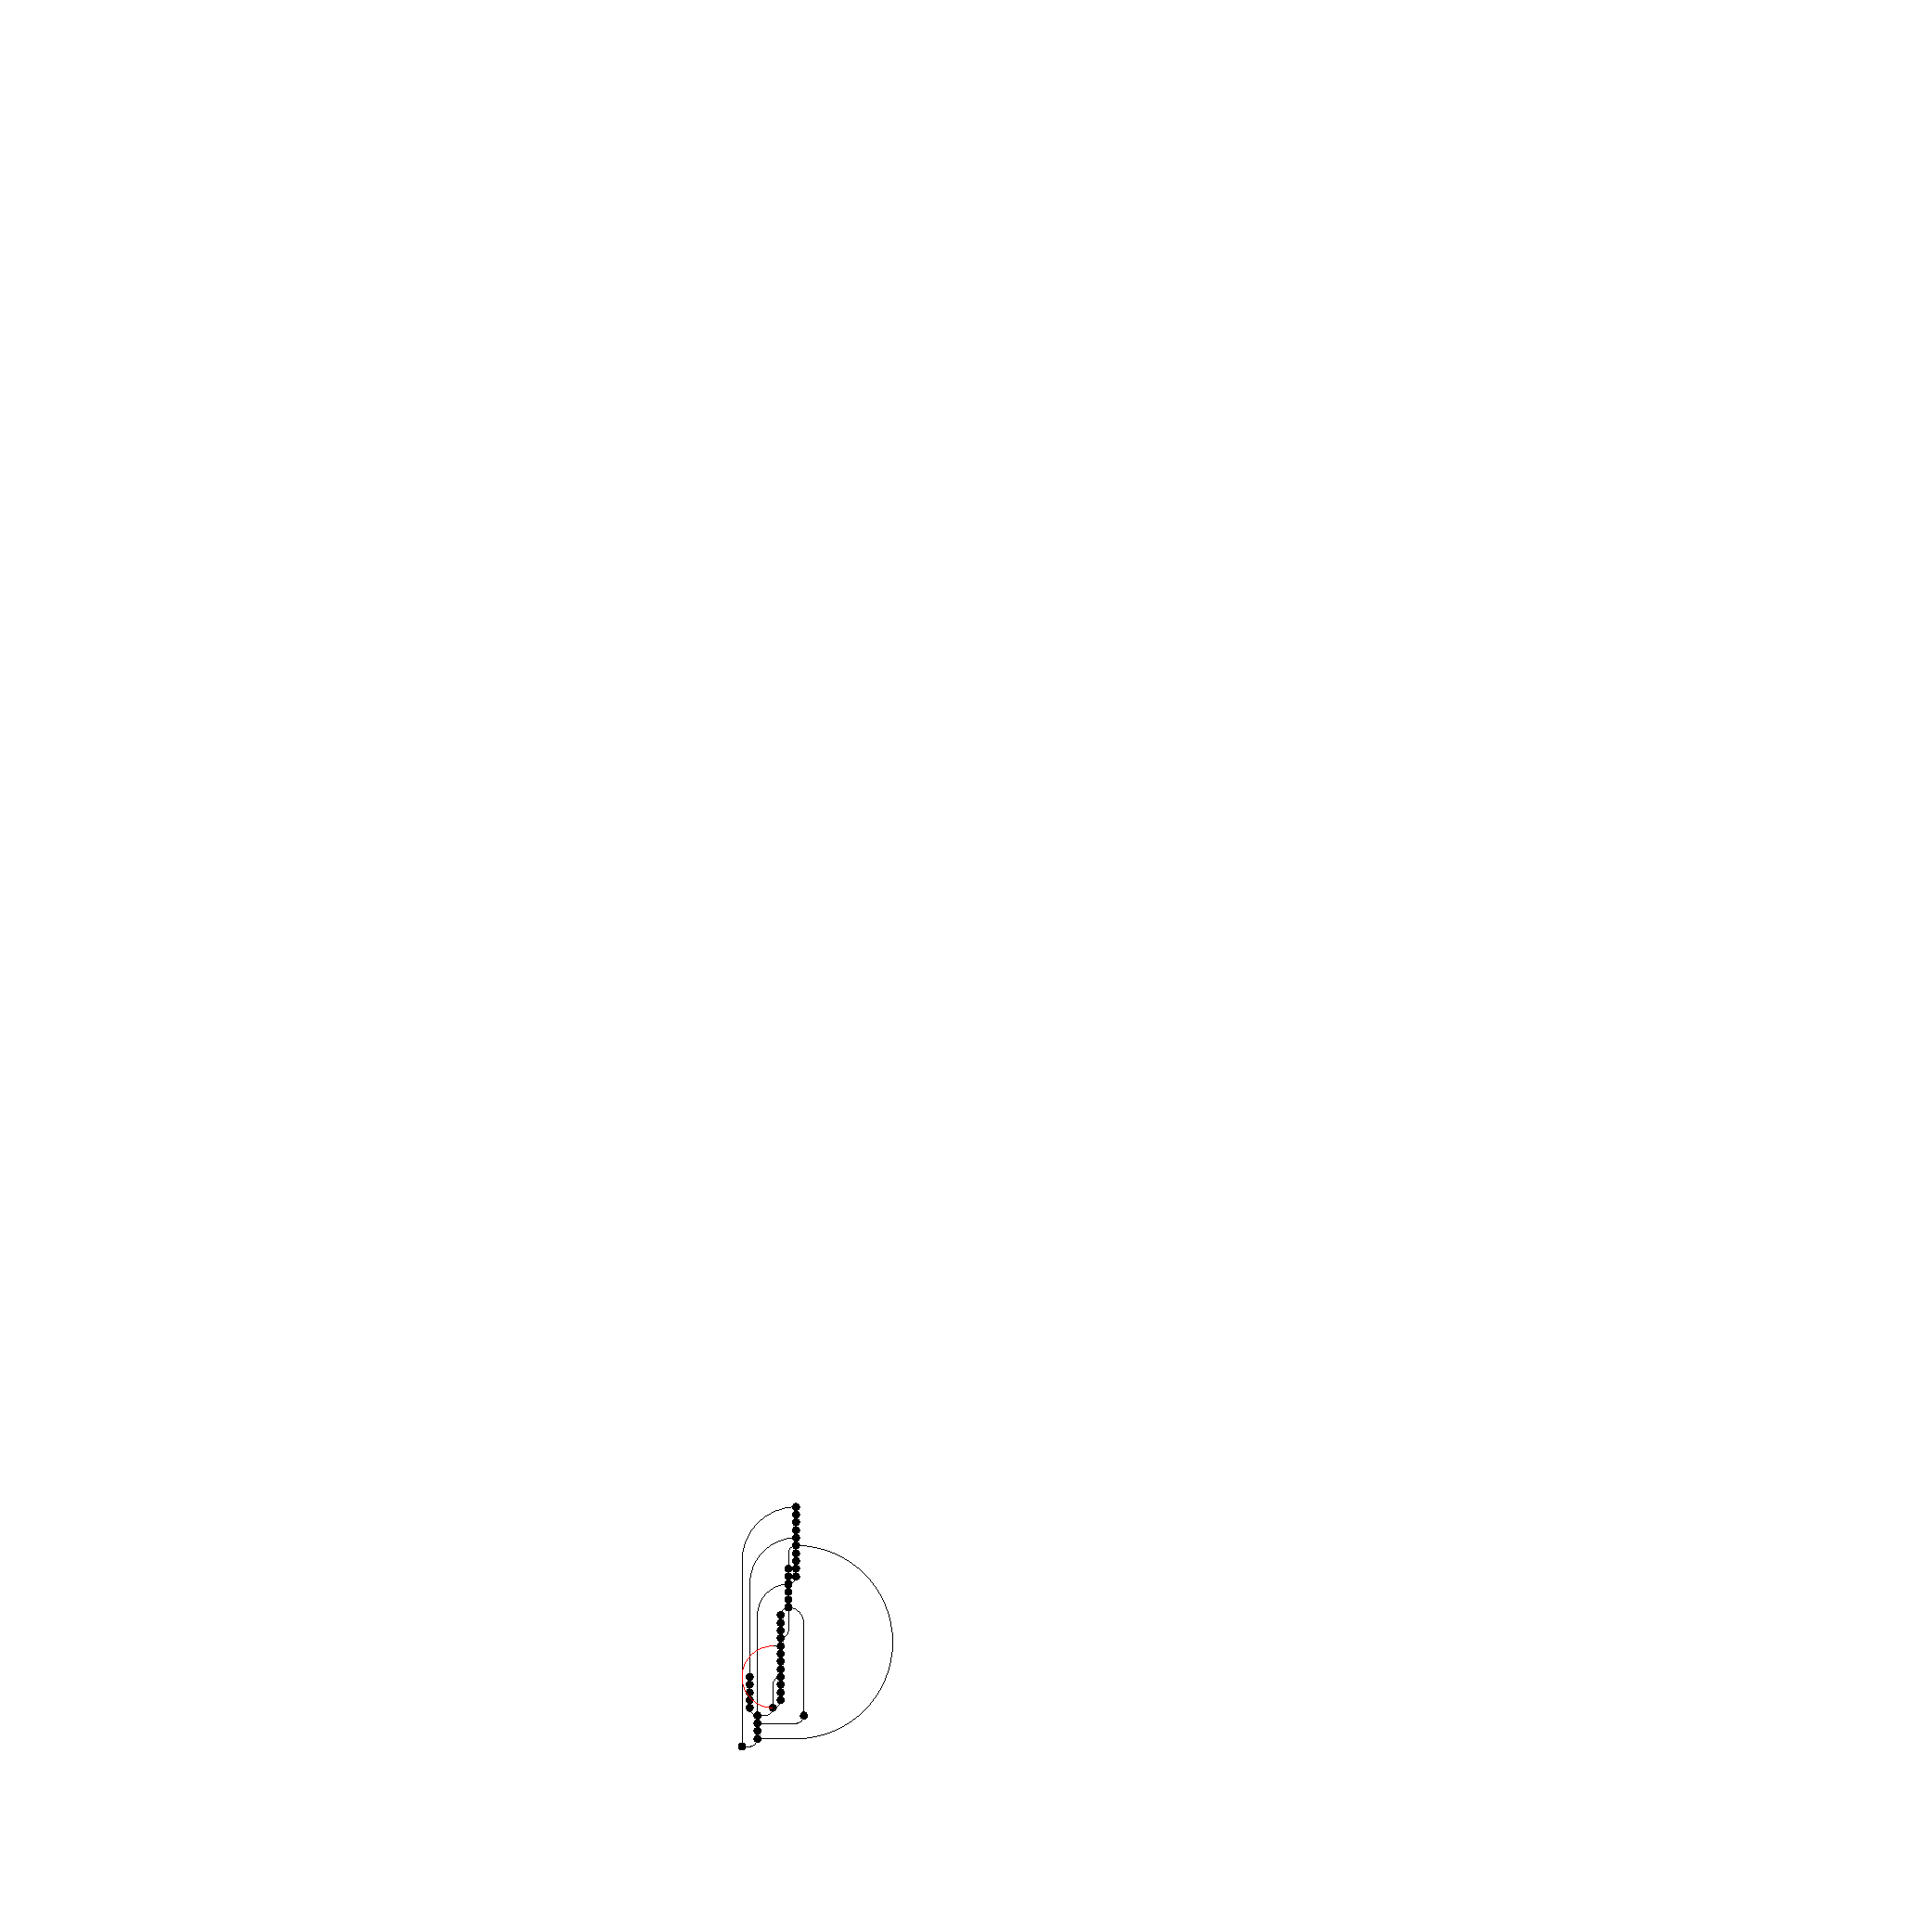
\includegraphics[scale=.8]{hugeGraph/isntPlanar}}
        \quad
        \subcaptionbox{Einige Korrekturen, die Zeichnung ist bereits überschneidungsfrei und benötigt $23 \times 31 = 713$ Gitterpunkte.\label{fig:smoothBadnessCorrected}}[0.4\textwidth]
            {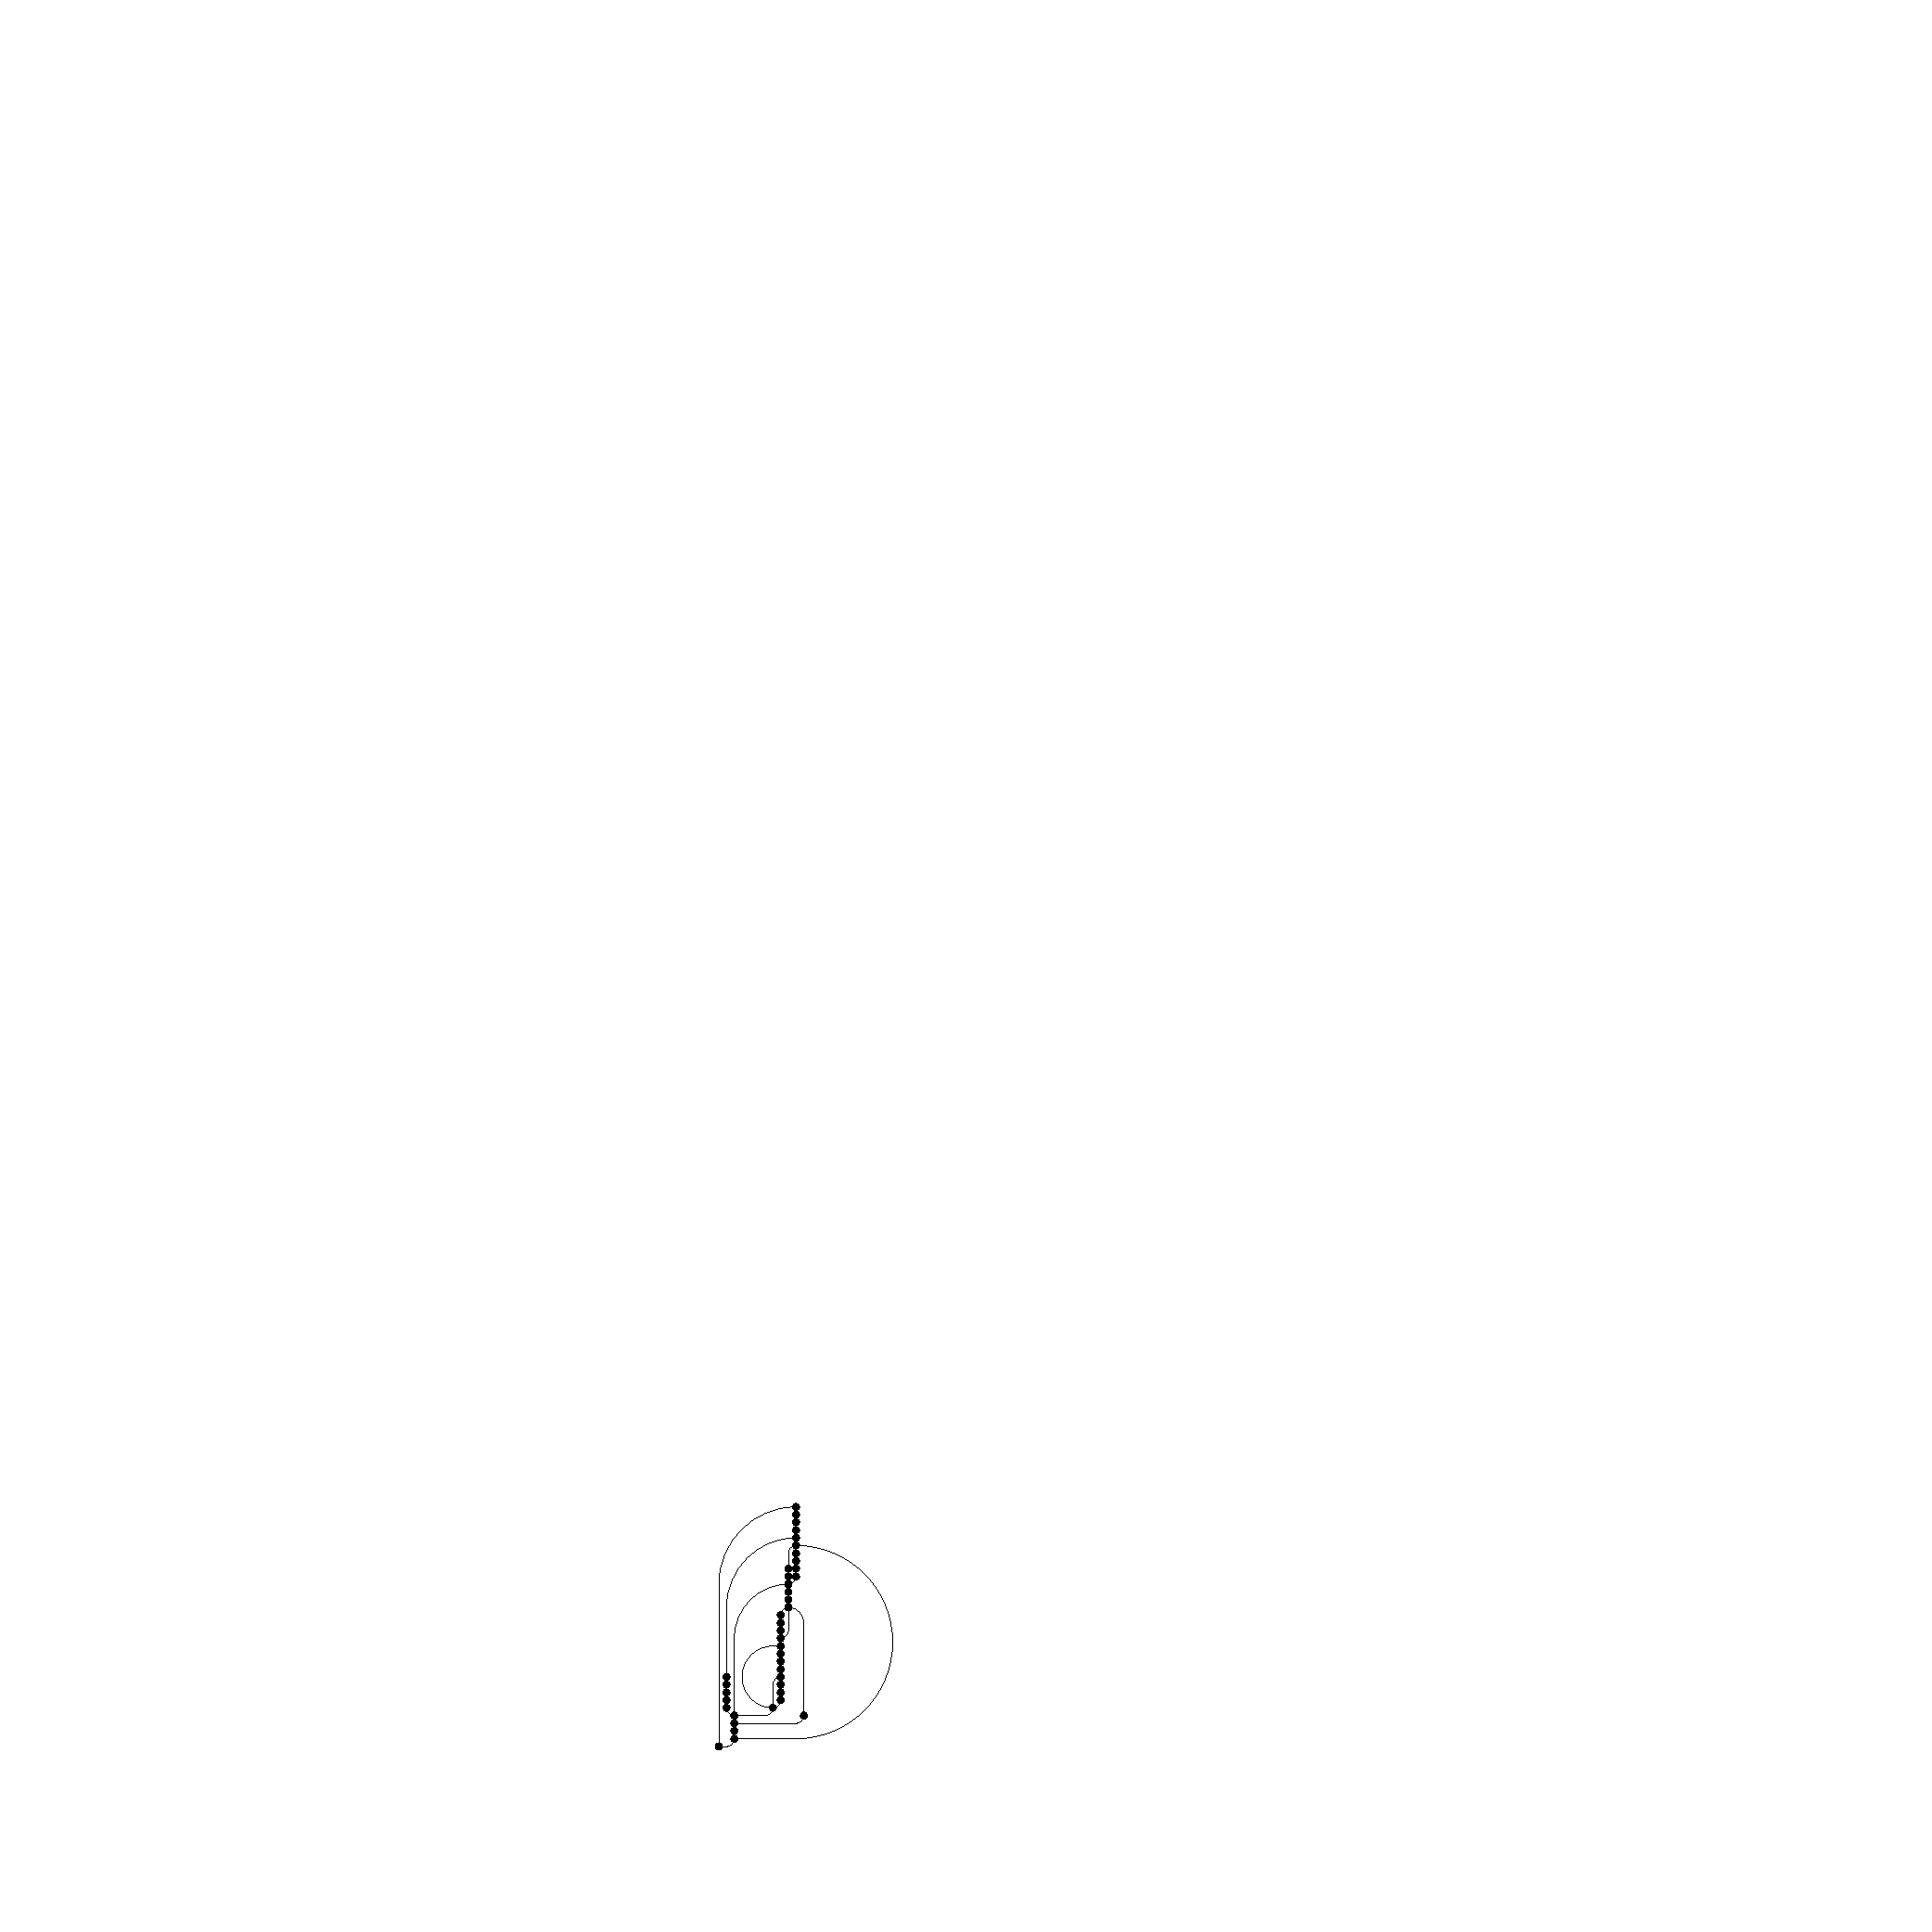
\includegraphics[scale=.8]{hugeGraph/isSmaller}}
        \quad
        \subcaptionbox{Durch die Korrektur der Steigung der L"~Kante im unteren, rechten Bereich muss der Knoten an der C"~Kante rechts weit nach oben verschoben werden, was wiederum die beiden L"~Kanten links durch die Korrektur der Steigung stark vergrößert. Der Graph benötigt $120 \times 82 = 9840$ Gitterpunkte. \label{fig:smoothBadnessShowing}}
            {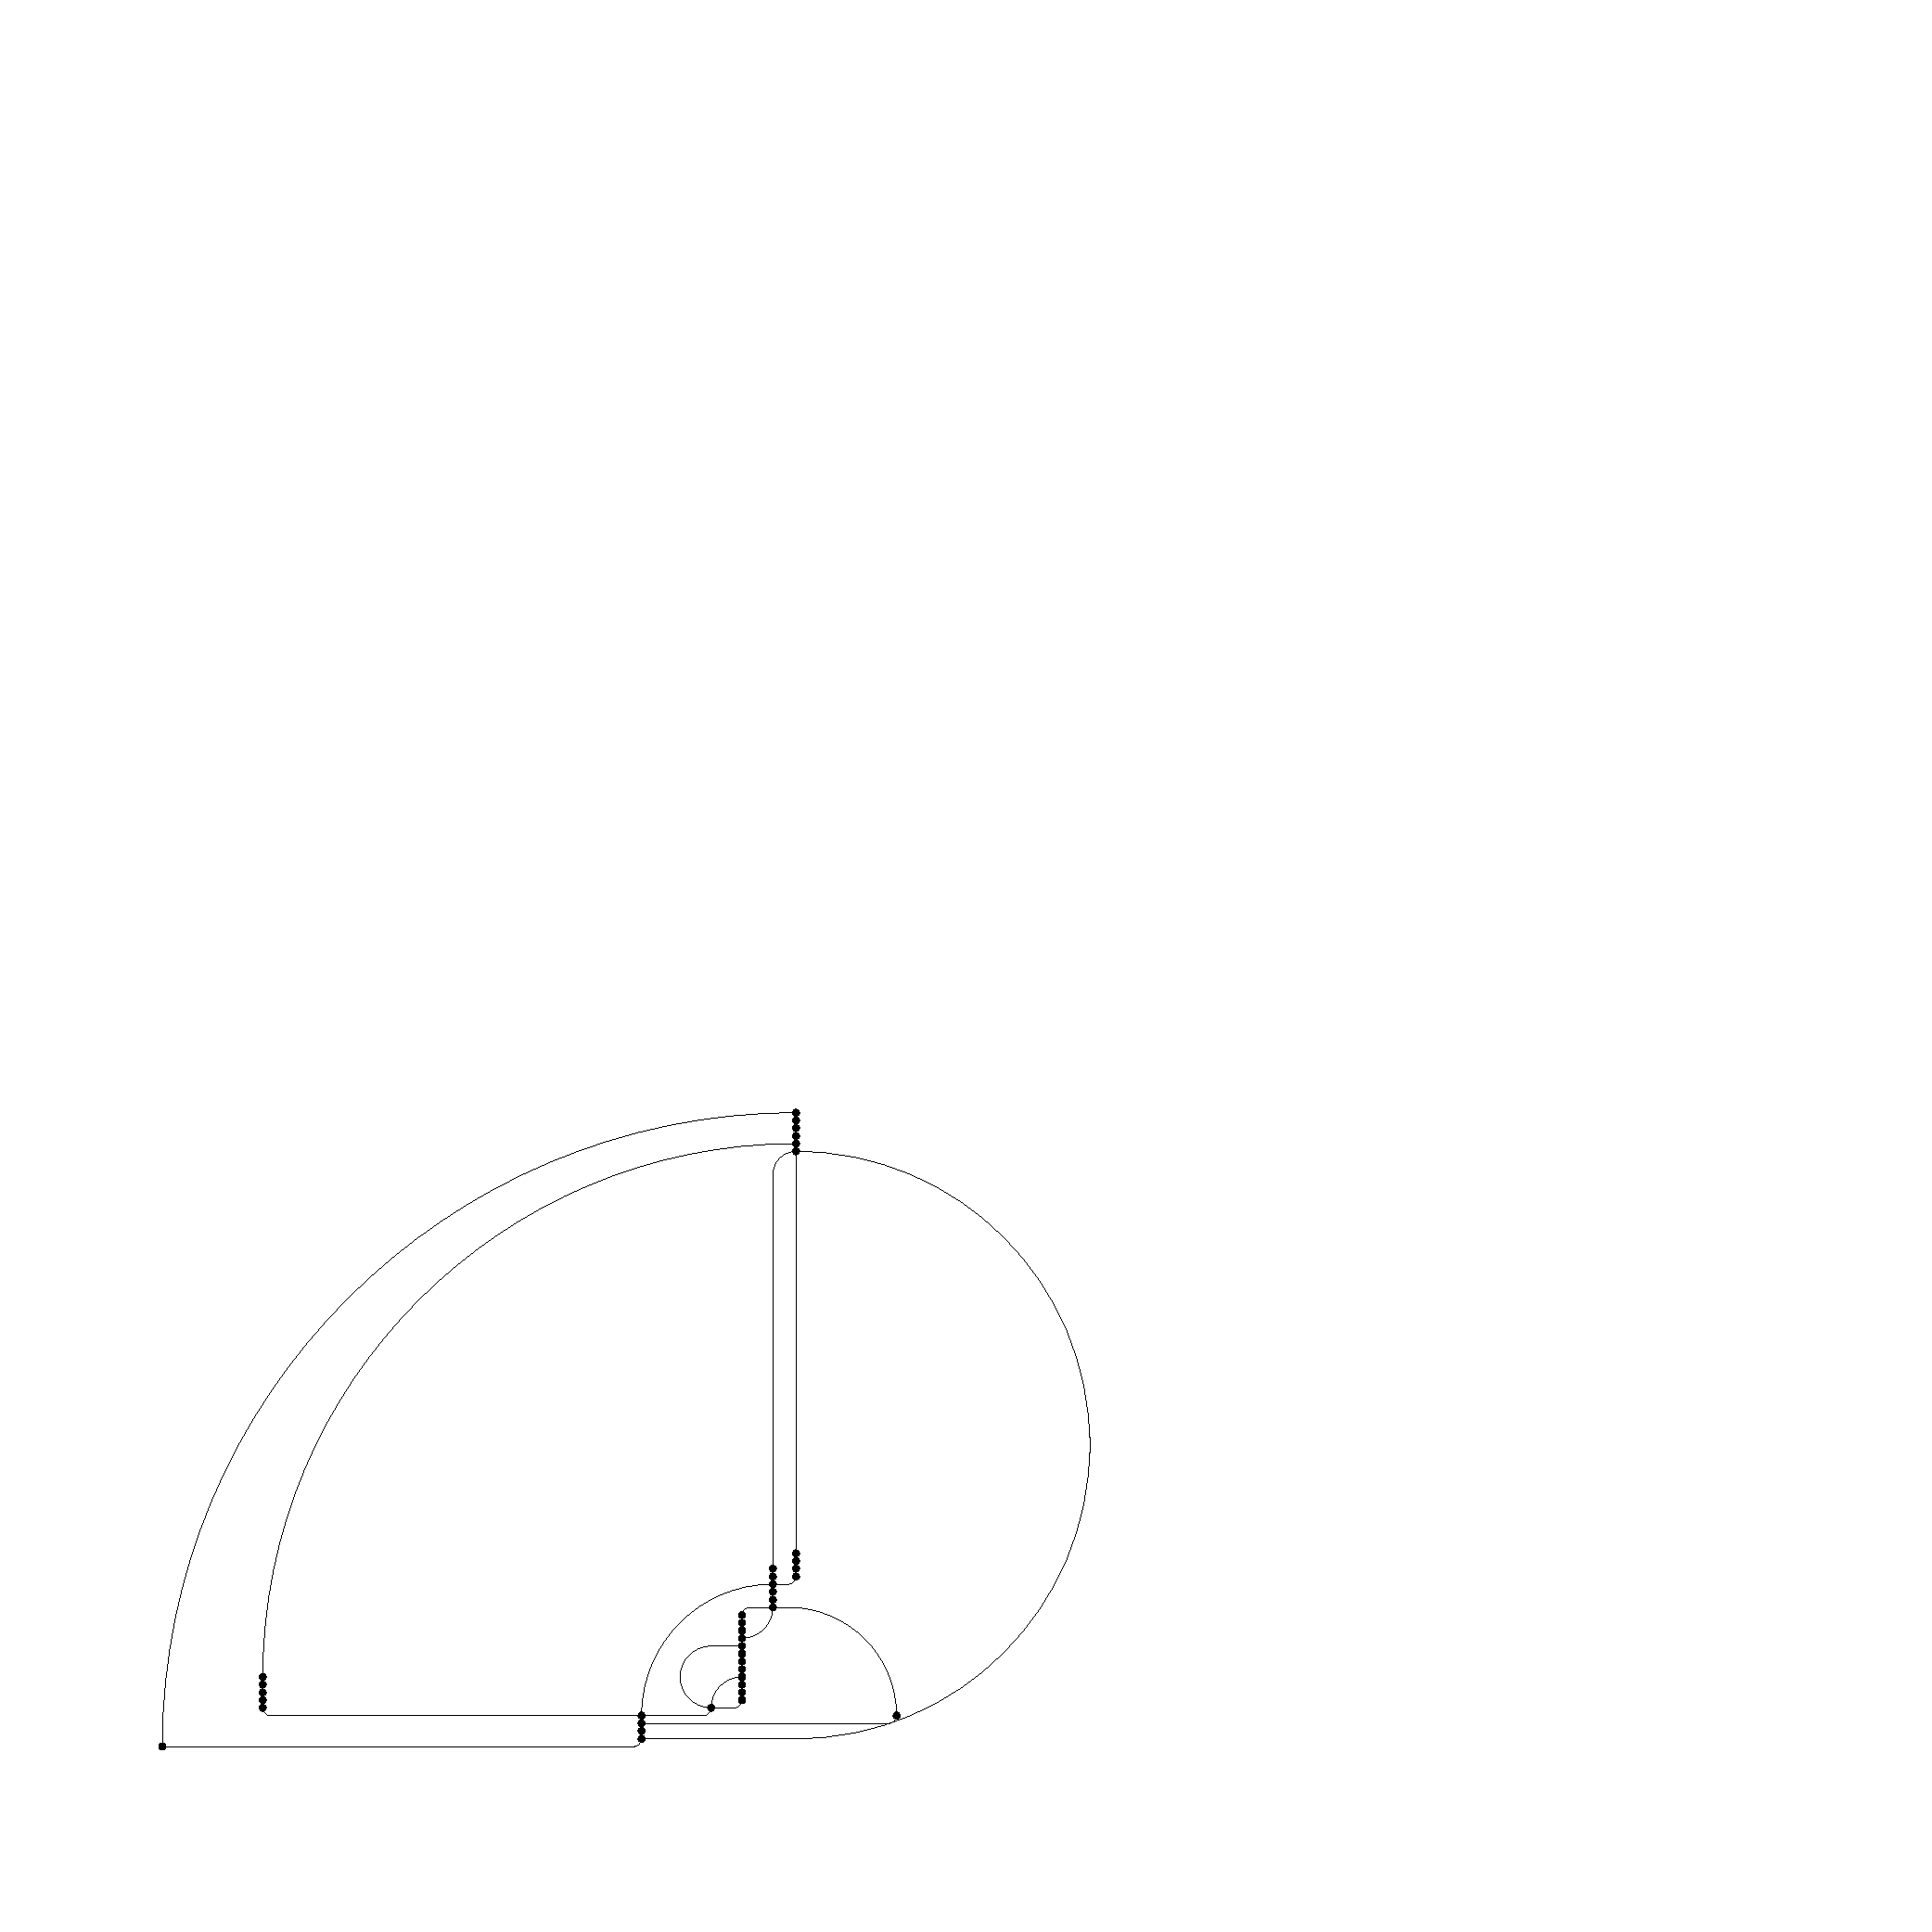
\includegraphics[scale=.8]{hugeGraph/isHuge}}
 
 
        \caption{Ein Graph mit 40 Knoten, der sich stark vergrößert, wenn die Korrektur der Steigungen angewandt wird. Die drei Zeichnungen sind hier mit derselben Gittergröße abgebildet und geben somit die Größenverhältnisse korrekt wieder.}
        \label{fig:smoothBadness}
\end{figure}

% this is grafo7046
\begin{figure}[h]
        \centering
       \subcaptionbox{Das orthogonale Layout ohne Komprimierung ist 47 Gittereinheiten hoch.\label{fig:smoothOknessRaw} }[0.3\textwidth]
            {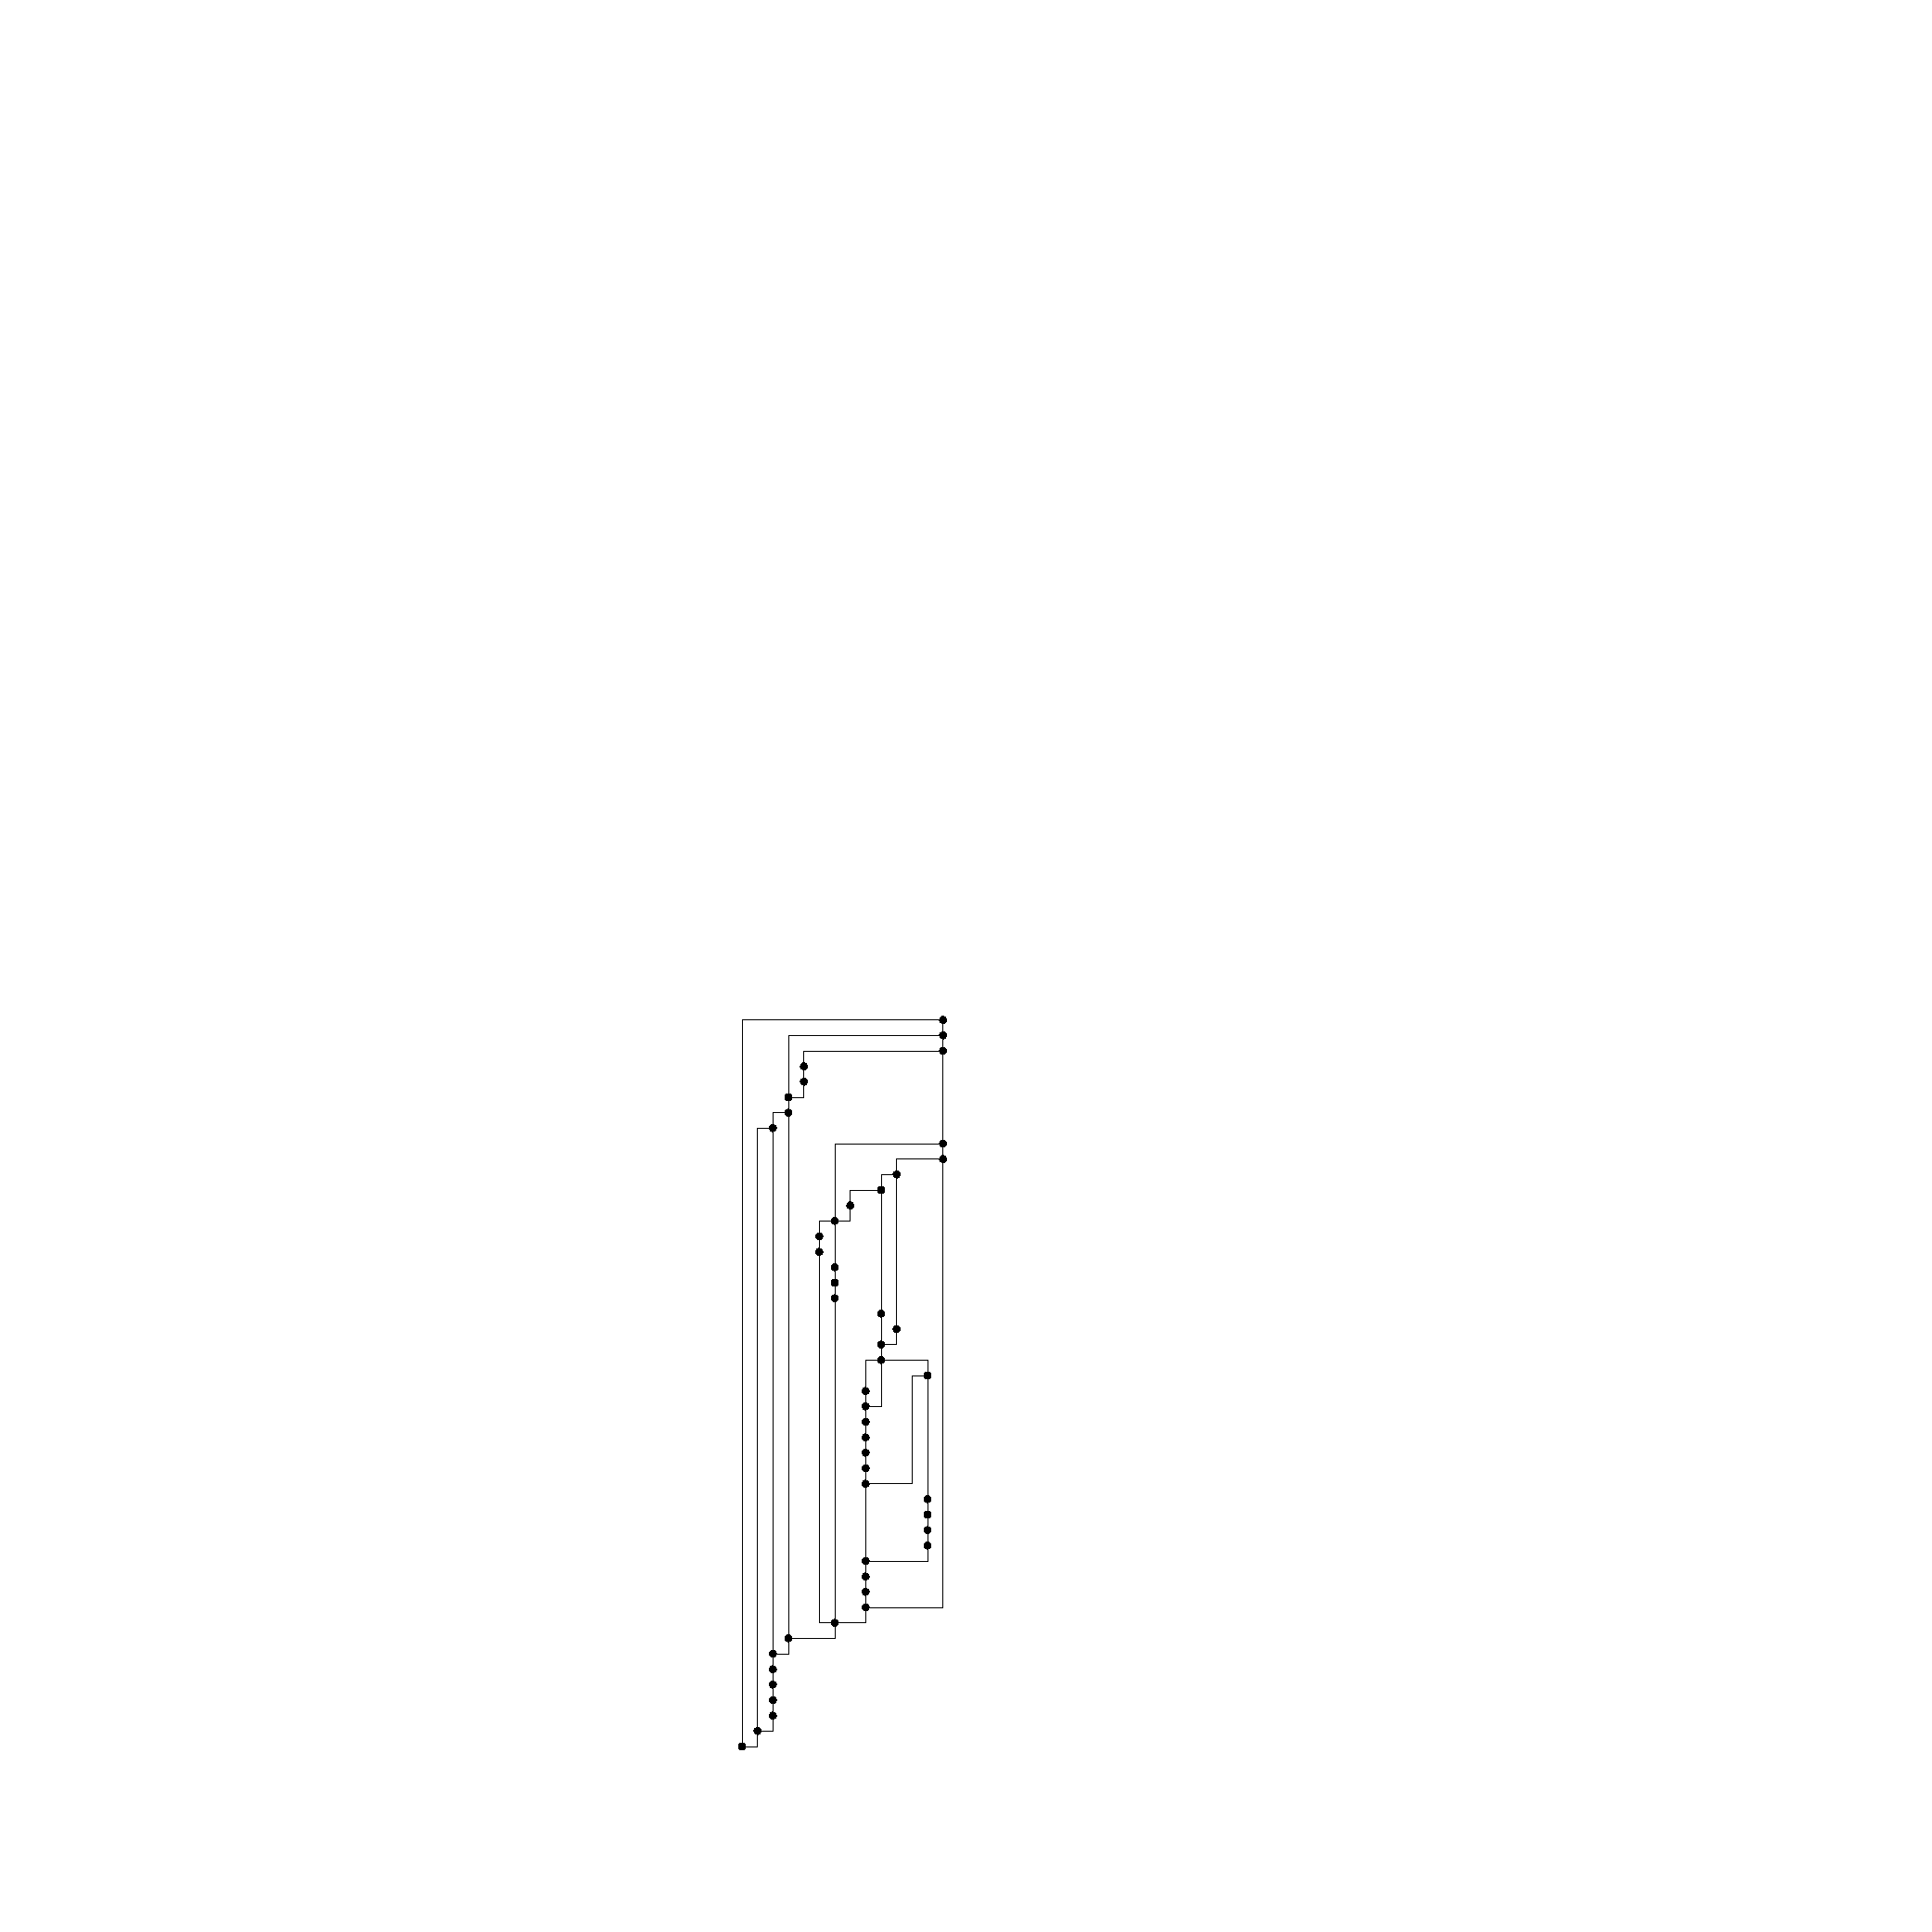
\includegraphics[scale=.7]{compliantGraph/isOrthogonalButUncompressed}}
        \quad
       \subcaptionbox{Nach Komprimierung bleiben 33 Gittereinheiten Höhe.\label{fig:smoothOknessCompressed} }[0.3\textwidth]
            {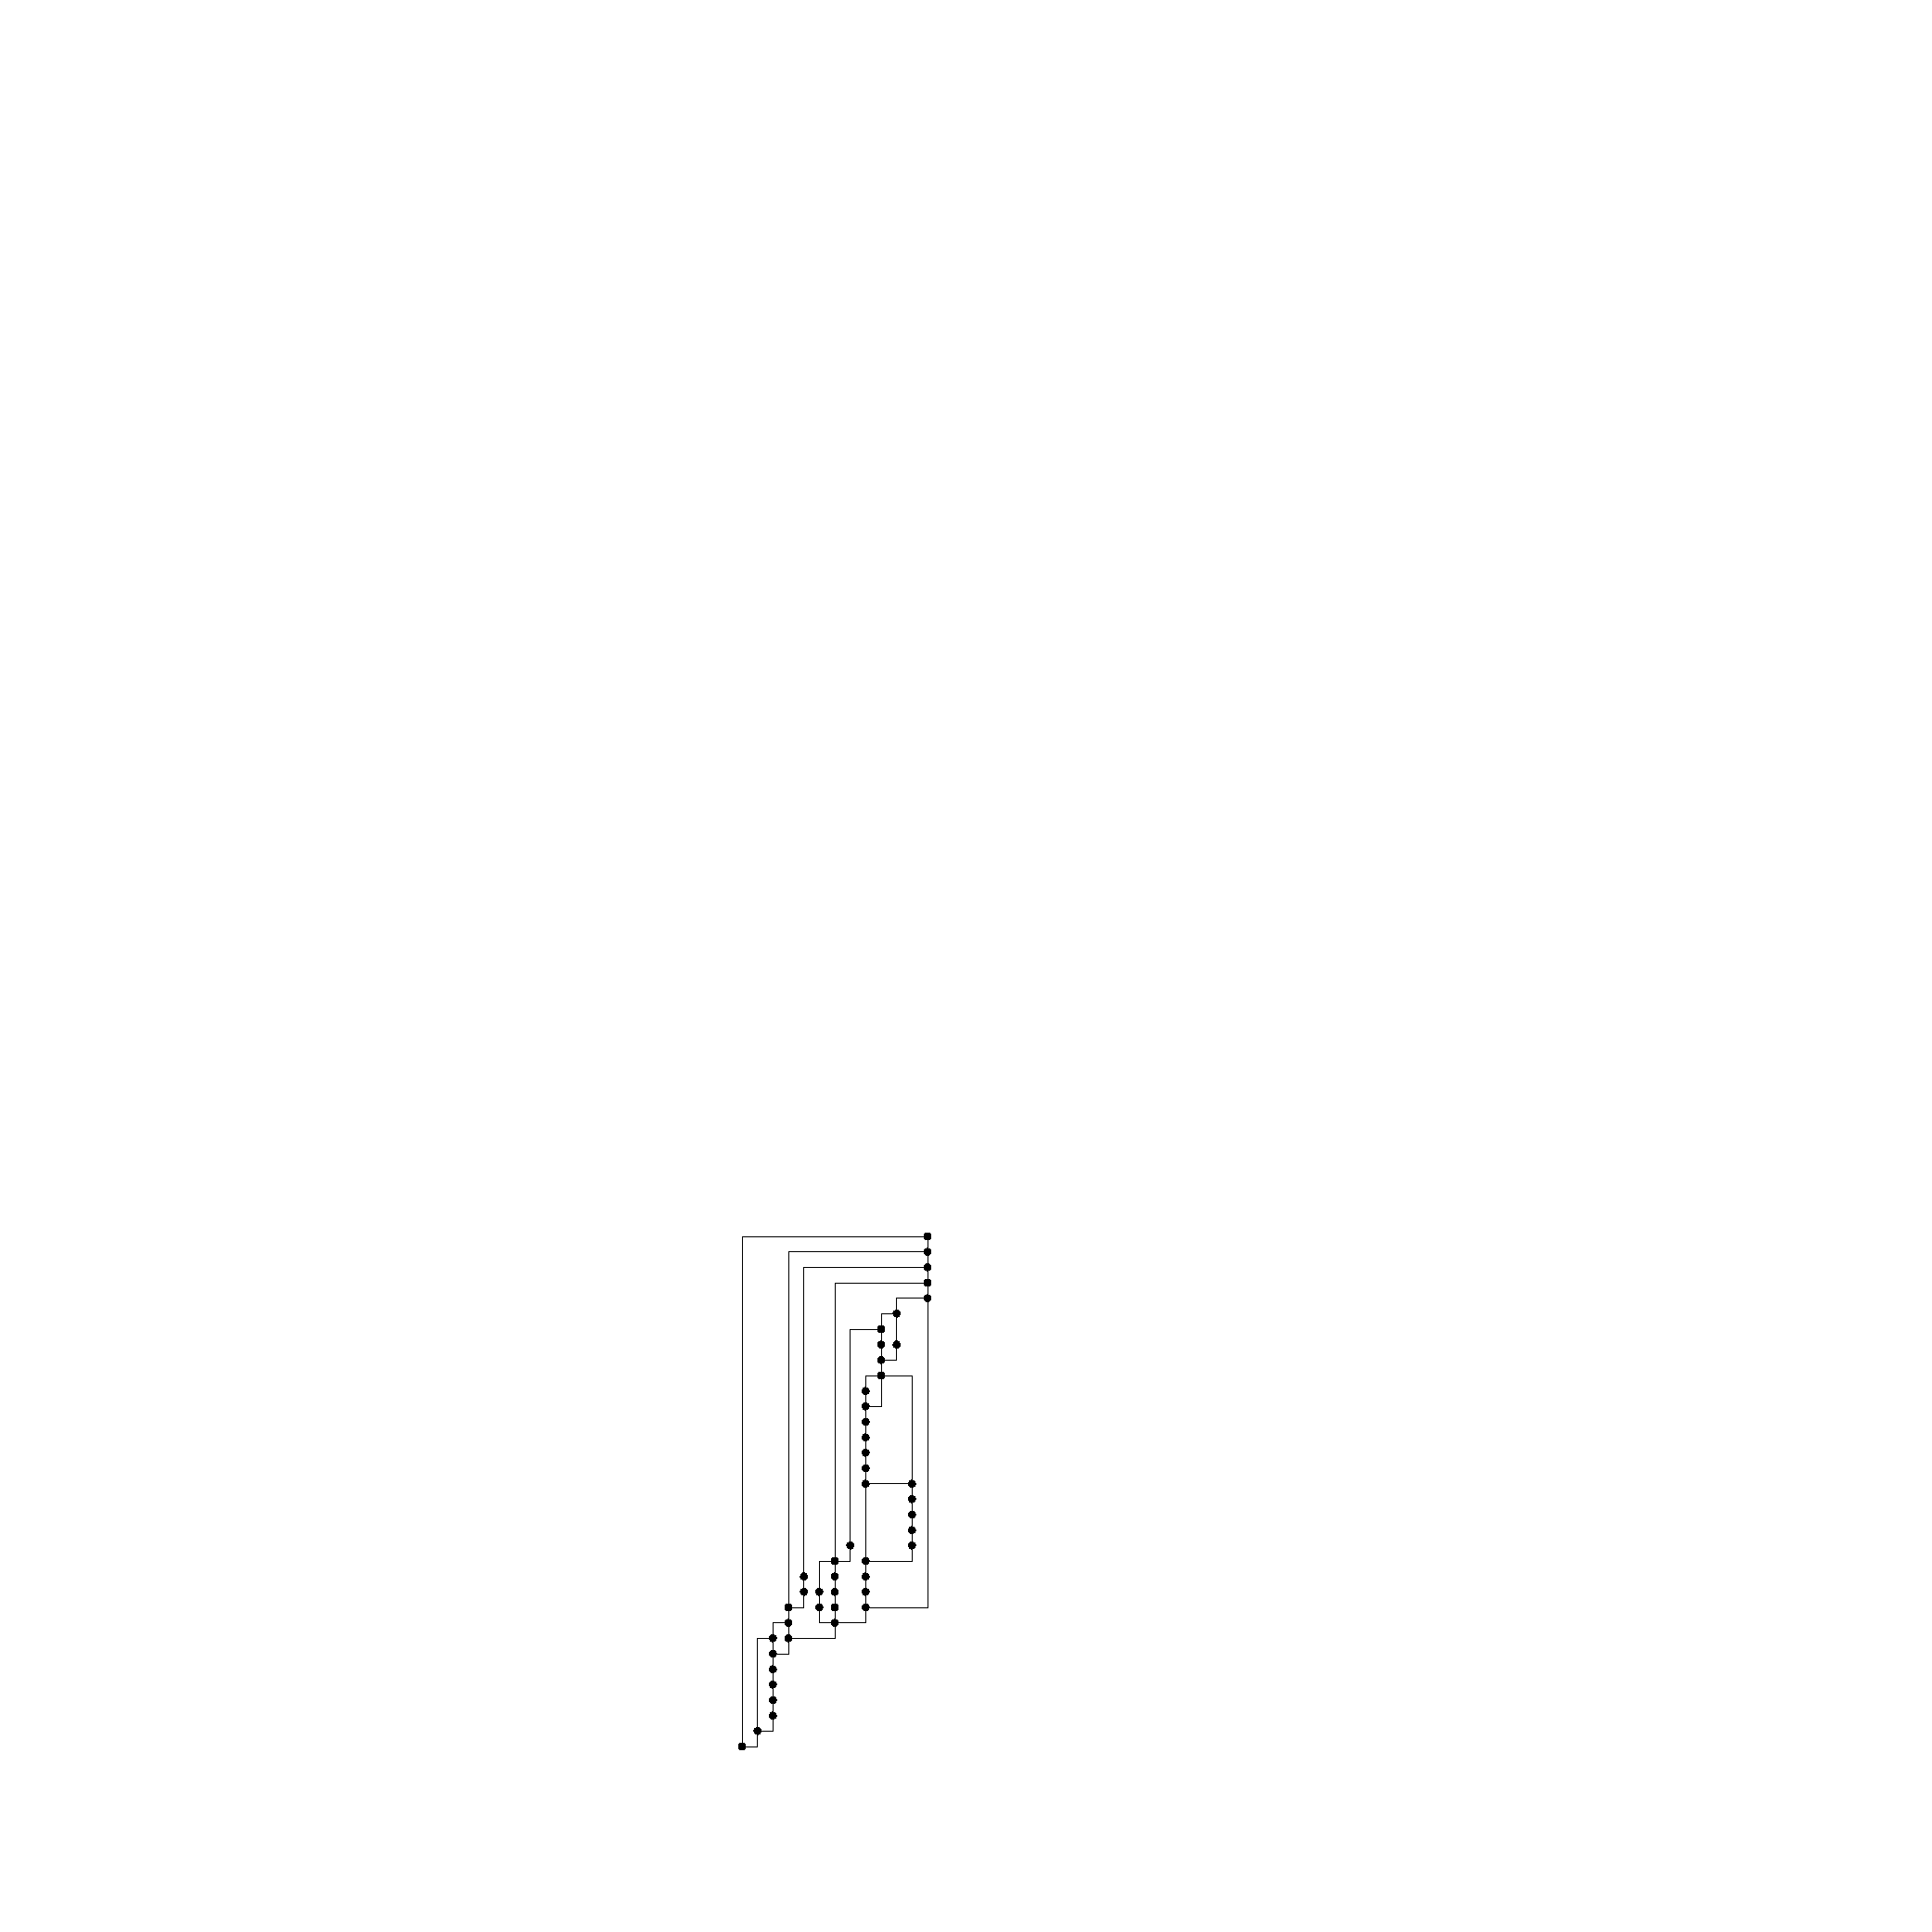
\includegraphics[scale=.7]{compliantGraph/isOrthogonal}}
        \quad
       \subcaptionbox{Auch die glatt"=orthogonale Zeichnung ist nur 12 Gittereinheiten breit.\label{fig:smoothOknessSmooth} }[0.3\textwidth]
            {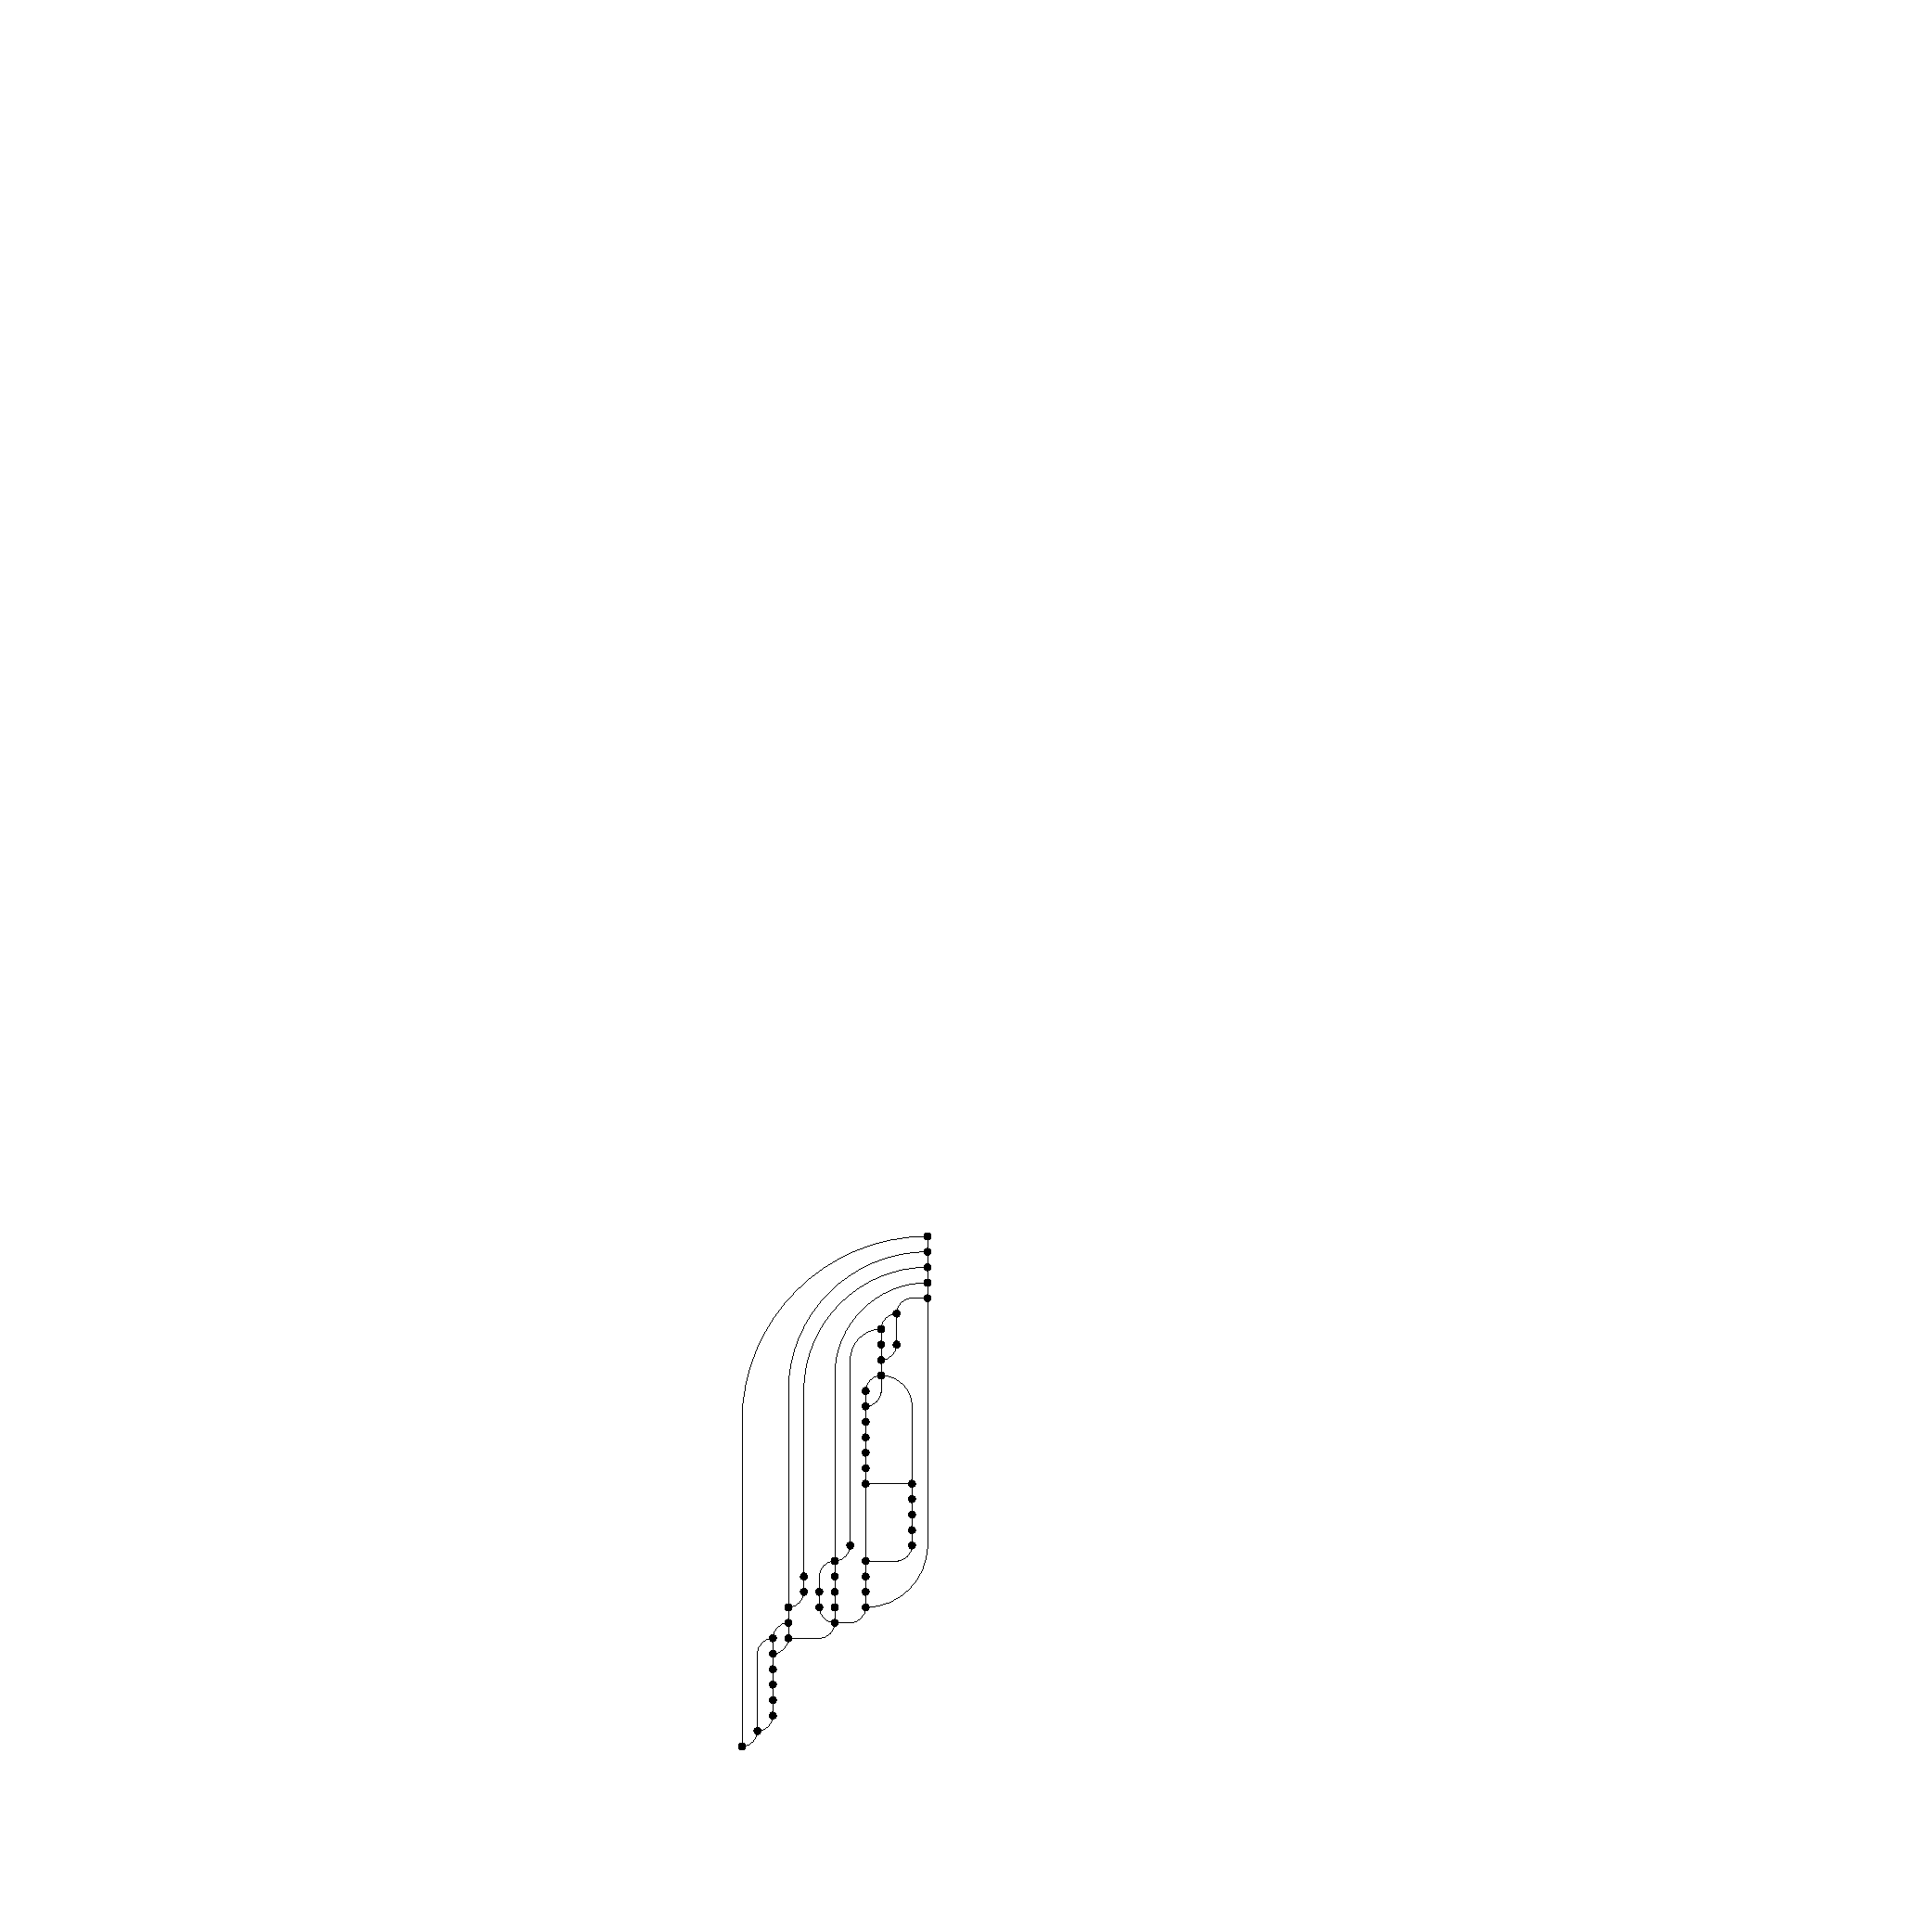
\includegraphics[scale=.7]{compliantGraph/isOk}}
        \quad
       \subcaptionbox{Durch die Korrektur der Steigungen der L"~Kanten wächst die Breite auf 45 Gittereinheiten.\label{fig:smoothOknessHugeAgain} }
            {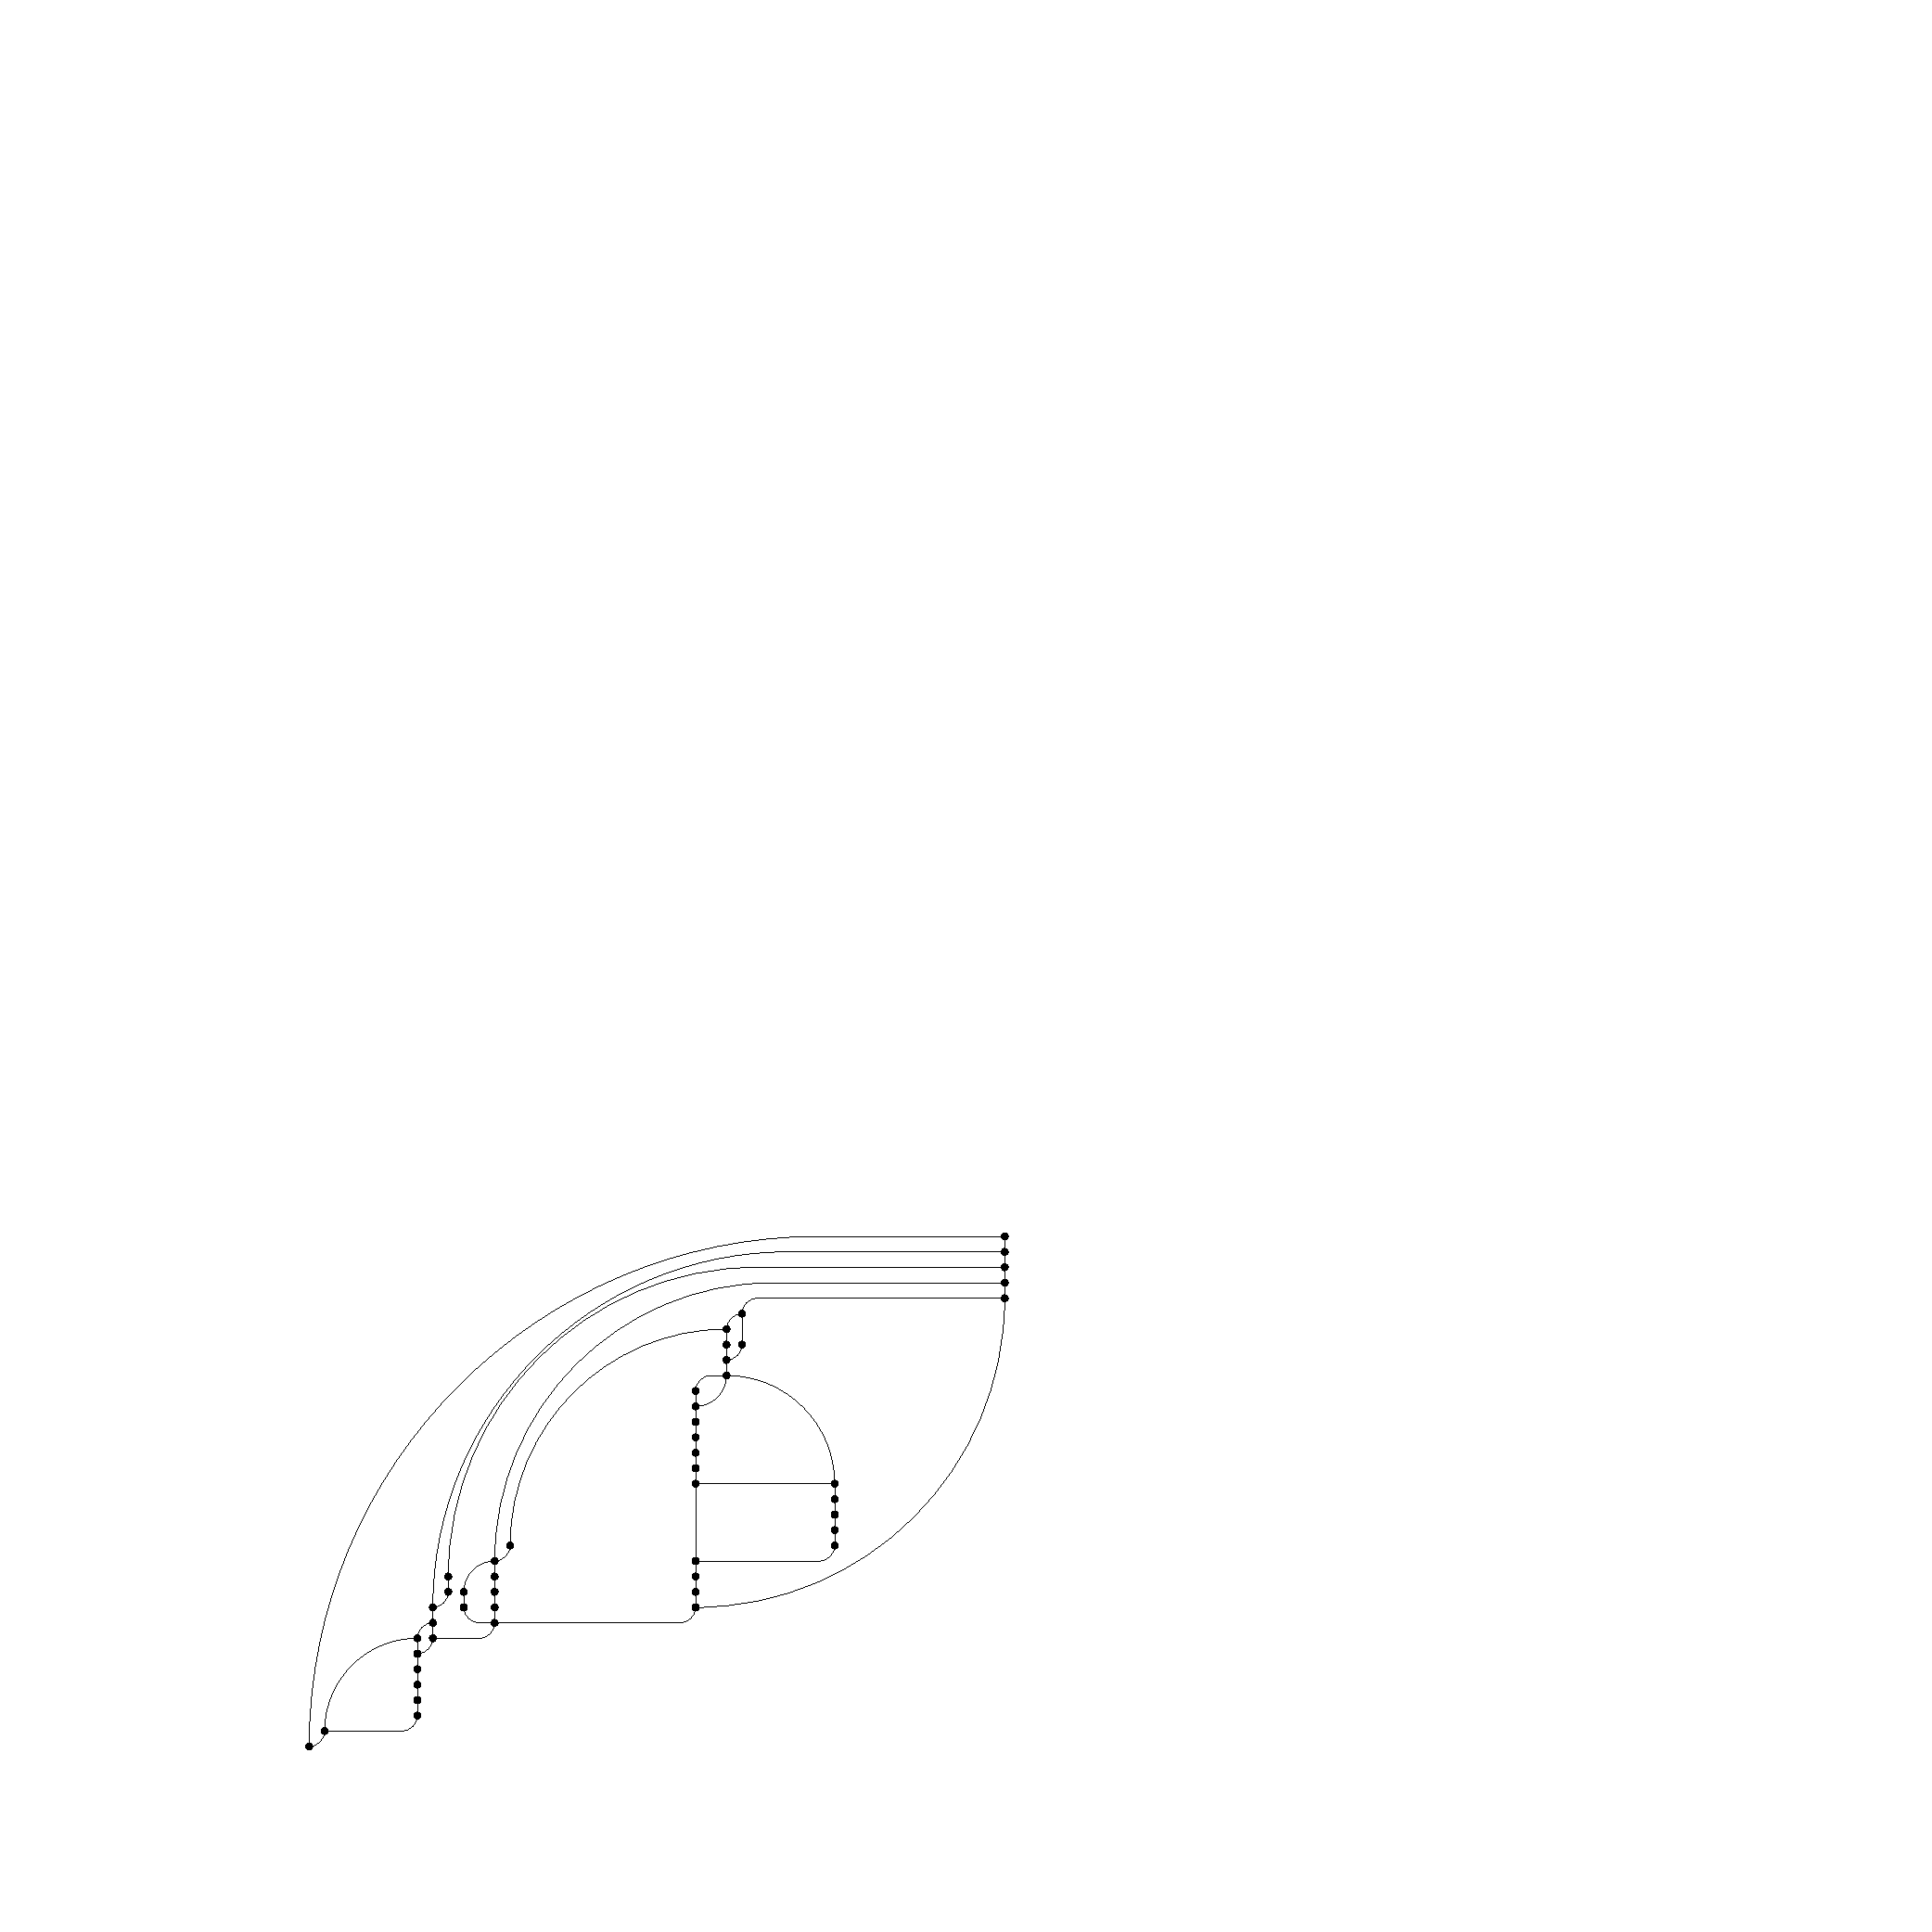
\includegraphics[scale=.7]{compliantGraph/isHuge}}
 
 
        \caption{Ein Graph mit 48 Knoten, dessen orthogonales Layout auch ein planares glatt"=orthogonales Layout darstellt. Die glatt"=orthogonale Zeichnung enthält nur I"~~und L"~Kanten. Die drei Zeichnungen sind hier mit derselben Gittergröße abgebildet und geben somit die Größenverhältnisse korrekt wieder.}
        \label{fig:smoothOkness}
\end{figure}



\chapter{Schlussfolgerungen und Ausblick}
\label{chap:outro}

Abschließend lässt sich sagen, dass der Algorithmus bis auf einen Grenzfall mit C"~Kanten detailliert für die Implementierung aufgearbeitet werden konnte. In Abschnitt~\ref{sec:sc2makePlanarAlgo} wurden zahlreiche Unterschiede und Ergänzungen zur Beschreibung von Alam et al.~\cite{smooth-13} aufgezählt, deren Notwendigkeit sich während der Implementierung aufgezeigt hat.

Es wurden Verbesserungen vorgenommen, indem mehrere Plateaus auf einer Höhe gezeichnet wurden und die Korrektur der Steigung ausgesetzt wird, wenn sie nicht nötig ist. Diese Verbesserungen sorgen in einigen Fällen für eine enorme Reduzierung des Flächenbedarfs der Zeichnungen und stellten sich für manche Graphen als nötig heraus, um sinnvoll nutzbare Zeichnungsgrößen zu erhalten.

Das Finden von Schnitten durch den Graphen wurde so systematisiert, dass in jedem Schritt nur die beiden Ports einer Kante betrachtet werden müssen, um einen Schnitt durch den Graphen zu erstellen. Die Schnitte wurden von Alam et al.~\cite{smooth-13} als Hauptwerkzeug zum Anpassen des Graphen erdacht, wurden jedoch an der geometrischen Repräsentation der Kanten definiert. Für die Implementierung ist es hilfreich, wenn die Berechnungsvorschrift allein auf dem Graphen und der Portzuweisung basiert, sodass beim Finden des Schnitts keine aufwändigen geometrischen Berechnungen durchgeführt werden müssen.

Die Kanten können mit der Information der Lage der beiden Endpunkte und den beiden Ports schon in Liniensegmente und Kreisbögen umgerechnet werden. Dies erleichtert Implementierungen erheblich, da beim Bearbeiten der Zeichnung nicht die Kanten oder ihre Darstellung in der Zeichnung transformiert werden müssen, sonder nur die Knotenpositionen. Werden weitere Informationen zum Aussehen einer Kante benötigt, können sie mit den Knotenpositionen und der Portzuweisung berechnet werden.

Das Prüfen auf Überschneidungen von Kanten wurde geometrisch gelöst. Auf Grundlage der dargestellten Funktionsweise ließe sich der Algorithmus implementieren, um beispielsweise weitere Verbesserungen empirisch zu prüfen, oder es könnten für Teilaspekte noch effizientere Algorithmen eingesetzt werden.

Die Ergebnisse der empirischen Untersuchung zeigen, dass der Algorithmus mit den hier entwickelten Anpassungen schon gute Ergebnisse liefern kann, es aber auch noch Spielraum für Verbesserungen gibt. Die Laufzeit des Algorithmus lag in einem akzeptablen Rahmen und der Flächenbedarf der Zeichnungen 

Dank der Implementierung konnte der Algorithmus auf eine Vielzahl unterschiedlicher Graphen angewendet werden. Hierbei ergeben sich Einblicke in die Arbeitsweise des Algorithmus: Durch die Visualisierung der Anwendung auf größere Graphen erlangt man eine Intuition für die Funktionsweise des Algorithmus.

Weiterführende Untersuchungen könnten eine Anpassung der $st$-Ordnung und der Einbettung für die Optimierung der Zeichnungen untersuchen. Biedl~\& Kant ~\cite{biedl+kant-98} entwickelten bereits eine Reihe von Optimierungen für orthogonale Zeichnungen, von denen geprüft werden könnte, ob sie sich auf glatt"=orthogonale Zeichnungen übertragen lassen. Sie schlagen beispielsweise vor, einen Knoten mit möglichst kleinem Grad als Ausgangsknoten $s$ für die $st$-Ordnung zu wählen. Die Untersuchung der Auswirkungen einer solchen Optimierung auf die glatt"=orthogonalen Zeichnungen könnte die Grundlage für weitere Forschungen bilden.

Des weiteren wäre es wünschenswert, die Implementierung und die damit verbundenen Auswertungen von den Beschränkungen auf planare und zweifach zusammenhängende Graphen zu lösen, denn diese Beschränkungen stehen einer praktischen Anwendung noch im Weg: Aus Anwendersicht sind diese Beschränkungen nicht sehr nachvollziehbar und der Wunsch liegt nahe, allgemeinere Graphen auch visualisieren zu können.

\begin{figure}[h]
  \centering
  \includegraphics{exampleA/smoothHanddrawn}
  \caption{Manuell erstellte glatt"=orthogonale Zeichnung von Beispielgraph $G_\text{E}$.}
  \label{fig:exampleAsmoothHanddrawn}
\end{figure}

Insgesamt gibt es noch viel Verbesserungspotential für den Algorithmus. Als abschließendes Beispiel sei in Abbildung~\ref{fig:exampleAsmoothHanddrawn} eine handgezeichnete glatt"=orthogonale Darstellung des Graphen $G_\text{E}$ aus Kapitel~\ref{chap:basics} gegeben. Diese Visualisierung überbietet die maschinell erstellten Zeichnungen aus Abbildung~\ref{fig:exampleAsmooth} im Vergleich: Sie hat Komplexität~1 statt~2 und~3 bei gleichzeitig geringerem Platzbedarf: $3 \times 3 = 9$ statt $3 \times 4 = 12$ und $7 \times 6 = 42$.


\bibliographystyle{mybabalpha-fl}
\bibliography{mybib}

%\listoffigures

\newpage

Hiermit versichere ich, dass ich die vorliegende Arbeit selbständig verfasst und keine
anderen Hilfsmittel und Quellen als die angegebenen benutzt habe. Weiterhin versichere
ich, die Arbeit weder bisher noch gleichzeitig einer anderen Prüfungsbehörde vorgelegt
zu haben.
\\ \\ \\ \\
Würzburg, den \makebox[3cm]{\hrulefill},  \hspace{.5cm} \makebox[7cm]{\hrulefill}\\
\makebox[11.75cm][r]{(Bernhard Häussner)}


\end{document}
